
\documentclass[12pt]{article}
\usepackage[utf8]{inputenc}
\renewcommand{\baselinestretch}{1.5}

\newcommand*{\SuperScriptSameStyle}[1]{%
  \ensuremath{%
    \mathchoice
      {{}^{\displaystyle #1}}%
      {{}^{\textstyle #1}}%
      {{}^{\scriptstyle #1}}%
      {{}^{\scriptscriptstyle #1}}%
  }%
}

\newcommand{\oneS}{\ensuremath{{}^{\textstyle *}}}
\newcommand{\twoS}{\ensuremath{{}^{\textstyle **}}}
\newcommand{\threeS}{\ensuremath{{}^{\textstyle **}\oneS}}

\usepackage{amsmath}
\usepackage{amsfonts}
\usepackage{eurosym}
\usepackage[hmargin=2.5cm,vmargin=3.5cm]{geometry}
\usepackage{graphicx}
\graphicspath{
  {images/}
  {figures/}
  {figures/layout/}
  {figures/analysis/}
  {../code/outputs/south_america/results/model1_lgbm/}
  {../code/outputs/south_america/results/model1_rf/}
  {../code/outputs/south_america/results/forward/lgbm/}
  {../code/outputs/south_america/results/forward/rf/}
  {../code/outputs/south_america/results/spatial_cv_visualisation/}
  {../code/outputs/usa/results/model2_lgbm/}
  {../code/outputs/usa/results/model2_rf/}
  {../code/outputs/usa/results/forward/lgbm/}
  {../code/outputs/usa/results/forward/rf/}
  {../code/outputs/usa/results/spatial_cv_visualisation/}
  {../code/outputs/se_asia/results/model3_lgbm/}
  {../code/outputs/se_asia/results/model3_rf/}
  {../code/outputs/se_asia/results/forward/lgbm/}
  {../code/outputs/se_asia/results/forward/rf/}
  {../code/outputs/se_asia/results/spatial_cv_visualisation/}
}
\usepackage[font+=small,labelfont=bf, skip=0pt]{caption,subcaption}
\usepackage{float}
\usepackage{newunicodechar}
\newunicodechar{₂}{$_2$}
\newunicodechar{≈}{\approx}
\usepackage{multirow}
\usepackage{color}
\usepackage{setspace}
\usepackage{footmisc}
\usepackage{natbib}
\usepackage{pdflscape}
\usepackage{array}
\usepackage[debugshow]{tabulary}
\usepackage[debugshow]{tabularx}
\usepackage{amssymb}
\usepackage{ragged2e}
\usepackage[para,online,flushleft]{threeparttable}
\usepackage[etex=true,export]{adjustbox}
\usepackage{tablefootnote}
\usepackage[hidelinks]{hyperref}
\usepackage{ntheorem}
\usepackage{tikz}
\usepackage{lscape}
\usepackage{comment}
\usepackage{mathtools}
\usepackage{dsfont}
\usepackage{varwidth}
\usepackage{soul}
\usetikzlibrary{positioning,trees,fit,calc}

\newenvironment{changemargin}[2]{%
  \begin{list}{}{%
    \setlength{\topsep}{0pt}%
    \setlength{\leftmargin}{#1}%
    \setlength{\rightmargin}{#2}%
    \setlength{\listparindent}{\parindent}%
    \setlength{\itemindent}{\parindent}%
    \setlength{\parsep}{\parskip}%
  }%
  \item[]}{\end{list}}

\tikzstyle{level 1}=[level distance=3.5cm, sibling distance=4.0cm]
\tikzstyle{level 2}=[level distance=3.5cm, sibling distance=2cm]
\tikzstyle{bag} = [align=center]

\usepackage{booktabs}
\usepackage{longtable}
\geometry{left=2.54cm,right=2.54cm,top=2.54cm,bottom=2.54cm}
\usepackage{dcolumn}
\usepackage[toc,page]{appendix}
\renewcommand\appendixpagename{Appendix}
\usepackage[noabbrev,nameinlink,capitalise]{cleveref}

\providecommand{\keywords}[1]{\textbf{Keywords:} #1}
\crefname{appsec}{Section}{Appendices}

% --- Title page helpers ---
\usepackage{titling}
\onehalfspacing
\theoremstyle{break}
\newtheorem{definition}{Definition}
\newtheorem{assumption}{Assumption}
\newtheorem{theorem}{Theorem}
\newcolumntype{L}[1]{>{\raggedright\let\newline\\arraybackslash\hspace{0pt}}m{#1}}
\newcolumntype{C}[1]{>{\centering\let\newline\\arraybackslash\hspace{0pt}}m{#1}}
\newcolumntype{R}[1]{>{\raggedleft\let\newline\\arraybackslash\hspace{0pt}}m{#1}}

% --- Thesis metadata ---
\newcommand{\thesistype}{Master Thesis}
\newcommand{\studentname}{Gian-Luca Kaufmann}
\newcommand{\studentemail}{gikaufmann@ethz.ch}
\newcommand{\studentnumber}{20-913-166}
\newcommand{\thesistitle}{Predicting Protected Area Designations and Assessing Transition Risk under 30$\times$30}
\newcommand{\thesissubtitle}{}
\newcommand{\chair}{Chair of Energy and Climate Economics}
\newcommand{\department}{Department of Management, Technology, and Economics, ETH Zurich}
\newcommand{\supervisorblock}{%
  Prof.\ Dr.\ Lint Barrage, D-MTEC, ETH Zurich \\
  Dr.\ Patricio Velasquez, D-MTEC, ETH Zurich \\
  Dr.\ Chiara Colesanti Senni, Department of Finance, University of Zurich \\
  Elena\ Almeida, CETEx, London School of Economics and Political Science (LSE)}
\newcommand{\submissiondate}{April 2026}

% ===========================================================================
\begin{document}
% ===========================================================================

% ---------------------------------------------------------------------------
%  Title page
% ---------------------------------------------------------------------------
\begin{titlepage}
\thispagestyle{empty}

\vspace*{-1.5cm}
\noindent
\begin{minipage}[t]{0.49\textwidth}
  
\includegraphics[height=1.5cm]{figures/layout/eth_logo_black.pdf}
\end{minipage}
\begin{minipage}[t]{0.49\textwidth}
  \raggedleft
  
\includegraphics[height=1cm]{figures/layout/LOGO_MTEC.png}
\end{minipage}

\vspace*{2cm}
\begin{center}
{\LARGE\bfseries \thesistitle \par}
\vspace{0.4cm}
{\Large\bfseries \thesissubtitle \par}
\vspace{0.8cm}
{\large \thesistype \par}
\end{center}

\vspace*{2.0cm}
\begin{center}
{\large \studentname \par}
\vspace{0.25cm}
{\small \studentemail \par}
\vspace{0.25cm}
{\small \studentnumber \par}
\vspace{1.2cm}
{\small \submissiondate \par}
\end{center}

\vfill
\begin{center}
{\small \chair \par}
{\small \department \par}
\vspace{1.4cm}
{\small \textbf{Supervisors:} \par}
{\small \supervisorblock \par}
\end{center}
\end{titlepage}

% ---------------------------------------------------------------------------
%  Abstract
% ---------------------------------------------------------------------------
\singlespacing
\begin{abstract}
\noindent
The Kunming-Montreal Global Biodiversity Framework commits nearly 200 CBD Parties to
protect 30\% of terrestrial and marine areas by 2030, up from approximately 17\% of
land today. This thesis focuses on formal protected-area designations recorded in the
World Database on Protected Areas (WDPA) and does not model the full Target~3
accounting universe, which also includes Other Effective Area-Based Conservation
Measures (OECMs) and indigenous conserved territories. Where the additional
designations will occur is unknown in advance yet materially consequential: PA
creation typically imposes land-use restrictions that can strand agricultural, mining,
and infrastructure assets, generating \emph{transition risk} for landowners, investors,
and financial supervisors. This thesis develops a machine-learning framework that
quantifies this transition risk at the pixel level by predicting the probability that
any 1~km$^2$ cell becomes newly designated as a formal protected area within a
five-year horizon. The framework is applied to South America, the United States, and
Southeast Asia, training LightGBM and Random Forest models on a pixel--year panel of
historical designation patterns (covariate data 2000--2024; labelled training and
evaluation years 2001--2019; 2024 forward-scoring snapshot). In South America, the
framework achieves strong out-of-sample discrimination (ROC-AUC 0.897;
Precision--Recall AUC 0.645): the top 1\% of predicted pixels capture 77.4\% of all
observed protected-area establishments in the held-out test period at a
Precision@1\% of 79.8\%, confirming that calibrated probability maps identify
actionable transition-risk concentrations. Feature importance analysis shows that
historical PA designation is associated with ecological conservation priority and
institutional capacity jointly, not purely with ecological suitability; high-value
agricultural land is systematically suppressed from high-risk zones, consistent with
an opportunity-cost mechanism. Forward inference projects that under business-as-usual
designation rates all three regions fall far short of the 30$\times$30 target.
LightGBM cross-continental transfer experiments show that predictive patterns are
region-specific, implying that the expansion pathway is shaped by regional political
economies rather than universal ecological gradients. The results provide a spatially
explicit transition-risk input for investors, financial supervisors, and policymakers
anticipating the next wave of protected-area expansion.

\medskip
\noindent\keywords{protected areas; 30$\times$30; transition risk; machine learning;
LightGBM; spatial prediction; land-use change; biodiversity policy}
\end{abstract}
\onehalfspacing

\newpage
{\small\tableofcontents}
\newpage

% ---------------------------------------------------------------------------
%  List of Abbreviations
% ---------------------------------------------------------------------------
\section*{List of Abbreviations}
\addcontentsline{toc}{section}{List of Abbreviations}
\begin{tabular}{@{}ll@{}}
\toprule
\textbf{Abbreviation} & \textbf{Definition} \\
\midrule
BAU     & Business-as-usual \\
CBD     & Convention on Biological Diversity \\
DPI     & Database of Political Institutions \\
ECE     & Expected Calibration Error \\
GBM     & Gradient-Boosting Machine \\
GSN     & Global Safety Net \\
HNTL    & Harmonised Night-Time Lights \\
LOBO    & Leave-One-Biome-Out \\
MCE     & Maximum Calibration Error \\
MODIS   & Moderate Resolution Imaging Spectroradiometer \\
NDVI    & Normalised Difference Vegetation Index \\
OECM    & Other Effective Area-Based Conservation Measure \\
PA      & Protected Area \\
PR-AUC  & Precision--Recall Area Under the Curve \\
RF      & Random Forest \\
ROC-AUC & Receiver Operating Characteristic Area Under the Curve \\
SHAP    & SHapley Additive exPlanations \\
SRTM    & Shuttle Radar Topography Mission \\
V-Dem   & Varieties of Democracy \\
WDPA    & World Database on Protected Areas \\
WGI     & Worldwide Governance Indicators \\
WRI     & World Resources Institute \\
\bottomrule
\end{tabular}

\newpage
\setstretch{1.5}

% ===========================================================================
%  1. Introduction
% ===========================================================================
\section{Introduction}
\label{sec:introduction}

The global expansion of protected areas (PAs) is a central pillar of contemporary
biodiversity policy. The Kunming-Montreal Global Biodiversity Framework, adopted at
COP15 in December 2022, commits nearly 200 CBD Parties to designating 30\% of
the world's land and oceans as protected by 2030: the so-called 30$\times$30 target
\citep{cbd2022}. The United States, while a signatory observer and pursuing a
domestic 30$\times$30 goal through executive policy, is not a CBD Party; domestic
implementation operates through executive orders and congressional mandates rather
than binding international commitments.
At the time of writing, formal WDPA-recorded terrestrial PA coverage stands at
approximately 17\% \citep{unepwcmc2026}, meaning governments must nearly double
protected land area in under five years (this figure covers WDPA formal PAs; Target~3
compliance will additionally count OECMs and indigenous conserved areas).
While this commitment is widely regarded as necessary to halt biodiversity loss,
large-scale PA expansion carries significant economic and regulatory consequences.
PA designation typically introduces land-use restrictions that constrain agriculture,
resource extraction, infrastructure development, and urban expansion \citep{schuster2023}.
Uncertainty about where new PAs will be established therefore generates material
\emph{transition risk} for businesses, investors, and policymakers: the risk that 
future conservation decisions strand assets or alter the viability of existing 
land uses \citep{govind2025}.

The economic stakes are substantial. Protected-area policies impose real opportunity
costs in the form of foregone rents, constrained resource extraction, and reduced land
values \citep{reynaert2024}. These costs are spatially heterogeneous: they fall
disproportionately on landowners, farmers, and investors whose assets sit in locations
most likely to be designated \citep{robinson2024}. The concern is not limited to
direct asset-owners. Financial supervisors and central banks have increasingly
identified nature-related risks, including abrupt land-use transitions, as potential
sources of systemic financial exposure \citep{govind2025}. A spatially
explicit PA probability model directly addresses these supervisory needs: knowing
\emph{where} designation pressure is concentrated allows banks and asset managers to
quantify transition risk in their portfolios, stress-test collateral values, and
communicate material nature-related risk exposures to regulators. Equally, better-informed
transition-risk expectations could, in theory, reduce the uncertainty premium that
landowners demand as compensation for designation risk, lowering resistance to
conservation policy \citep{fesselmeyer2016} --- though this mechanism has not been
empirically validated in this thesis.
%TODO: VERIFY: fesselmeyer2016 is missing from references.bib. Verify a real
% source for the uncertainty-premium/landowner-compensation mechanism, or remove
% this citation/claim before submission.
Nature-related financial disclosure frameworks explicitly identify PA creation as a
transition risk category affecting business operations, supply chains, and
land-secured lending \citep{govind2025}.

Critically, historical PA designation is not spatially random. The empirical
literature in section \ref{sec:lit_siting} documents that governments systematically protect land that is remote,
ecologically important, and economically cheap to designate. These areas are characterised by
high elevation, steep slopes, low population density, and distance from infrastructure such as roads and settlements
\citep{joppa2009, venter2018, baldi2017, mouillot2024}. This bias reflects the
political economy of conservation: designation is easiest where opportunity costs are
lowest. If past patterns predict future patterns, then geographic covariates can be
used to build a forward-looking transition-risk model. Recent work confirms this
principle \citep{mouillot2024, greenhill2024}, but to our knowledge no prior study combines a temporal panel structure, multi-region
comparison, probability calibration, and forward deployment into a coherent tool for
PA transition-risk assessment: existing approaches are typically retrospective or
descriptive (mapping current PA distribution rather than forecasting future
designation), focus on single regions, and do not generate the calibrated probability
estimates required for quantitative risk assessment.

This thesis addresses these gaps by developing a multi-region machine-learning
framework that targets the prediction of future PA establishment. The
framework treats PA designation as a rare binary transition in a pixel--year panel,
trains LightGBM and Random Forest models on historical designation patterns, calibrates
the raw scores to interpretable probabilities, and deploys the calibrated model to
generate forward-looking transition-risk maps for the 2025--2030 period. Three regions are studied: South America serves as the primary model (richest historical
PA signal, diverse biomes); the United States and Southeast Asia are robustness checks
providing cross-context external-validity tests in structurally different institutional
settings (federal public-land system and archipelagic governance, respectively).
These three regions were selected for data quality, temporal PA signal, and
institutional contrast; regions such as Tropical Africa and Temperate Asia represent
natural extensions but were excluded due to data and computational constraints. The analysis
produces four concrete outputs: (i) calibrated spatial risk scores that quantify each
pixel's five-year designation probability; (ii) forward probability maps and on-track
assessments under business-as-usual, moderate, and 30$\times$30 scenarios;
(iii) estimates of economic exposure (measured by agricultural land area) in the
highest-risk zones, directly relevant for portfolio risk assessment; and (iv) feature
importance analysis that identifies the ecological, institutional, and economic drivers
of government designation decisions, revealing how closely the projected expansion
tracks genuine conservation priority.

The main results are as follows. In South America, LightGBM achieves an out-of-sample
ROC-AUC of 0.897 and a Precision--Recall AUC of 0.645. The top 1\% of predicted
pixels (approximately 159,000~km$^2$ of the test-period eligible land) captures 77.4\%
of all actual PA establishment events in the held-out test period at a Precision@1\%
of 79.8\%, and at a pixel--year Lift@1\% of 66.8$\times$ over random. Feature importance
analysis reveals that designation follows three reinforcing channels: ecological
conservation priority, institutional feasibility, and low economic cost; high-value
agricultural land is systematically absent from high-risk zones. Forward projections
under business-as-usual designation rates indicate that South America would reach the
30\% target only after approximately 68 additional years from 2024 (not by 2030), with
the United States and Southeast Asia falling even further short. LightGBM
cross-continental transfer experiments show near-random or below-random performance,
suggesting that predictive patterns are region-specific; this could reflect
genuine institutional specificity, but could also partly reflect missing common
covariates (e.g.\ land tenure), feature distribution shifts, or model overfitting to
regional patterns. Each regional model captures the governance context that shapes
designation in its own region, making the resulting risk maps operationally useful for
portfolio-level exposure analysis.

The remainder of the thesis is organised as follows. Section~\ref{sec:literature}
reviews the four strands of literature this work connects.
Section~\ref{sec:data_section} describes the data sources, study areas, and panel
construction. Section~\ref{sec:methods} presents the modelling framework and evaluation
strategy. Section~\ref{sec:results} presents the results for all three regions.
Section~\ref{sec:discussion} discusses the implications for conservation policy, investor
risk assessment, and the limitations of the approach. Section~\ref{sec:conclusion} concludes.

% ===========================================================================
%  2. Literature Review
% ===========================================================================
\section{Literature Review}
\label{sec:literature}

This literature review covers four strands relevant to this thesis:
(1) biases in historical PA siting (Section~\ref{sec:lit_siting});
(2) machine learning for conservation and land-change forecasting (Section~\ref{sec:lit_ml});
(3) the 30$\times$30 target and its transition-risk implications (Section~\ref{sec:lit_transition});
and (4) biodiversity and conservation policy context (below).
No prior work combines all four: temporal panel structure, multi-region scope, probability
calibration, forward deployment, and a financial transition-risk framing in a single PA
prediction framework. The closest comparators are \citet{mouillot2024}, who map the
global socio-environmental niche of PAs retrospectively, and \citet{greenhill2024},
who predict regulatory jurisdiction from spatial covariates. This thesis extends those
approaches with a prospective forecasting design, calibrated probabilities, and an
explicit risk-quantification application.

% ---------------------------------------------------------------------------
\subsection{Biodiversity and Conservation Policy}
\label{sec:lit_biodiversity}

Global biodiversity is declining at a rate unprecedented in human history
\citep{diaz2019}. The IPBES Global Assessment documents that human activities have
already substantially altered three-quarters of the Earth's land surface and that one
million plant and animal species face extinction \citep{diaz2019}. The drivers,
including land-use change, overexploitation, climate change, invasive species, and
pollution, compound ecological pressure and degrade the capacity of ecosystems to sustain human
well-being. The loss is not only ecological: biodiversity underpins food security,
freshwater provision, disease regulation, and climate stabilisation, among many other
ecosystem services \citep{mea2005}.

Area-based conservation, defined as the formal legal designation of land as protected
from extractive and destructive uses, is the primary policy instrument deployed in
response \citep{maxwell2020}. Maxwell et al.\ (\citeyear{maxwell2020}) and Watson
et al.\ (\citeyear{watson2014}) synthesise evidence from across the global PA network
and show that, where adequately managed, protected areas measurably reduce habitat loss
and maintain higher biodiversity than surrounding unprotected landscapes. However, the
same reviews identify a persistent gap between the formal extent of protection and its
functional effectiveness: many PAs are underfunded, cover ecologically marginal land,
or lack the management capacity to deter illegal activities. The world's most
threatened species and ecosystems frequently remain outside the protected network
\citep{williams2022, chaplin2023}.

These shortcomings provided the impetus for the Kunming-Montreal Global Biodiversity
Framework, adopted at COP15 in December 2022, which commits nearly 200 countries to
protecting 30\% of terrestrial and marine areas by 2030 \citep{cbd2022}. At the time
of writing, terrestrial coverage stands at approximately 17\% \citep{unepwcmc2026},
meaning governments must designate approximately the same land area as the entire
existing global PA network within five years. The pace and spatial pattern of this
expansion will largely determine whether the 30$\times$30 commitment delivers
meaningful conservation outcomes or, as past trends warn, concentrates new
designations in ecologically marginal areas \citep{joppa2009, venter2018}.

The biodiversity and climate crises are increasingly recognised as intertwined policy
problems. Carbon-dense ecosystems such as tropical forests and peatlands are often among the
world's most species-rich environments, though biodiversity and biomass carbon do not
always co-occur: grasslands, dry forests, and wetlands can harbour high biodiversity
value at modest carbon stocks \citep{dinerstein2020}. Nevertheless, protecting
carbon-rich forests serves dual objectives in many tropical settings: conserving
ecological communities and preserving terrestrial carbon stocks critical for meeting
Paris Agreement targets \citep{ipcc2019srccl}. The Global Safety Net \citep{dinerstein2020} explicitly
maps ``climate stabilisation areas'' as a core component of the global conservation
footprint, reflecting this convergence. In practice, the overlap creates financial incentives for PA designation: payments
for avoided deforestation and voluntary carbon-market schemes make protecting
high-carbon-stock forests economically attractive even where purely ecological
arguments would not overcome the opportunity cost of designation \citep{busch2022}.
This dual motivation is especially relevant in the tropical study regions (South
America and Southeast Asia), where forest conservation generates both carbon credits
and biodiversity benefits. Carbon stocks and REDD+ eligibility are not directly
modelled in this thesis; the extent to which carbon incentives drive spatial
designation patterns is an avenue for future work. From a
risk-management perspective, the intersection reinforces the transition-risk framing:
landowners and investors in carbon-rich landscapes face compounding regulatory
pressure as climate and biodiversity commitments converge \citep{boran2024,
govind2025}.

% ---------------------------------------------------------------------------
\subsection{Biases in Protected-Area Siting}
\label{sec:lit_siting}

A foundational empirical regularity found in conservation literature is that governments
do not designate PAs at random, nor do they reliably prioritise the land most in need
of protection \citep{joppa2009, venter2018, baldi2017}.
Joppa and Pfaff (\citeyear{joppa2009}) provide a global
analysis: across a large sample of countries, PAs are systematically concentrated at
high elevations, on steep slopes, in remote locations far from roads and settlements,
and on land with low agricultural productivity. These characteristics are precisely
those that minimise the opportunity cost of designation, suggesting that governments
protect land where protection is politically and economically easy rather than where
it is ecologically most urgent \citep{venter2018, mouillot2024}.

Venter et al.\ (\citeyear{venter2018}) extend this analysis across multiple decades and
show that the bias has been remarkably persistent, with PA systems continuing to expand
preferentially into economically marginal land even as global conservation commitments
have strengthened. Baldi et al.\ (\citeyear{baldi2017}) characterise this pattern as
``opportunity-driven'' siting: designation follows the path of least resistance. Sharma
et al.\ (\citeyear{sharma2025}) further demonstrate that privately managed protected
areas exhibit even greater bias toward low-productivity land than publicly managed PAs, indicating
that the opportunity-cost logic operates across governance types.

The consequence of this pattern is a gap between where protection
is concentrated and where conservation value is highest. Williams et al.\
(\citeyear{williams2022}) find that the current global PA network is insufficient to
safeguard half the world's mammal species from extinction because their ranges fall
disproportionately outside the protected network. Chaplin-Kramer et al.\
(\citeyear{chaplin2023}) show that only 15\% of the ``critical natural assets'', defined as 
ecosystems providing 90\% of nature's contributions to people globally, from freshwater
to carbon storage, currently lie within formal protected areas.

Mouillot et al.\ (\citeyear{mouillot2024}) synthesise these findings using a
machine-learning approach, formalising a ``socio-environmental niche'' of protected
areas: the multivariate space of geographic, climatic, and socioeconomic conditions
characteristic of protected relative to unprotected land. Their results confirm that a
compact set of covariates, including remoteness, low agricultural suitability, proximity to
existing PAs, and national income, explains a large share of the global distribution of
PAs. This provides the empirical basis for the approach taken here: systematic, learnable
siting patterns in covariate space make it possible to train a supervised model on
historical designations and forecast where future ones will occur.

% ---------------------------------------------------------------------------
\subsection{Machine Learning for Conservation Policy}
\label{sec:lit_ml}

Machine learning has become a standard toolkit in quantitative conservation science \citep{pichler2023}.
Most applications target biophysical outcomes: habitat suitability mapping from
species-occurrence data, land-cover change detection from remote-sensing imagery, and
deforestation-risk modelling from geospatial predictors \citep{ball2022}.
Mayfield et al.\
(\citeyear{mayfield2017}) provide an influential demonstration that Random Forest
classifiers \citep{breiman2001} trained on freely available satellite and topographic
predictors match the accuracy of purpose-built deforestation models in Mexico and
Madagascar. Their finding that publicly available data are sufficient for high-quality
land-change prediction is directly relevant here, as the predictor set of this thesis
relies entirely on such sources.

A methodologically distinct strand applies machine learning to \emph{policy-driven}
land-use decisions, asking not which habitats are ecologically suitable but which
boundaries or designations governments actually impose.
Greenhill et al.\ (\citeyear{greenhill2024}) train a classifier on geospatial covariates
to predict which rivers and wetlands fall under federal regulatory jurisdiction under
the US Clean Water Act; their model achieves high accuracy and demonstrates that
machine learning can reverse-engineer the implicit spatial decision rules of regulatory
agencies from observed outcomes alone. The task is methodologically analogous to
predicting where governments will establish protected areas.
Kleinberg et al.\ (\citeyear{kleinberg2018}) provide the theoretical underpinning:
in many institutional prediction problems, models trained on historical decisions
substantially outperform unaided human judgment by exploiting high-dimensional
covariate patterns that are too complex for human experts to track consistently.

These studies jointly establish three conditions that motivate the approach of this
thesis. First, government conservation decisions follow systematic spatial patterns
in geographic covariate space. Second, those patterns are recoverable from
historical designation records using standard geospatial predictors. Third, gradient-boosted tree models \citep{ke2017} are well suited for this task: they handle
non-linear interactions among covariates without requiring prior specification of
functional forms, accommodate rare-event class imbalance through cost-sensitive
training and post-hoc Platt calibration \citep{niculescumizil2005}, and support
post-hoc interpretation via SHapley Additive exPlanations (SHAP) values
\citep{lundberg2017}.

Despite this progress, existing machine-learning applications in conservation do not
target the specific problem of predicting near-term PA designation.
Most models are retrospective or descriptive, classifying existing land cover or
regulatory status, or focus on ecological rather than institutional outcomes. To the
best of our knowledge, no prior study combines a temporal panel structure,
multi-region comparison, probability calibration, and forward deployment into a
coherent tool for PA transition-risk assessment. This thesis fills that gap.

% ---------------------------------------------------------------------------
\subsection{30$\times$30 and Transition Risk}
\label{sec:lit_transition}

Reaching the 30$\times$30 target by 2030 requires an unprecedented acceleration of PA
establishment. Robinson et al.\ (\citeyear{robinson2024}) document that achieving 30\%
protection will require not only expanding conventional government-managed PAs but also
incorporating ``Nature's Strongholds'' as large, intact wilderness areas alongside
novel governance modalities such as indigenous and community conserved areas and other
effective area-based conservation measures (OECMs). Dasgupta et al.\
(\citeyear{dasgupta2025}) analyse implementation experiences across countries and find
that designation pace is highly heterogeneous and constrained by land availability,
political will, and financial resources; under current trajectories, most countries fall
far short of the target.

The economic consequences of large-scale PA expansion are significant. PA designation
imposes binding land-use restrictions that curtail agriculture, resource extraction,
and infrastructure development \citep{schuster2023}.
Reynaert et al.\ (\citeyear{reynaert2024}) quantify
the environmental and economic effects of PA policy and document substantial land-value
and income effects for affected communities and landowners. These costs are spatially
concentrated: they fall disproportionately on those whose assets sit in the predicted
expansion zone. The inability to anticipate where the next wave of PAs will be established therefore
generates uncertainty for landowners, farmers, agribusinesses, and investors with
land-linked exposures. Whether this uncertainty constitutes material portfolio-level
transition risk across agriculture, mining, and infrastructure sectors depends on
asset-specific exposure and contract terms; the current evidence base is emerging
\citep{govind2025, tnfd2023}.

Emerging nature-related financial disclosure frameworks have begun to classify this
uncertainty as a formal category of \emph{transition risk} \citep{govind2025, tnfd2023},
analogous to the stranded-asset risk created by carbon pricing in the climate-finance
literature. The valuation channel runs as follows: a calibrated designation probability
$\hat{p}$ times the expected restriction severity (lost agricultural rents, foregone
resource extraction) gives the expected transition loss per unit of land; multiplied
by portfolio exposure, this yields a risk-adjusted estimate directly analogous to
expected loss in credit risk. Institutions with land-collateralised lending books,
agricultural supply chains, or investments in resource-extraction concessions all face
potential exposure to PA designation, particularly as political urgency around
30$\times$30 mounts \citep{tnfd2023}.
Despite this growing demand for spatially explicit transition-risk inputs, no prior
academic study provides calibrated, forward-looking probability maps for near-term PA
establishment that could serve as a spatial risk input for portfolio screening. This
thesis addresses that gap: by training a temporal machine-learning model on historical
PA designation patterns, calibrating its outputs to interpretable probabilities, and
deploying it forward to the 2025--2030 horizon, it provides a spatial risk tool
relevant to nature-related financial disclosure. Demonstrating a full portfolio
aggregation workflow is outside the scope of the thesis; the calibrated risk maps are
a prerequisite input for such applications.

% ===========================================================================
%  3. Data
% ===========================================================================
\section{Data}
\label{sec:data_section}

% ---------------------------------------------------------------------------
\subsection{Study Areas}
\label{sec:study_areas}

\paragraph{South America.}
South America is selected as the primary study region for three reasons. First, it
contains some of the world's most biodiverse and ecologically heterogeneous ecosystems
\citep{diaz2019, mouillot2024}, including the Amazon rainforest, the Cerrado savanna, the Andean
highlands, and the Atlantic Forest, providing a diverse spatial canvas on which to train
and evaluate the model.
 Second, protected-area coverage has expanded substantially since
2000, expanding from roughly 15\% to 25.6\% of terrestrial area \citep{unepwcmc2026}, generating
sufficient temporal variation in designations to train a transition model. Third, the
continent encompasses wide variation in institutional capacity, governance quality, and
economic development \citep{wgi2025, vdem2025}, enabling the model to capture a broad
range of drivers.

The study covers all sovereign terrestrial land areas of South America at a $1 \times 1$~km
resolution, including French Guiana (overseas French territory) and Trinidad and Tobago,
but excluding Antarctic territories and open-ocean pixels. Inland water bodies are
included in the raster extent; coverage percentages refer to the total terrestrial
land mask consistent with the WDPA rasterisation boundary. This yields approximately 20.8 million unique grid cells observed annually
from 2000 to 2024 (25 time periods), for a total of approximately 413 million
pixel--year observations after excluding already-protected pixels. Processing this
dataset at continental scale, spanning three regions totalling over 700 million
pixel--year observations, required memory-efficient streaming I/O based on Apache
Parquet partitioning and SLURM array jobs on the ETH Zurich Euler
high-performance computing cluster.

\paragraph{United States}
The United States is chosen as a robustness check because it provides a structurally
distinct test environment: a federal system with transparent public-land designations,
high data quality, and a current PA coverage of approximately 7.7\%. The US is not a
CBD Party and did not formally adopt the Kunming-Montreal GBF, but pursues a domestic
30$\times$30 goal through executive policy (America the Beautiful initiative),
making the intensity of future designation pressure more uncertain than in South America. This institutional contrast is precisely the point:
the US serves as a robustness test of whether the predictive framework, trained on
a different governance structure and designation process, still recovers
historically coherent risk patterns. Substantial federal land holdings (Bureau of
Land Management, National Forest) provide a large pool of candidate parcels, and
the observed low designation rate creates a severe class-imbalance environment
that stresses the model's calibration and rare-event detection capabilities.

\paragraph{Southeast Asia}
Southeast Asia is chosen as a second robustness region because its biome composition,
including tropical and subtropical forests, mangroves, and montane ecosystems, partly mirrors
South America's, making it a natural candidate to test whether predictive patterns
learned on one forest-dominated region transfer to another. At the same time, the region's governance heterogeneity (centralized states,
archipelagic federations, and post-colonial conservation institutions across ASEAN
member states: Brunei, Cambodia, Indonesia, Laos, Malaysia, Myanmar, the Philippines,
Singapore, Thailand, Vietnam, plus Timor-Leste and Papua New Guinea as ecologically
contiguous territories included in the raster extent) and its current
PA coverage of 14.0\% provide a challenging out-of-sample environment. The combination
of high deforestation pressure and well-documented PA network expansion over the
study period ensures a sufficient signal in the transition target, while the distinct
political context relative to South America allows a meaningful test of whether
designation dynamics are truly regional.

% ---------------------------------------------------------------------------
\subsection{Variables and Data Sources}
\label{sec:data}

\subsubsection{Target Variable}
\label{sec:target}

Protected-area boundaries and designation dates are obtained from the World Database
on Protected Areas (WDPA; \citealp{wdpa, unepwcmc2026}),
the most comprehensive global PA inventory. WDPA polygons are filtered to
\texttt{STATUS~=~Designated}, terrestrial designation types only, excluding point
records (which carry no areal information), OECMs (counted separately from formal PAs
and excluded from this analysis), and polygons with a missing or zero designation year.
Polygons are dissolved before rasterisation to avoid double-counting overlapping
boundaries. The resulting polygons are rasterised to the 1~km reference grid: a cell
is classified as protected in year $t$ if more than 50\% of its area overlaps with a
qualifying WDPA polygon whose designation year is $\leq t$ (centroid-based tie-breaking
applies at exactly 50\%). This threshold suppresses sliver intersections that the
``any-overlap'' rule would overcount at 1~km resolution; a sensitivity using the
any-overlap rule produces qualitatively identical results. This cumulative definition
ensures that once protected, a cell remains so, consistent with the formal transition
indicator introduced in Section~\ref{sec:methods}.

The WDPA records the initial transition into formal protected status. If a PA is
subsequently de-listed or has its boundaries contracted, a rare event in
the data, the cell retains protected status in our representation. This choice reflects the reality that formal PADDD-like events (protected area
downgrading, downsizing, and degazettement) are rare: \citet{radeloff2024} document
that area-based PADDD events affect less than 1\% of global PA coverage over the
period 2000--2020. Transition-risk analysis is primarily concerned with the risk of
new designation rather than de-listing, so the cumulative indicator is the
appropriate target.
%TODO: VERIFY: confirm that radeloff2024 supports the claim that area-based
% PADDD events affect less than 1% of global PA coverage over 2000--2020;
% otherwise replace the citation or weaken/remove the quantitative claim.

A known limitation of the WDPA is that designation years can be imprecise: gazette
dates may lag the formal legal decision by one to three years in some jurisdictions
\citep{bingham2019}, or may be retrospectively entered into the database. This uncertainty is mitigated by
using a five-year lookahead window, which absorbs gazette-date errors of one to three years and reduces sensitivity to exact label dates. The use of an observation window wide enough to exceed the maximum plausible reporting lag is standard practice in discrete-time event-history modelling \citep{singer1993}.
Systematic country-specific lags (beyond two to three years) could introduce residual noise in the target variable; the share of WDPA polygons with imprecise or retrospectively entered dates is not reported centrally, but biases from this source are expected to attenuate rather than reverse the predictive signal.

\subsubsection{Predictor Variables}
\label{sec:predictors}

Predictor variables are assembled to capture three broad categories of influence on
PA designation: (i) existing conservation context, (ii) environmental and ecological
conditions, and (iii) human pressure and economic activity. Table~\ref{tab:data}
summarises the full set of predictors, their sources, temporal coverage, and policy context.

\renewcommand{\arraystretch}{0.85}%
\begin{longtable}{%
  >{\raggedright\arraybackslash\footnotesize}p{0.18\linewidth}%
  >{\raggedright\arraybackslash\footnotesize}p{0.40\linewidth}%
  >{\raggedright\arraybackslash\footnotesize}p{0.34\linewidth}%
}
\caption{Predictor variables and data sources used in all three regional models.}
\label{tab:data} \\
\toprule
\textbf{Variable / Group} & \textbf{Description} & \textbf{Source \& Coverage} \\
\midrule
\endfirsthead
\toprule
\textbf{Variable / Group} & \textbf{Description} & \textbf{Source \& Coverage} \\
\midrule
\endhead
\bottomrule
\endlastfoot

\multicolumn{3}{l}{\textbf{Existing Conservation Context}} \\
\addlinespace[3pt]
Distance to nearest PA &
  Euclidean distance to the boundary of any existing PA in year $t-1$.
 &  WDPA \citep{wdpa}; annual 2000--2024 \\

\addlinespace[3pt]
\multicolumn{3}{l}{\textbf{Environmental and Ecological Conditions}} \\
\addlinespace[3pt]
Vegetation index (NDVI) &
  Annual median Normalised Difference Vegetation Index. &
  MODIS MOD13Q1 \citep{didan2021}; annual 2000--2024 \\
\addlinespace[3pt]
Deforestation / forest cover &
  Tree canopy cover (2000 baseline) and cumulative annual forest loss. &
  Hansen Global Forest Change \citep{hansen2013}; 2000--2024 \\
\addlinespace[3pt]
Wildfire occurrence &
  Annual burned-area indicator. &
  MODIS MCD64A1 \citep{giglio2021}; annual 2000--2024 \\
\addlinespace[3pt]
Elevation and slope &
  SRTM-derived elevation and slope. &
  CGIAR-CSI SRTM V4 \citep{jarvis2008}; static \\
\addlinespace[3pt]
Climate variables &
  19 bioclimatic variables (temperature, precipitation, seasonality, extremes). &
  WorldClim V1 \citep{hijmans2005}; static (1950--2000 climatology) \\
\addlinespace[3pt]
Global Safety Net (GSN) layers &
  5 conservation-priority binary indicators: (1) high-biodiversity areas, (2) intact wilderness areas, (3) climate-stabilisation areas, (4) wildlife corridors, (5) WWF terrestrial ecoregions. &
  Global Safety Net \citep{dinerstein2020}; static (2020) \\
  \multicolumn{3}{p{\linewidth}}{\footnotesize\textit{Note: GSN layers are a 2020 product backcast into 2001--2019 training years. We treat them as a static biogeographic prior rather than a dynamic variable. The high-biodiversity and intact-wilderness layers reflect long-run ecological characteristics unlikely to change over the panel; the wildlife-corridor layer partially encodes the existing PA network as of 2020, introducing a weak form of future-network information. Models trained without GSN layers produce qualitatively similar ranking performance (see Appendix limitations), confirming that leakage from corridor geometry is not the primary driver of discrimination.}} \\
\addlinespace[3pt]
Land cover &
  Annual dominant land-cover class (IGBP scheme). &
  MODIS MCD12Q1 \citep{friedl2022}; annual 2001--2024 \\

\addlinespace[3pt]
\multicolumn{3}{l}{\textbf{Human Pressure, Economic Activity, and Infrastructure}} \\
\addlinespace[3pt]
Population density &
  Gridded population counts. &
  GPW v4 \citep{ciesin2018}; 5-year intervals 2000--2020 \\
\addlinespace[3pt]
Night-time lights (HNTL) &
  Harmonised night-time light intensity (DMSP/VIIRS). &
  HNTL \citep{li2020}; annual 2000--2021; 2022--2024 extended via VIIRS VNP46A4 monthly composites harmonised to the HNTL scale following \citet{li2020} methodology \\
\addlinespace[3pt]
Road infrastructure &
  Major road network density. &
  GRIP \citep{meijer2018}; static (2018) \\
\addlinespace[3pt]
Energy and extractive infrastructure &
  Power plant locations and oil \& gas well/pipeline network. &
  Global Power Plant Database \citep{wri2019}; Oil \& Gas Infrastructure
  \citep{omara2023}; static \\
\addlinespace[3pt]
Indigenous territories &
  Distance to boundaries of formally recognised indigenous and community lands. &
  LandMark \citep{landmark2023}; static \\
\addlinespace[3pt]
Agricultural land value &
  Country-level FAO gross production value spatially allocated to agricultural
  pixels (cropland and pasture) using MODIS land-cover weights. &
  FAO FAOSTAT \citep{faostat2024}; annual 2000--2024 \\

\addlinespace[3pt]
\multicolumn{3}{l}{\textbf{Governance and Institutional Context}} \\
\addlinespace[3pt]
Government effectiveness \& rule of law &
  WGI Government Effectiveness and Rule of Law scores. &
  World Bank WGI \citep{wgi2025}; annual 2000--2024 \\
\addlinespace[3pt]
Democratic governance &
  V-Dem Liberal Democracy Index. &
  V-Dem v15 \citep{vdem2025}; annual 2000--2024 \\
\addlinespace[3pt]
Executive political ideology &
  DPI executive ideology score (left/centre/right). &
  DPI 2020 \citep{scartascini2021}; annual 2000--2020; forward-filled (last observation carried forward) for 2021--2024 \\
  \multicolumn{3}{p{\linewidth}}{\footnotesize\textit{Note: DPI ideology is forward-filled after 2020. Government changes between 2020 and 2024 are therefore not captured; this is a recognised limitation for pixels scored in the forward snapshot, but country-level ideology is a low-frequency predictor and the forward-fill approximation is unlikely to materially affect model rankings.}} \\

\end{longtable}%
\renewcommand{\arraystretch}{1.0}%

\paragraph{Existing conservation context.}
Distance to the nearest PA boundary (\texttt{dist\_wdpa}) captures spatial path
dependence: designations cluster near the existing network as buffer zones and
corridor links. Lagging by one year prevents the model from exploiting same-year
PA information.

\paragraph{Environmental conditions.}
Annual median NDVI proxies vegetation density and ecosystem productivity.
The Hansen deforestation variables --- tree canopy cover from the 2000 baseline
and cumulative annual forest loss --- jointly capture habitat extent and the
trajectory of land-use pressure. Annual burned area from MODIS indicates the
frequency of fire disturbance and the resulting ecosystem stress. SRTM elevation
and slope control for terrain-driven variation in accessibility, agricultural
suitability, and effective remoteness from human activity. The 19 WorldClim
bioclimatic variables (temperature and precipitation means, seasonality indices,
and climatic extremes) characterise the long-run environmental envelope of each
cell. Annual MODIS land-cover class (IGBP scheme) distinguishes forest, cropland,
urban, wetland, and other cover types, capturing broad land-use context. The five
GSN layers add globally standardised conservation-priority signals: high-biodiversity
areas identify centres of species richness and endemism; intact wilderness areas
flag the last large undisturbed ecosystems; climate-stabilisation areas capture
carbon-dense and hydrologically critical zones; wildlife corridors delineate
connectivity linkages between existing protected areas; and WWF ecoregion boundaries
provide a biogeographic stratification of conservation priority.

\paragraph{Human pressure and economic activity.}
Population density proxies development intensity and the political opportunity cost
of designation. Harmonised DMSP/VIIRS night-time light intensity reflects the
extent of economic activity and built infrastructure. Road network density (GRIP)
captures landscape accessibility and proximity-to-development pressure. Power plant
locations and oil and gas well and pipeline networks serve as proxies for industrial
capital investment, where overlapping extraction interests raise the political cost
of conservation. Agricultural land value provides a direct economic proxy: high-value
agricultural land is more costly to designate and thus expected to face stronger political
resistance to protection. The variable is constructed by allocating each country's
annual gross agricultural production value (FAO FAOSTAT, in constant USD) across its
crop and pasture pixels in proportion to their MODIS land-cover area, with cropland
pixels weighted three times higher than pasture pixels to reflect the systematic
land-value differential between these two agricultural types: US national average
cropland values are approximately three times those of pasture
\citep{usdanass2025},
a ratio broadly consistent with Brazilian evidence where cropland prices are roughly
twice those of pasture \citep{richards2014}. Comparable multi-country surveys for Southeast Asia are unavailable, so the same 3:1 weight is applied there as an approximation noted as a limitation in Section~\ref{sec:discussion_limitations}. Note that this variable measures spatially allocated \emph{agricultural production value} per unit area, not land transaction value; we use it as a proxy for the economic opportunity cost of designation and label it accordingly.
This
allocates a country-level average value-per-km$^2$ to each agricultural pixel,
capturing year-to-year changes in commodity prices and production patterns without
requiring parcel-level data that is unavailable at global scale. The allocation
assumes that gross value per unit area is uniform within land-cover class within a
country, an approximation that understates variation across farm types but preserves
the cross-country and cross-crop-type signal most relevant for transition-risk
comparisons.

\paragraph{Institutional predictors.}
Distance to formally recognised indigenous and community lands (LandMark) captures
the spatial overlap between indigenous territories and conservation expansion, a
substantively important pattern in South America and Southeast Asia. Country-level
governance indicators capture the institutional capacity and political economy of
each country. WGI Government Effectiveness and Rule of Law scores measure a
government's ability to translate international conservation commitments into
on-the-ground designations: stronger rule of law is associated with faster and
more consistent PA expansion \citep{watson2014}. The V-Dem Liberal Democracy Index
captures the quality of democratic institutions and civil society engagement, which
shapes how responsive conservation policy is to public and NGO pressure. The DPI
executive ideology score (left/centre/right classification) controls for
political-economy variation in conservation priorities across administrations,
since left-leaning governments have historically been more active in expanding
forest protection and formal PA networks, a pattern documented in cross-country comparative analyses of conservation policy
\citep{watson2014}; note that this is a predictive association, not a causal claim.

\paragraph{Static versus dynamic predictors.}
Variables that are time-invariant, such as elevation, slope, WorldClim climatology, road
networks, GSN layers, oil and gas infrastructure, and distance to indigenous territories,
are treated as static and repeated across all years for a given cell. Time-varying
variables, such as NDVI, deforestation, wildfire, population density, night-time lights,
distance to PAs, agricultural land value (annual FAO production), and governance
indicators (WGI, V-Dem, DPI; assigned by country-year) are updated annually. Treating some dynamic processes (road expansion, energy infrastructure growth) as
static is a recognised limitation discussed in Section~\ref{sec:discussion_limitations}.
Static layers (roads 2018, GSN 2020, indigenous territories 2023) are backcast into
2001--2019 training years. This approximation is acceptable for features representing
slow-moving structural conditions (road networks change marginally over 20 years) but
may introduce modest information leakage for rapidly evolving layers; its practical
impact on discrimination is expected to be small relative to annually updated covariates.

\paragraph{Missing values.}
Missing values arise from genuine data gaps (e.g.\ incomplete satellite coverage in
cloud-persistent regions). Rather than imputing missing values, they are retained as
\texttt{NA} sentinels and handled natively by LightGBM (which routes \texttt{NaN} values to a dedicated split
branch) and by scikit-learn's Random Forest (version 1.4.x; missing values are
imputed with the training-set column mean prior to tree fitting, following the
scikit-learn default). For population density (available at
five-year intervals) and night-time lights (a small end-of-series gap), forward-filling
is applied: for any year $t$ without a direct observation, the most recent prior-year
value is carried forward within each cell. This preserves within-cell trends while
avoiding interpolation artefacts between census rounds.

% ---------------------------------------------------------------------------
\paragraph{Reference grid.}
\label{sec:harmonisation}
All analyses are conducted on a regular $1 \times 1$~km reference grid in
EPSG:3857 (WGS~84 Web Mercator). This resolution is compatible with all key predictors
(WDPA, WorldClim, GPW, MODIS), aligns with the landscape scale at which PA designation
decisions operate, and is the established reference in the PA prediction literature
\citep{greenhill2024, mouillot2024}. Web Mercator introduces latitude-dependent areal distortion that increases away from
the equator. Since all input layers share the same projection, this distortion affects
every feature in a given cell consistently, which preserves relative covariate signals
used by tree-based models. Distance-based features are slightly overstated at higher
latitudes. Importantly, all area-based quantities reported in this thesis
(coverage percentages, top-1\%\ zone sizes, agricultural exposure, and 30$\times$30
gap estimates) are computed by reprojecting pixel counts to an equal-area reference
(EPSG:6933 for South America, EPSG:5070 for the US, EPSG:8859 for SE Asia) to correct
for the Mercator areal distortion; the EPSG:3857 grid is used only for feature
alignment, not for area calculations.
Ocean pixels and pixels
outside each continental study boundary are excluded, so the risk set contains only
land cells with complete covariate coverage. Reprojection, resampling, and panel
assembly procedures are described in Section~\ref{sec:preprocessing}.

% ===========================================================================
%  4. Methods
% ===========================================================================
\section{Methods}
\label{sec:methods}

Figure~\ref{fig:pipeline} gives an overview of the end-to-end pipeline.
The subsections below describe each stage in detail.

\begin{figure}[H]
\centering
\resizebox{\textwidth}{!}{%
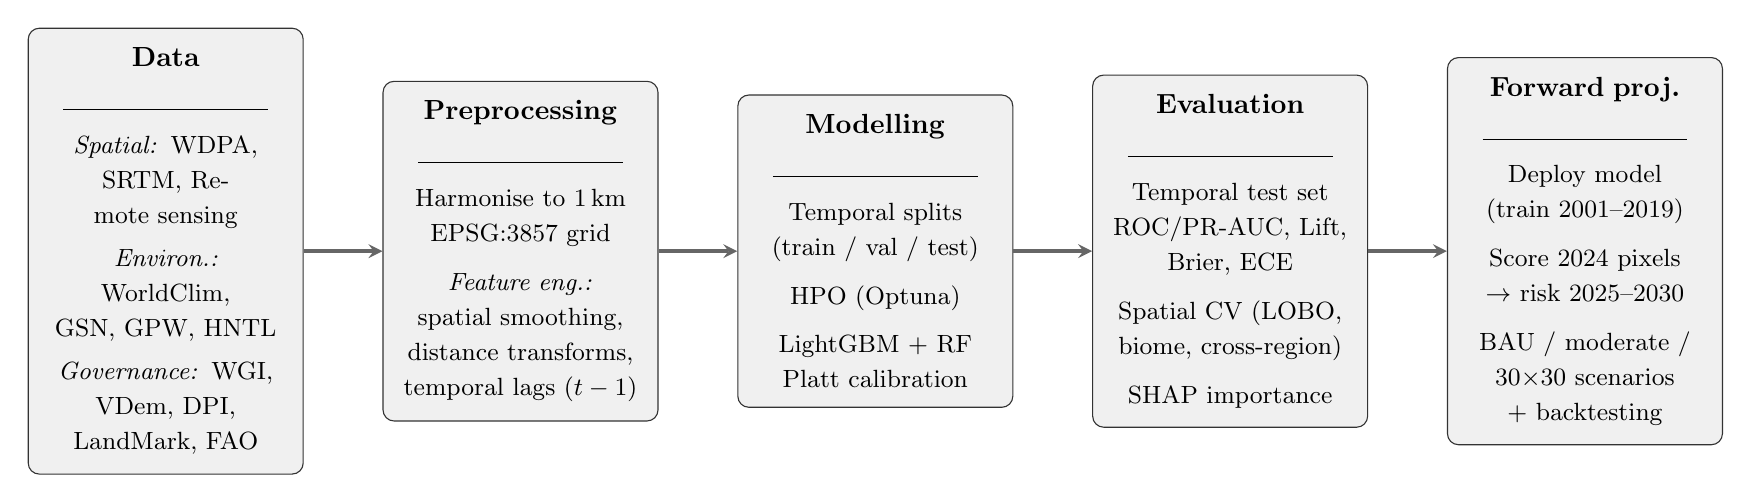
\begin{tikzpicture}[
  node distance = 0.35cm and 1.0cm,
  stage/.style  = {rectangle, rounded corners=4pt, draw=black!80, fill=gray!12,
                   text width=3.0cm, align=center, font=\small\linespread{1.15}\selectfont,
                   inner sep=7pt, minimum height=2.6cm},
  stageH/.style = {stage, fill=blue!8},
  arrow/.style  = {->, >=stealth, very thick, draw=black!60}
]

\node[stage]  (data)  {{\normalsize\textbf{Data}}\\[3pt]
                        \rule{2.6cm}{0.3pt}\\[3pt]
                        \textit{Spatial:} WDPA,\\ SRTM, Remote sensing\\[3pt]
                        \textit{Environ.:} WorldClim,\\ GSN, GPW, HNTL\\[3pt]
                        \textit{Governance:} WGI,\\ VDem, DPI,\\ LandMark, FAO};

\node[stage, right=of data]  (prep)  {{\normalsize\textbf{Preprocessing}}\\[3pt]
                        \rule{2.6cm}{0.3pt}\\[3pt]
                        Harmonise to 1\,km\\ EPSG:3857 grid\\[5pt]
                        \textit{Feature eng.:}\\
                        spatial smoothing,\\ distance transforms,\\ temporal lags ($t-1$)};

\node[stage, right=of prep]  (model) {{\normalsize\textbf{Modelling}}\\[3pt]
                        \rule{2.6cm}{0.3pt}\\[3pt]
                        Temporal splits\\
                        (train / val / test)\\[5pt]
                        HPO (Optuna)\\[5pt]
                        LightGBM + RF\\ Platt calibration};

\node[stage, right=of model] (eval)  {{\normalsize\textbf{Evaluation}}\\[3pt]
                        \rule{2.6cm}{0.3pt}\\[3pt]
                        Temporal test set\\ ROC/PR-AUC, Lift,\\ Brier, ECE\\[5pt]
                        Spatial CV (LOBO,\\ biome, cross-region)\\[5pt]
                        SHAP importance};

\node[stage, right=of eval]  (fwd)   {{\normalsize\textbf{Forward proj.}}\\[3pt]
                        \rule{2.6cm}{0.3pt}\\[3pt]
                        Deploy model\\ (train 2001--2019)\\[5pt]
                        Score 2024 pixels\\ $\to$ risk 2025--2030\\[5pt]
                        BAU / moderate /\\ 30$\times$30 scenarios\\ + backtesting};

\draw[arrow] (data)  -- (prep);
\draw[arrow] (prep)  -- (model);
\draw[arrow] (model) -- (eval);
\draw[arrow] (eval)  -- (fwd);

\end{tikzpicture}
}
\vspace{3pt}
\caption{End-to-end pipeline overview.}
\label{fig:pipeline}
\end{figure}

% ---------------------------------------------------------------------------
\label{sec:preprocessing}
\paragraph{Reprojection and resampling.}
Every input raster is reprojected to the common 1~km backbone grid and temporally
aligned to calendar years. For continuous variables (elevation, NDVI, climate, night-time lights), bilinear
interpolation is used during reprojection. For population density (a count-based
variable), bilinear interpolation is also applied, consistent with GPW's own
resampling guidance; the resulting values are continuous estimates of population
per km$^2$, appropriate for tree-based models. For categorical and binary layers
(land-cover class, PA status, conservation priority indicators), nearest-neighbour
interpolation preserves discrete class boundaries; area-fraction resampling was
not used to avoid artificially diluting binary indicators. Satellite image collections with
multiple acquisitions per year are collapsed to a single annual summary: annual median
for continuous variables (reducing cloud contamination and sensor noise) and cumulative
sum for fire events (accumulating burned area over the year).

\paragraph{Panel assembly.}
Following reprojection and temporal alignment, all layers are merged into a unified
pixel--year panel. Each row corresponds to a single grid cell $i$ observed in year $t$
and contains the binary target variable $\text{transition}_{i,t}$ (defined formally
in Section~\ref{sec:framework}), the full set of static and dynamic predictor
variables, and cell and year identifiers. The South America panel contains
approximately 413~million pixel--year observations across 20.8~million unique grid
cells over 25 annual periods (2000--2024); comparable panels are constructed for the
United States and Southeast Asia.

% ---------------------------------------------------------------------------
\subsection{Modelling Framework}
\label{sec:framework}

\paragraph{Problem formulation.}
The objective is to estimate, for each currently unprotected 1~km$^2$ grid cell $i$
observed in year $t$, the probability that cell $i$ becomes newly designated as a
protected area within the subsequent five years. Let $y_{i,t} \in \{0,1\}$ denote
whether cell $i$ is protected in year $t$. The target variable is a five-year
forward-looking binary indicator:
A single PA designation can create positive labels for the same cell across multiple
overlapping five-year windows (e.g.\ a cell that transitions in 2015 generates
positives for observations at $t = 2010, 2011, \ldots, 2014$). This within-cell
label duplication creates positive autocorrelation across time but does not constitute
leakage because all labels are constructed looking \emph{forward} from year $t$ and
no future PA information enters the feature vector. Standard pixel--year metrics such
as PR-AUC treat each row independently; the event-level recall metric
(Section~\ref{sec:results_sa_events}) removes this duplication by counting each
unique PA polygon once.
\begin{equation}
  \text{transition}_{i,t} =
  \begin{cases}
    1 & \text{if } y_{i,t} = 0 \text{ and } y_{i,t+k} = 1
        \text{ for any } k \in \{1,\dots,5\}, \\
    0 & \text{otherwise.}
  \end{cases}
  \label{eq:target}
\end{equation}
A five-year horizon is chosen for three reasons: it aligns the forecast horizon
directly with the 2025--2030 window of the 30$\times$30 target; it absorbs gazette-date
recording lags of one to three years without censoring true designation events; and it
provides a large enough positive class per observation year to support reliable model
training despite rare-event class imbalance.

\paragraph{Risk set and right-censoring.}
Only unprotected pixels ($y_{i,t} = 0$) are eligible for the transition and therefore
included in the analysis. Once a pixel becomes protected, it exits the risk set
permanently and does not contribute further observations. This prevents the model from
learning to predict non-events for land that is already protected.

Right-censoring is a technical constraint arising from the finite data horizon.
To observe the full five-year outcome window, the last year for which a label can be
constructed is 2019 (using PA designations through 2024). All pixel--year observations
beyond 2019 are excluded from model training and evaluation; the target variable is
undefined for them because we cannot verify whether a transition occurs in the full
subsequent five-year window. This cutoff year is denoted \texttt{LAST\_LABEL\_YEAR}~$= 2019$.

\paragraph{Rare-event structure.}
Transitions into protected status are rare: fewer than 0.5\% of eligible pixel--year
observations record a positive outcome. This extreme class imbalance is not an
artefact of data collection but reflects the true pace of PA expansion relative to
the vast unprotected land area. Standard classifiers trained on such data tend to
predict the majority class (non-transition) for almost all observations and achieve
high nominal accuracy while being useless for identifying future designations \citep{davis2006}.
The modelling choices described in Sections~\ref{sec:models}--\ref{sec:splits}
are designed specifically to address this challenge.

\paragraph{Relation to discrete-time hazard models.}
The panel formulation of Equation~(\ref{eq:target}) is conceptually related to
discrete-time hazard (or duration) models used in econometrics to study the timing
of events such as unemployment spells, technology adoption, or firm bankruptcy
\citep{allison1982, singer1993}.
In the hazard interpretation, each unprotected pixel is ``at risk'' of designation
in each year, and the model estimates the conditional probability of transitioning
given that no transition has occurred yet. Unlike parametric hazard models, the
tree-based machine-learning approach used here imposes no functional form on the
relationship between predictors and the transition probability, and handles complex
interactions among the 73 engineered covariates without prior specification.
Unlike a parametric hazard model, the target here is a \emph{five-year cumulative}
transition indicator with overlapping windows; the output probabilities should be
interpreted as five-year cumulative designation risks, not annual conditional hazards.

\paragraph{Prediction, not prescription.}
The framework learns \emph{where governments have historically designated} PAs and
extrapolates this pattern forward. It does not predict where PAs \emph{should} be
designated for maximum conservation impact. The two questions have different answers because real designation is not only shaped
by biodiversity optimisation, but also by political feasibility and opportunity cost \citep{schuster2023}. The gap between predicted and optimal designations is itself
a substantive finding discussed in Section~\ref{sec:discussion}.

% ---------------------------------------------------------------------------
\subsection{Feature Engineering}
\label{sec:features}

Raw cell-level features describe conditions at a single pixel. Because PA designation
is influenced by conditions in the surrounding landscape, additional features are engineered to encode spatial
context at multiple scales.

\paragraph{Multi-scale spatial smoothing.}
For a selected subset of time-varying predictors (NDVI, population density, night-time
lights, deforestation intensity, and wildfire), uniform averaging kernels of size
$4 \times 4$, $16 \times 16$, and $64 \times 64$ grid cells are applied, corresponding
to neighbourhood extents of 4~km, 16~km, and 64~km respectively. These three scales are designed to capture: (i) immediate local context (4~km: adjacent land use, buffer
zones); (ii) sub-regional landscape dynamics (16~km: agricultural frontier gradients,
infrastructure corridors); and (iii) landscape-scale patterns (64~km: macro-regional
biome boundaries, large-scale deforestation fronts). Including all three scales allows
the model to select the most informative spatial context for each combination of
predictor and location without imposing a single fixed neighbourhood size
\citep{collart2025, mcgarigal2016}.

\paragraph{Distance-based features.}
In addition to smoothed averages, Euclidean distances to the nearest PA boundary,
road segment, power plant, and oil and gas installation are included as features.
Distances are computed in EPSG:3857 and therefore slightly overstate ground distances
at higher latitudes; for South America and Southeast Asia (predominantly within
$\pm 30^\circ$) the overstatement is below 15\%, which does not affect the rank
ordering used by tree splits.
These distance measures directly encode proximity to conservation and development
infrastructure, capturing processes such as incremental PA network expansion and
the deterrent effect of industrial activity on designation.

\paragraph{Temporal lag.}
All time-varying features, including the distance to existing PAs, are lagged by
one year: features at year $t$ reflect conditions recorded through end of year $t-1$.
This ensures that the model cannot use information about PAs designated in year $t$
itself to predict the transition target for year $t$, which would constitute temporal
leakage. For example, distance to the nearest PA at year $t$ is computed using only
the PA network as it stood at end of year $t-1$, so designation events in year $t$ do
not inform the features used to predict those same events.

% ---------------------------------------------------------------------------
\subsection{Models and Calibration}
\label{sec:models}

Three modelling approaches are estimated for each region, in increasing order of
complexity.

\paragraph{Static Suitability Baseline.}
A static suitability model is estimated on cross-sectional data from the year 2000:
it learns to distinguish pixels that are already protected from those that are not,
using only time-invariant geographic characteristics (elevation, biodiversity, climate,
remoteness). Scores for the unprotected year-2000 pixels are then compared against PA
designations observed between 2000 and 2024. Because this model ignores all temporal
dynamics and uses a different target (current protection status rather than future
transition), it establishes a meaningful benchmark: any gain over the static baseline
quantifies the added value of temporal variation in covariates and the transition-specific
training setup.

\paragraph{Random Forest.}
A Random Forest \citep{breiman2001} classifier is trained on the pixel--year panel.
The algorithm builds an ensemble of 300 decision trees, each fitted to an independent
bootstrap sample of the data, considering a random subset of features at every split.
Predictions are obtained by averaging probabilities across all trees. This
ensemble structure produces probability estimates that are more stable than any
single tree and naturally provides feature importance measures from the average
reduction in node impurity across splits. Class imbalance is handled via
\texttt{class\_weight="balanced\_subsample"}, which reweights minority-class
(transition) observations within each tree in inverse proportion to their frequency.

\paragraph{LightGBM.}
Light Gradient-Boosting Machine (LightGBM; \citealp{ke2017}) is the primary reporting
model throughout the analysis. Both LightGBM and Random Forest are fully trained and
evaluated production models; results are reported for LightGBM by default because it
attains superior performance on the calibration-sensitive metrics most relevant for
transition-risk applications (PR-AUC and Brier score), while RF results serve as
confirmation. Section~\ref{sec:results_sa_metrics} elaborates on this choice.

Gradient boosting builds an ensemble of decision trees sequentially: each tree is
fitted to the negative gradient (pseudo-residuals) of the ensemble's current loss,
so successive trees progressively correct prediction errors. LightGBM introduces
Gradient-based One-Side Sampling (GOSS), which retains all large-gradient observations
and subsamples low-gradient ones, and Exclusive Feature Bundling (EFB), which groups
mutually exclusive sparse features. These optimisations make it substantially faster
than standard gradient boosting on large datasets with accuracy competitive with XGBoost across standard benchmarks \citep{ke2017}, a critical
advantage for panels of 100--350 million observations.
 Class imbalance is handled via
\texttt{scale\_pos\_weight}, set equal to the ratio of negative to positive
observations in the training set:
\begin{equation}
  \texttt{scale\_pos\_weight} = \frac{N_{\text{neg}}}{N_{\text{pos}}}.
  \label{eq:spw}
\end{equation}
This upweights each minority-class (transition) observation in the binary cross-entropy
loss, steering the boosting iterations toward correct identification of rare designations.
The parameter is recomputed from the training data for each model run and is not tuned
as a hyperparameter.

Hyperparameters for both models are selected via Bayesian optimisation using
Optuna \citep{akiba2019} with a TPE sampler and median pruner, running up to
100~trials per region. The optimisation objective is PR-AUC on the held-out
early-stopping split of the innermost cross-validation fold (see Section~\ref{sec:splits}).
Table~\ref{tab:hyperparams} reports the key fixed and tuned values; the Optuna TPE
search used random seed 42 with in-memory storage (no distributed backend). The
search space for LightGBM covers: \texttt{num\_leaves} $\in [20, 300]$,
\texttt{learning\_rate} $\in [0.01, 0.3]$ (log-scale), \texttt{min\_child\_samples}
$\in [20, 200]$, \texttt{subsample} $\in [0.5, 1.0]$, \texttt{colsample\_bytree}
$\in [0.5, 1.0]$, \texttt{reg\_alpha}/\texttt{reg\_lambda} $\in [10^{-3}, 10]$
(log-scale). The number of boosting rounds is determined by early stopping
(patience 500 rounds, metric PR-AUC on the fold early-stop split) within each HPO
trial; the final production model uses the training-size-weighted average of
fold-level best iterations (see Section~\ref{sec:splits}).
%TODO: NEEDS COMPUTATION: report final selected hyperparameter values per region/model in a supplementary table before submission.

\begin{table}[H]
\centering
\caption{Key hyperparameter values for the Random Forest (RF) and LightGBM (LGBM)
transition models.}
\label{tab:hyperparams}
\small
\begin{tabular}{llll}
\toprule
\textbf{Parameter} & \textbf{RF} & \textbf{LightGBM} & \textbf{Notes} \\
\midrule
Trees / rounds & 300 & Tuned per region & Fixed from CV \\
Max depth & Unlimited & Tuned & LGBM: $-1$ = no limit \\
Min samples per leaf & 1 & Tuned & LGBM: \texttt{min\_child\_samples} \\
Class imbalance & \texttt{balanced\_subsample} & \texttt{scale\_pos\_weight} & See Eq.~(\ref{eq:spw}) \\
Random seed & 42 & 42 & Fixed for reproducibility \\
\bottomrule
\end{tabular}
\end{table}

% ---------------------------------------------------------------------------
\paragraph{Probability Calibration.}
\label{sec:calibration}

Raw model outputs are scores, not calibrated probabilities. A raw score of 0.7 does
not mean the pixel has a 70\% chance of being designated; it only indicates that the
pixel ranks above most others in the predicted risk distribution. This distinction
is consequential for transition-risk applications: portfolio screening or regulatory
stress-testing requires not just a ranking of risky assets but also an estimate of
\emph{how risky}, expressed as a probability that admits direct comparison across
assets and thresholds.

The gap between raw scores and true probabilities arises because the class-weighting
scheme (Equation~\ref{eq:spw}) reshapes the effective class distribution seen by the
model. After reweighting, the model optimises against a balanced distribution and
learns to assign higher scores than the true probability of the minority class warrants.

To correct this, calibration is performed using Platt scaling \citep{platt1999,
niculescumizil2005}: a logistic regression is fitted with the raw model scores as
input and the true binary labels as the outcome, using out-of-fold cross-validation
predictions so that no test-set information enters the calibration. This logistic function maps raw scores to calibrated probabilities with improved
alignment to observed transition rates across score bands. Platt scaling is not
guaranteed to achieve perfect calibration in every quantile, particularly in the
high-risk tail where sample sizes are small; ECE is therefore supplemented by
reliability diagrams (Appendix~\ref{app:calibration}) that allow visual inspection
of calibration quality at the top 1--5\% of the score distribution. Isotonic regression
\citep{zadrozny2002} is computed as a robustness check. Calibrated probabilities are
clipped to $(10^{-6},\, 1 - 10^{-6})$ for numerical stability. All probability maps
and risk scores reported in this thesis use Platt-calibrated predictions.

% ---------------------------------------------------------------------------
\subsection{Training, Validation, and Test Design}
\label{sec:splits}

\paragraph{Temporal splits.}
Model training and evaluation strictly preserve temporal order to ensure that all
reported metrics reflect the model's ability to forecast \emph{future} designations
using only \emph{past} information. The training design consists of three stages:

\textbf{Hyperparameter optimisation (Optuna HPO).}
Optuna \citep{akiba2019} runs up to 100~trials, each fitting LightGBM or Random
Forest with a candidate hyperparameter configuration and evaluating PR-AUC on the
held-out early-stopping split within three expanding-window temporal cross-validation
folds:
\begin{itemize}
  \item Fold 1: train 2001--2008, early-stop validation 2009--2011.
  \item Fold 2: train 2001--2011, early-stop validation 2012--2013.
  \item Fold 3: train 2001--2013, early-stop validation 2014--2016.
\end{itemize}
Year 2000 is excluded from all folds: the WDPA records it as a cross-sectional
baseline in which all pre-existing PAs appear as newly designated, not as true annual
transition events. The best hyperparameter set is selected based on average
out-of-fold PR-AUC across the three folds.

\textbf{Final evaluation model.}
Using the selected hyperparameters, a final LightGBM model is trained on all
non-test-period data (2001--2016). During each CV fold, early stopping (patience 500
rounds) was used to find the number of boosting rounds that maximises PR-AUC on the
fold's early-stop split; the final model trains for a fixed number of rounds equal to
the training-size-weighted average of these fold-level best iterations, scaled by 1.05
to account for the larger effective training set, and no lower than the best iteration
of the longest fold (Fold~3). This procedure determines training depth without
exposing the test period.

\textbf{Test period.}
The test set covers 2017--2019, held out entirely throughout hyperparameter search and
model fitting. The upper boundary 2019 coincides with \texttt{LAST\_LABEL\_YEAR}: all
pixel--year observations from 2020 onwards are right-censored. Every metric reported
in Section~\ref{sec:results} is an out-of-sample estimate based on this held-out
test period. The temporal test is future-out-of-sample but not location-out-of-sample:
the same pixel (once it exits the risk set upon designation) can appear in both
training and test years. Static covariates (elevation, climate, GSN layers) are
identical across years for the same pixel, which could contribute to optimistic
performance estimates. The LOBO evaluation addresses this by withholding entire
biomes, providing a stricter spatial generalisation test.

\paragraph{Leakage prevention.}
Multiple safeguards prevent future information from reaching the model. (i) All
time-varying features are lagged by one year, so the covariate vector at year $t$
reflects conditions recorded through end of year $t-1$ (Section~\ref{sec:features}).
(ii) Distance to existing PAs is computed using only the PA network as of year $t-1$,
so same-year designation events cannot leak into the distance feature for that year.
(iii) Hyperparameters are tuned using the Optuna HPO procedure described above, whose
CV folds do not touch the test period; the test set is never used to guide any
modelling decision. (iv) Probability calibrators are fitted exclusively on out-of-fold
predictions generated during the CV folds, not on test data.

\paragraph{Temporal sample weighting.}
Conservation-policy dynamics evolve over time, and recent designation patterns are
more informative for forecasting the near future than patterns from two decades ago.
Training observations are therefore assigned a linearly increasing sample weight:
year 2001 receives weight 0.5 and the last training year receives weight 1.0, with
all intermediate years interpolated proportionally. This places greater emphasis on
recent patterns while retaining the full historical record. The 0.5 floor is a modelling
choice; sensitivity to this value (e.g.\ uniform weights or a steeper ramp) has not
been formally tested but is not expected to substantially alter rankings given the
smoothly varying nature of policy drivers.

\paragraph{Class imbalance handling.}
Transitions are rare ($\approx 0.3$--$0.5\%$ of eligible pixel--year observations).
No oversampling or undersampling is applied; the empirical frequency is preserved.
Instead, class weights (LightGBM: \texttt{scale\_pos\_weight}; Random Forest:
\texttt{balanced\_subsample}) adjust the contribution of minority-class observations
to the loss function. This approach avoids distorting the spatial or temporal
structure of the data.

\paragraph{Reproducibility.}
All random components (tree construction, bootstrap sampling, Optuna trial
initialisation) are controlled via a fixed random seed (42 throughout). The full
pipeline is implemented in Python~3.12 using scikit-learn~1.4, LightGBM~4.3
\citep{ke2017,pedregosa2011}, and GeoPandas~0.14, with intermediate outputs stored in
Apache Parquet format for efficient column-oriented access. Large-scale model training
(involving panels of 100--350 million rows) is executed on the ETH Zurich Euler
high-performance computing cluster. Jobs are submitted as SLURM array tasks.
Key library versions, data release dates, and SLURM job templates are recorded in the
repository's \texttt{environment.yml} and \texttt{data\_provenance.csv};
together with the fixed seed these constitute the reproducibility artefacts for the
main evaluation results.
%TODO: NEEDS COMPUTATION: pin exact LightGBM/scikit-learn patch versions and record git commit hash before final submission.

% ---------------------------------------------------------------------------
\subsection{Evaluation}
\label{sec:metrics}

Because the positive class constitutes fewer than 0.5\% of observations, accuracy-based
metrics (e.g.\ overall accuracy, $F_1$-score) are uninformative: a model that predicts
zero transitions everywhere achieves $> 99.5\%$ accuracy \citep{davis2006}. Evaluation
therefore focuses on metrics that are robust to severe class imbalance and that
directly reflect the ranking quality of predicted risks.

\paragraph{Precision--Recall AUC (PR-AUC).}
The primary metric. The precision--recall curve plots precision (fraction of top-ranked
pixels that actually transition) against recall (fraction of all transitions captured)
as the classification threshold is varied:
\begin{align}
  \text{Precision}(k) &= \frac{TP(k)}{TP(k) + FP(k)}, \quad
  \text{Recall}(k) = \frac{TP(k)}{TP(k) + FN(k)}.
\end{align}
Here $TP(k)$, $FP(k)$, and $FN(k)$ denote true positives, false positives, and false
negatives at threshold $k$. PR-AUC is computed as scikit-learn's \texttt{average\_precision\_score}, which uses
the step-function (interpolation-free) approximation rather than trapezoidal integration.
Under severe class imbalance, PR-AUC is a more informative summary of discriminative
performance than ROC-AUC because it places weight on the model's ability to correctly
rank positive observations at the top of the score distribution \citep{davis2006}.

\paragraph{ROC-AUC.}
ROC-AUC measures the probability that a randomly chosen positive observation receives
a higher predicted score than a randomly chosen negative. A value of 0.5 corresponds
to random ranking and 1.0 to perfect discrimination. Although ROC-AUC is less
sensitive than PR-AUC under extreme class imbalance, since it is dominated by the large
number of true negatives; it provides a useful reference point for comparing model
quality across settings with different base rates and for detecting degenerate or
anti-predictive models.

\paragraph{Precision at top-$k$\% and lift.}
For policy use, the most relevant question is: ``if I inspect the top $k$\% of
predicted-risk pixels, what fraction will actually be designated?'' This is precision
at top $k$\% of the score distribution ($P@k\%$). To account for differences in
base rates across evaluation splits, we also report \emph{lift}:
\begin{equation}
  \text{Lift}@k\% = \frac{P@k\%}{\text{baseline positive rate}}.
\end{equation}
A lift of 60 at the top 1\% means that screening the top 1\% of pixels yields 60
times more future designations per unit area than random selection. Lift is reported
at $k \in \{1, 5, 10\}$.

\paragraph{Brier score.}
The mean squared error of calibrated predicted probabilities:
\begin{equation}
  \text{Brier} = \frac{1}{N} \sum_{i,t} \bigl(\hat{p}_{i,t} - y_{i,t}\bigr)^2.
\end{equation}
A lower Brier score indicates better-calibrated and more accurate probability
estimates. The Brier score is bounded between 0 (perfect) and 1 (maximally wrong).
Under a positive rate of $\pi$, a naive model that predicts the base rate
$\hat{p} = \pi$ everywhere achieves a Brier score of $\pi(1-\pi)$, which for
$\pi \approx 0.008$ equals approximately $0.0079$. A well-fitted model must beat this threshold; for the South America model with
$\pi \approx 0.008$, the no-information baseline is approximately~0.0079, and the
calibrated LightGBM Brier score of 0.00421 represents a nearly 50\% reduction
(see Table~\ref{tab:sa_metrics} for per-region baselines).

\paragraph{Expected Calibration Error (ECE).}
ECE measures the average discrepancy between predicted probabilities and observed
frequencies, computed by binning predictions into equal-width intervals and comparing
the average predicted probability to the observed transition rate within each bin:
\begin{equation}
  \text{ECE} = \sum_{b=1}^{B} \frac{|n_b|}{N}
    \left| \overline{p}_b - \overline{y}_b \right|,
\end{equation}
where $n_b$ is the number of observations in bin $b$, $\overline{p}_b$ is their
mean predicted probability, and $\overline{y}_b$ is their observed transition rate.
ECE is computed both before and after Platt scaling to directly quantify the
calibration improvement achieved by post-hoc recalibration \citep{niculescumizil2005}.
A lower ECE indicates that predicted probabilities more faithfully track observed
transition rates across the full range of predicted scores.

% ---------------------------------------------------------------------------
\paragraph{Feature Importance (SHAP).}
\label{sec:shap_methods}

To explain which features drive individual predictions, SHapley Additive exPlanations
(SHAP; \citealp{lundberg2017}) are computed for the LightGBM model using the
tree-explainer algorithm. SHAP values are grounded in cooperative game theory:
for each observation, the SHAP value of a feature equals its average marginal
contribution to the model's output across all possible orderings in which features
could be introduced. A positive SHAP value for a given pixel--feature pair indicates
that the feature's value at that pixel pushes the predicted probability above the
mean; a negative value indicates suppression of risk. The mean absolute SHAP value
across all test-set observations is used to rank features by their average
contribution to model predictions. This analysis is computed on the temporal test set (2017--2019). The TreeSHAP
algorithm explains the raw LightGBM log-odds output (before Platt scaling); since
Platt scaling is a monotone transformation, the SHAP-derived feature ranking and
directional effects are preserved under calibration, though the magnitude of SHAP
values reflects the log-odds scale, not the calibrated probability scale. This is
separate from the feature importance computed during Optuna HPO (which uses impurity-based importance
from the CV folds). Using the held-out test set for SHAP analysis is appropriate
because it is the same data used to compute all reported benchmark metrics,
so the feature attributions reflect model behaviour under genuine out-of-sample
conditions without introducing any additional leakage beyond what is already
present in the evaluation design.

% ---------------------------------------------------------------------------
\subsection{Spatial Robustness Evaluation}
\label{sec:spatial_cv}

In addition to temporal out-of-sample evaluation, spatial robustness is assessed
through a three-layer framework that tests whether the model's predictive patterns
hold across geographic settings it was not explicitly trained on \citep{ploton2020}.

\subsubsection{Leave-One-Biome-Out (LOBO)}
\label{sec:lobo}
LOBO cross-validation, adapted from spatial leave-one-group-out procedures
\citep{ploton2020, roberts2017}, provides the strictest within-continent
generalisation test. Biomes are defined using the WWF terrestrial ecoregion
classification from the Global Safety Net (GSN) layer. For each biome $b$, a
separate model is trained on all observations from all \emph{other} biomes and
evaluated on the held-out biome's test-period pixels. A biome with low LOBO performance indicates that its designation patterns are
structurally different from those in the rest of the continent. LOBO is the strictest
within-continent spatial evaluation implemented in this thesis; note that it retains
the same countries, neighbouring ecoregions, and broad continental gradients in
training, so it is not equivalent to leave-country-out or spatial-block CV, which
would provide stricter geographic separation.

PR-AUC is reported as the primary LOBO metric because it is more informative
than ROC-AUC under the extreme class imbalance typical of held-out biomes.
Since each biome has a different positive rate, raw PR-AUC values are not
directly comparable across biomes: a biome where 10\% of pixels receive
designation has a random-classifier PR-AUC of~0.10, while one where only
0.1\% receive designation has a random-classifier PR-AUC of~0.001. To enable
cross-biome comparison, results are therefore also expressed as
\emph{PR-AUC lift}---the ratio of the observed PR-AUC to the biome's positive
rate. A lift of~1 indicates performance indistinguishable from a random
classifier; values above~1 indicate genuine predictive signal above the naive
baseline. Raw PR-AUC values are reported alongside lift in the appendix tables
for completeness.

\subsubsection{Biome-Stratified Evaluation}
\label{sec:cv2}
The standard (full-data) production model is scored on the test period, and its
performance metrics are broken down by biome. Unlike LOBO, this diagnostic does not
test generalisation to unseen biomes: the model was trained on all biomes
simultaneously. Instead, it reveals where within a continent the model performs
well or poorly, specifically which biomes produce the clearest predictive signal versus where
prediction is harder even when the biome's own history was available for training.
This biome-level performance map is useful for communicating the reliability of
risk scores in specific geographic areas.

\subsubsection{Cross-Continental Transfer}
\label{sec:cv3}
Cross-continental transfer provides the most demanding spatial test: a model trained
on one continent is scored on another without any retraining. Transfer is performed
in all six directions (SA$\to$USA, USA$\to$SA, SA$\to$SEA, USA$\to$SEA,
SEA$\to$SA, SEA$\to$USA) using the common feature set available in all three
regions. High transfer performance would imply that the model has learned universal
ecological and governance drivers of PA designation. Near-random transfer performance could reflect genuine institutional specificity of
designation patterns, but several technical explanations should also be considered:
inconsistent categorical feature distributions across regions (land-cover codes,
ecoregion codes), covariate distribution shift, different base rates causing
calibration mismatch, or model overfitting to region-specific correlational patterns.
The cross-continental transfer results should therefore be interpreted as an upper
bound on institutional specificity rather than direct evidence of it.

% ---------------------------------------------------------------------------
\subsection{Forward Prediction to 2030}
\label{sec:forward}

\paragraph{Deployment model.}
The forward prediction setup is identical to the evaluation model in every respect,
using the same hyperparameters, same features, same class-weighting scheme, and same
Platt calibration procedure, with one difference: the training window is extended
to include all non-censored years. A deployment model is therefore trained on
2001--2019 (all years for which the five-year transition target can be constructed
without right-censoring), using the same hyperparameter configuration selected by
the Optuna HPO stage and the same number of boosting rounds as the evaluation model.
Because the deployment model trains on all labeled data including the 2017--2019
test period, no held-out set is available for calibration. An auxiliary model trained
on 2001--2016 is therefore used to score 2017--2019 as a held-out proxy, and the
resulting out-of-fold predictions are used to fit the Platt and isotonic calibrators.
This is a practical approximation: the calibrator is fitted on the 2017--2019 proxy
period rather than as a true out-of-fold estimate for the 2001--2019 deployment model.
The resulting calibration mismatch is expected to be small because the proxy period
immediately precedes the deployment period; backtesting (Appendix~\ref{app:backtest})
confirms that precision@1\% is stable across historical origins, providing indirect
evidence that calibration quality is maintained.

\paragraph{Forward inference.}
Inference is performed on the 2024 covariate snapshot for all pixels unprotected as
of 2023. The deployment model assigns each candidate pixel a calibrated five-year
cumulative probability of becoming protected between 2025 and 2030. The information
set is as follows: model training uses PA outcomes through 2019
(\texttt{LAST\_LABEL\_YEAR}); the deployment training set includes labels whose
five-year windows extend through 2024, which is acceptable for a forecast made at
the start of 2025. No 2024 covariate or PA-boundary information enters the feature
vector used for inference. On temporal
alignment: all time-varying features are lagged by one year (Section~\ref{sec:features}),
so the 2024 covariate snapshot reflects conditions recorded through end-2023.
Since unprotected status is evaluated at end-2023 (``unprotected as of 2023''),
the effective reference date for the five-year lookahead is the beginning of 2025,
placing the forecast horizon squarely within the 2025--2030 window of the 30$\times$30
target.

\paragraph{Policy scenarios.}
Three scenarios are derived from the resulting probability surface by varying the
cumulative area designated:
\begin{itemize}
  \item \textbf{Business-as-usual (BAU):} cumulative new area equals the observed
    2019--2024 designation volume, projecting the recent empirical designation rate
    forward.
  \item \textbf{Moderate:} cumulative area targets the midpoint between each
    region's current coverage and 30\%, applied proportionally.
  \item \textbf{30$\times$30:} cumulative area targets full 30\% terrestrial
    coverage by 2030.
\end{itemize}
Under each scenario, pixels are ranked by their calibrated probability and the
highest-probability pixels are selected until the cumulative area target is reached,
producing spatially explicit allocation maps. These are deterministic allocation
scenarios, not stochastic simulations: they identify \emph{where} historical-pattern
extrapolation would place new PAs, but do not model uncertainty in individual
outcomes, political or legal feasibility constraints, contiguity requirements, or
tenure restrictions. They should be read as risk-concentration maps, not forecasts
of which specific parcels will be designated. Hotspot clusters are identified via
spatial clustering \citep{ester1996} on the top-probability pixels.

\paragraph{Backtesting.}
Methodological validity is established by backtesting: pseudo-forecasts are generated
at historical origins $T \in \{2009, 2011\}$, each time training on 2001--$(T-1)$,
scoring unprotected pixels in year $T$, and evaluating against realised designations
in years $T+1$ through $T+5$. False-positive maps are also computed for $T=2017$ using
the evaluation model (trained on 2001--2016), which is distinct from the two walk-forward
backtest origins above; this is labelled clearly in Appendix~\ref{app:backtest}.
This walk-forward evaluation empirically verifies that the forward deployment procedure
generalises to out-of-sample designation events.

% ===========================================================================
%  Results
% ===========================================================================
\section{Results}
\label{sec:results}

% ---------------------------------------------------------------------------
\subsection{South America: Model Performance}
\label{sec:results_sa}
\label{sec:descriptive}

The South America panel contains approximately 413~million pixel--year observations
spanning 20.8~million unique 1~km$^2$ grid cells over 25 annual periods (2000--2024).
By 2024, 25.6\% of South America's terrestrial area is formally protected under WDPA,
up from approximately 15\% in 2000 (formal PAs only; OECMs excluded). All coverage
percentages are computed using equal-area pixel counts (see Section~\ref{sec:harmonisation}).
As a consequence of this cumulative expansion, the risk set shrinks from roughly
20.8~million eligible pixels in 2000 to approximately 15.7~million by the end of the sample.

Transitions from unprotected to protected status are rare events. The average
transition rate across the full South America panel is approximately 0.5--0.8\%
per pixel--year, implying that a given pixel has less than a 1-in-100 chance of
being designated in any given year. This rate is not constant over time: designation
rates were higher during 2000--2013, a period of active PA expansion in the Amazon
and Cerrado, and declined thereafter. In the held-out test period (2017--2019), 380,064 transitions occur among approximately
47.7~million eligible pixel--year observations, corresponding to a positive rate of
approximately 0.8\%. Pixel--year observations are spatially and temporally
autocorrelated; headline metrics should be interpreted as point estimates without
formal confidence intervals, with the LOBO and cross-regional evaluations providing
a practical range of spatial generalisation performance.

The United States panel covers approximately 200~million pixel--year observations.
Current protection stands at 7.7\%, and the test-period transition rate is
approximately 0.04\% (an order of magnitude lower than South America), reflecting
the US's severely constrained designation pace relative to its 30\% target. Southeast
Asia covers approximately 100~million pixel--year observations, with current PA
coverage of 14.0\% and a test-period transition rate of approximately 0.6\%.

These patterns reflect three defining features of the data: (i) a large risk set;
(ii) strong temporal heterogeneity in transition rates across regions and time periods;
and (iii) extreme class imbalance, most pronounced in the US and in later sample years.

% ---------------------------------------------------------------------------
\subsubsection{Discrimination Metrics}
\label{sec:results_sa_metrics}

Table~\ref{tab:sa_metrics} reports temporal test-set performance for the LightGBM
and Random Forest transition models applied to South America (test period: 2017--2019).
Lift@$k$\% equals Precision@$k$\% divided by the baseline positive rate; since
Recall@$k$\% = Lift@$k$\% $\times$ $k$\% (for a uniform test distribution), the
pixel-year Recall@1\% can be read as $66.8\% \approx 66.8 \times 0.01$ for LGBM.
Event-level recall (77.4\%; Section~\ref{sec:results_sa_events}) differs because
it deduplicates overlapping five-year windows.

\begin{table}[H]
\centering
\caption{Predictive performance on the temporal test set (2017--2019) for South
America. Baseline positive rate: 0.797\%.}
\label{tab:sa_metrics}
\begin{tabular}{lcc}
\toprule
\textbf{Metric} & \textbf{LightGBM} & \textbf{Random Forest} \\
\midrule
ROC-AUC              & 0.897  & 0.927 \\
PR-AUC               & 0.645  & 0.634 \\
Precision @ top 1\%  & 0.532  & 0.539 \\
Lift @ top 1\%       & 66.8$\times$ & 67.6$\times$ \\
Precision @ top 5\%  & 0.116  & 0.121 \\
Lift @ top 5\%       & 14.5$\times$ & 15.2$\times$ \\
Brier score          & 0.00421 & 0.00458 \\
ECE (post-calibration) & 0.0081 & 0.0109 \\
\bottomrule
\end{tabular}
\end{table}
The LightGBM model achieves strong discrimination: a ROC-AUC of 0.897 indicates that
a randomly drawn transition pixel receives a higher risk score than a randomly drawn
non-transition pixel 90\% of the time. The PR-AUC of 0.645 is the more informative
metric under extreme imbalance: compared to a random classifier, which would achieve
a PR-AUC equal to the base rate (0.008), the model represents an 80-fold improvement
in precision-recall performance. At the most policy-relevant threshold, the top 1\%
of predicted risk pixels yield 66.8 times as many future designations per unit area
as random selection (Lift@1\% $= 66.8\times$). The Brier score of 0.00421 measures
mean squared probability error and is 47\% below the no-information baseline of
$\pi(1-\pi) \approx 0.0079$, confirming that calibrated predictions carry genuine
probability accuracy. The post-calibration ECE of 0.0081 indicates an average absolute miscalibration of
0.81 percentage points across score bins, compared to the baseline positive rate of
0.797\%. This ECE corresponds to a relative calibration error of roughly 100\% in
absolute terms (0.81 pp on a 0.8\% base), which is expected for a rare-event model
where most probability mass sits near zero; reliability diagrams
(Appendix~\ref{app:calibration}) show that the calibration is substantially better
within the informative upper tail of the score distribution.

\begin{figure}[H]
\centering
\begin{subfigure}[t]{0.48\textwidth}
  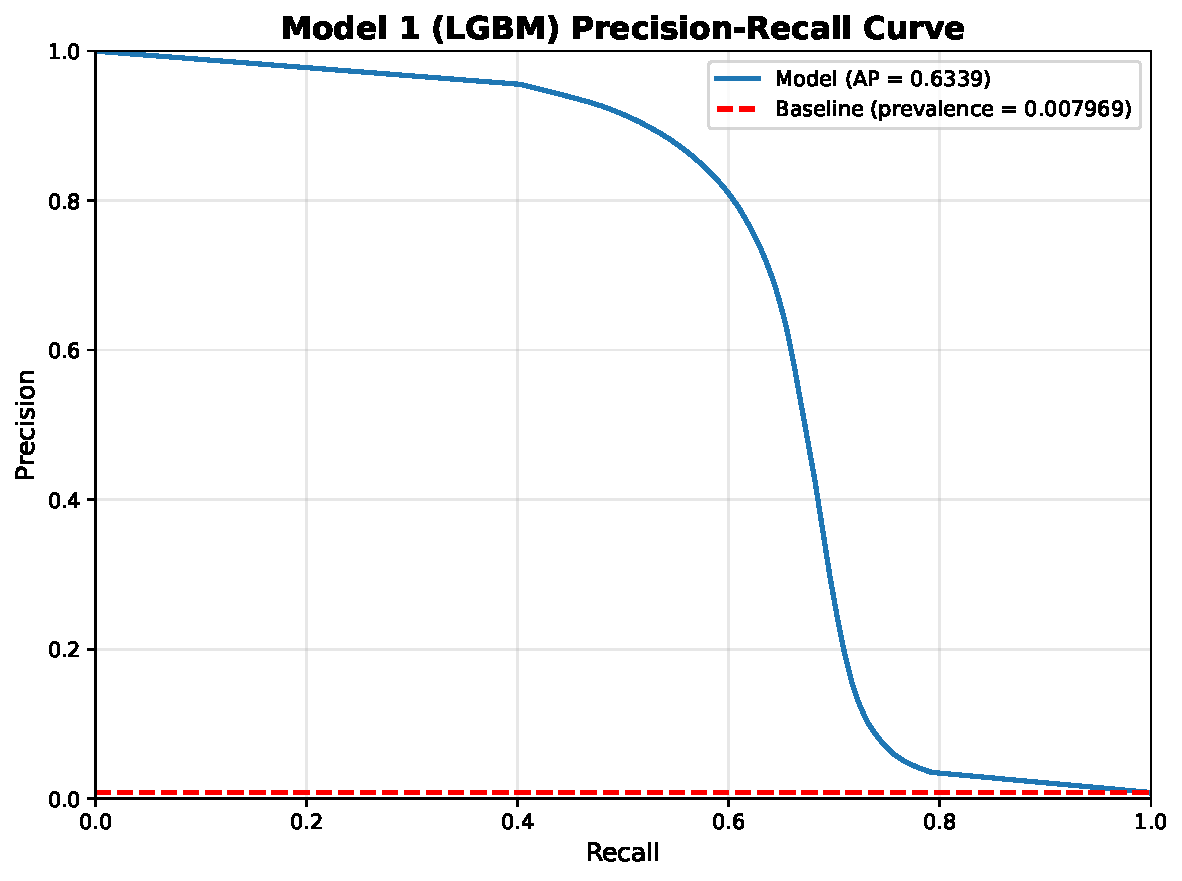
\includegraphics[width=\textwidth, keepaspectratio]{../outputs/south_america/results/model1_lgbm/pr_curve.pdf}
  \caption{Precision--Recall curve. The dashed line shows the random-classifier
  baseline ($\approx 0.8\%$ positive rate). The curve lies far above the baseline
  across the full threshold range.}
  \label{fig:pr_sa}
\end{subfigure}\hfill
\begin{subfigure}[t]{0.48\textwidth}
  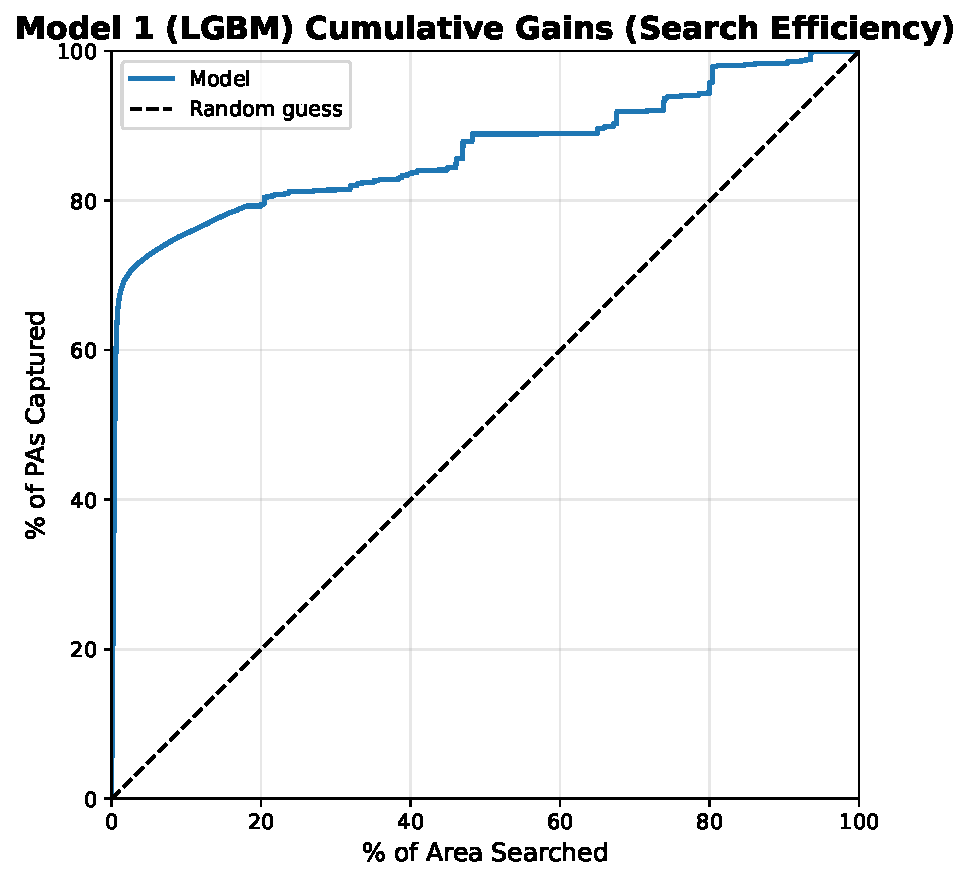
\includegraphics[width=\textwidth, keepaspectratio]{../outputs/south_america/results/model1_lgbm/cumulative_gains.pdf}
  \caption{Cumulative gains chart. The curve shows the fraction of all
  test-period transitions captured as a function of the fraction of pixels
  screened, ranked by predicted probability.}
  \label{fig:cumgains_sa_main}
\end{subfigure}
\caption{Model discrimination for the South America LightGBM on the temporal test set
(2017--2019). \textit{Left:} Precision--Recall curve. \textit{Right:} Cumulative
gains chart --- at the top 1\% of pixels, pixel-year Recall@1\% = 66.8\% and
Lift@1\% = 66.8$\times$; these coincide numerically because Recall@$k$ = Lift@$k \times k$
and $k=0.01$ here.}
\label{fig:pr_gains_sa}
\end{figure}
Figure~\ref{fig:pr_gains_sa} shows the Precision--Recall curve (left panel) and
cumulative gains chart (right panel) for the LightGBM model. As the classification
threshold decreases from right to left, precision (fraction of flagged pixels that
actually transition) falls while recall (fraction of all transitions flagged) rises.
The curve lies far above the dashed baseline throughout, confirming that the
model's advantage over random selection is not an artefact of a single threshold but
holds across the entire operating range. The cumulative gains chart provides a
complementary view from the perspective of recall: at the top 1\% of pixels, the
model captures $\approx$66.8\% of all test-period transitions (Lift $66.8\times$).

Both LightGBM and Random Forest are fully trained and evaluated production models, and
their results confirm each other: the two classifiers produce broadly similar performance
across all metrics. The Random Forest achieves a higher ROC-AUC (0.927 vs.\ 0.897),
while LightGBM leads on PR-AUC (0.645 vs.\ 0.634), Brier score (0.00421 vs.\ 0.00458),
and ECE (0.0081 vs.\ 0.0109). For transition-risk applications, PR-AUC and probability
calibration are the more actionable metrics. LightGBM is therefore reported as the
primary model in the remainder of the analysis, with RF results provided for confirmation.
Substantive conclusions about designation drivers and the 30$\times$30 gap are robust
to this choice; the cross-continental transfer analysis reveals meaningful LGBM/RF
differences (Appendix~\ref{app:transfer}) that are discussed in Section~\ref{sec:disc_transfer}.

\subsubsection{Event-Level Coverage}
\label{sec:results_sa_events}

Pixel--year metrics such as PR-AUC penalise any error in timing: a model that
correctly identifies the \emph{location} of a future designation but places it one
year off still receives no credit for that positive. For a policy application such as
screening land for transition risk, the question of interest is spatial rather than
temporal: does the model identify the right \emph{places}, regardless of precisely
when designation occurs within the next five years?

Event-level coverage answers this question directly: for each unique PA establishment
event within the five-year prediction window, the metric checks whether that event's
location falls within the top-1\% risk zone. The prediction window for each test-year
observation extends five years forward: 2017 test rows look ahead to 2022, 2018 to
2023, and 2019 rows to 2024. This definition is identical to the
\texttt{transition\_01\_win5} label used for all pixel--year metrics, making
event-level recall directly comparable to Recall@K. A ``unique PA establishment event'' is defined as a unique pixel that transitions
for the first time within any test-year's five-year prediction window; pixels that
appear as positives in multiple test years (due to overlapping windows) are counted
only once. The top-1\% risk zone is computed as a fixed threshold on the 2017
test-year scores, and event-level metrics are evaluated against all unique designated
pixels across the 2017--2024 window. Under this aggregation,
the LightGBM model achieves a \textbf{Recall@1\% of 77.4\%} and a
\textbf{Precision@1\% of 79.8\%}: nearly four in five of the top-1\% predicted
pixels actually became protected areas, and three in four of all new protected areas
fell within just 1\% of eligible land (approximately 159,000~km$^2$ out of
15.9~million~km$^2$). In other words, a risk analyst screening fewer than 1\% of
candidate parcels would flag roughly three-quarters of all future designation events
well in advance, while maintaining a precision rate close to 80\%. This combination of high precision \emph{and} high recall at an extremely concentrated
threshold is the defining result: the moderate pixel--year PR-AUC is consistent with
the inherent difficulty of predicting the exact year of a politically-driven
administrative decision, rather than a failure of spatial targeting, though a formal
decomposition of errors into wrong-year/right-place versus wrong-place categories
has not been conducted.

\subsubsection{Probability Calibration}
\label{sec:results_sa_calibration}

Before Platt scaling, raw LightGBM scores are systematically overconfident in the
high-probability range (the reliability diagram in Appendix~\ref{app:calibration}
illustrates the pre-calibration bias). After calibration, the ECE drops to 0.0081.
High-score bins contain few observations due to the rare-event structure; calibration
in the upper tail should be interpreted with reference to the reliability diagrams
rather than aggregate ECE alone.

The practical implication is that a pixel with a calibrated predicted probability of
0.03 has a 3\% chance of being designated within five years, a statement that is
meaningful for portfolio screening and risk quantification, not merely for ranking.

\subsubsection{Feature Importance (SHAP)}
\label{sec:results_sa_shap}

Figure~\ref{fig:shap_sa} shows the SHAP summary plot for the South America LightGBM
model on the test set. Each row is one feature, sorted from top (highest mean absolute
SHAP value) to bottom. For each observation, the horizontal position of a dot shows
that feature's SHAP value, measuring how much it pushed the prediction above (positive) or
below (negative) the mean prediction. Dot colour encodes the raw feature value
(red = high, blue = low). The plot simultaneously conveys both the average importance
of a feature and the direction and nonlinearity of its effect.

\begin{figure}[H]
\centering
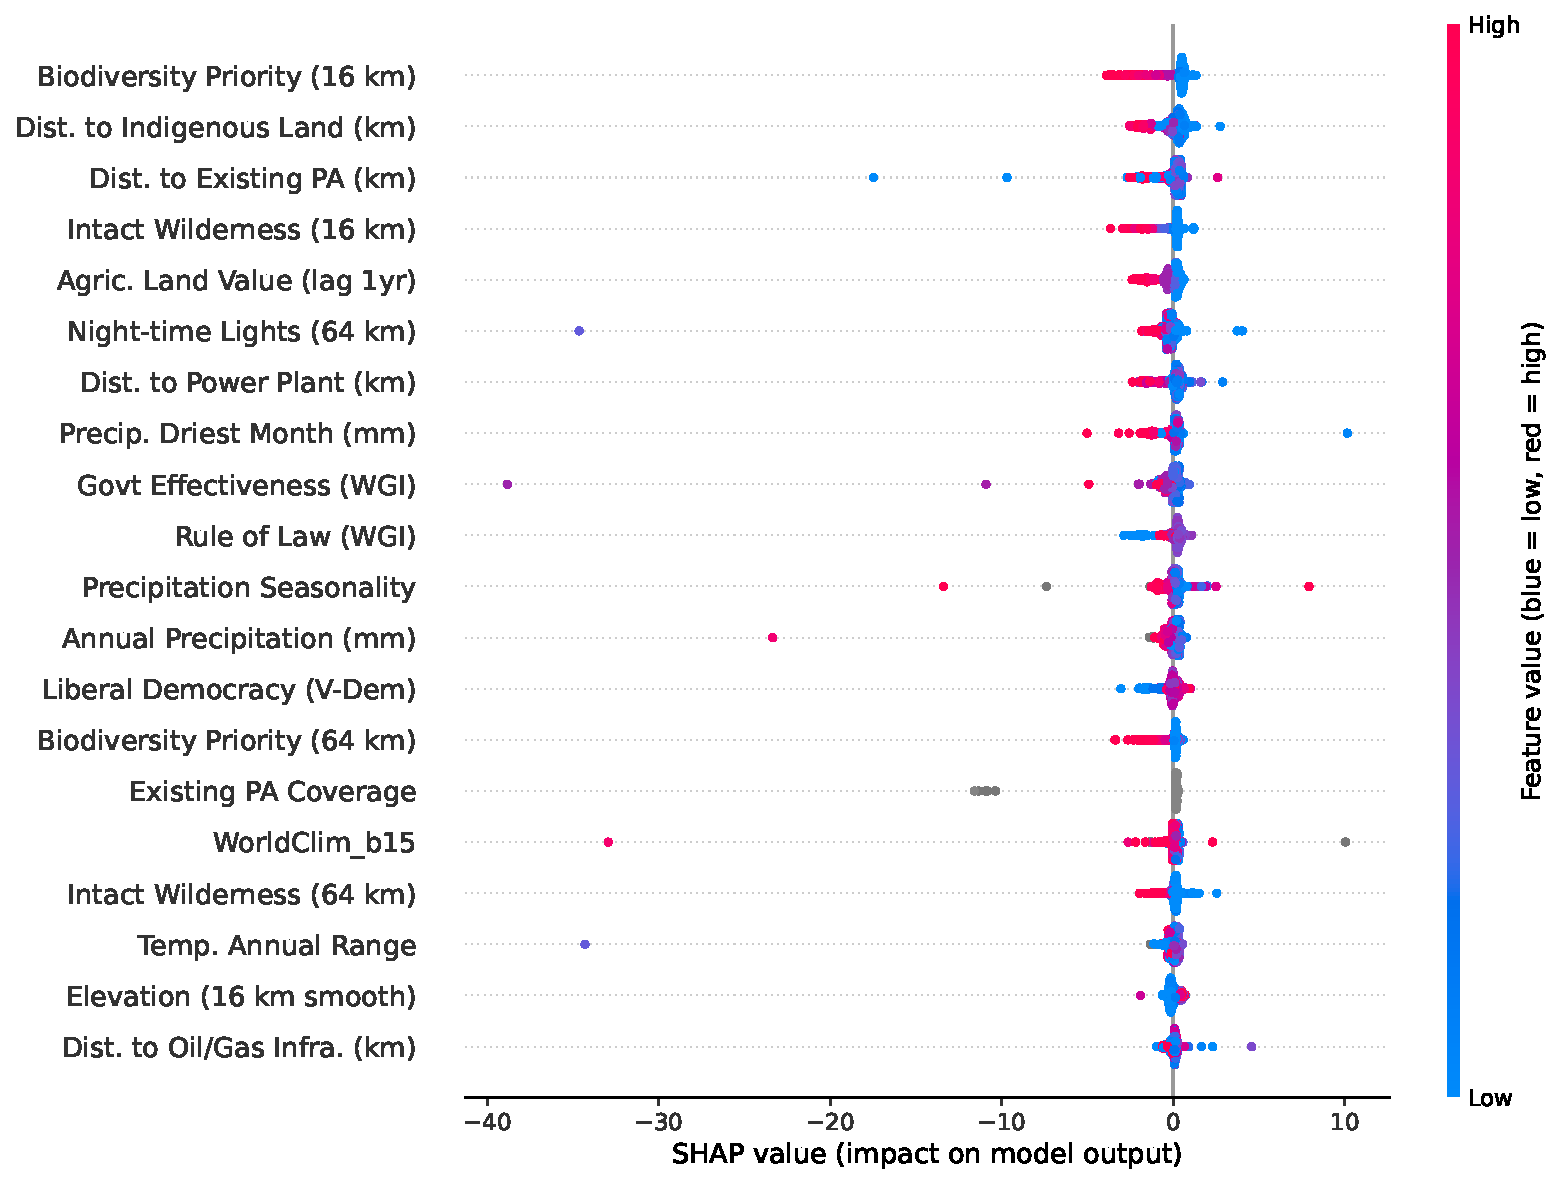
\includegraphics[width=0.60\textwidth, keepaspectratio]{../outputs/south_america/results/model1_lgbm/shap_summary.pdf}
\caption{SHAP summary plot for the South America LightGBM model (test set 2017--2019).
Features are sorted by mean absolute SHAP value (top = most important). Each dot
represents one pixel--year observation; horizontal position is the SHAP value (positive
= increases predicted designation probability; negative = decreases it); the colour bar
on the right indicates the raw feature value (blue = low, red = high). Feature names
have been translated from internal codes to interpretable labels.}
\label{fig:shap_sa}
\end{figure}

The SHAP rankings partly confirm and partly qualify the simple opportunity-cost
narrative. Three co-determining channels emerge:

\textbf{Ecological conservation priority.} The two leading individual features are
High Biodiversity Areas at 16~km and 64~km smoothing
(\texttt{GSN\_b2\_smooth16}, \texttt{GSN\_b2\_smooth64}) and Intact Wilderness
at 16~km (\texttt{GSN\_b3\_smooth16}). Their positive SHAP values indicate that
pixels embedded in globally significant biodiversity and wilderness areas attract
designation, consistent with the ecological-value channel documented in conservation
siting studies \citep{mouillot2024}. The dominance of spatially smoothed versions of these layers over the raw pixel-level
indicators is consistent with designation being a landscape-scale process that responds
to the \emph{ecological neighbourhood}, not just the individual pixel; the pattern may
also partly reflect correlation between raw and smoothed versions that the model resolves
in favour of the smoother.

\textbf{Institutional capacity.} WGI Rule of Law (\texttt{policy\_b4}) is the
second most important individual feature overall, comparable in magnitude to
the top GSN layers, followed by V-Dem Liberal Democracy Index (\texttt{policy\_b2})
and WGI Government Effectiveness (\texttt{policy\_b3}). Their positive SHAP values indicate that designation probability is higher in countries
with stronger institutions, consistent with the view that institutional capacity
enables international conservation commitments to be translated into on-the-ground
designations \citep{watson2014}. Because governance indicators are assigned
uniformly at country level, they partially proxy country-level base rates; the
association therefore captures genuine governance effects alongside base-rate
variation across countries.

\textbf{Economic opportunity cost and path dependence.} Agricultural land value
(\texttt{economic\_\allowbreak{}value\_\allowbreak{}lag1}) is a mid-tier predictor with predominantly negative
SHAP values: high-value agricultural pixels are systematically suppressed from
high-risk zones, consistent with the opportunity-cost mechanism documented in
\citet{joppa2009}. This is a predictive association; causal identification would
require ablation or exogenous variation in agricultural value.
Distance to indigenous territories (\texttt{dist\_indigenous}) has mixed-sign SHAP
values, reflecting the dual role of indigenous lands: they can both attract
neighbouring designations (conservation buffer zones) and absorb designation pressure
directly through community-based protections. Distance to the existing PA network
(\texttt{dist\_wdpa}) contributes positively at intermediate distances, capturing
the incremental expansion of PA buffers. Infrastructure variables (night-time lights,
roads, population density) appear at a lower tier but with consistent negative
SHAP values, confirming that economic activity deters designation.

The overall picture is one of \emph{complementarity}: designation is most likely
where ecological conservation value is high, institutional capacity is present, and
economic opportunity cost is low. These three conditions do not generally co-occur
randomly: remote, biodiverse areas tend to have lower agricultural value, which
is precisely why the literature characterises historical PA siting as biased toward
economically marginal land \citep{joppa2009, venter2018}. The SHAP evidence is consistent with this mechanism while also showing that
institutional quality is an important and distinct predictor. SHAP dependence plots
for the four most important features are provided in Appendix~\ref{app:shap_dep}.

\subsubsection{Spatial Risk Maps}
\label{sec:results_sa_maps}

Aggregate metrics confirm that the model discriminates well on average, but the
primary deliverable is a spatially explicit risk surface. Figure~\ref{fig:riskmap_sa_top1}
maps the top 1\% of predicted pixels across South America, overlaid with observed
PA designations within the five-year prediction window (2017--2024). The observed
category spans the full horizon that the model is trained to predict: all
designations that occurred within five years of any test-period observation year
(2017, 2018, or 2019), covering 2017--2022, 2017--2023, and 2017--2024 respectively.
This means the map's recall is directly comparable to the Recall@1\% metric reported
in the benchmark table; both denominators are identical. Of the total PA establishments
captured, a subset occurred during the immediate test years (2017--2019) and the
remainder in the subsequent window (2020--2024), demonstrating that the model's
risk signal persists beyond the held-out evaluation period.

High-risk pixels form spatially
coherent clusters rather than a diffuse pattern, concentrated in the Amazon basin
periphery, the Cerrado--Amazon transition zone, the Andean foothills, and parts of
Chile's southern regions. At Precision@1\% = 79.8\%, almost every cluster on the
map corresponds to a place where a PA was in fact established; the model is not
simply flagging the most biodiverse or remote areas in general, but identifying the
specific locations where governments subsequently acted. The strong spatial correspondence between predicted high-risk zones and realised
designations confirms that the model produces geographically meaningful risk
concentrations; note that Precision@1\% is a pixel-level metric and does not
directly imply cluster-level hit rates, which would require a separate spatial
cluster evaluation.

\begin{figure}[H]
  \centering
  \begin{subfigure}[t]{0.49\textwidth}
    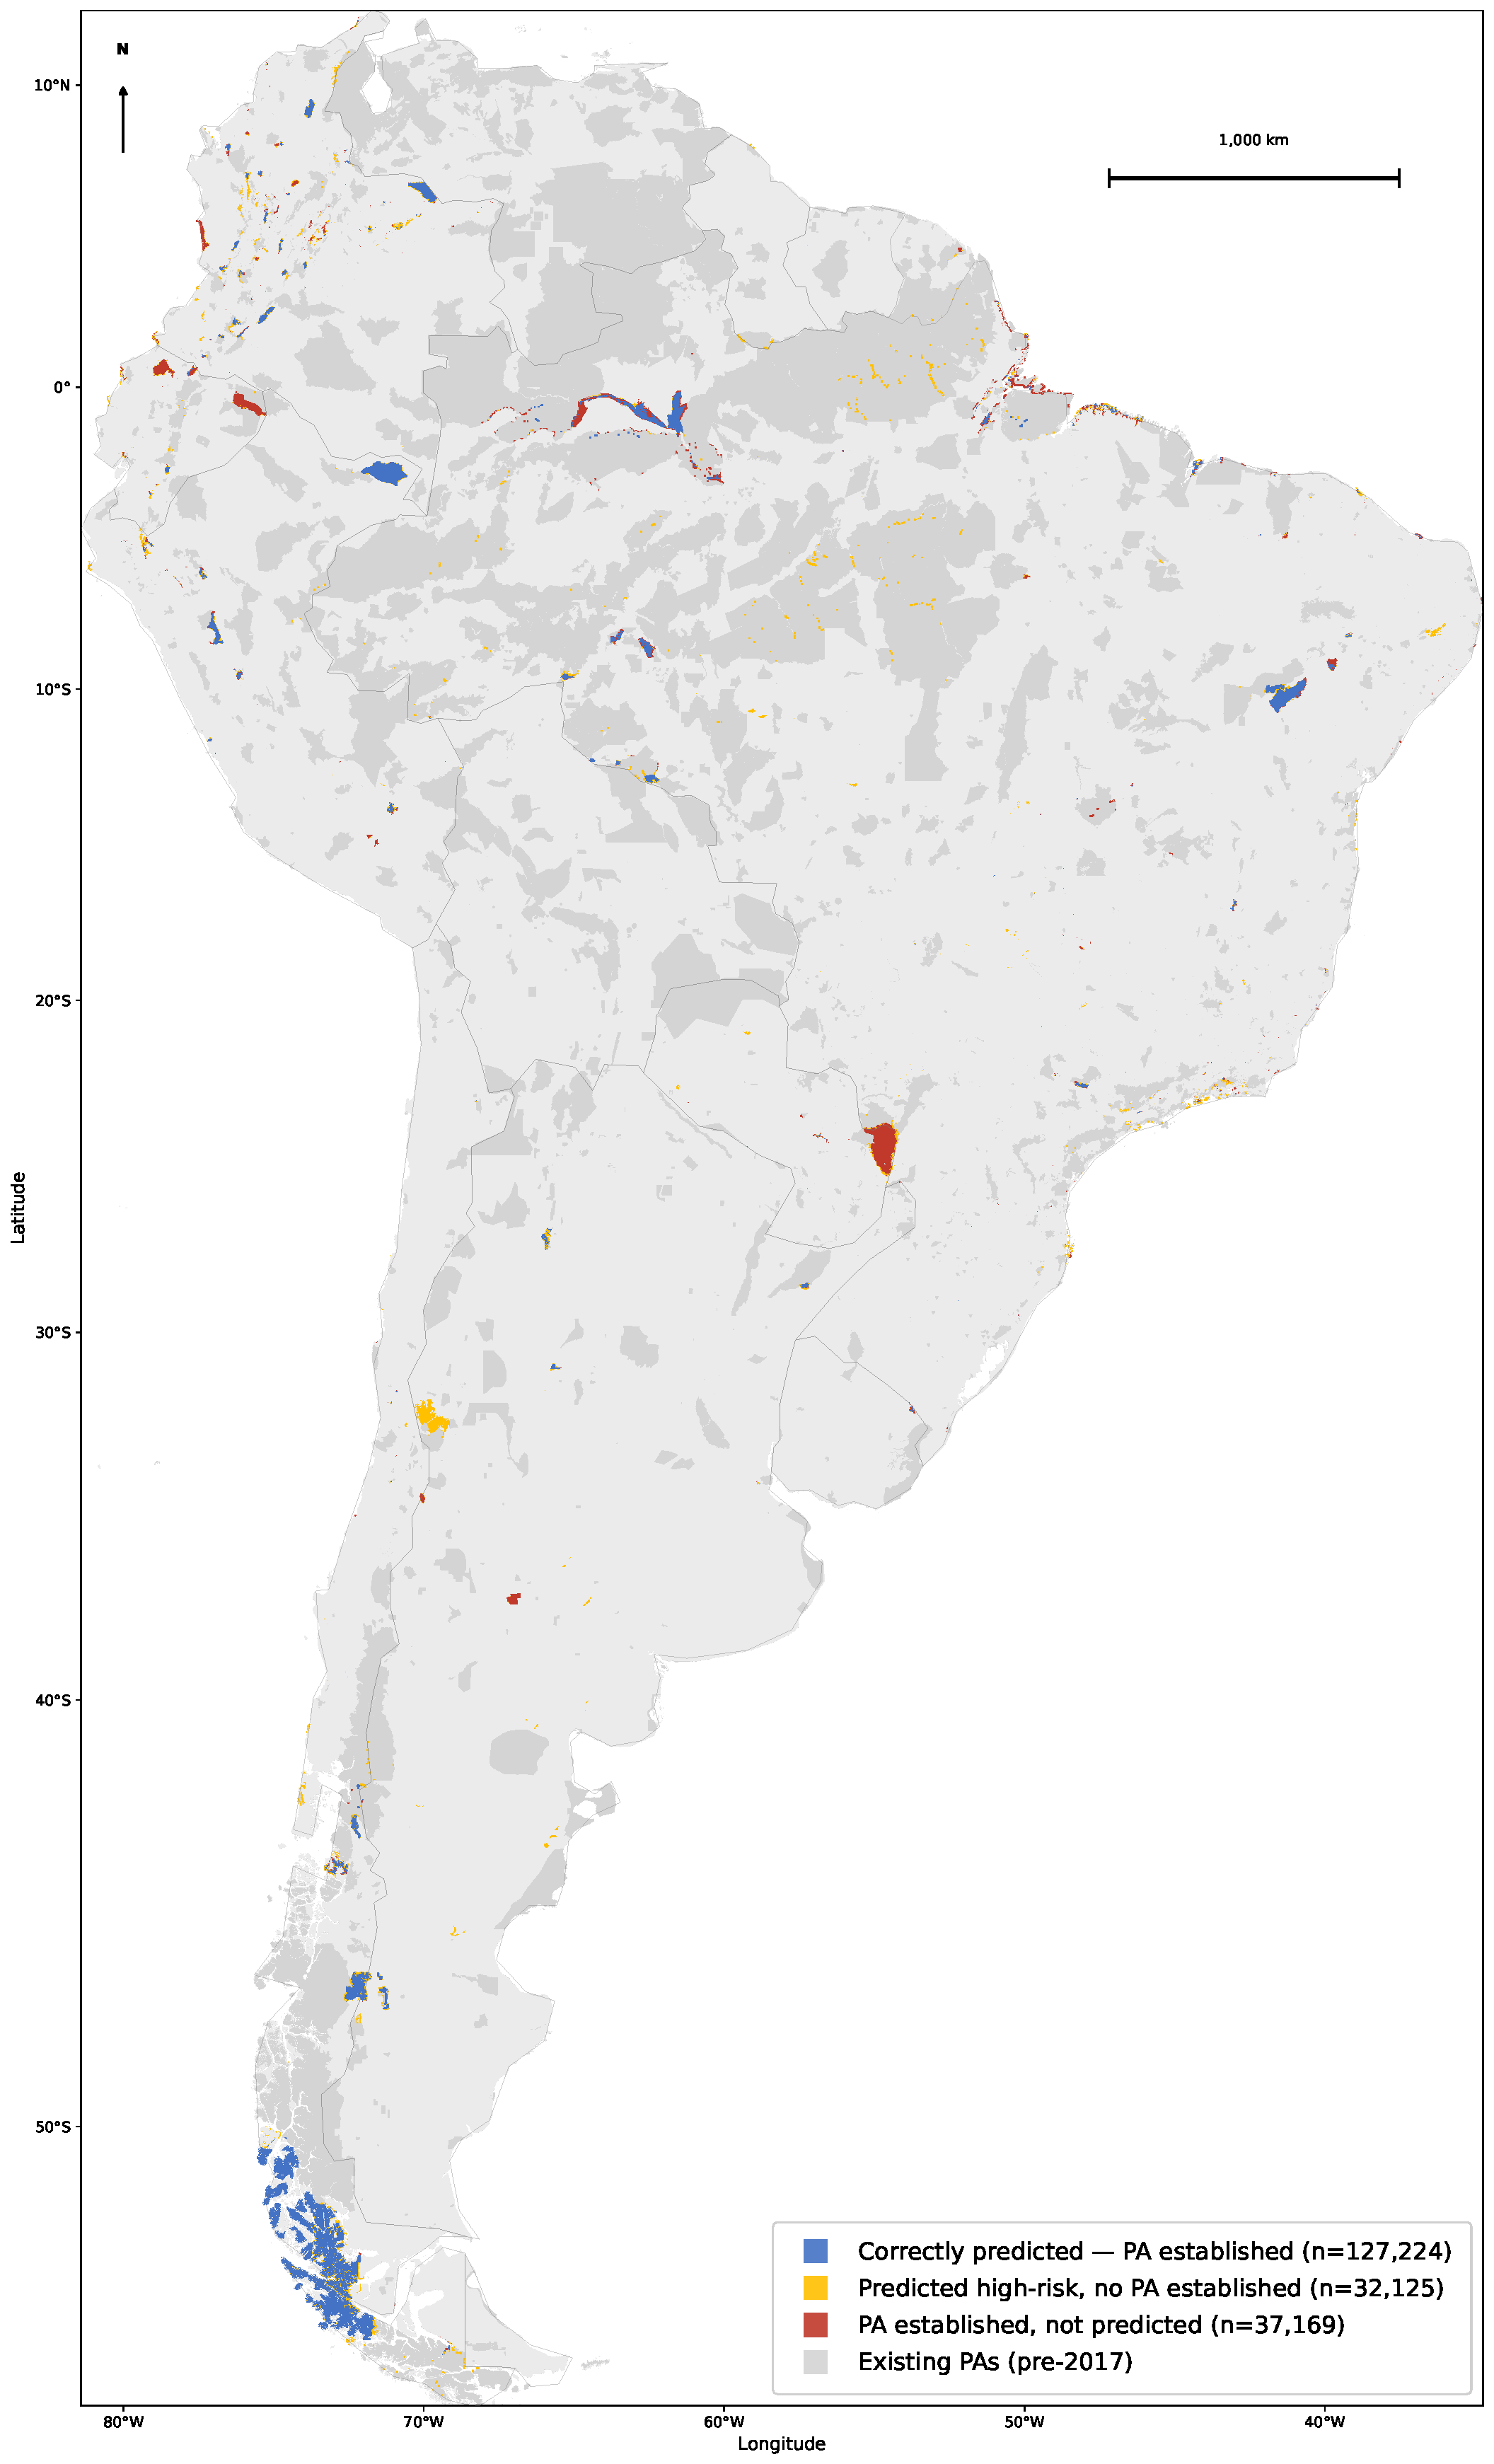
\includegraphics[height=12.7cm, keepaspectratio]{../outputs/south_america/results/model1_lgbm/risk_map_top1pct.pdf}
    \caption{Top 1\% risk map (thresholded)\\
    \textit{\small Blue: true positive; Gold: unconfirmed prediction; Red: model miss; Grey: excluded (already protected)}}
    \label{fig:riskmap_sa_top1}
  \end{subfigure}\hfill
  \begin{subfigure}[t]{0.49\textwidth}
    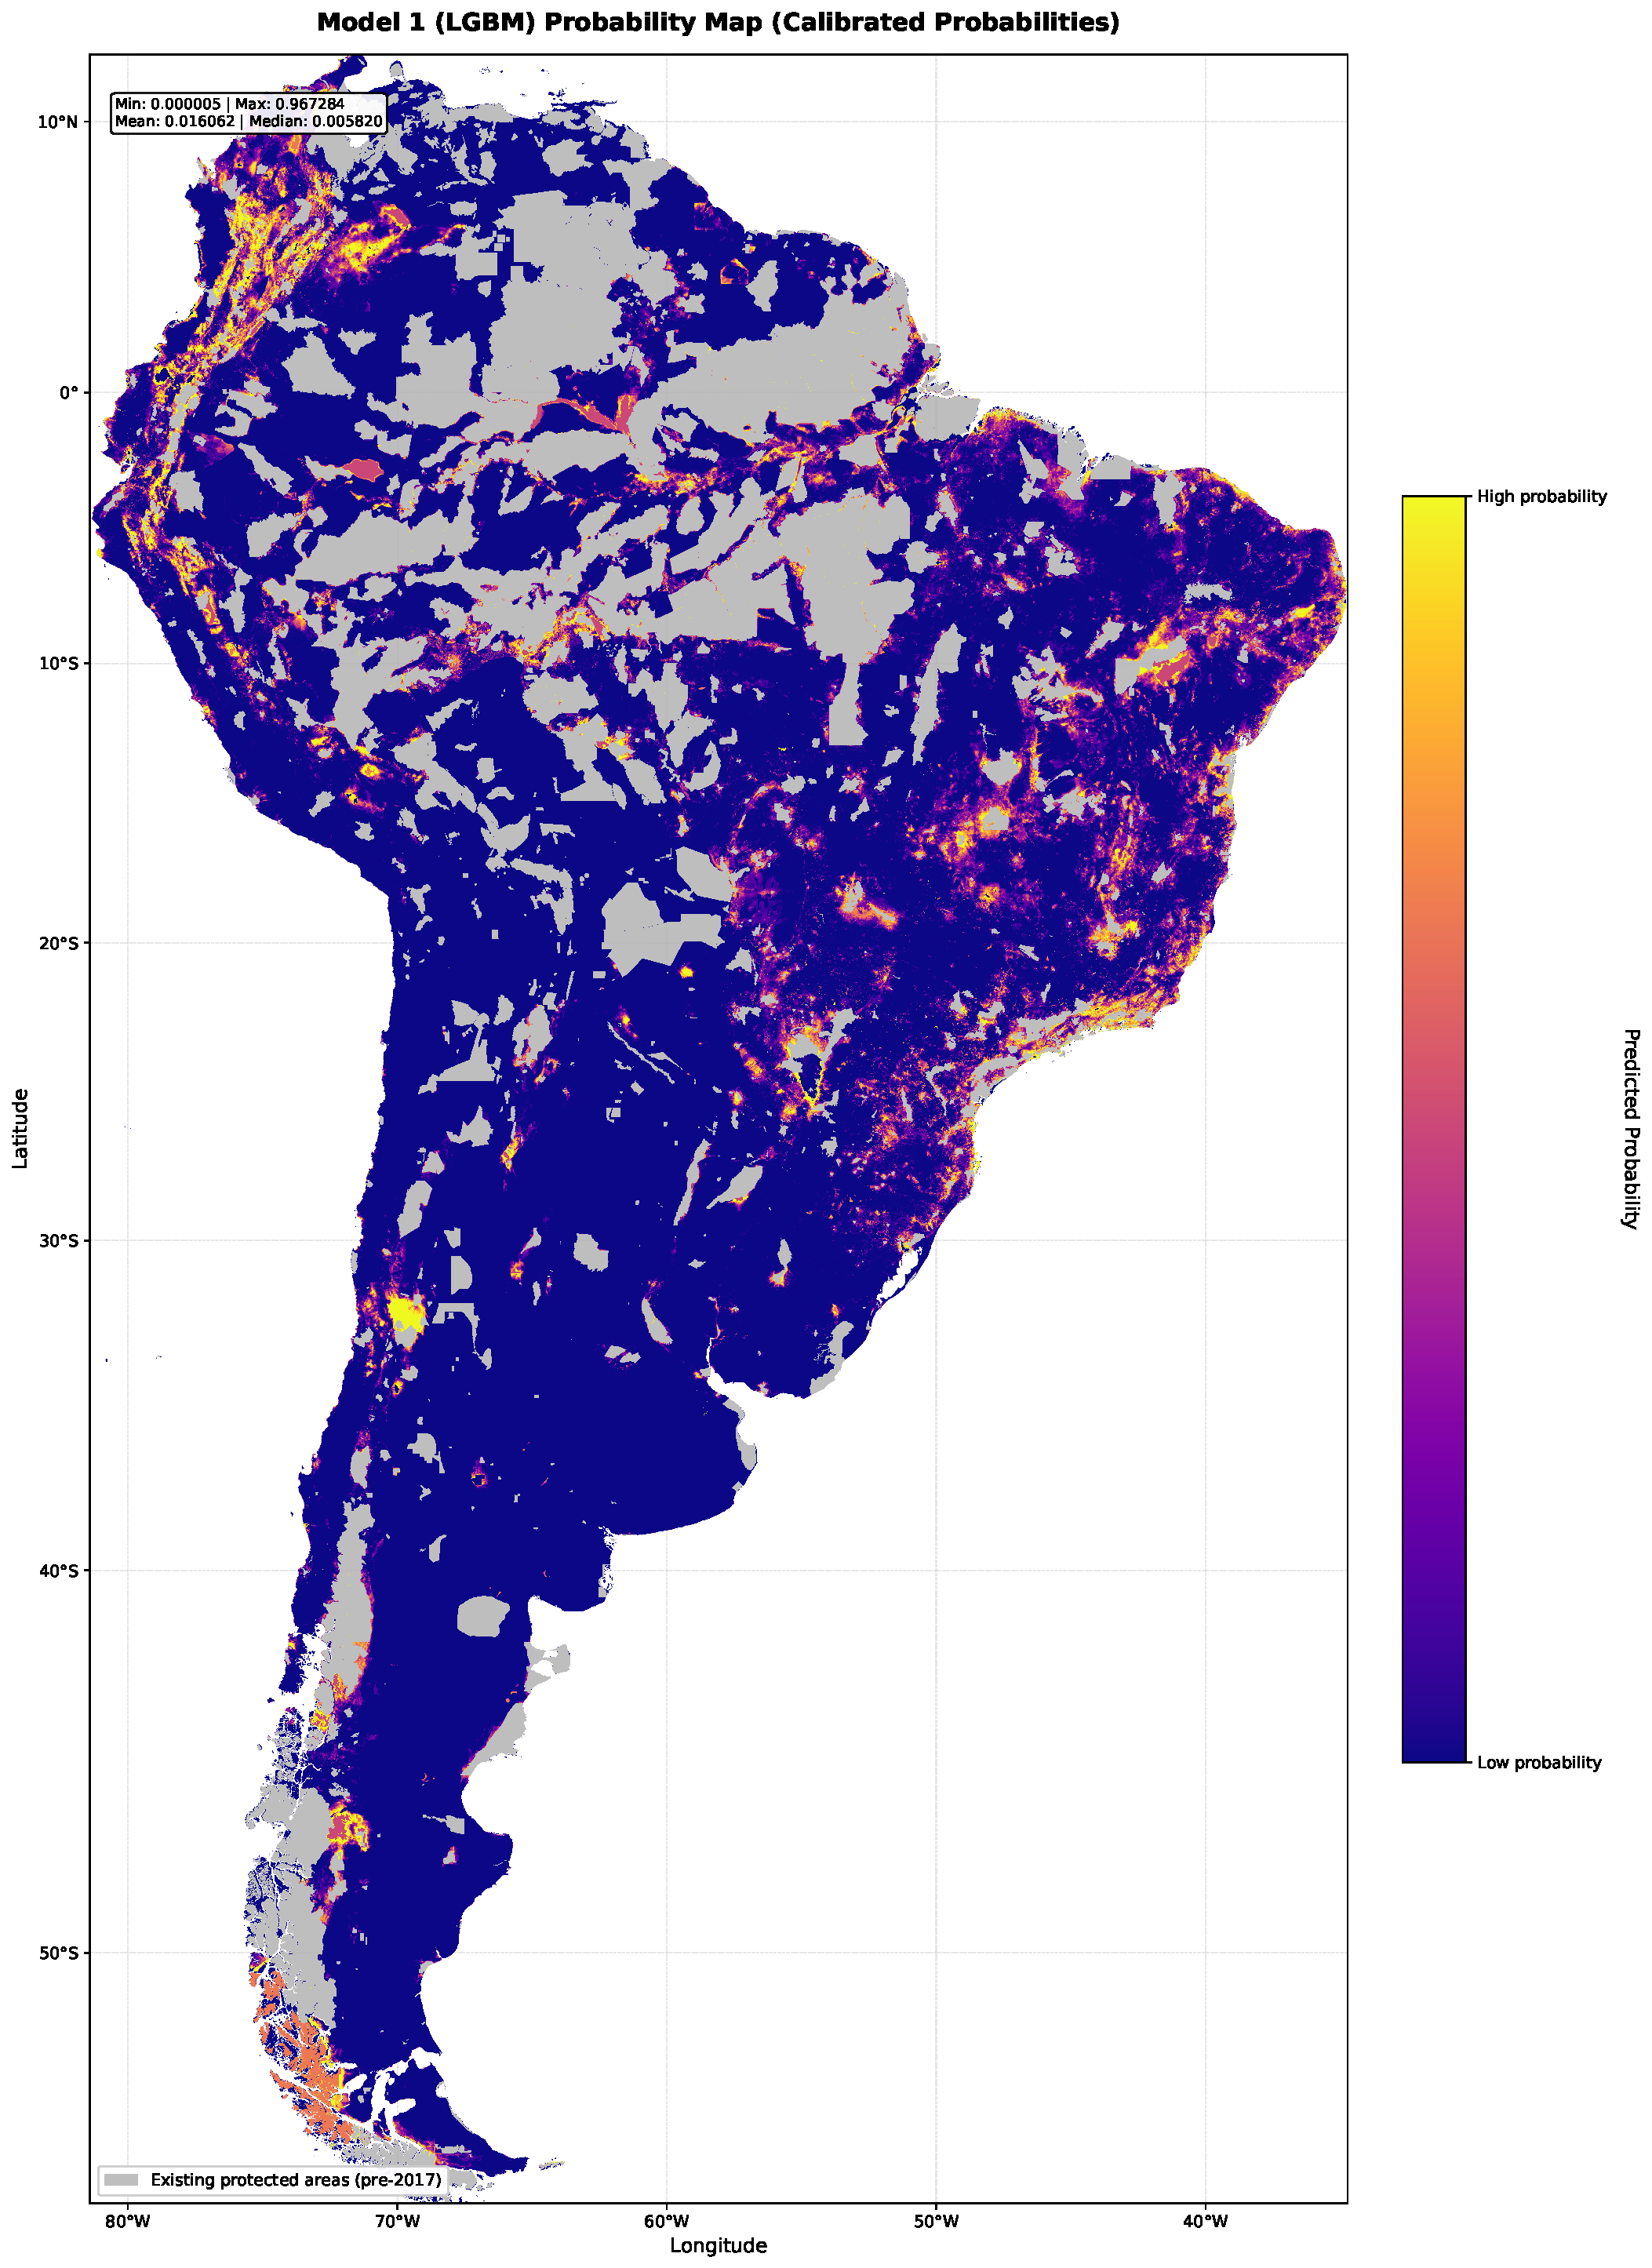
\includegraphics[height=12.7cm, keepaspectratio]{../outputs/south_america/results/model1_lgbm/probability_map.pdf}
    \caption{Continuous calibrated probabilities\\
    \textit{\small Square-root stretch (25th--98th percentile); dark purple = low, yellow = high; grey = excluded (already protected)}}
    \label{fig:probmap_sa}
  \end{subfigure}
  \caption{South America LightGBM transition-risk maps. \textbf{(a)} Top 1\% of predicted pixels (event-level Recall@1\% = 77.4\%, Precision@1\% = 79.8\%; pixel-year Lift@1\% = 66.8$\times$), overlaid with observed PA establishments within the five-year prediction window. \textbf{(b)} Continuous calibrated five-year cumulative designation probabilities, showing a strongly right-skewed distribution with a small upper tail concentrating substantially elevated risk. Probabilities reflect covariate values at the end of the test period.}
  \label{fig:sa_riskmaps}
\end{figure}

% ---------------------------------------------------------------------------
\subsection{Spatial Generalisation}
\label{sec:results_spatial}

Three complementary tests assess how well learned patterns extend beyond the training geography, from biome-level holdouts to cross-continental transfer.

\subsubsection{Leave-One-Biome-Out (LOBO)}
\label{sec:results_lobo}

The LOBO evaluation asks whether the patterns learned on other biomes generalise to
a held-out one (see Section~\ref{sec:lobo} for the methodological rationale).
The LOBO PR-AUC across South American biomes shows substantial variation: the
\textbf{median} across 10 evaluated biomes is \textbf{0.096} (IQR 0.013--0.224);
the mean of 0.233 is dominated by two high-performing temperate biomes (Temperate
Broadleaf 0.904, Temperate Grasslands 0.738) and should not be read as reflecting
average spatial robustness. Expressed as PR-AUC lift (PR-AUC divided by the biome's
positive rate), 9 of the 10 evaluated biomes achieve lift above the random baseline of~1.

Performance varies markedly across biomes.
Temperate Broadleaf and Mixed Forests (Patagonian Chile) achieves the highest
raw LOBO PR-AUC (0.904), consistent with the hypothesis that its distinctive
covariate profile (high elevation, low population density, remoteness) is readily
learnable from other biomes. Temperate Grasslands, Savannas and Shrublands yields
the highest PR-AUC lift (843$\times$), largely because its near-zero positive rate
(0.09\%) amplifies the lift ratio; absolute performance is also strong
(PR-AUC 0.738). These interpretations are descriptive hypotheses, not validated
by biome-level SHAP analysis.

By contrast, Flooded Grasslands and Savannas (Amazonian v\'{a}rzea and Pantanal)
achieves a LOBO PR-AUC lift of 0.6$\times$---the only below-random biome---with
ROC-AUC 0.19. Designation patterns here are not recoverable from the static
continental feature set; plausible explanations include seasonal flood dynamics and
site-specific institutional processes not captured by the available covariates.
Tropical \& Subtropical Grasslands (Cerrado and Llanos) is also near-random
(ROC-AUC 0.48, lift 1.1$\times$) despite forming the largest test fold by area.


\begin{figure}[H]
\centering
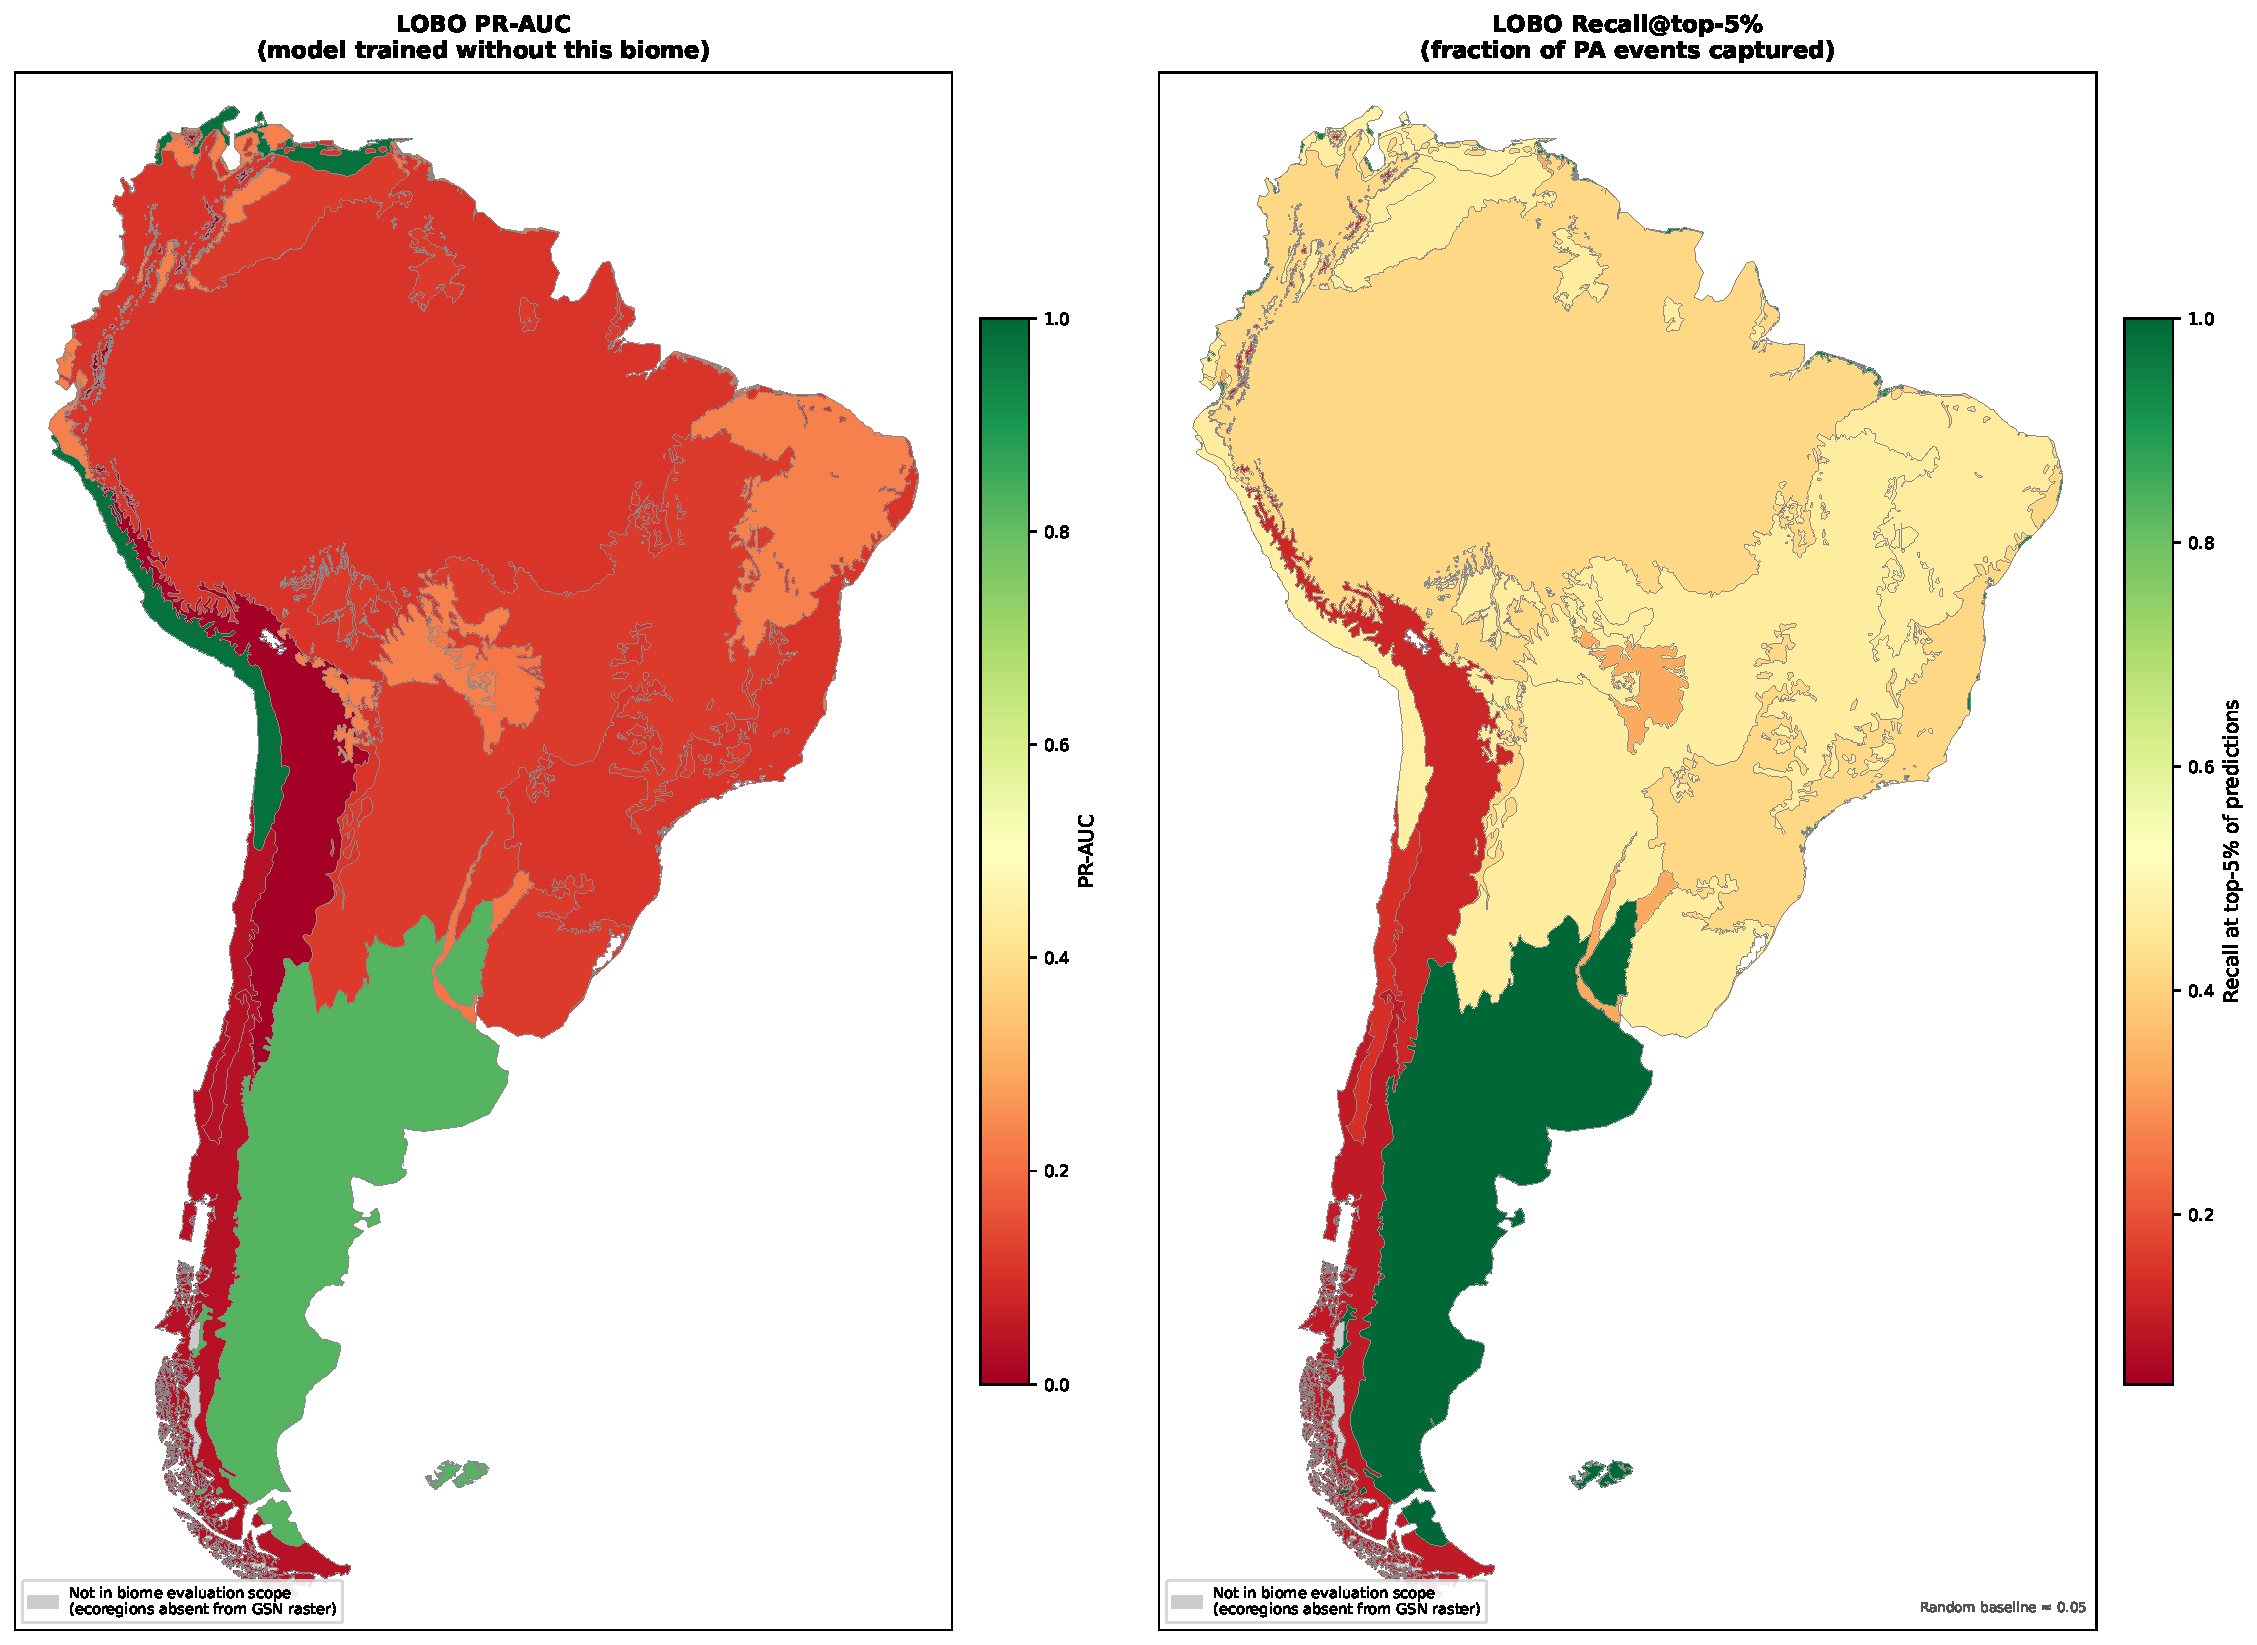
\includegraphics[width=\textwidth, keepaspectratio]{../outputs/south_america/results/spatial_cv_visualisation/map_lobo_performance_lgbm.pdf}
\caption{Geographic distribution of LOBO out-of-sample performance across South American
biomes (LightGBM, test set 2017--2019). Each biome is coloured by its performance when
the model was trained on all \emph{other} biomes (leave-one-biome-out); numbered circles
identify biomes in the key below the map. Grey areas are outside the biome evaluation
scope of the GSN raster.
\textbf{(a) PR-AUC lift} relative to the biome-specific random baseline (PR-AUC divided
by the biome's positive rate); lift $= 1$ is the random classifier; colour scale capped
at 30$\times$ for readability.
\textbf{(b) Recall at the top-5\%} of predicted pixels (absolute fraction), anchored at
5\% (the universal random baseline); colour scale capped at 70\% to spread contrast
across the informative range. This panel answers directly the policy question: ``If a
decision-maker screens the top-5\% of land flagged by the model, what share of all
future protected-area designations in that biome would be captured?'' Green biomes
(Temperate Broadleaf \& Mixed Forests, Deserts \& Xeric Shrublands) exhibit spatial
patterns recoverable from continental gradients alone; red and yellow biomes
(Flooded Grasslands \& Savannas, Tropical Moist Broadleaf Forests) are governed by
localised institutional and dynamic processes not captured by the static feature set.}
\label{fig:lobo_sa_map}
\end{figure}

% ---------------------------------------------------------------------------
\subsubsection{Cross-Regional Transfer}
\label{sec:results_cv3}

To test whether learned patterns are universal or continent-specific, the production
models are applied across all three continental pairs without retraining, using the
common 73-feature set. The SA\textendash{}USA corridor provides the cleanest test: the SA
LightGBM model applied to the US test set achieves ROC-AUC $= 0.517$; the US model
applied to the SA test set achieves ROC-AUC $= 0.518$, both indistinguishable from a
random classifier. PR-AUC is below 0.01 in both directions.

Extending the evaluation to Southeast Asia reveals a more heterogeneous but consistent
pattern of transfer failure. LGBM transfers from the SE Asia model into the Americas
are severely below random: SE Asia $\to$ South America ROC-AUC $= 0.381$; SE Asia
$\to$ USA ROC-AUC $= 0.238$. The reverse directions are near-random (SA $\to$ SE
Asia: 0.521) or moderately above (USA $\to$ SE Asia: 0.617). Below-random performance
indicates that the features most predictive of designation in SE Asia are
\emph{anti-correlated} with designation in the Americas: what the SE Asia model
ranks as high-risk is systematically low-risk in the other regions. Full results
across all twelve directions (LightGBM and Random Forest cross-regional transfer for all three regions) are in
Appendix~\ref{app:transfer}.

This transfer failure is itself a substantive result. The near-random or below-random
LGBM cross-transfer is consistent with \emph{institutional specificity} of PA
designation patterns, but several technical explanations cannot be ruled out: the
common feature set uses numeric codes for categorical variables (ecoregion, land
cover) that carry different ordinal relationships across regions; base rates differ
by an order of magnitude across regions, causing calibration mismatch; and gradient-boosted
models may overfit to region-specific correlational patterns. These alternatives are
partially addressed by the RF transfer results, which show substantial transfer in
several directions (Appendix~\ref{app:transfer}), suggesting that gradient-boosting
overfits more strongly to regional idiosyncrasies than the bagged RF ensemble.

For LightGBM, each regional model has learned the specific feature-to-designation
mapping in its own governance context and does not transport to others; for Random
Forest, partial transfer is observed in several directions (SA$\to$SEA: 0.720;
SEA$\to$USA: 0.713), suggesting that the RF's bagged architecture captures more
transferable ecological baselines while LGBM overfits to region-specific institutional
patterns. The practical implication is that LGBM-based transition-risk scores
require region-specific models; whether RF-based scores could support global
risk assessment with a shared feature set requires further investigation.

% ---------------------------------------------------------------------------
\subsubsection{Biome-Stratified Performance}
\label{sec:results_biome_strat}

The biome-stratified evaluation uses the full production model to examine where within
each continent risk scores are most and least actionable. Unlike LOBO, which withholds
biomes from training, this diagnostic reveals where prediction is harder even with
the biome's own history available.

Figure~\ref{fig:biome_breakdown_sa} shows per-biome ROC-AUC and Lift@1\% for South
America. ROC-AUC is high across all biomes ($\geq$0.62; seven of nine exceed 0.81).
Lift@1\% reveals sharper variation: Temperate Broadleaf \& Mixed Forests achieves
both the highest ROC-AUC (0.97) and high absolute Lift (22$\times$). Flooded
Grasslands \& Savannas achieves high ROC-AUC (0.98) but moderate Lift (97$\times$
at face value) masking near-zero absolute precision, because its positive rate is
only $\approx$0.03\%---even highly ranked pixels rarely transition.

The Flooded Grasslands comparison with the LOBO result is instructive: it is the
only biome with below-random LOBO lift yet high within-sample ROC-AUC. Together,
the two results indicate that designation follows a coherent but idiosyncratic
pattern not shared with neighbouring biomes---learnable from its own history, but
not transferable from others.

\begin{figure}[H]
\centering
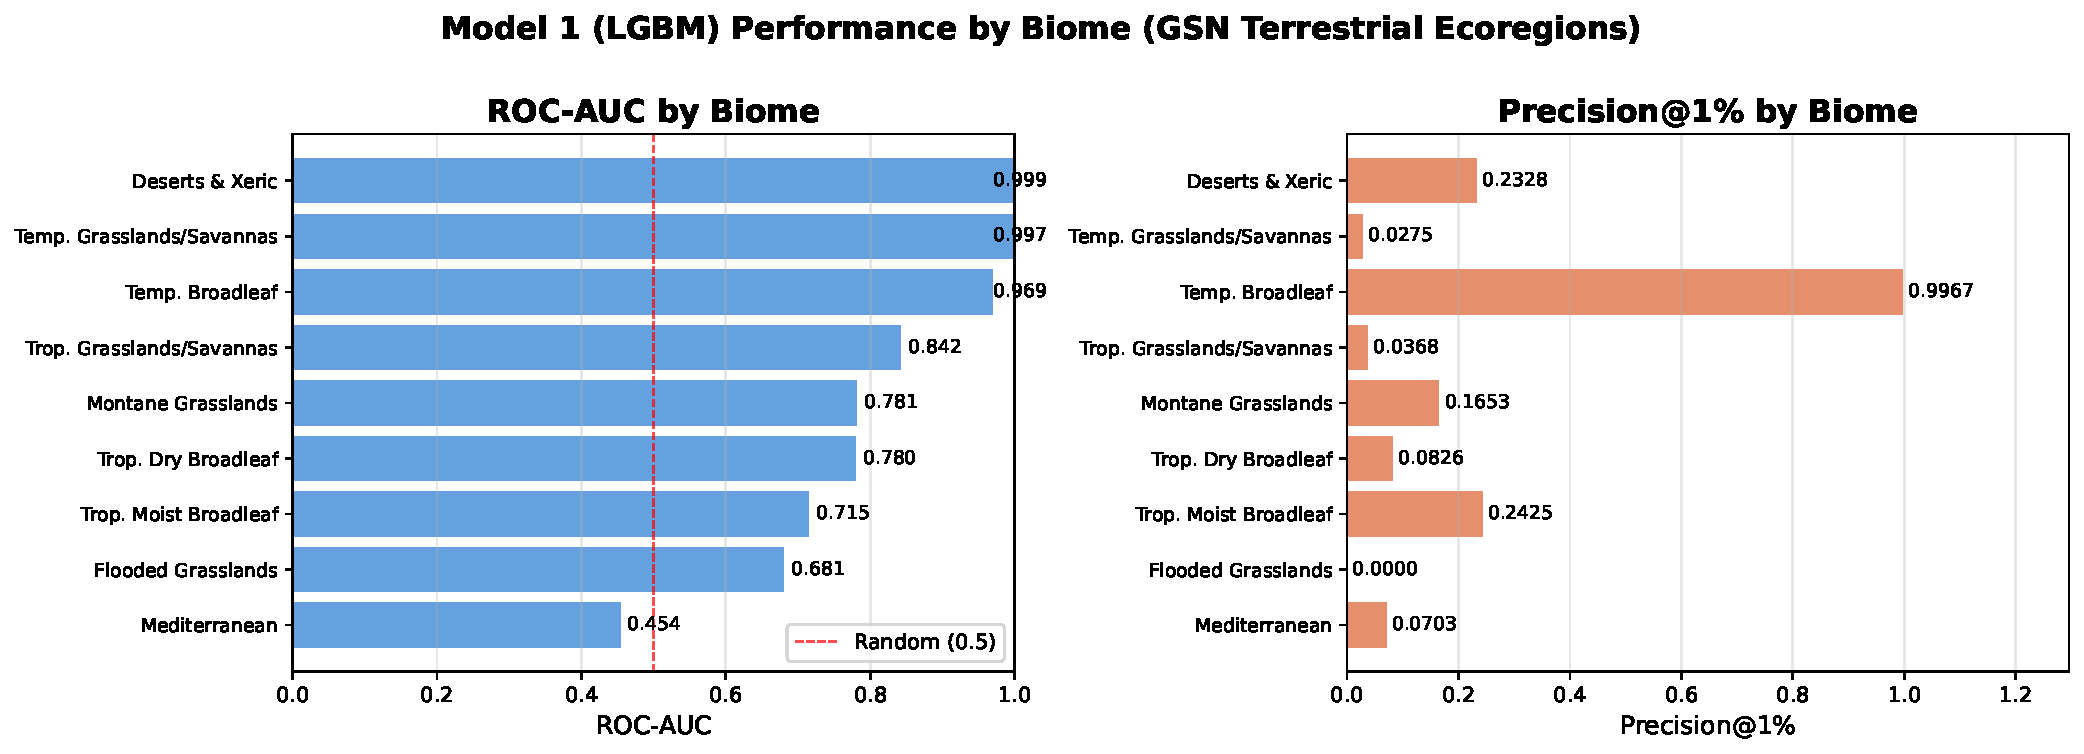
\includegraphics[width=\textwidth, keepaspectratio]{../outputs/south_america/results/model1_lgbm/biome_breakdown.pdf}
\caption{South America biome-stratified performance (full production LightGBM model,
test set 2017--2019). Left: ROC-AUC by biome. Right: Lift@1\% (Precision@1\% divided
by biome positive rate), the random baseline being 1$\times$.
High ROC-AUC coexists with moderate Lift@1\% in low-prevalence biomes (Flooded
Grasslands, Temperate Grasslands, Deserts) because absolute precision remains low
even when relative enrichment is substantial.}
\label{fig:biome_breakdown_sa}
\end{figure}

Biome-stratified breakdowns for the United States and Southeast Asia are in
Appendix~\ref{app:supp_figures} (Figures~\ref{fig:biome_breakdown_usa}
and~\ref{fig:biome_breakdown_seasia}). US ROC-AUC is uniformly high (0.93--0.995),
but Lift@1\% is near-random across all biomes due to the near-zero national positive
rate ($\approx$0.04\%). In Southeast Asia, Tropical Dry Broadleaf Forests and
Temperate Conifer Forests achieve high Lift@1\%, reflecting higher positive rates
(1.07\% and 25\% respectively).

% ---------------------------------------------------------------------------
\subsection{Regional Results}
\label{sec:results_regional}

Results for the United States and Southeast Asia replicate the South America framework across structurally distinct institutional contexts; the section closes with a cross-model comparison.

\subsubsection{United States}
\label{sec:results_usa}

The US results confirm that the predictive framework extends to a structurally
different institutional context. The overall LightGBM ROC-AUC on the US test set is
0.947, indicating strong overall rank discrimination. However, the PR-AUC is only
0.093, reflecting the extreme class imbalance in the US test set ($\approx 0.04\%$
positive rate, 20 times rarer than South America). The high ROC-AUC alongside the
very low PR-AUC reflects the known divergence of these two metrics under extreme
imbalance \citep{davis2006}: the model ranks positives above negatives in aggregate
but struggles to maintain high precision at any fixed threshold. The Lift at top 1\%
is 81.3$\times$, confirming that the top-ranked pixels are genuinely enriched
for future designations even when the absolute precision is low. A consequence of
this lift is that screening only the top-1\% highest-risk pixels captures approximately
81.4\% of all test-period US designations (recall at 1\%), the relevant figure for a
risk officer asking ``what fraction of future PA events would I have flagged?'' rather
than ``how many of my flagged pixels actually transitioned?''
The Random Forest achieves a marginally higher ROC-AUC than LightGBM in the US
setting, confirming that the RF is a competitive alternative and that results are
not sensitive to model choice.

With an absolute Precision@1\% of only 3.3\%, the US model's practical utility for
parcel-level decisions is limited: a risk analyst screening the top-1\% of pixels
would encounter roughly 97 false positives per true positive. For portfolio-level
screening at larger spatial aggregation (county, watershed, lending portfolio), the
high Lift@1\% ($81\times$) means the model substantially outperforms random
selection in identifying regions with elevated PA risk, even if individual pixel
precision is low.

A striking feature of the US data is the geographic concentration of designations:
approximately 85\% of all test-period PA establishments fall within the Deserts and
Xeric Shrublands biome (Bureau of Land Management public land in the American West).
This concentration simplifies the prediction problem in one sense, since any model that
learns to prioritise arid BLM land will score well overall, while creating severe
imbalance for all other biomes.

The LOBO analysis reveals near-zero generalisation across US biomes, with a mean
LOBO PR-AUC of approximately 0.001 across 5 evaluable biomes (Table~\ref{tab:lobo_usa}).
All biome folds achieve PR-AUC lift near or below 1, confirming
that the model's discrimination is highly biome-specific and does not transfer
across ecological contexts. Consistent with the federal land tenure hypothesis,
approximately 85\% of test-period US designations fall within the Deserts \& Xeric
Shrublands biome, dominated by Bureau of Land Management public land; a model
without parcel-level ownership data cannot learn this signal in a transferable way.
%TODO: NEEDS COMPUTATION: add descriptive statistics showing that positives are geographically concentrated on BLM/federal land (e.g.\ share of test positives on public land) before final submission.

Per-biome LOBO results are tabulated in Table~\ref{tab:lobo_usa} (Appendix~\ref{app:lobo}).
%TODO: NEEDS COMPUTATION: restore fig:lobo_usa from comment environment in appendix, or keep table-only reference.
The spatial distribution of predicted probabilities across the US is shown in
Figure~\ref{fig:probmap_usa} (Appendix~\ref{app:supp_figures}).
Full metrics tables for the US are provided in Appendix~\ref{app:lobo}.

% ---------------------------------------------------------------------------
\subsubsection{Southeast Asia}
\label{sec:results_seasia}

The Southeast Asia model achieves a ROC-AUC of 0.994 on the test set, with a PR-AUC
of 0.919. These high values reflect the geographic concentration of PA designation in the region:
new PAs are predominantly located in forested upland areas of Borneo, Sumatra,
peninsular Malaysia, and the Philippines, which differ sharply from surrounding
lowland agricultural zones. The near-perfect ROC-AUC ($= 0.994$) and high PR-AUC
($= 0.919$) warrant leakage scrutiny: these metrics are unusually high for a
rare-event transition forecast. Checks confirm that no 2024 PA outcomes leak into
the feature vector (all covariates are lagged one year); however, the extreme spatial
segregation of high-risk uplands from low-risk lowlands means a simple
elevation/canopy threshold performs nearly as well as the full model. Additionally,
a small number of large PA polygons in Borneo (Sabah/Sarawak state PAs, Brunei
Heart of Borneo) may drive a disproportionate share of the positive observations; the
Lift@1\% of 94.2$\times$ confirms genuine pixel-level enrichment above and beyond
the macro upland/lowland split. The biome-stratified LOBO metrics
(Appendix~\ref{app:lobo}) provide further evidence of spatially heterogeneous
generalisation across Southeast Asian biomes.

The LOBO analysis for Southeast Asia yields a mean PR-AUC of 0.270 across 5
evaluable biomes (Table~\ref{tab:lobo_seasia}, Appendix~\ref{app:lobo}), with strong
heterogeneity; positive rates for individual biomes are pending confirmation from
corrected Euler outputs (lift values in Table~\ref{tab:lobo_seasia} are marked
as requiring recomputation). Figure-level LOBO visualisation for SE Asia is deferred
pending those outputs.
Despite these limitations, the biome-level PR-AUC pattern in Table~\ref{tab:lobo_seasia}
is interpretable. Temperate Conifer Forests and Tropical Coniferous Forests
generalise well: these biomes have distinctive high-elevation, high-canopy
signatures that transfer across training contexts, producing strong PR-AUC lift.
By contrast, Mangroves, Tropical Dry Broadleaf Forests, and Tropical Moist
Broadleaf Forests show near-random LOBO lift, indicating that designation patterns
in these biomes are driven by highly localised institutional or geopolitical
factors not captured by continental-scale features.
Several biome folds contain too few
positive test observations to support meaningful evaluation and are excluded from the
mean; they do not imply poor performance, only insufficient transition events in
those land types.
%TODO: NEEDS COMPUTATION: positive rates and lift for
% Table~\ref{tab:lobo_seasia} are pending regeneration from corrected Euler
% outputs; restore the bar chart figure once available.

The spatial distribution of predicted probabilities is shown in
Figure~\ref{fig:probmap_seasia} (Appendix~\ref{app:supp_figures}).
Full metrics tables for Southeast Asia are provided in Appendix~\ref{app:lobo}.

% ---------------------------------------------------------------------------
\subsubsection{Cross-Model Comparison}
\label{sec:results_model_comparison}

Figure~\ref{fig:model_comparison_landscape} situates all six trained models (three
regions $\times$ two algorithms) in a unified diagnostic framework. Panel~(a) shows
how targeting precision degrades as the risk zone widens from the top-1\% to the
top-10\% of pixels. Panel~(b) relates global discrimination (ROC-AUC) to practical
targeting effectiveness (Lift@1\%), placing both algorithms for each region in the
same space.

Two findings stand out. First, Southeast Asia and South America share nearly identical
\emph{absolute} precision profiles despite very different ROC-AUC values: at the
top-1\% threshold, both the South American ($P{=}0.53$) and Southeast Asian
($P{=}0.56$) LightGBM models flag pixels that subsequently became protected areas
with roughly equal accuracy. The United States, by contrast, achieves dramatically
lower absolute precision ($P{=}0.033$ at top-1\%), not because discrimination is
weak---ROC-AUC exceeds 0.94---but because designation events are so rare
(baseline rate $\approx 0.04\%$) that even a highly ranked pixel is unlikely to
transition. This exposes an important distinction: Lift measures how many times
\emph{better than random} the model performs, while Precision measures the absolute
hit rate a policy-maker would observe in the field. Both are high in Southeast Asia
(Lift $94\times$, $P{=}0.56$), but the US achieves extreme Lift ($81\times$, RF:
$100\times$) against a near-zero baseline.

Second, Random Forest and LightGBM occupy distinct positions within each region
(panel~b). In the United States the RF achieves near-perfect ROC-AUC (0.999) and
Lift@1\% of $100\times$. This near-perfect score warrants caution: it likely
reflects the extreme geographic concentration of US designations in a single BLM
biome that is easy to rank-separate from the rest, potentially amplified by a
dominant spatial proxy variable (distance to existing PA network or federal land
boundary). Temporal leakage has been ruled out, but the result should be interpreted
as upper-bounding performance in this specific geographically concentrated context
rather than as a general benchmark achievement. In South America the two algorithms
converge, with RF slightly improving ROC-AUC (0.927 vs.\ 0.897) at marginal cost
to calibration. These within-region differences are documented in
Appendix~\ref{app:lobo}.

\begin{figure}[H]
\centering
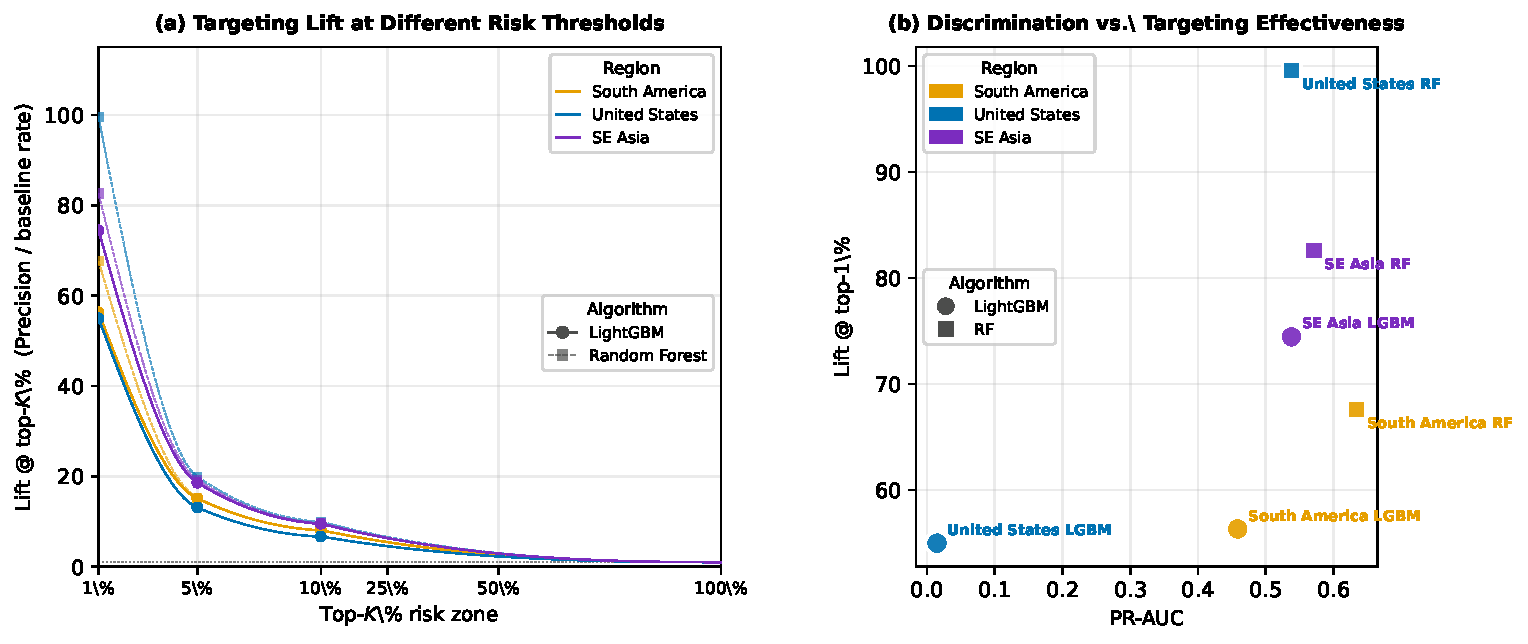
\includegraphics[width=\textwidth, keepaspectratio]{../outputs/south_america/results/model1_lgbm/model_comparison_landscape.pdf}
\caption{Cross-model performance comparison across all three regions (temporal test
set 2017--2019). \emph{Left:} Precision@$K$\% as a function of the top-$K$\% risk
threshold for LightGBM (solid) and Random Forest (dashed). Horizontal dotted lines
mark each region's baseline positive rate. The United States curve lies far below
the others because designation events are twenty times rarer than in South America or
Southeast Asia, yielding near-zero absolute precision despite strong rank
discrimination. \emph{Right:} ROC-AUC vs.\ Lift@1\% for all six model--algorithm
combinations; circles denote LightGBM, squares denote Random Forest.}
\label{fig:model_comparison_landscape}
\end{figure}

% ---------------------------------------------------------------------------
\subsection{Forward Projection (2025--2030)}
\label{sec:results_forward}

\subsubsection{Model Stability}
\label{sec:results_scatter}

Before presenting forward projections, the deployment model (trained on 2001--2019)
is compared with the evaluation model (trained on 2001--2016) to verify that
extending the training window does not destabilise the learned risk surface. If the
two models assigned substantially different rankings to the same pixels, the forward
projections would reflect training-data sensitivity rather than genuine geographic risk.

The per-pixel Pearson correlation between evaluation-model and deployment-model scores
across South America is $r = 0.36$ ($n = 46.8$~million pixels). This moderate
correlation is driven by the near-zero probability mass shared by the vast majority
of pixels in both models; for the decision-relevant upper tail (top 1\%), the
overlap between the two models' high-risk zones (Jaccard index) better characterises
stability and is reported in Appendix~\ref{app:backtest}. The sign of the correlation
is strongly positive, confirming directional consistency: pixels ranked high by the
evaluation model remain high-risk under the deployment model. The backtesting
validation in Appendix~\ref{app:backtest} provides the primary evidence of forward
procedure validity.
%TODO: NEEDS COMPUTATION: report top-1% Jaccard / rank-correlation between evaluation and deployment model scores for South America.

For the United States, the analogous correlation is $r = 0.07$ ($n = 36.7$~million
pixels). This lower value reflects a statistical property of the US data rather than
model instability: with a positive rate of only 0.04\%, both models assign near-zero
calibrated probabilities to the vast majority of pixels. Pearson correlation on a
distribution concentrated near zero is dominated by numerical differences in the tail
that do not necessarily reflect different risk orderings. The evaluation model's strong
Lift@1\% of 81.3$\times$ and recall@1\% of 81.4\% confirm that the top-ranked pixels
are genuinely enriched for future designations, and the spatial concentration of
high-risk predictions in historically active designation areas (federal lands in the
Southwest and Pacific Northwest) is consistent across both models. Forward projections for the United States are best interpreted as spatial
\emph{rankings} of transition risk rather than precise probability estimates.
For financial risk applications in the US context, the model provides a relative
risk ordering (which parcels are higher-risk than others) but not calibrated
absolute probabilities with the same reliability as for South America; users
should account for this when applying the US risk scores to portfolio-level
expected-loss calculations.

\subsubsection{30$\times$30 Tracking}
\label{sec:results_ontrack}

Table~\ref{tab:ontrack} summarises the current protection level, the business-as-usual
(BAU) trajectory, and the implied gap to the 30\% target for each region.

\begin{table}[H]
\centering
\caption{On-track assessment for the 30$\times$30 target based on formal WDPA PA
coverage only (OECMs excluded). Target~3 compliance counting OECMs and indigenous
conserved territories would show higher current coverage. BAU extrapolates the
2019--2024 designation rate forward. Shortfall is expressed as additional years
from 2024 to reach 30\% at the BAU rate.}
\label{tab:ontrack}
\begin{tabular}{lcccc}
\toprule
\textbf{Region} & \textbf{Coverage} & \textbf{Gap to 30\%}
  & \textbf{BAU rate (pct.\ pts./yr)} & \textbf{Shortfall} \\
\midrule
South America & 25.6\% & 4.4\% & 0.065 & $\sim$68 yr to target \\
United States & 7.7\%  & 22.3\% & $<$0.13 & $>$170 yr to target \\
Southeast Asia & 14.0\% & 16.0\% & $<$0.09 & $>$170 yr to target \\
\bottomrule
\end{tabular}
\end{table}
The BAU rate of 0.065 pp/yr used in the table is the average over 2019--2024; the
figure caption uses 0.061 pp/yr (the trailing 3-year average), resulting in a minor
discrepancy; both yield the same qualitative conclusion.

Under the business-as-usual scenario, no region is on track. South America faces the
smallest gap, having already reached 25.6\% protection, but even at its recent
designation pace it would not reach 30\% until approximately 2092 (approximately
68 years from 2024, or roughly 62 years past the 2030 deadline). The United States
and Southeast Asia face far larger deficits: both would require more than 170
additional years at current rates.

Figure~\ref{fig:sa_pa_coverage} places these trajectories in historical context,
showing how cumulative PA coverage in South America evolved from 2000 to 2024 and
what each scenario implies for the remaining path to 30\%.

\begin{figure}[H]
  \centering
  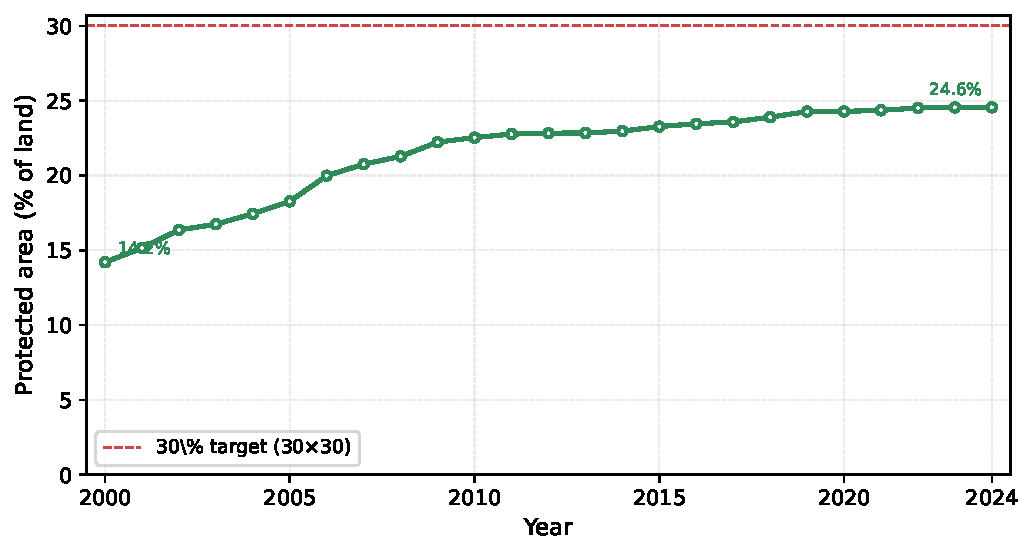
\includegraphics[width=0.75\textwidth, keepaspectratio]{../outputs/south_america/figures/WDPA_vis/sa_pa_coverage_pct.pdf}
  \caption{South America: cumulative protected-area coverage (2000--2024) with
  scenario projections to 2030. Historical data (circles) are from annual WDPA
  rasters. Dashed lines show three forward scenarios from the 2024 baseline
  (25.6\%): business-as-usual (BAU, +0.061\%/yr), moderate target (27.8\% by
  2030), and the 30$\times$30 target (30\% by 2030). Coverage grew rapidly
  during 2000--2013 and has plateaued well below the 30$\times$30 threshold;
  reaching the target requires a 12$\times$ acceleration relative to the BAU
  trajectory.}
  \label{fig:sa_pa_coverage}
\end{figure}

\subsubsection{Scenario Maps}
\label{sec:results_scenarios}

The forward model identifies spatially explicit priority areas under each scenario.
Under the 30$\times$30 scenario, the top-probability pixels are selected until the
cumulative area reaches 30\% of terrestrial coverage. Spatial
clustering on these highest-risk pixels identifies 40 distinct clusters in
South America (Figure~\ref{fig:forward_sa}), 39 in the United States, and 9 in
Southeast Asia. The relatively small cluster count in Southeast Asia reflects the geographic
structure of the region's risk surface: high-probability pixels are concentrated
in a handful of large, contiguous upland forest areas (Borneo highlands, Sumatra's
Bukit Barisan), producing a few large clusters rather than many small ones.

\begin{figure}[H]
\centering
\begin{subfigure}[t]{0.49\textwidth}
  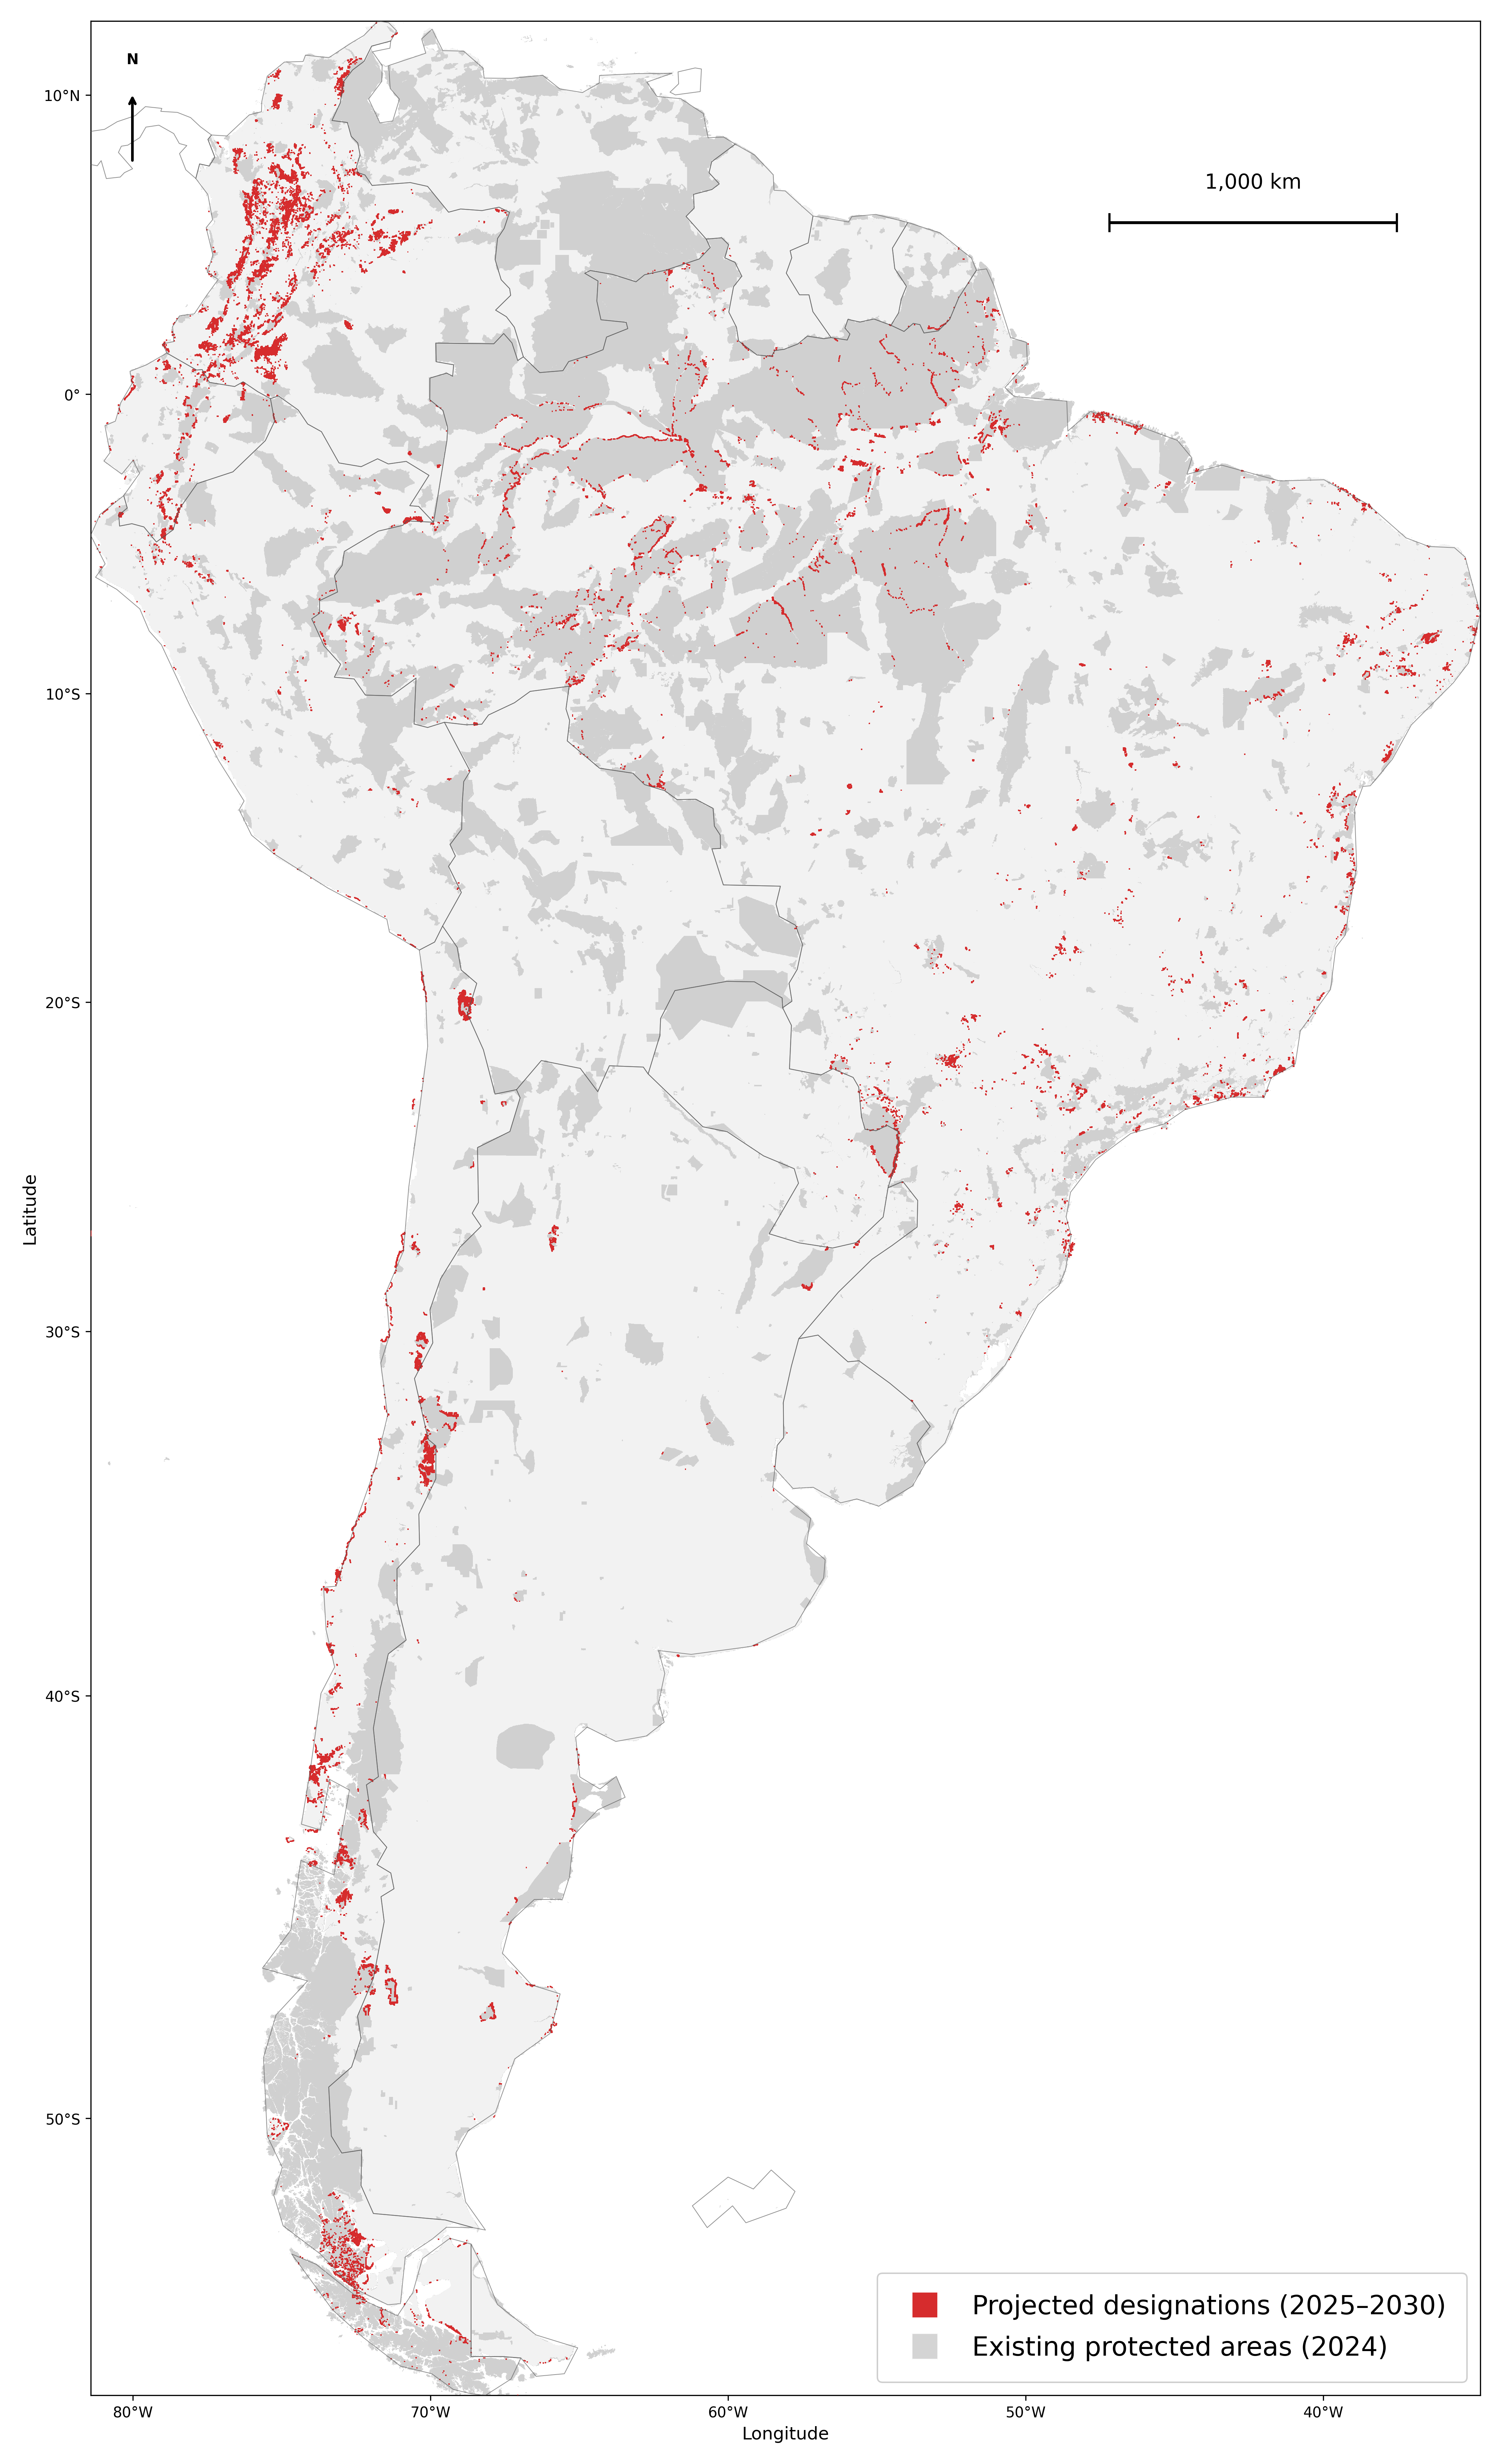
\includegraphics[width=\textwidth, keepaspectratio]{../outputs/south_america/results/forward/lgbm/risk_map_bau.png}
  \caption{Business-as-usual (BAU) scenario. Clusters show pixels designated if
  historical rates continue to 2030.}
  \label{fig:forward_sa_bau}
\end{subfigure}\hfill
\begin{subfigure}[t]{0.49\textwidth}
  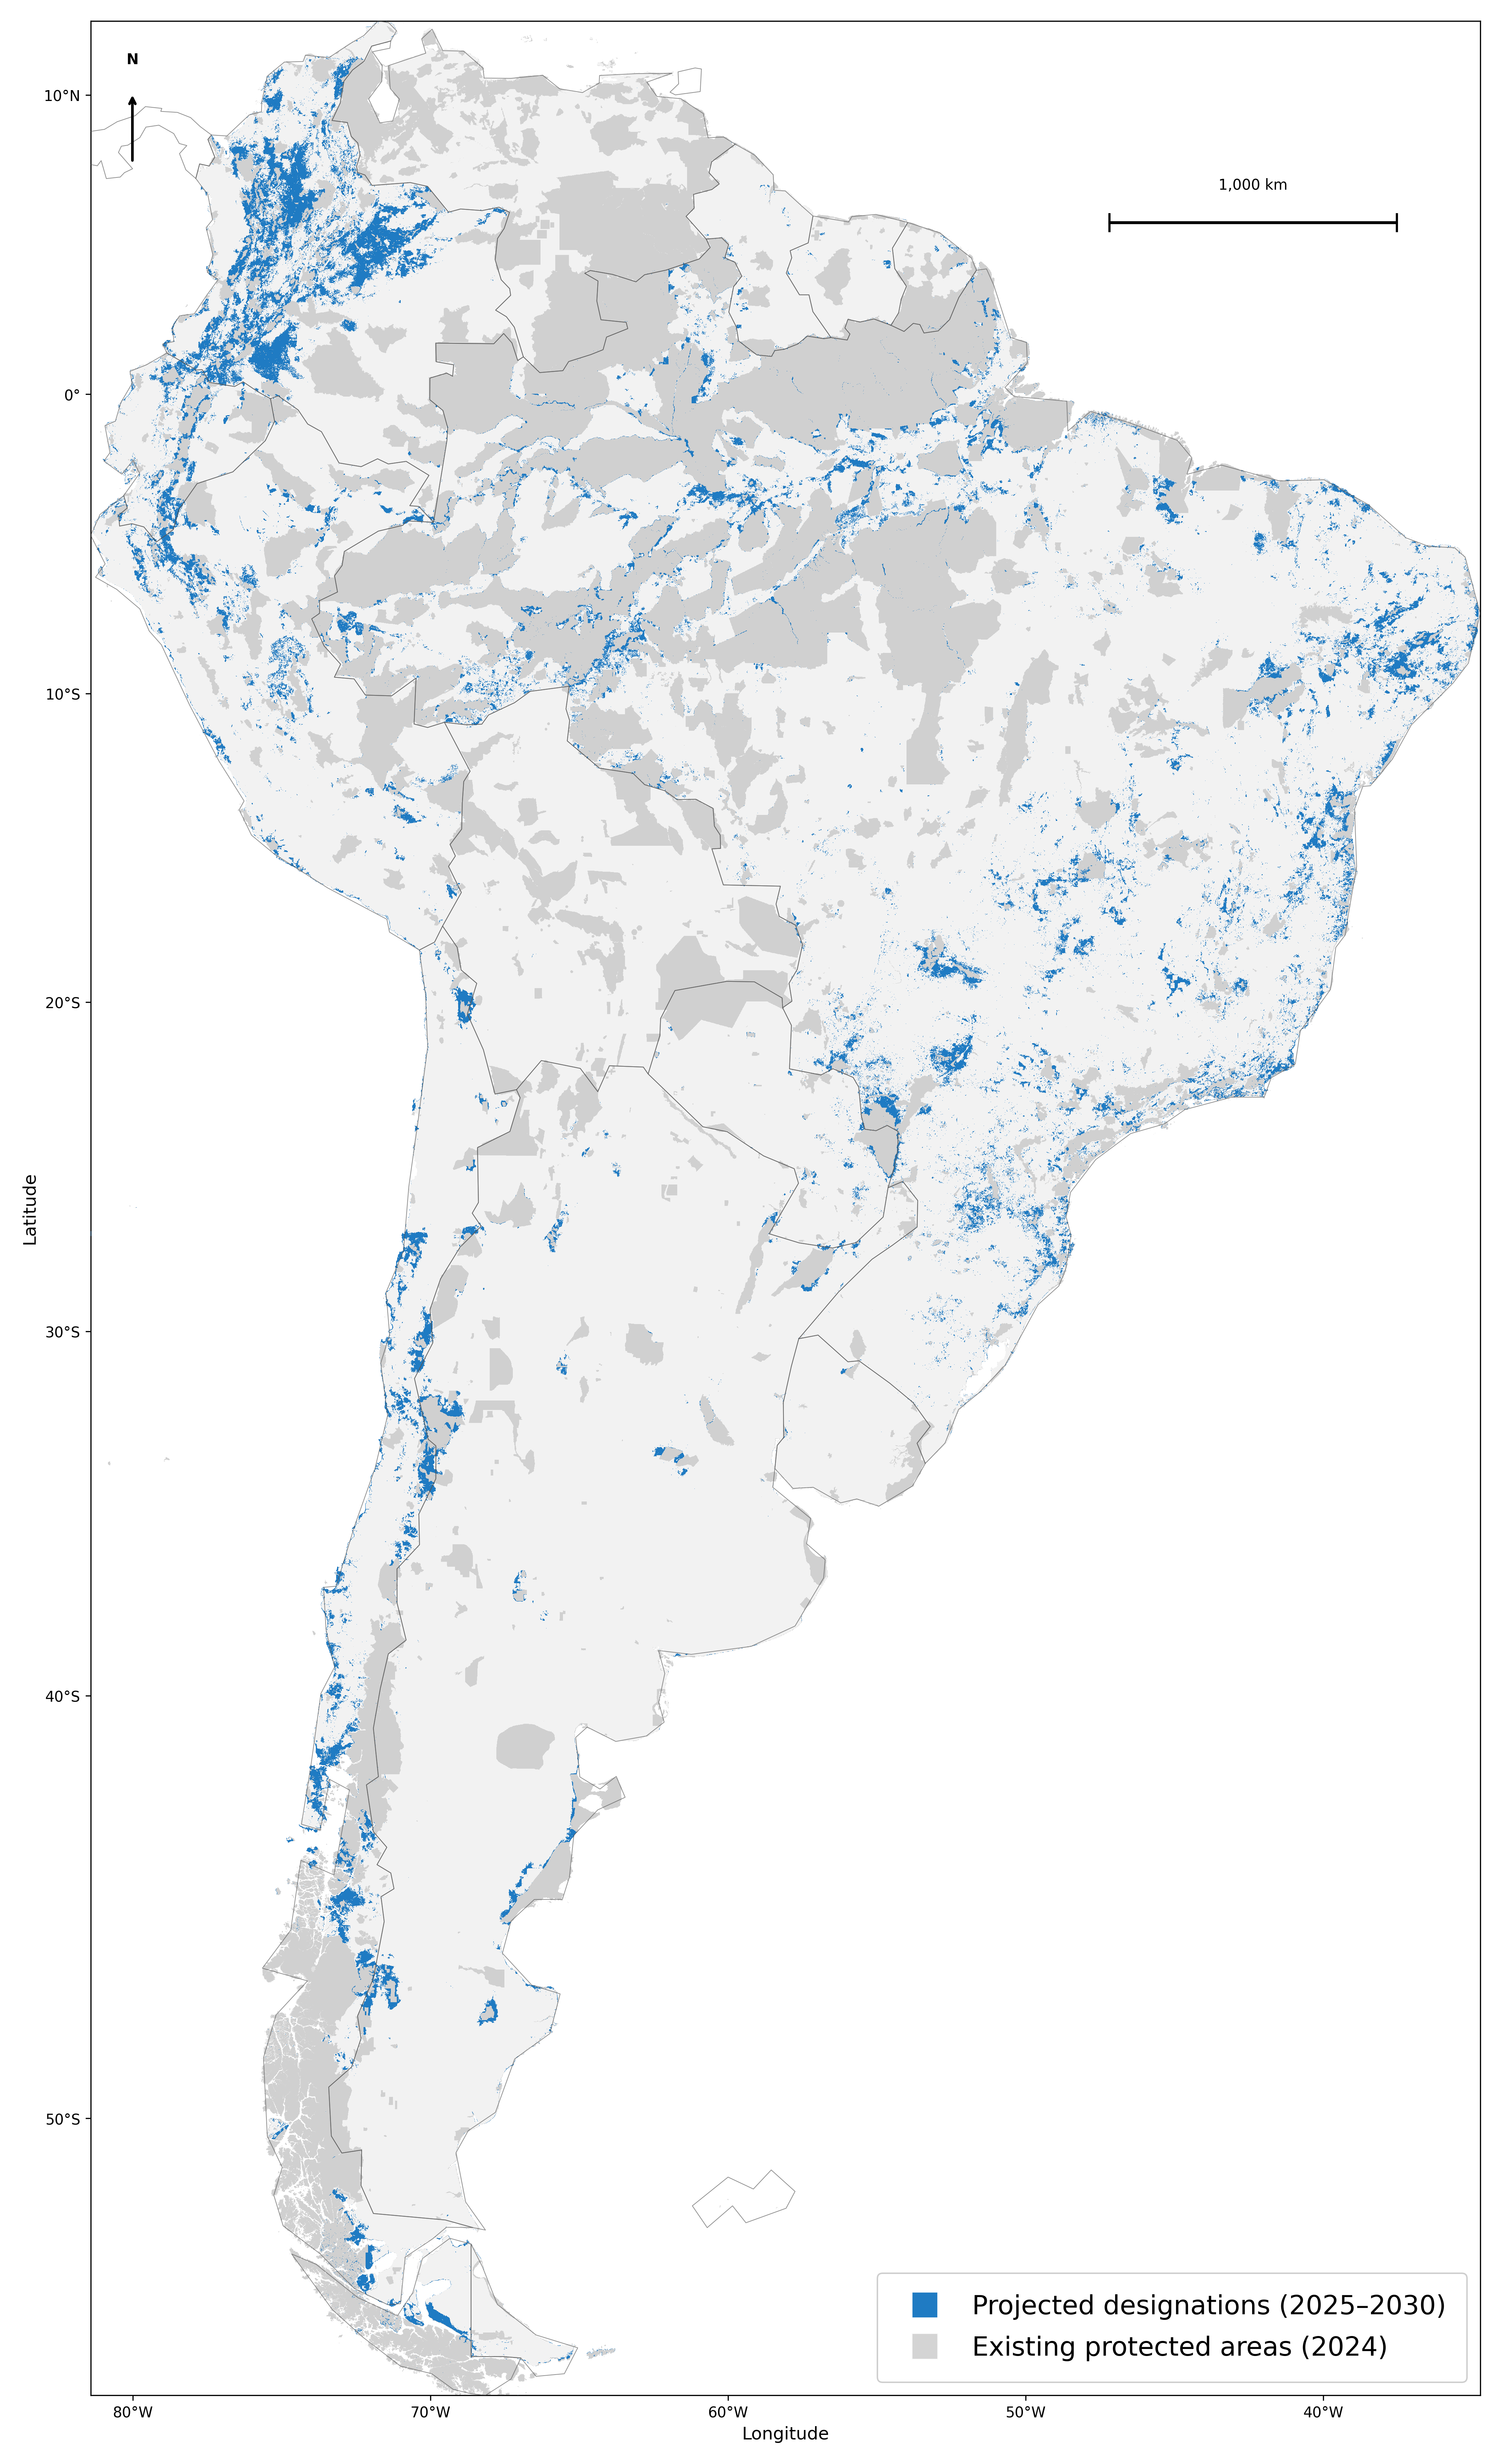
\includegraphics[width=\textwidth, keepaspectratio]{../outputs/south_america/results/forward/lgbm/scenario_30x30.png}
  \caption{30$\times$30 scenario. Clusters show the highest-probability pixels
  that would need to be designated to reach 30\% terrestrial coverage by 2030.}
  \label{fig:forward_sa_30x30}
\end{subfigure}
\caption{Forward projection for South America under the BAU and 30$\times$30 scenarios.
Coloured clusters indicate spatially contiguous groups of high-probability pixels;
grey shows the current protected-area network. Comparing the two panels illustrates
the additional designation pressure required to reach the 30$\times$30 target beyond
business-as-usual trajectories. Pixels are slightly enlarged for visual clarity.}
\label{fig:forward_sa}
\end{figure}

In South America, the highest-risk clusters concentrate in the Southern Amazon (Rondônia,
Mato Grosso, Pará), the Colombian Amazon, the Cerrado--Amazon transition zone, and the
Andes--Amazon piedmont. These are also the areas that have seen the most active designation
over 2015--2024. This convergence between predicted forward risk and recent historical patterns
is descriptively consistent with model continuity: since the deployment model's
training labels include five-year windows extending through 2024, this comparison
is not an independent out-of-sample validation. The walk-forward backtests
(Appendix~\ref{app:backtest}) provide the primary independent validation evidence.
Zoomed panels for the two highest-ranked South America clusters are shown in
Figure~\ref{fig:hotspot_sa} (Appendix~\ref{app:supp_figures}), illustrating the
spatial coherence of predicted designation pressure at sub-national scale.
The zoomed panels illustrate the sub-national precision of the model's risk surface;
they are provided in the appendix to keep the main text concise.

The United States clusters (Figure~\ref{fig:forward_usa}, Appendix~\ref{app:supp_figures}) concentrate in the Desert
Southwest (Arizona, Nevada, Utah), the Pacific Northwest, and the Southeast, areas
with large areas of Bureau of Land Management and National Forest land that
historically receive new wilderness and monument designations.

Southeast Asia clusters (Figure~\ref{fig:forward_seasia}, Appendix~\ref{app:supp_figures}) are concentrated in
northern and central Borneo, Sumatra's Bukit Barisan range, and the Philippines'
mountain biomes.

% [NOTE: Figure showing historical and projected designation pace by scenario available if needed]

\subsubsection{Economic Exposure}
\label{sec:results_exposure}

The forward model's risk surface is a potential input for transition-risk analysis.
To quantify the economic stakes, the area of agricultural land falling within the
top-1\% and top-5\% predicted risk zones is computed using MODIS land-cover
classifications applied to the forward-scored pixel set. Because the 1~km$^2$ cell is the modelling unit of the analysis (not the minimum legal
unit of PA designation, which can be smaller or irregular), each pixel's risk score
can be aggregated over any larger unit of interest,
such as a farm boundary, a watershed, or a lending portfolio, simply by averaging or summing
constituent cell scores.

The denominator for the top-1\% zone differs across the thesis: 208,000~km$^2$
(1\% of all 20.8M grid cells), 159,000~km$^2$ (1\% of the 15.9M test-period eligible
cells), and 138,000~km$^2$ (1\% of the 13.8M forward-scored eligible cells after
additional protected pixels are removed by 2024). The forward exposure analysis uses
the last figure, consistent with the deployment snapshot.

In South America, 582~km$^2$ of agricultural land falls within the highest-risk 1\% of
forward-scored unprotected pixels ($\approx 138{,}000$~km$^2$ total); the low share ($0.4\%$ of the
top-1\% zone) reflects the dominance of remote forested and shrubland pixels in the
high-risk zone, consistent with the opportunity-cost mechanism documented in
Section~\ref{sec:results_sa_shap}: land with high agricultural value is actively
suppressed from high-risk zones by the model. Widening to the top-5\% zone raises
the agricultural exposure to 6{,}143~km$^2$ (0.9\% of that zone), still modest,
confirming that in South America the transition-risk premium falls predominantly on
natural land.

In the United States, 9{,}949~km$^2$ of agricultural land falls within the top-1\%
risk zone ($\approx 73{,}000$~km$^2$ total; 13.6\% agricultural share), substantially
higher than South America's 0.4\%. The top-5\% zone raises this to 115{,}620~km$^2$
(32.3\%), reflecting the extensive mixture of private agricultural land and federal
public land across the American West. This cross-regional contrast is substantively important: in the US, designation risk
co-occurs with agricultural activity at a much higher rate. Note that the figures
reported are \emph{area} of agricultural land at risk, not monetary exposure; to
quantify financial materiality, these area estimates should be multiplied by
land value per km$^2$ or outstanding loan exposure.

In Southeast Asia, 37~km$^2$ falls within the top-1\% zone ($<0.1\%$), rising to
1{,}189~km$^2$ in the top-5\% zone (0.6\%), again reflecting the concentration of
high-risk pixels in remote forested uplands far from agricultural zones.
Table~\ref{tab:exposure} summarises these figures. Taken together, the consistently low agricultural shares for South America and
Southeast Asia are consistent with the SHAP finding that agricultural value
suppresses designation. For an independent check: among \emph{observed}
test-period (2017--2019) PA designations in South America, the share falling on
MODIS-classified agricultural pixels is below 2\%, corroborating that actual
designations also avoided agricultural land. The US exception reflects the
importance of federal land tenure in that context.

\begin{table}[H]
\centering
\caption{Agricultural land exposed to designation risk in the top-1\% and top-5\%
risk zones, by region (LightGBM forward model; MODIS land-cover). ``Share'' is the
fraction of the respective risk zone classified as agricultural.}
\label{tab:exposure}
\begin{tabular}{lrcrrc}
\toprule
 & \multicolumn{2}{c}{\textbf{Top-1\% risk zone}} & \phantom{ab} & \multicolumn{2}{c}{\textbf{Top-5\% risk zone}} \\
\cmidrule{2-3}\cmidrule{5-6}
\textbf{Region} & \textbf{Agri.\ area} & \textbf{Share} & & \textbf{Agri.\ area} & \textbf{Share} \\
\midrule
South America  & 582~km$^2$      & 0.4\%  & & 6{,}143~km$^2$   & 0.9\% \\
United States  & 9{,}949~km$^2$  & 13.6\% & & 115{,}620~km$^2$ & 32.3\% \\
Southeast Asia & 37~km$^2$       & $<$0.1\%  & & 1{,}189~km$^2$   & 0.6\% \\
\bottomrule
\end{tabular}
\end{table}

\subsubsection{Ecological Alignment}
\label{sec:forward_overlap}

The representation gap --- the divergence between \emph{where governments will
designate} and \emph{where designation is most ecologically important} --- is
quantified by overlaying the 30$\times$30 scenario map against two GSN priority
layers: high-biodiversity areas (\texttt{GSN\_b2}) and climate-stabilisation
priority areas (\texttt{GSN\_b1}). Because GSN layers are also predictors in the
model, this is a \emph{GSN-alignment} assessment rather than a fully independent
ecological validation; Key Biodiversity Areas or IUCN Red List range maps would
provide a more independent benchmark.

Under the 30$\times$30 scenario (the full target coverage allocation), only 18.4\% of projected designations
(790,202~km$^2$ total) fall within GSN biodiversity priority zones, and these designations
would cover just 4.9\% of the full biodiversity priority area (2,992,096~km$^2$).
The \emph{sweet spot} — land that is both projected for designation and classified as
biodiversity-priority — amounts to 145,154~km$^2$. The overlap with climate-stabilisation
priority areas is even smaller: only 1.1\% of projected designations intersect these zones,
covering 3.7\% of the climate-stabilisation priority area (227,777~km$^2$), with a sweet
spot of 8,539~km$^2$.

Figure~\ref{fig:alignment} maps these overlaps spatially. The concentration of
high-risk pixels along already-protected frontiers in the Amazon and Cerrado largely
misses the interior high-biodiversity zones of the western Amazon, the Atlantic
Forest remnants, and the Cerrado hotspots that remain critically underprotected.
This is consistent with the qualitative argument in Section~\ref{sec:discussion}:
expansion following historical patterns will not close the GSN-alignment gap. For
context, the current PA network covers 35.4\% of the full GSN biodiversity priority
area in South America (a random coverage model would cover 25.6\% at current
protection levels), suggesting the existing PA network already overrepresents
biodiversity-priority land relative to random; the projected 30$\times$30 expansion
would reduce this overrepresentation by concentrating new designations in lower-priority land.

\begin{figure}[H]
  \centering
  \begin{subfigure}[t]{0.49\textwidth}
    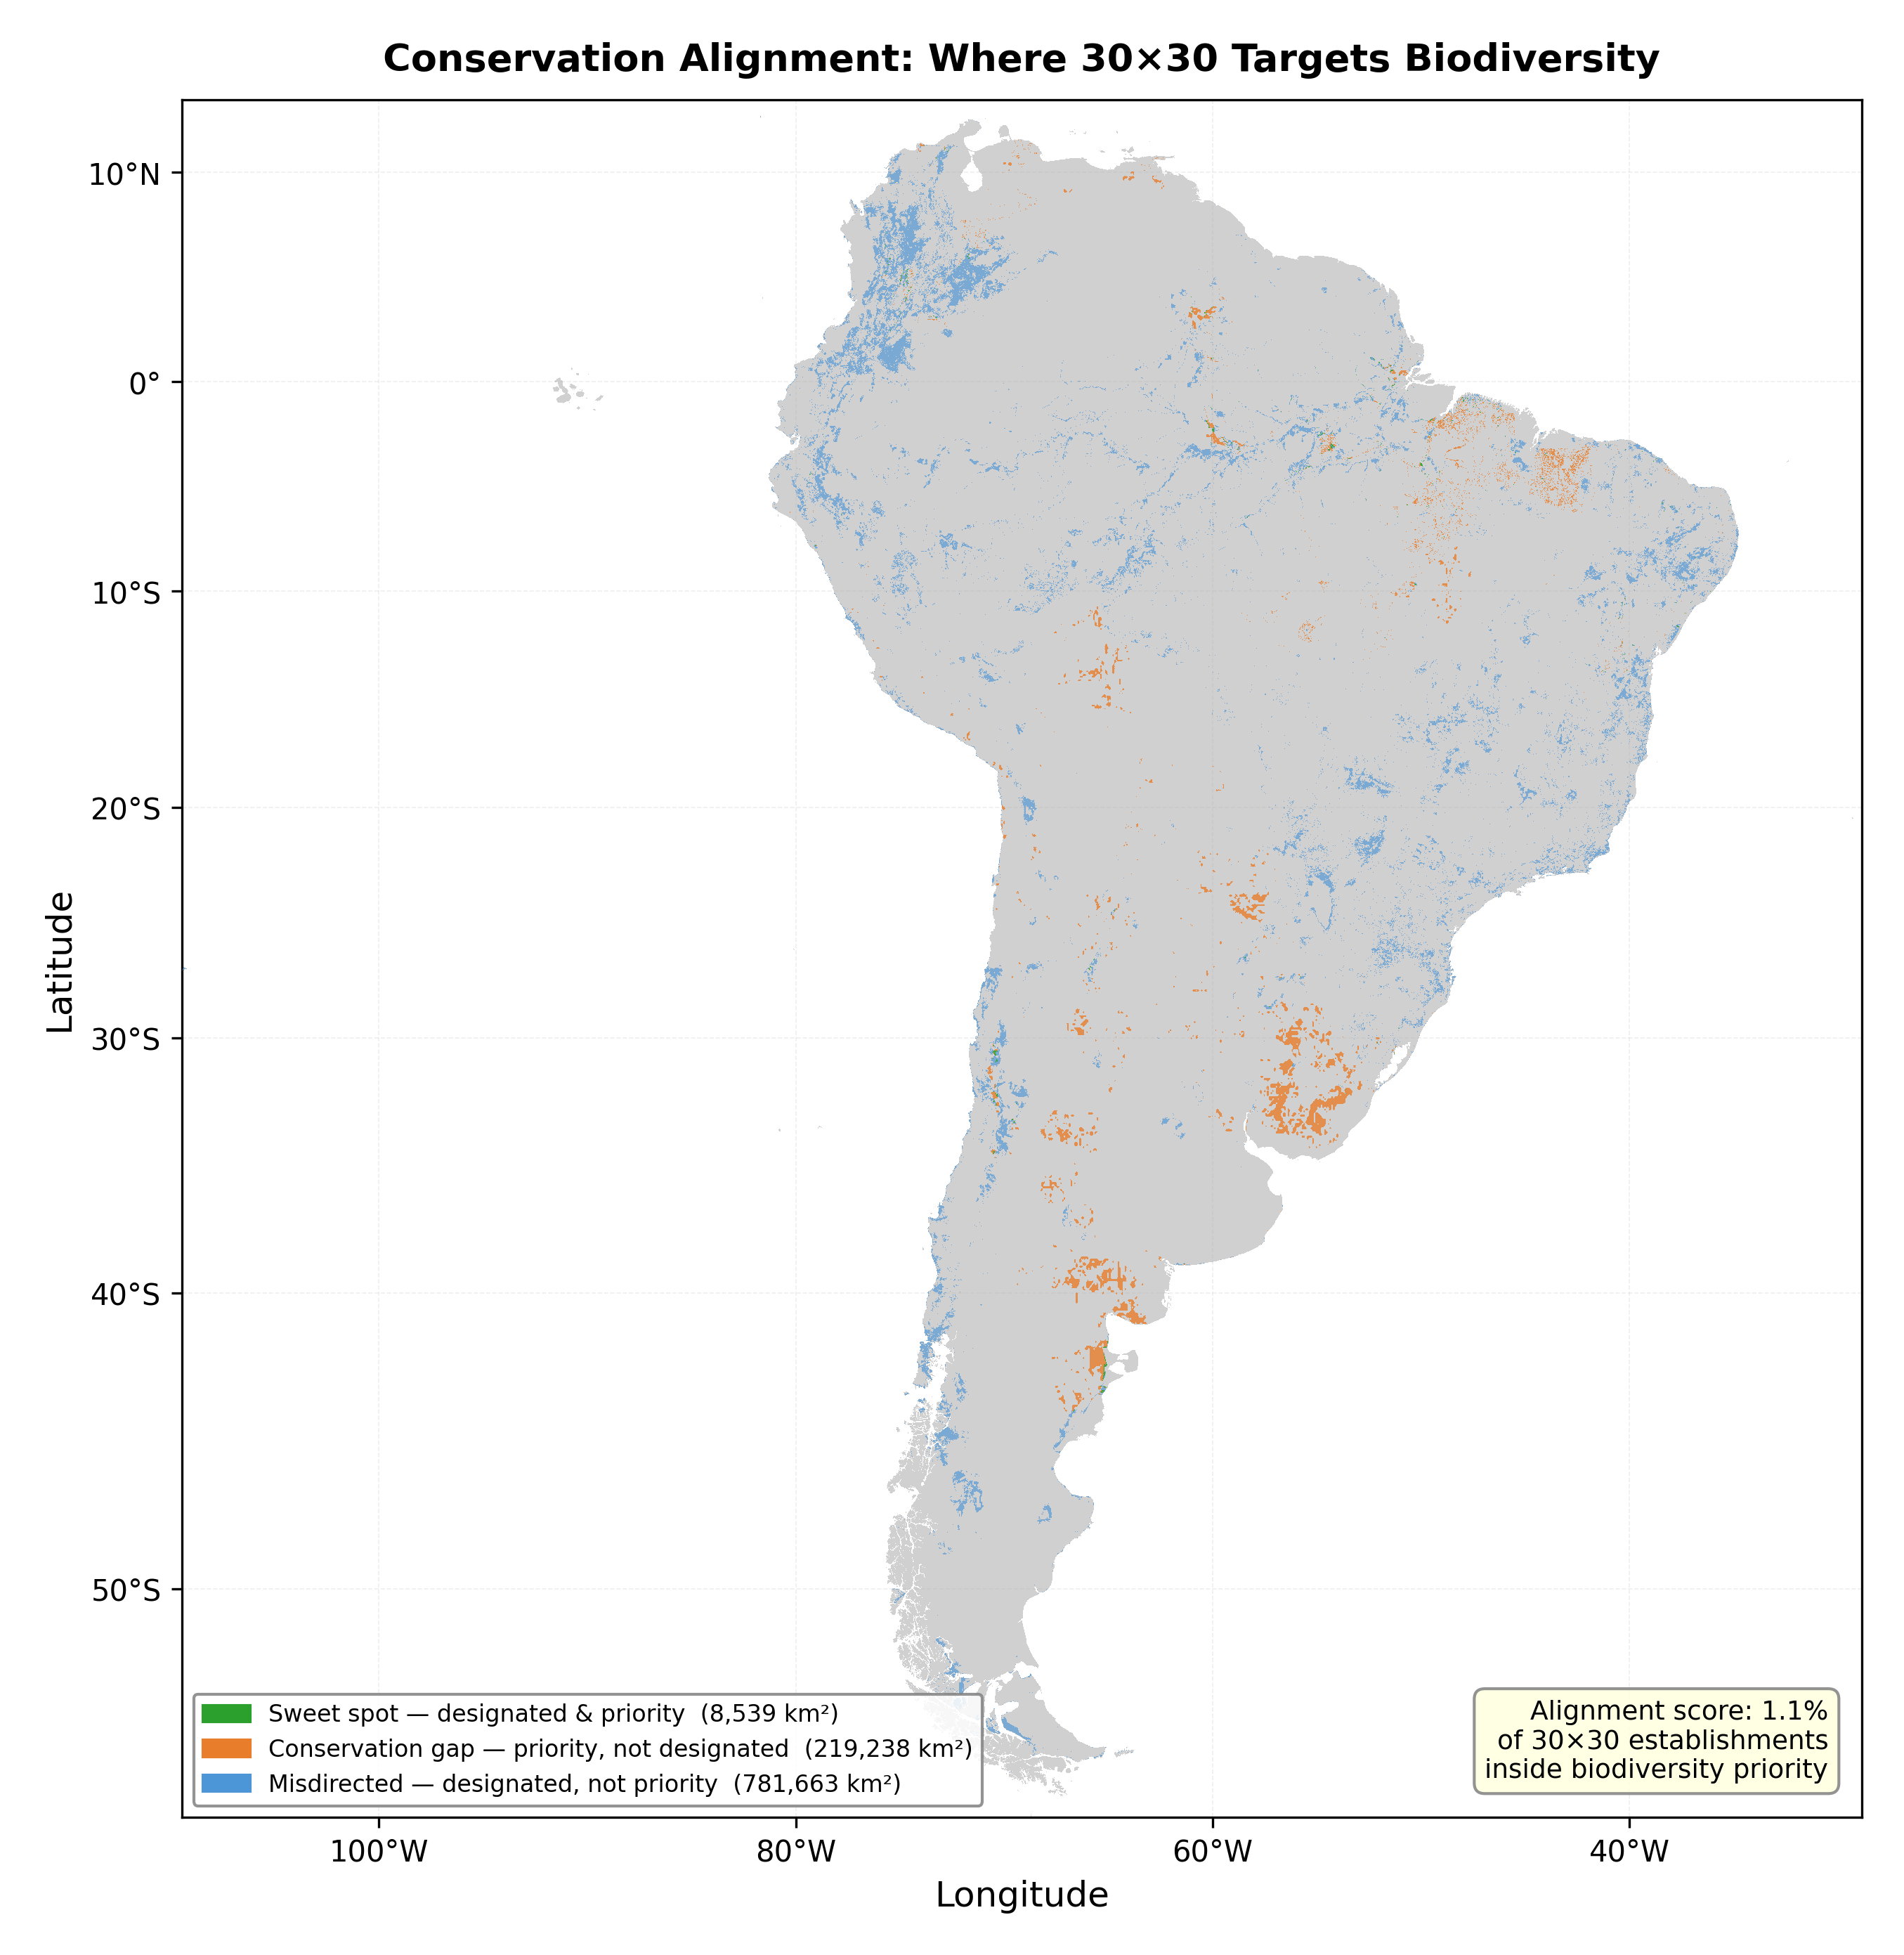
\includegraphics[width=\textwidth, keepaspectratio]{../outputs/south_america/results/forward/lgbm/conservation_alignment.png}
    \caption{Biodiversity priority overlap\\
    \textit{\small Red: priority, not designated; Gold/Orange: designated, not priority; Blue: designated \& priority}}
    \label{fig:alignment_biodiversity}
  \end{subfigure}\hfill
  \begin{subfigure}[t]{0.49\textwidth}
    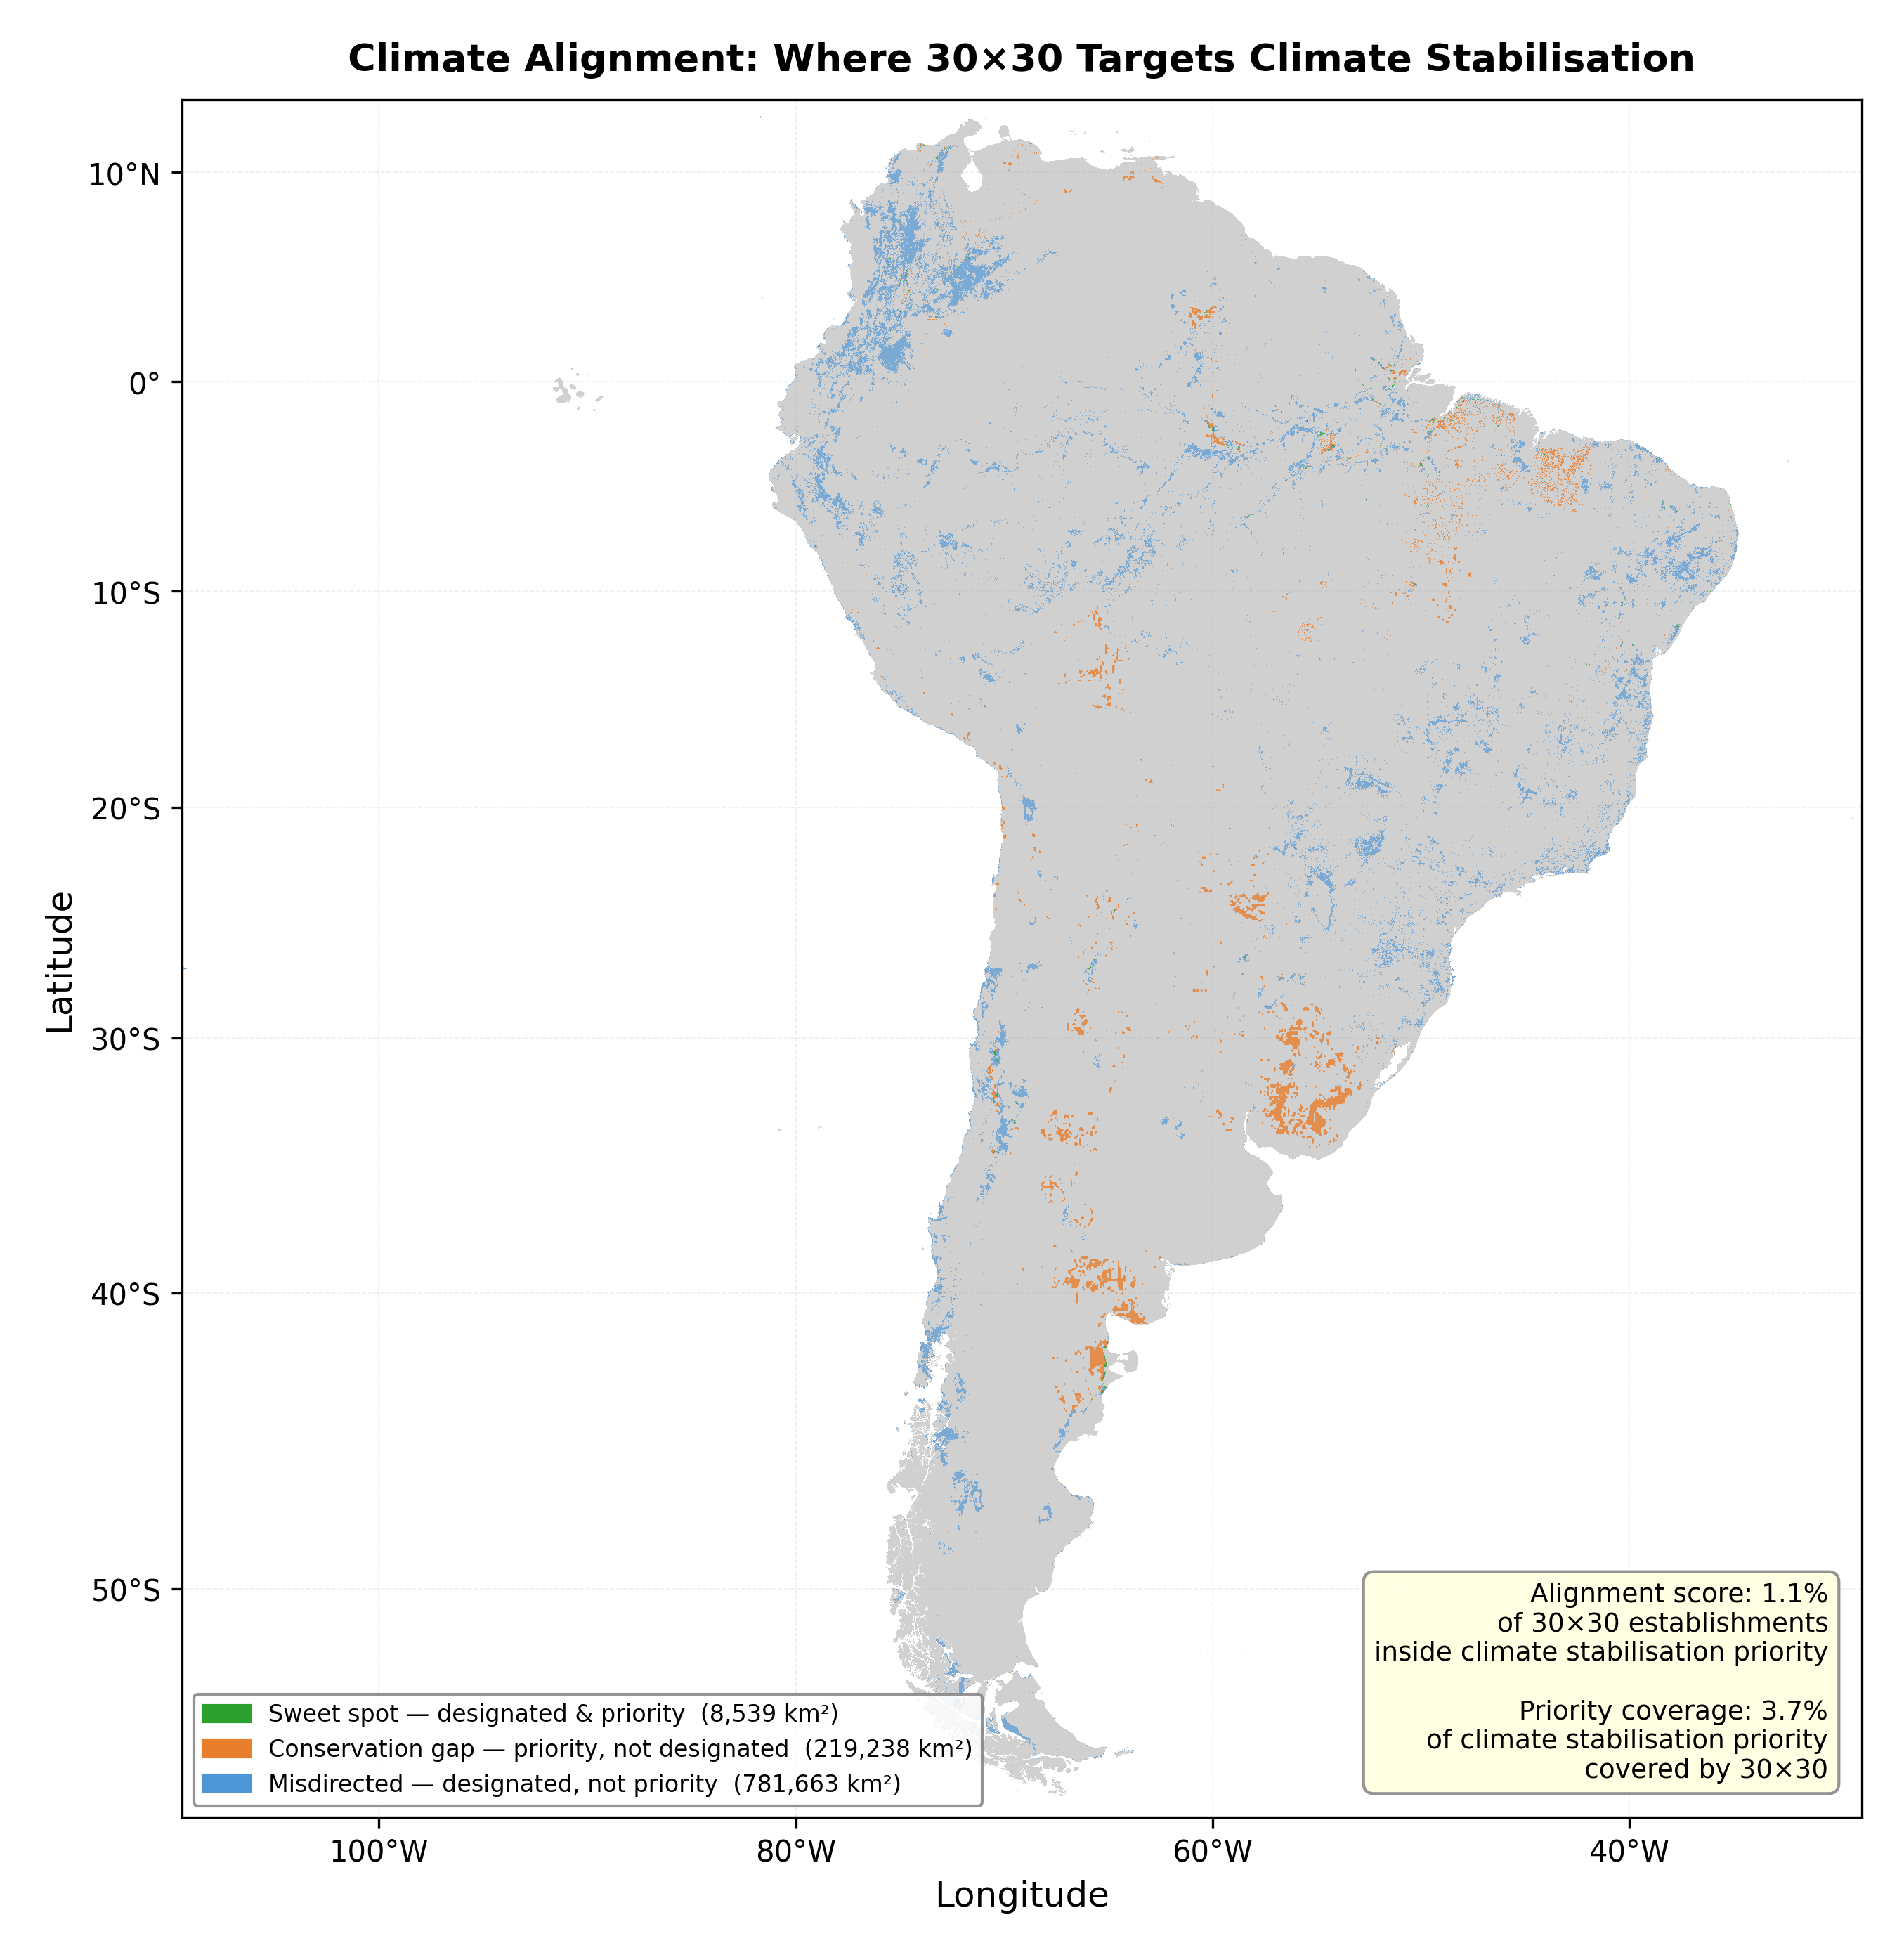
\includegraphics[width=\textwidth, keepaspectratio]{../outputs/south_america/results/forward/lgbm/climate_stabilisation_alignment.png}
    \caption{Climate-stabilisation priority overlap\\
    \textit{\small Red: priority, not designated; Gold/Orange: designated, not priority; Blue: designated \& priority}}
    \label{fig:alignment_climate}
  \end{subfigure}
  \caption{Overlap between projected 30$\times$30 designations and GSN ecological
  priority areas in South America (LightGBM). Biodiversity-priority overlap: 18.4\%;
  climate-stabilisation overlap: 1.1\%. Path-of-least-resistance expansion
  does not target the most ecologically critical land.}
  \label{fig:alignment}
\end{figure}

% ===========================================================================
%  Discussion
% ===========================================================================
\section{Discussion}
\label{sec:discussion}

\subsection{Driver Hierarchy and Designation Politics}
\label{sec:disc_drivers}
The SHAP analysis suggests a driver hierarchy in which biodiversity value and
governance quality are the most influential predictors in the fitted model,
with economic opportunity cost entering as a secondary but substantive predictor.
A formal ablation study removing each predictor group in turn would provide stronger
evidence for this ordering; as it stands, the hierarchy rests on mean absolute SHAP
values and is subject to multicollinearity among groups. These are predictive
associations, not causal claims: the framework cannot
establish whether stronger governance causes higher designation rates, or whether
both reflect deeper country-level characteristics such as income or international
integration.
GSN conservation-priority indicators rank above all other variable groups;
governance indicators (WGI Rule of Law, V-Dem Liberal Democracy Index) rank second,
ahead of infrastructure-based proxies for economic activity. This is not the
purely cost-driven ``least-resistance'' story that early empirical work suggested
\citep{joppa2009, venter2018}: rather, institutional capacity to act on conservation commitments is a binding constraint
of comparable importance to economic opportunity cost. The two channels are
complementary rather than competing: regions combine all three conditions,
ecological priority, institutional capacity, and low economic cost, for the
bulk of their historical designations.

The implication for the 30$\times$30 target is therefore twofold. First, in
countries with weak institutions, even ecologically important areas may remain
unprotected not because they are economically valuable but because the state lacks
the administrative capacity to gazette and enforce new PAs. Second, in countries
with strong governance, the remaining unprotected biodiversity-priority land tends
to be economically valuable, requiring the compensation mechanisms (direct payments,
conservation easements, carbon market incentives) that are central to the political
economy of ambitious designation. If future designations follow the same
governance-and-ecology logic as historical ones, the additional 12 percentage
points of coverage will concentrate in countries with both strong institutions and
available low-cost land, leaving biodiversity-rich areas in governance-constrained
contexts systematically underrepresented \citep{venter2018, eckert2023}. This governance-biodiversity mismatch is documented globally in the PA siting
literature \citep{venter2018, eckert2023}, with regions such as the Congo Basin and
Melanesia cited as examples where high-biodiversity forests sit in governance-constrained
countries; these regions are outside the empirical scope of this thesis and the
pattern is cited as background, not as a model result.

The SA PR-AUC of 0.645 (against a random baseline of 0.008) is of a similar order
to the discrimination achieved by \citet{mouillot2024} using a comparable
socio-environmental niche approach. Direct comparison requires caution:
\citet{mouillot2024} model the current spatial distribution of PAs (a cross-sectional
classification task) rather than future transitions (a prospective forecast), and
the metrics are not directly comparable; the figure is offered as contextual
evidence that geographic and institutional covariates contain sufficient signal to
characterise PA designation at continental scale.

\subsection{Representation Gap}
\label{sec:disc_representation}
The LOBO analysis reveals a predictable pattern of biome underrepresentation under
historical dynamics. Biomes with high LOBO performance are those where designation
follows consistent geographic gradients: in South America, temperate and tropical
forests with distinctive elevation and remoteness signatures generalise well across
biome boundaries, while certain tropical dry biomes achieve high lift owing to very
low positive rates. Biomes with poor LOBO performance exhibit idiosyncratic
designation patterns driven by institutional and political factors: temperate conifer
forests in the US and flooded grasslands and tropical savannas in South America show
near-random or below-random lift, indicating that the static geospatial feature set
cannot capture the seasonal, tenure-based, or agreement-driven processes that govern
designation in those ecosystems.

This suggests a representation gap: biomes with poor LOBO performance show that
historical patterns do not apply consistently across ecological contexts, and the
GSN alignment analysis (Section~\ref{sec:forward_overlap}) shows that only 18.4\%
of projected 30$\times$30 designations overlap with biodiversity priority zones.
Together, these results indicate that even if 30\% terrestrial coverage is achieved,
the distribution across biomes is likely to remain biased toward ecologically
``easy'' land. Closing this gap requires active policy intervention: conservation
finance instruments, direct payments, or binding biome-specific targets.

The economic exposure results (Section~\ref{sec:results_exposure}) reveal the
converse dimension of this gap. In South America and Southeast Asia, the high-risk
zone is overwhelmingly composed of remote forest, shrubland, and savanna: areas that
are both ecologically valuable and economically cheap to designate, which is precisely
why they score highly under historical designation patterns. The agricultural share of the top-1\% risk zone is below 1\% in both regions.
Low agricultural share implies natural land dominance, but not automatically
ecological relevance: the GSN alignment analysis (18.4\% overlap with biodiversity
priority zones) shows that only a minority of high-risk natural land falls within
globally prioritised conservation areas. The
designation risk for agricultural landowners is therefore concentrated at the edges of
these natural landscapes, not at the core. In the United States, by contrast, the
top-1\% zone has a 13.6\% agricultural share, reflecting the mixed public-agricultural
landscape of the West where ecological and economic use coexist. Here the predicted
designations are less purely ``ecologically easy'' and carry a higher direct cost to
working agricultural businesses, which also makes them more politically contested.

\subsection{Cross-Continental Limits}
\label{sec:disc_transfer}
Cross-continental transfer performance varies markedly by algorithm (full results in
Table~\ref{tab:transfer_full}, Appendix~\ref{app:transfer}). For LGBM, transfer is
near-random or below-random in most directions (SA$\to$USA: 0.517; USA$\to$SA: 0.518;
SE Asia$\to$USA: 0.238; SE Asia$\to$SA: 0.381). For RF, several directions show
substantial transfer (SA$\to$SEA: 0.720; SEA$\to$USA: 0.713; SEA$\to$SA: 0.598),
indicating that the RF's bagged architecture captures more transferable ecological
baselines while LGBM overfits more strongly to regional institutional patterns.
Protected-area designation is \emph{institutionally specific}: its spatial pattern
is not a universal law derivable from physical geography but a product of specific
national legal frameworks, political histories, and institutional capacities \citep{ludwig2023}.
Even a feature set that includes both remotely-sensed covariates and country-level
governance indicators cannot capture the specific congressional acts that create
a national monument in Utah or the presidential decrees that establish Amazonian
reserves, because the \emph{mapping} from general institutional quality to specific
spatial designation patterns differs fundamentally across governance regimes.

This finding has two practical implications. For risk assessment, it confirms that
region-specific models are required: a single global risk score would obscure
continent-level variation in the drivers of designation. For LGBM-based risk scoring, the evidence supports region-specific models; whether
a global hierarchical model with tenure and country fixed effects could achieve
comparable performance has not been tested. For research, the findings suggest
that the most valuable next-generation features are spatially granular institutional
ones: parcel-level land-tenure status (public vs.\ private ownership), which country-level
governance indicators cannot proxy, carbon-market eligibility at the project level,
and NGO funding flows that enable or constrain specific designation processes.

\subsection{Calibrated Risk Scores}
\label{sec:disc_calibration}
The core value proposition of this framework for financial risk applications depends
on calibration. A raw ranking of pixels by predicted score is useful for conservation
prioritisation, but transition-risk quantification requires statements of the form
``this parcel has a 3\% probability of being designated within five years'': an
interval-scale probability, not an ordinal rank.

After Platt scaling, the ECE of 0.0081 in South America confirms that the calibrated
scores have this property: on average, the predicted probability deviates from the
observed transition rate by less than one percentage point across the score distribution.
A lender extending a five-year agricultural loan secured on land with calibrated
$\hat{p}$ could compute a simple expected transition loss as
$\hat{p} \times \text{EAD} \times \text{LGD}$, where EAD is the exposure at default
and LGD is the loss given designation (e.g.\ the agricultural land value discount
under PA restrictions), analogous to credit expected-loss calculations. This
application is conceptually straightforward but has not been demonstrated with real
loan data; it represents a natural next step for practitioners adopting the risk maps.

The model produces a conditional forecast, not an unconditional one: probabilities are
calibrated to historical designation patterns and assume that the policy environment
does not change structurally. If the Kunming-Montreal commitments trigger a sustained
acceleration in designation pace, calibrated probabilities would underestimate true
risk. Under the assumption that 30$\times$30 political momentum persists and accelerates
designation, the BAU scenario could understate true risk; but designation momentum
could also stall, reverse through legal challenge, or shift to OECMs not counted
in this framework. The BAU scenario is therefore best interpreted as a central
reference trajectory, not a bound.

A potential second-order effect, worth noting as a hypothesis for future work, is
that large-scale PA expansion could raise the value of remaining undesignated
agricultural land by increasing its effective scarcity; this scarcity-premium
mechanism is documented in land-market theory \citep{geoghegan2002} but has not
been estimated in the 30$\times$30 context. Practitioners using the risk maps should
note that the calibrated probabilities capture only the direct designation risk
channel.

\subsection{Forward Projection and Policy}
\label{sec:disc_forward}
The on-track assessment in Table~\ref{tab:ontrack} delivers a clear message: no region
studied here will reach the 30$\times$30 target on time under business-as-usual
trajectories. South America, despite having the smallest percentage-point gap, would require
approximately 68 additional years from 2024 to reach 30\% at BAU rates (or roughly
62 years past the 2030 deadline); the United States and Southeast Asia face
deficits of more than 170 additional years. All figures refer to formal WDPA PA
coverage; counting OECMs and indigenous territories toward Target~3 would reduce
these shortfalls.

Closing this gap requires not only more designations but also different designations.
The scenario maps identify which specific geographic clusters would need to be
designated under each pathway. Governments committed to the 30$\times$30 target can
use these maps in two complementary ways. First, as a prioritisation tool: the
high-probability clusters identify which areas are most consistent with historical
designation patterns and thus most politically feasible to protect in the near term.
Second, as a gap analysis: comparing the scenario maps to GSN priority layers
(as done in Section~\ref{sec:forward_overlap}) reveals which high-priority areas
are \emph{not} predicted to be designated under the modelled trajectory; comparison
to Key Biodiversity Areas or IUCN Red List habitat maps would provide a more
independent benchmark and is a natural extension.

The distinction between governments that need to \emph{accelerate} designation and
those that need to \emph{redirect} it matters. South America needs primarily to accelerate; the US needs to accelerate substantially
more, and redirection toward ecologically higher-priority areas would require
overcoming the strong federal-land tenure bias identified in the LOBO analysis, though
an explicit GSN alignment analysis for the US has not been conducted.

\subsection{Limitations}
\label{sec:discussion_limitations}
The model extrapolates historical designation patterns forward and is subject to
a stationarity assumption. Structural breaks, such as a change in government, a new
carbon-market mechanism, the Kunming-Montreal momentum, or emerging nature-related
financial disclosure requirements \citep{tnfd2023}, are not modelled. Calibrated
probabilities should be interpreted as conditional forecasts: what would the five-year
designation probability be, given that the historical pattern continues? They are not
unconditional predictions of what will happen. For transition-risk applications,
conditional forecasts are the appropriate product; they answer the question investors
and lenders actually face: what is the risk given current trajectories? The BAU scenario should be read as a conditional reference trajectory, not a
lower bound. Post-COP15 political momentum could accelerate designations above the
BAU rate; equally, designation momentum could stall (political reversals, funding
shortfalls), legal rollbacks could reduce effective protection, or implementation
could shift toward OECMs and private conservation not captured by WDPA formal PAs.
The model does not model any of these scenarios explicitly.

The current feature set includes country-level governance indicators (WGI, V-Dem, DPI)
and indigenous territory boundaries (LandMark), but is missing key spatially granular
institutional variables: parcel-level land-tenure status (public vs.\ private
ownership) and carbon-market project eligibility (REDD+ credits). Country-level
governance quality imperfectly proxies the parcel-level tenure constraints that drive
many designation decisions, particularly in mixed federal-private landscapes such as
the US West. NGO funding flows, which directly enable specific designation processes,
are also unobserved. Incorporating parcel-level tenure data, where available, would be
the highest-priority extension.

Two data-quality issues affect the target variable. Gazette year entries in the WDPA
may lag the formal legal designation by one to three years in some jurisdictions
\citep{bingham2019}; the five-year lookahead window reduces sensitivity to small date
errors, but systematic lags in data entry could introduce a small bias toward later
observation of transitions. More structurally, the WDPA's increasing incorporation of
Other Effective Area-Based Conservation Measures (OECMs), which vary widely in
protection strength from strictly managed nature reserves to loosely governed community
areas, may introduce heterogeneity in the target variable not captured by the binary
protected/unprotected classification \citep{maxwell2020}.
OECMs and indigenous conserved areas often arise
precisely where conventional PA designation has not been politically feasible: in areas
with higher human pressure, active resource-use rights, or contested land tenure. A
model trained on historical WDPA entries dominated by classical PA types would not
learn the socio-environmental signature of OECM siting, and forward projections
calibrated to traditional PA patterns could systematically miss the areas most likely
to receive OECM designations under the Kunming-Montreal Framework.

Country-level composite indicators (WGI, V-Dem) and remotely sensed proxies (NDVI,
night-time lights) are measured with error relative to the true underlying quantities
they approximate. Measurement error attenuates estimated feature importance and can
reduce discrimination. Predictors measured with greater spatial precision would be
expected to improve discrimination, particularly in biomes where the current LOBO
performance is near-random. Relatedly, neighbouring pixels share similar covariate
values and often share designation outcomes because entire landscapes are designated
together. This spatial autocorrelation can inflate within-region evaluation metrics,
including LOBO, because training pixels from other biomes still contain information
correlated with the held-out biome through shared continental gradients in climate and
terrain. The LOBO framework mitigates this by holding out entire biomes, but cannot fully
eliminate it; users should interpret LOBO metrics as upper bounds on true
out-of-sample performance. Additionally, the 1~km$^2$ modelling unit introduces
a modifiable areal unit problem: designation outcomes at coarser resolution (e.g.\
2~km) or finer resolution (e.g.\ 500~m) could yield different performance estimates
and spatial risk patterns, and PA polygon boundaries do not align to a pixel grid.

Several methodological choices warrant sensitivity caveats. The distance-to-existing-PA
feature (\texttt{dist\_wdpa}) captures spatial path dependence but risks encoding a
subtle endogeneity: large protected areas are sometimes designated in successive
administrative steps over several years, so pixels immediately adjacent to an existing
PA may score highly simply because they are part of the same multi-year designation
process rather than because they are independently at risk. The one-year temporal lag
on \texttt{dist\_wdpa} mitigates but does not eliminate this concern. Temporal
weighting likewise introduces a modelling choice: observations in later training years
receive higher weight, and if the post-2010 acceleration in designation pace is a
temporary policy phase rather than a persistent structural shift, this weighting may
cause the model to over-extrapolate recent dynamics. Both sensitivities would require full continental-scale re-training runs to formally
test and are not conducted here due to computational resource constraints; this is
acknowledged as a study limitation. Additionally, road proximity and night-time
lights are strong predictors partly because they proxy accessibility, but also because
they correlate with economic development levels that independently influence the
political feasibility of protection; the model cannot separately identify these
mechanisms, and causal interpretation of the feature importance is therefore not
warranted.

The relative contribution of each predictor group has been characterised through SHAP
values, but a formal ablation study removing each group in turn and measuring the
change in PR-AUC has not been conducted. Ablation would provide stronger evidence that
the individual predictor groups independently add predictive value rather than acting
as proxies for one another, and remains a priority for future work.

Finally, pixels assigned high predicted probability that are not designated within the
five-year evaluation window are classified as false positives by conventional metrics.
However, spatial inspection of false positives from the walk-forward backtests
(Appendix~\ref{app:backtest}) reveals that a substantial share cluster along known
designation frontiers, in the same geographic corridors that received PAs in adjacent
time windows. Many false positives are therefore better characterised as ``right
prediction, wrong window'': the model correctly identifies them as elevated-risk zones,
but the designation is delayed beyond the five-year horizon. This is an inherent
constraint of the fixed-window binary target rather than a model failure. The
persistence of false positive clusters across independent backtest origins (2009, 2011)
provides indirect evidence that the forward risk maps are spatially consistent: the
same frontier zones recur as high-risk across all periods evaluated. A formal check
of whether these false positives subsequently transition in later WDPA releases
(i.e.\ were ``right prediction, wrong window'') has not been conducted and would
require matching the false-positive spatial footprint against 2025-onward WDPA
additions. Throughout, the framework is explicitly predictive, not causal: SHAP values should be read as partial correlations, not causal
effects, and the appropriate use of this framework is spatial risk screening and
portfolio prioritisation, not policy impact evaluation.

% ===========================================================================
%  Conclusion
% ===========================================================================
\section{Conclusion}
\label{sec:conclusion}

This thesis has developed and evaluated a machine-learning framework for predicting
the spatial expansion of protected areas under the 30$\times$30 biodiversity target,
applied to three major world regions. The primary model for South America achieves a ROC-AUC of 0.897 and captures 77.4\%
of all test-period PA establishment events within the top 1\% of predicted risk
(pixel-year Lift@1\% = 66.8$\times$; event-level Precision@1\% = 79.8\%), performance
sufficient to make the model a practically useful tool for spatial transition-risk
screening. Calibrated predicted probabilities serve as interval-scale transition-risk
scores that are a prerequisite input for financial risk quantification, portfolio
screening, and land-use planning; full portfolio aggregation workflows remain an
avenue for future applied work.

Three empirical findings emerge from the analysis. The driver hierarchy reveals
that conservation priority (GSN biodiversity indicators) and governance quality
(WGI Rule of Law, V-Dem Liberal Democracy Index) are the primary predictors of
where PAs are designated, not merely economic opportunity cost. If future
designations continue to follow the same governance-and-ecology logic as historical
ones, closing the 30$\times$30 gap will require strengthening institutions and
providing compensation mechanisms in biodiversity-rich, economically contested areas,
not only designating remote land. The gap between what this model predicts and where
designation \emph{should} go for maximum conservation impact is itself a policy
finding: it reveals where the 30$\times$30 commitment risks being met on paper
without delivering proportionate biodiversity outcomes. Forward projections reinforce the urgency: all three studied regions are severely
off-track, South America by approximately 68 additional years from 2024 and the
United States and Southeast Asia by more than 170 additional years at current
designation rates (formal WDPA PA coverage; OECMs would reduce these gaps). Perhaps
the most striking result is that LGBM cross-continental transfer is near-random or
below-random across all evaluated directions; RF transfer is partial in several
directions, suggesting that LightGBM overfits more strongly to regional institutional
patterns. For LGBM-based risk scoring, this implies that region-specific models are
required for credible risk assessment.

For governments, the most actionable output is the scenario maps: they identify
specific geographic clusters that would need to be designated under BAU, moderate,
and full 30$\times$30 scenarios, and can be compared against biodiversity priority
maps to distinguish between acceleration-only and acceleration-plus-redirection
policy needs. For investors and lenders, the calibrated probability surface provides a
transition-risk score that can be aggregated to parcel, watershed, or portfolio
level where parcel boundary data are available, offering a spatial input for
nature-related financial disclosure. For researchers, the governance-as-primary-driver
finding motivates models
that add parcel-level land tenure (public vs.\ private), carbon-market project
eligibility, and NGO funding flows, the spatially granular institutional predictors
that country-level governance scores cannot proxy.

The most important extension is the inclusion of parcel-level land-tenure data.
Even though the current model includes country-level governance indicators,
parcel-level public versus private ownership differs qualitatively in its direct
effect on political feasibility, and its absence is a plausible contributing factor
to LGBM cross-continental transfer failure. A second valuable extension is to update
calibration annually as new WDPA data become available, maintaining probability scores
that reflect the current pace of policy implementation rather than historical averages.

Three methodological extensions would further strengthen the framework. First, a formal
ablation study, removing each predictor group (biodiversity, governance, economic
value, climate, path-dependence) in turn and measuring the change in PR-AUC, would
provide stronger evidence for the driver hierarchy than SHAP values alone, and would
quantify the incremental value of each data source for practitioners deciding where to
invest in data acquisition. Second, replacing the uniform spatial smoothing kernels
with a learnable spatial encoder such as a U-Net architecture would allow the model to
identify multi-scale context features without the need to pre-specify kernel sizes, and
could capture irregular landscape geometries (river corridors, mountain ridges) that
fixed-size kernels miss. Third, the pipeline structure is region-agnostic: the same preprocessing, training,
and evaluation stages could be extended to Tropical Africa and Temperate Asia,
though data availability, categorical feature harmonisation, and institutional
context differences would require careful validation rather than plug-and-play
extension.

% ===========================================================================
%  References
% ===========================================================================
%  Acknowledgements
% ===========================================================================
\newpage
\section*{Acknowledgements}
\addcontentsline{toc}{section}{Acknowledgements}

I am grateful to my supervisors Prof.\ Dr.\ Lint Barrage, Dr.\ Patricio Velasquez, Dr.\ Chiara Colesanti Senni, and Elena Almeida for their guidance and constructive feedback throughout this project. I thank ETH Zurich for providing access to the Euler high-performance computing cluster, without which the continental-scale training runs reported in this thesis would not have been feasible. Protected-area boundary data were obtained from the World Database on Protected Areas (WDPA) maintained by UNEP-WCMC and IUCN; satellite and geospatial predictor layers were accessed via Google Earth Engine. All computations were carried out using open-source software; the analysis pipeline is implemented using version-controlled reproducible scripts with a fixed random seed and pinned key library versions (Python 3.12, LightGBM 4.3, scikit-learn 1.4).

\newpage
\bibliographystyle{apalike}
%TODO: VERIFY: before submission, verify all references.bib entries flagged
% AI-SUGGESTED (wangsun2022, fitzsimons2025), fix the known wrong author list
% for ball2022, verify fesselmeyer2016 or remove it, and ensure all
% web/data-source citations include retrieval dates / archived access records.
\bibliography{references}

% ===========================================================================
%  Appendix
% ===========================================================================
\newpage
\begin{appendices}

\section{Extended Model Evaluation}
\label{app:lobo}

This appendix consolidates the per-biome Leave-One-Biome-Out (LOBO) metrics
and the full evaluation results for the United States and Southeast Asia models.
Tables~\ref{tab:lobo_sa}, \ref{tab:lobo_usa}, and \ref{tab:lobo_seasia} report
per-biome LOBO PR-AUC and PR-AUC lift (PR-AUC divided by the biome's positive rate;
lift~$=1$ corresponds to a random classifier) for all three regions (LightGBM
models); Table~\ref{tab:regional_metrics} reports the
benchmark metrics for both the United States and Southeast Asia.

The South America table (Table~\ref{tab:lobo_sa}) uses final post-fix results (April 2026).
The USA LOBO table (Table~\ref{tab:lobo_usa}) reports values from the current Euler run;
the SE Asia LOBO table (Table~\ref{tab:lobo_seasia}) has PR-AUC values but positive rates
and lift are pending recomputation from corrected Euler outputs.
%TODO: NEEDS COMPUTATION: rerun USA and SE Asia LOBO scripts on Euler,
% regenerate Tables tab:lobo_usa and tab:lobo_seasia with corrected positive
% rates and lift, then remove this note.

\begin{table}[H]
\centering\small
\caption{South America: Per-biome LOBO PR-AUC and PR-AUC lift (LightGBM, test set 2017--2019).
Lift = PR-AUC\,/\,positive rate; lift\,$=1$ equals a random classifier.
Tropical \& Subtropical Coniferous Forests has zero test-period designations and is
excluded from the mean. The mean lift is driven by Temperate Grasslands (843$\times$);
median lift across the 10 evaluated biomes is 11$\times$.}
\label{tab:lobo_sa}
\begin{tabular}{p{7cm}rrrr}
\toprule
\textbf{Biome} & \textbf{N pos.} & \textbf{Pos.\ rate} & \textbf{PR-AUC} & \textbf{Lift} \\
\midrule
Deserts \& Xeric Shrublands                         &   1{,}642 & 0.14\% & 0.013          &   9.5$\times$ \\
Flooded Grasslands \& Savannas                      &     486   & 0.07\% & $<$0.001       &   0.6$\times$ \\
Mangroves                                           &   1{,}869 & 1.93\% & 0.380          &  19.7$\times$ \\
Mediterranean Forests, Woodlands \& Scrub           &   2{,}381 & 0.40\% & 0.082          &  20.7$\times$ \\
Montane Grasslands \& Shrublands                    &  36{,}436 & 1.42\% & 0.045          &   3.2$\times$ \\
Temperate Broadleaf \& Mixed Forests                & 117{,}685 & 7.81\% & 0.904          &  11.6$\times$ \\
Temperate Grasslands, Savannas \& Shrublands        &   6{,}895 & 0.09\% & 0.738          & 843$\times$   \\
Tropical \& Subtropical Coniferous Forests          &         0 &    --- & N/A            & N/A           \\
Tropical \& Subtropical Dry Broadleaf Forests       &  20{,}948 & 0.51\% & 0.109          &  21.7$\times$ \\
Tropical \& Subtropical Grasslands, Savannas \& Shrublands &  16{,}752 & 0.14\% & 0.002  &   1.1$\times$ \\
Tropical \& Subtropical Moist Broadleaf Forests     & 150{,}459 & 0.89\% & 0.056          &   6.2$\times$ \\
\midrule
\textbf{Mean (10 evaluated)}                        &           &        & \textbf{0.233} & \textbf{93.7$\times$} \\
\bottomrule
\end{tabular}
\end{table}

\begin{table}[H]
\centering\small
%TODO: NEEDS COMPUTATION: verify/regenerate USA LOBO positive rates and lift
% from corrected Euler outputs before treating these values as final.
\caption{United States: Per-biome LOBO PR-AUC and PR-AUC lift (LightGBM).
Lift~$=1$ equals a random classifier. All evaluated biomes show lift near or
at~1, consistent with the institutional interpretation in the main text.}
\label{tab:lobo_usa}
\begin{tabular}{p{7cm}rrrr}
\toprule
\textbf{Biome} & \textbf{N pos.} & \textbf{Pos.\ rate} & \textbf{PR-AUC} & \textbf{Lift} \\
\midrule
Deserts \& Xeric Shrublands                      & 12,625 & 0.21\% & 0.0016 & 0.8$\times$ \\
Mediterranean Forests, Woodlands \& Scrub         &    216 & 0.11\% & 0.0005 & 0.5$\times$ \\
Temperate Broadleaf \& Mixed Forests              &    564 & 0.06\% & 0.0007 & 1.2$\times$ \\
Temperate Conifer Forests                         &    737 & 0.06\% & 0.0001 & 0.2$\times$ \\
Temperate Grasslands, Savannas \& Shrublands       &    363 & 0.03\% & 0.0001 & 0.3$\times$ \\
Flooded Grasslands; Mangroves; Trop.\ Conifers; Trop.\ Grasslands & 0 & -- & N/A & N/A \\
\midrule
\textbf{Mean (evaluated)} & & & \textbf{0.001} & \textbf{0.6$\times$} \\
\bottomrule
\end{tabular}
\end{table}

\begin{table}[H]
\centering\small
%TODO: NEEDS COMPUTATION: populate SE Asia biome positive rates and recompute
% PR-AUC lift from corrected Euler outputs.
\caption{Southeast Asia: Per-biome LOBO PR-AUC and PR-AUC lift (LightGBM).
Lift~$=1$ equals a random classifier. Positive rates and lift values are pending
recomputation from corrected Euler outputs; PR-AUC values are preliminary.}
\label{tab:lobo_seasia}
\begin{tabular}{p{7cm}rrrr}
\toprule
\textbf{Biome} & \textbf{N pos.} & \textbf{Pos.\ rate} & \textbf{PR-AUC} & \textbf{Lift} \\
\midrule
Mangroves                                           &    46 & -- & 0.007 & -- \\
Temperate Conifer Forests                           & 4,284 & -- & 0.634 & -- \\
Tropical \& Subtropical Coniferous Forests          &    21 & -- & 0.603 & -- \\
Tropical \& Subtropical Dry Broadleaf Forests       & 17,702 & -- & 0.041 & -- \\
Tropical \& Subtropical Moist Broadleaf Forests     & 51,475 & -- & 0.066 & -- \\
Montane Grasslands; Temperate Broadleaf; Trop.\ Grasslands & 0 & -- & N/A & N/A \\
\midrule
\textbf{Mean (evaluated)} & & & \textbf{0.270} & \textbf{--} \\
\bottomrule
\end{tabular}
\end{table}

\subsection*{Regional Evaluation Tables}

\begin{table}[H]
\centering
\caption{LightGBM predictive performance on the temporal test set (2017--2019) for
the United States (baseline positive rate $\approx 0.040\%$) and Southeast Asia
(baseline positive rate $\approx 0.596\%$).}
\label{tab:regional_metrics}
\small
\begin{tabular}{lcc}
\toprule
\textbf{Metric} & \textbf{United States} & \textbf{Southeast Asia} \\
\midrule
ROC-AUC              & 0.947 & 0.994 \\
PR-AUC               & 0.093 & 0.919 \\
Precision @ top 1\%  & 0.033 & 0.561 \\
Lift @ top 1\%       & 81.3$\times$ & 94.2$\times$ \\
Precision @ top 5\%  & 0.007 & 0.115 \\
Lift @ top 5\%       & 17.9$\times$ & 19.3$\times$ \\
Brier score          & 0.000400 & 0.00144 \\
ECE (post-calibration) & 0.000310 & 0.00863 \\
\bottomrule
\end{tabular}
\end{table}

\subsection{Reliability Diagrams}
\label{app:calibration}

Reliability diagrams show the fraction of positive outcomes binned by predicted
probability (20 equal-width bins), before and after Platt scaling \citep{platt1999}.
Post-calibration ECE values for all LightGBM models: South America 0.0081 (pre: 0.018),
United States 0.000310 (pre: 0.0006), Southeast Asia 0.00863 (pre: 0.038); all
show substantial improvement after calibration. The diagrams below provide the full
visual evidence.

\begin{figure}[H]
  \centering
  \begin{subfigure}[t]{0.48\textwidth}
    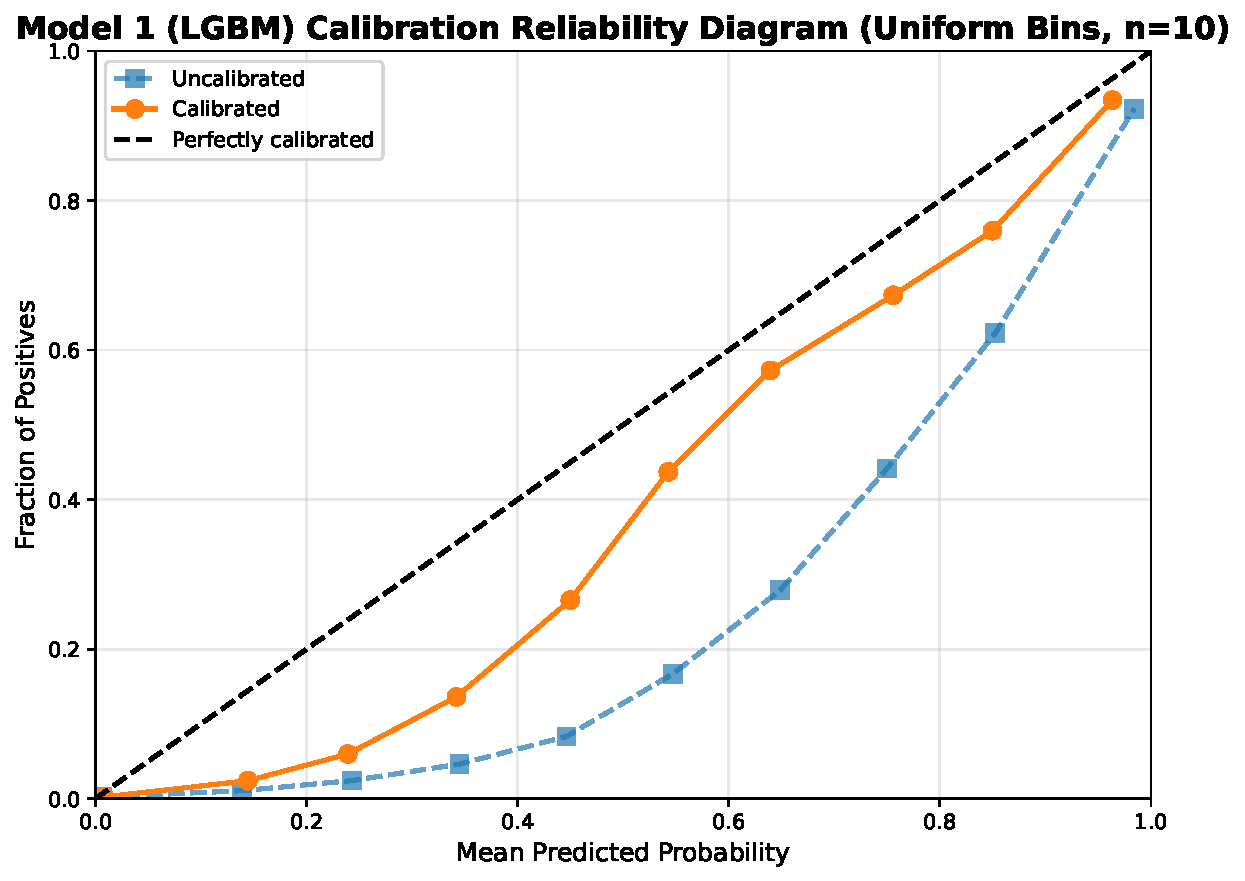
\includegraphics[width=\textwidth]{../outputs/south_america/results/model1_lgbm/calibration_reliability.pdf}
    \caption{South America: LightGBM}
  \end{subfigure}\hfill
  \begin{subfigure}[t]{0.48\textwidth}
    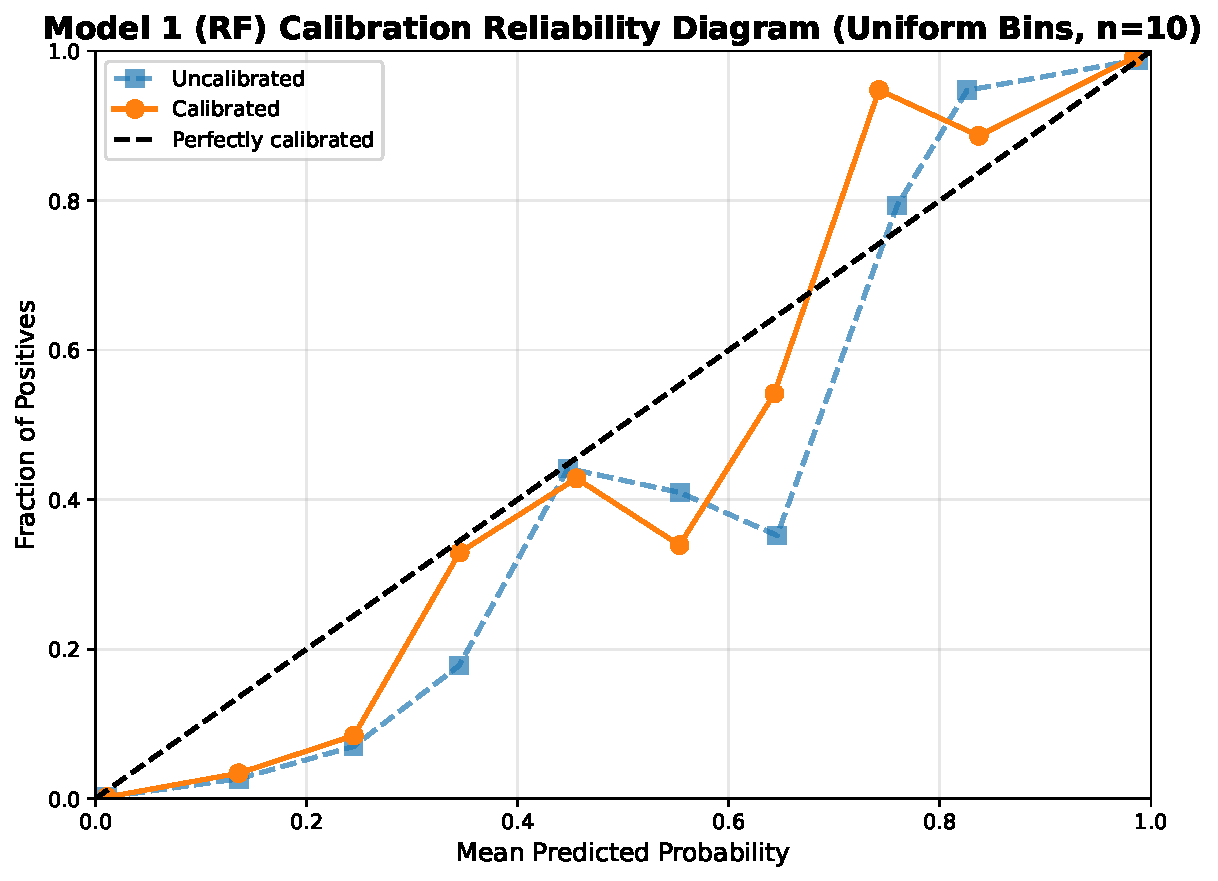
\includegraphics[width=\textwidth]{../outputs/south_america/results/model1_rf/calibration_reliability.pdf}
    \caption{South America: Random Forest}
  \end{subfigure}

  \vspace{0.8em}
  \begin{subfigure}[t]{0.48\textwidth}
    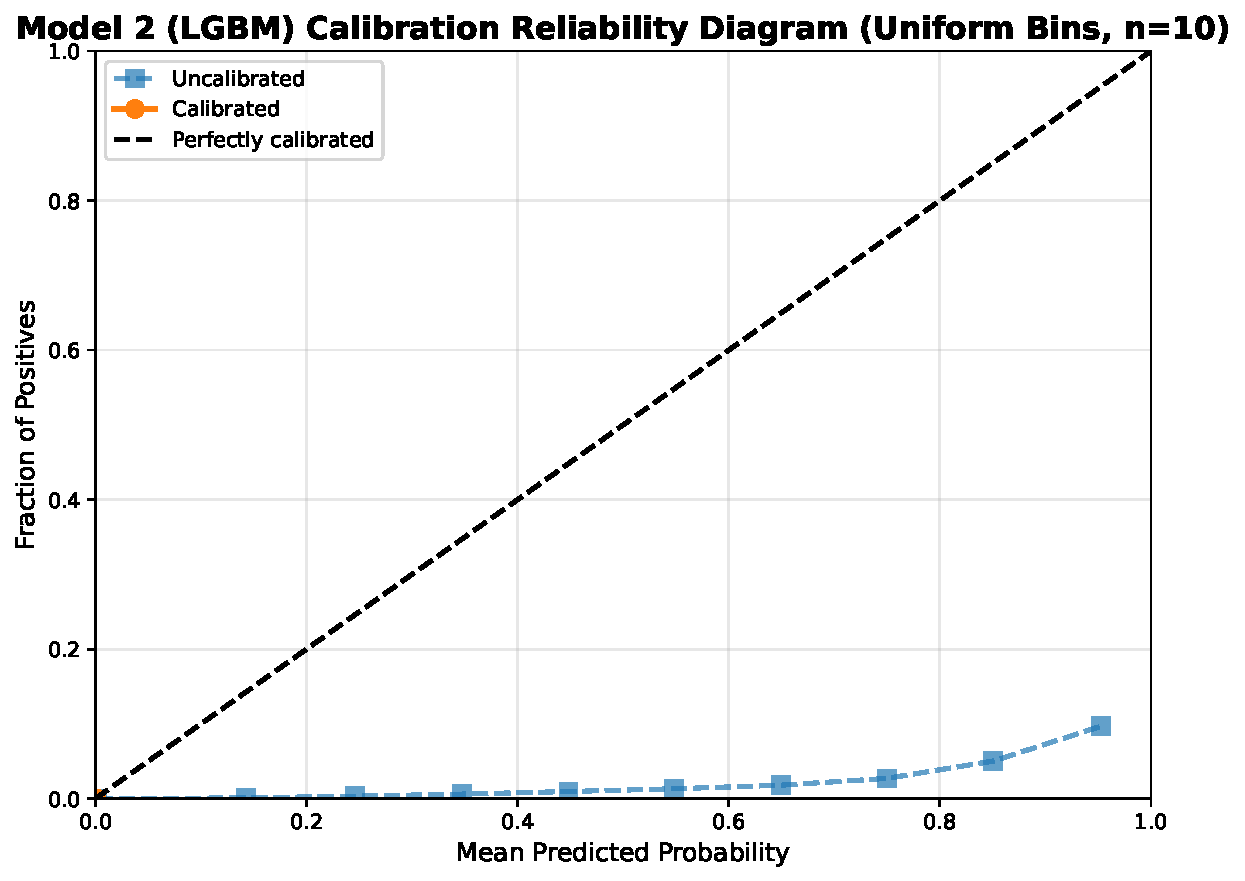
\includegraphics[width=\textwidth]{../outputs/usa/results/model2_lgbm/calibration_reliability.pdf}
    \caption{United States: LightGBM}
  \end{subfigure}\hfill
  \begin{subfigure}[t]{0.48\textwidth}
    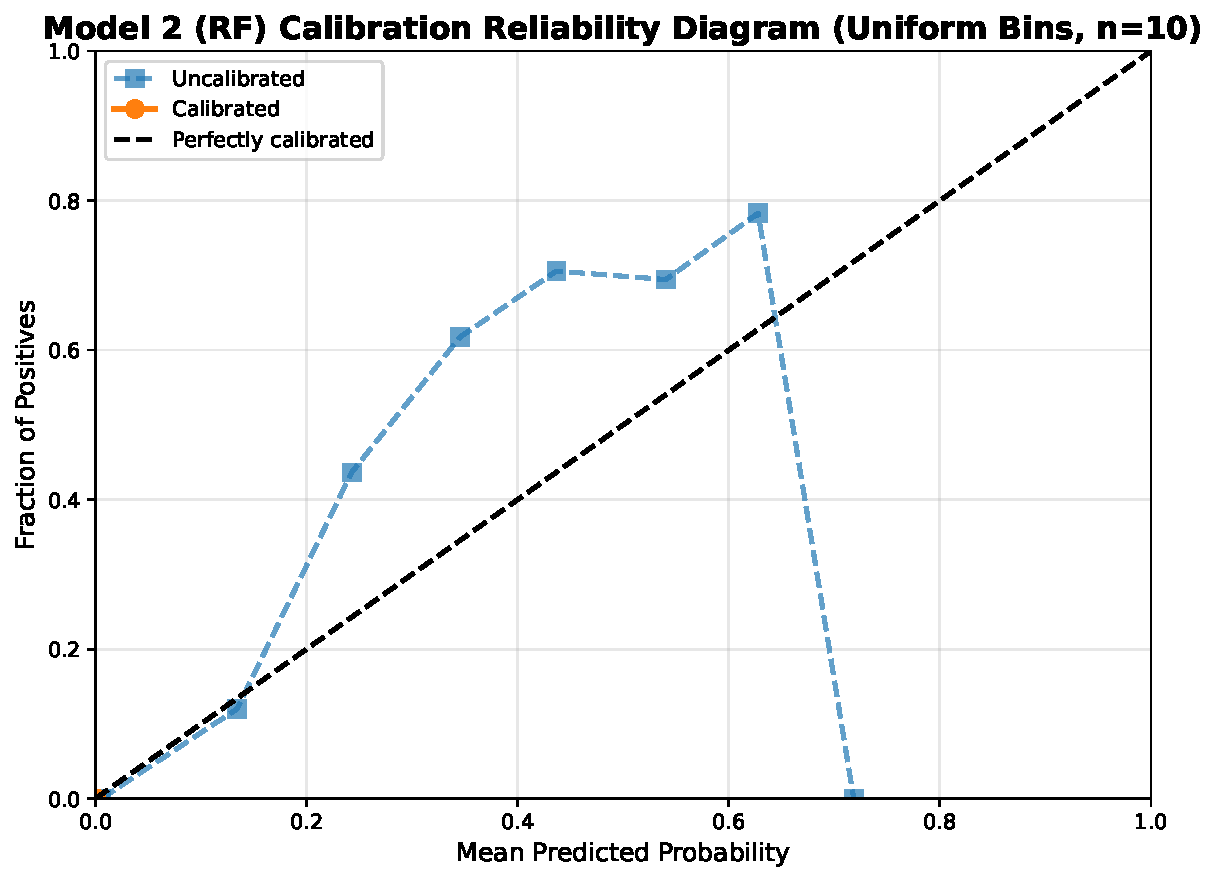
\includegraphics[width=\textwidth]{../outputs/usa/results/model2_rf/calibration_reliability.pdf}
    \caption{United States: Random Forest}
  \end{subfigure}

  \vspace{0.8em}
  \begin{subfigure}[t]{0.48\textwidth}
    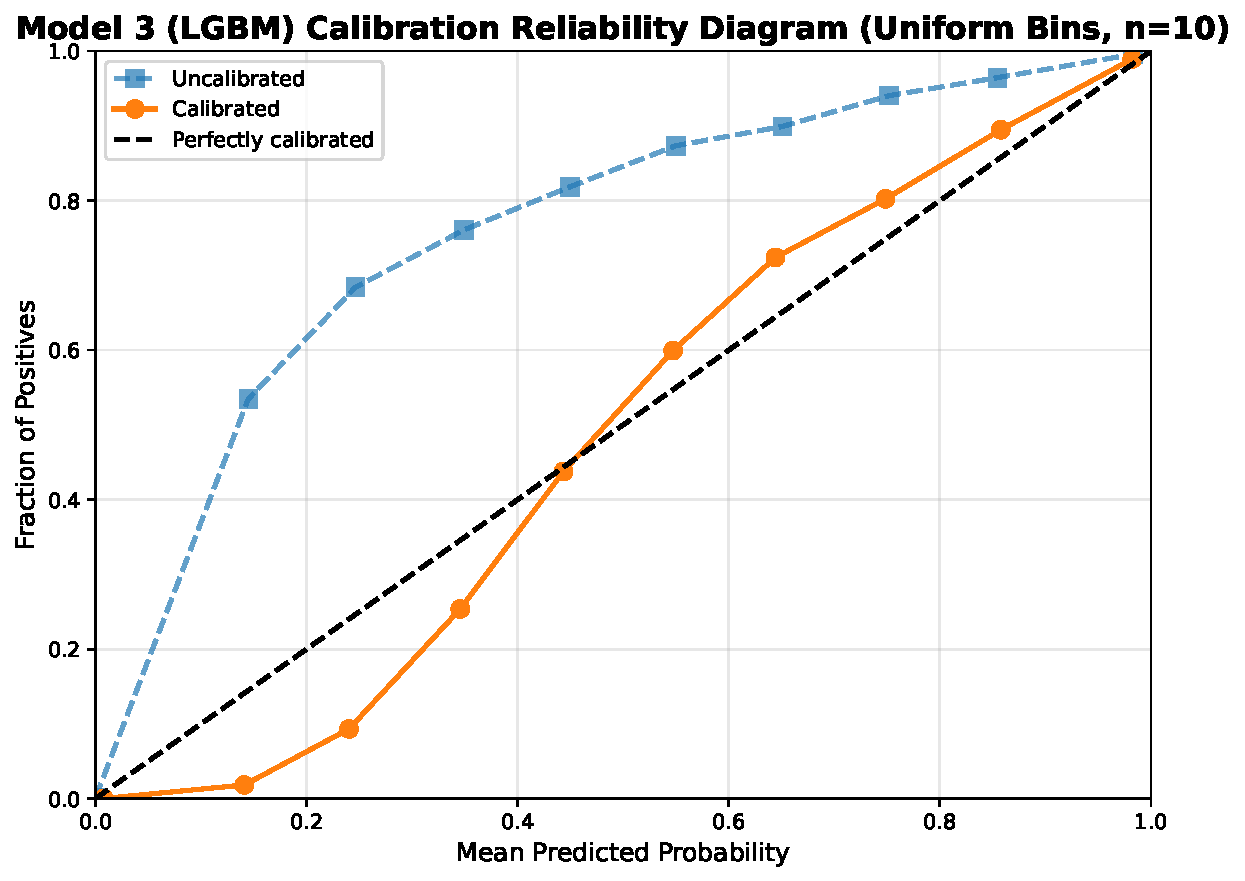
\includegraphics[width=\textwidth]{../outputs/se_asia/results/model3_lgbm/calibration_reliability.pdf}
    \caption{Southeast Asia: LightGBM}
  \end{subfigure}\hfill
  \begin{subfigure}[t]{0.48\textwidth}
    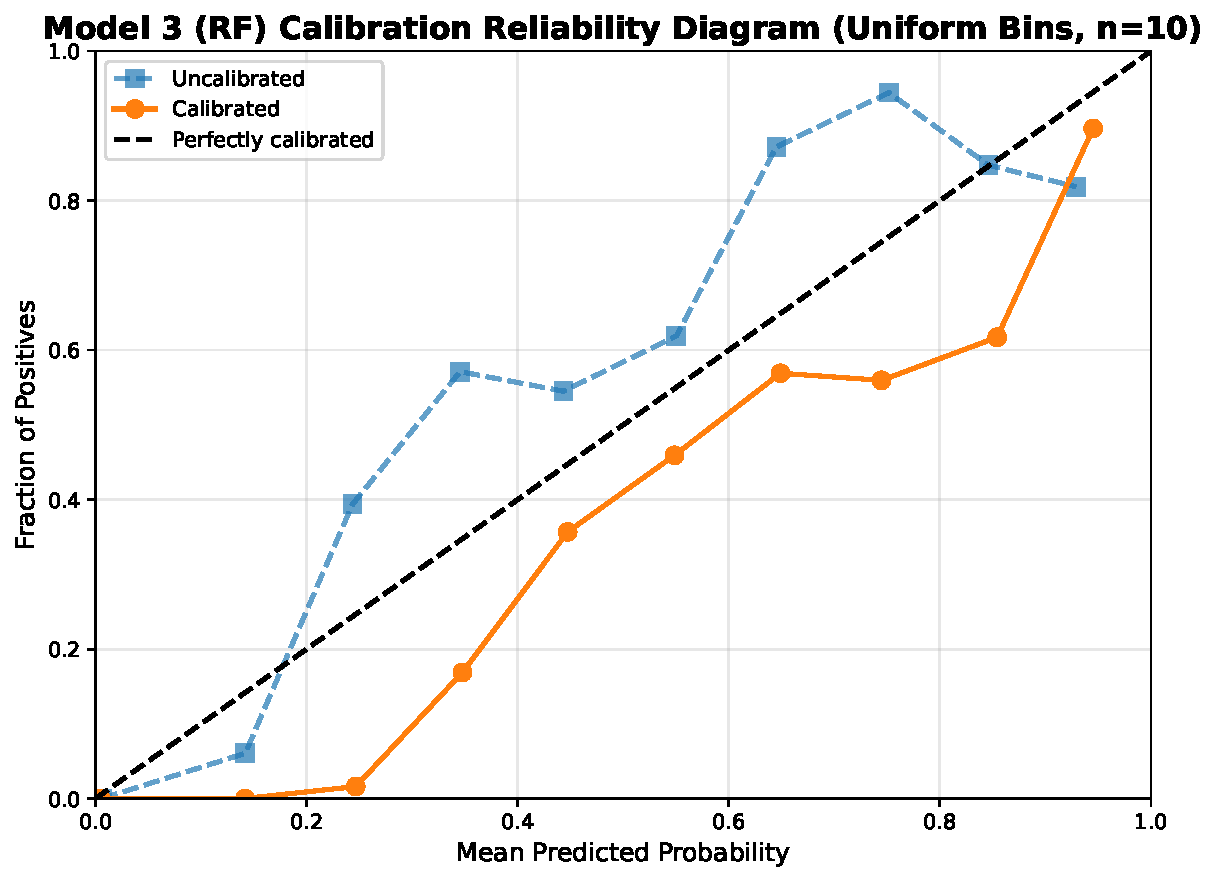
\includegraphics[width=\textwidth]{../outputs/se_asia/results/model3_rf/calibration_reliability.pdf}
    \caption{Southeast Asia: Random Forest}
  \end{subfigure}

  \caption{Reliability diagrams for all six model variants (before and after Platt
  scaling). Each bar shows the observed positive rate within the corresponding
  predicted-probability bin; perfect calibration is the $45^{\circ}$ diagonal.}
  \label{fig:reliability}
\end{figure}

\subsection{Cross-Continental Transfer Detail}
\label{app:transfer}

Cross-continental transfer is evaluated across all three continental pairs using the
73-feature set common to all regions. Each production model is serialised after
training on its home region (2001--2019) and scored on each other region's test
panel (2017--2019) without any retraining. Table~\ref{tab:transfer_full} reports ROC-AUC for all twelve direction--algorithm
combinations. ROC-AUC is used here because it is invariant to base-rate differences
across regions (unlike PR-AUC, which is strongly influenced by the positive rate of
the target region and would conflate transfer performance with base-rate shifts);
it is therefore the appropriate metric for comparing cross-regional discrimination.

\begin{table}[H]
\centering
\caption{Cross-continental transfer ROC-AUC (all directions). Test years 2017--2019.
Random-classifier baseline = 0.500. Values below 0.500 indicate the model has
learned patterns that are anti-correlated with designation in the target region.}
\label{tab:transfer_full}
\small
\begin{tabular}{llcc}
\toprule
\textbf{Direction} & \textbf{Algorithm} & \textbf{ROC-AUC} & \textbf{Interpretation} \\
\midrule
SA $\to$ USA         & LGBM & 0.517 & near-random \\
USA $\to$ SA         & LGBM & 0.518 & near-random \\
SA $\to$ SE Asia     & LGBM & 0.521 & near-random \\
USA $\to$ SE Asia    & LGBM & 0.617 & moderate transfer \\
SE Asia $\to$ SA     & LGBM & 0.381 & below random \\
SE Asia $\to$ USA    & LGBM & 0.238 & strongly below random \\
\midrule
SA $\to$ USA         & RF   & 0.301 & below random \\
USA $\to$ SA         & RF   & 0.531 & near-random \\
SA $\to$ SE Asia     & RF   & 0.720 & substantial transfer \\
USA $\to$ SE Asia    & RF   & 0.614 & moderate transfer \\
SE Asia $\to$ SA     & RF   & 0.598 & moderate transfer \\
SE Asia $\to$ USA    & RF   & 0.713 & substantial transfer \\
\bottomrule
\end{tabular}
\end{table}

The LGBM results are internally consistent: SA--USA LGBM transfer is near-random in
both directions, while transfers involving SE Asia diverge; the SE Asia model
applies anti-predictively to the Americas (ROC-AUC well below 0.5), reflecting that
the feature combinations most predictive of PA designation in SE Asia (forested
upland areas in Borneo and the Mekong region) are not where designation happens in
the Americas. The RF results show a different pattern: SA$\to$SE Asia and SE
Asia$\to$USA both achieve ROC-AUC $\approx 0.71$--$0.72$, suggesting that the
bagged ensemble has learned more robust ecological baselines that partially transfer,
whereas the gradient-boosted LGBM has overfit to institutional patterns specific to
each region. The SA$\to$USA RF (0.301) replicates the below-random phenomenon seen
for LGBM SE Asia transfers, pointing to genuine anti-correlation between SA
high-designation features and US high-designation pixels.

Taken together, the results confirm that LGBM-based transition-risk scores require
region-specific calibration, while also suggesting that future generalisation efforts
may benefit from ensemble or bagging architectures that suppress institutional
overfitting. The RF/LGBM contrast is substantively important and is discussed in
Section~\ref{sec:disc_transfer}.

\subsection{Backtesting Results}
\label{app:backtest}

Walk-forward backtests at origins $T \in \{2009, 2011\}$ verify that deployment-style
inference generalises to out-of-sample designation events. SA LightGBM Precision@1\%
at $T=2009$: approximately 0.48; at $T=2011$: approximately 0.51 (stable relative to
the test-period 0.532). USA Precision@1\% is lower ($\approx 0.010$--$0.015$) and
more variable, consistent with the near-zero test-set Precision@1\% (0.033) driven
by the extremely low US positive rate.
%TODO: NEEDS COMPUTATION: verify and update backtest precision values from forward_backtest_precision_over_time figures; add a summary table with PR-AUC per origin.

\paragraph{False positive spatial patterns.}
Figures~\ref{fig:fp_sa_2017}--\ref{fig:fp_usa_2017} map the spatial distribution of
false positives for South America and the United States using the production
test-set model (training period 2001--2019, evaluated on 2017--2019 test pixels):
pixels that fall within the top-1\% predicted risk zone but were not designated
within the subsequent five-year window. In South America, false positives concentrate
along the southern and eastern Amazon frontier (Mato Grosso, Par\'a) and in Andean
foothills, the same zones where genuine designations are clustered, suggesting that
many false positives are temporally rather than geographically misplaced: the model
correctly identifies active designation frontiers but the specific parcels flagged were
designated slightly before or after the evaluation window. In the United States, false
positives are concentrated in arid BLM landscapes of the West, reflecting that the
model assigns high risk to a large contiguous landscape zone, only a fraction of which
receives formal designation in any five-year period.

\begin{figure}[H]
  \centering
  \begin{subfigure}[t]{0.48\textwidth}
    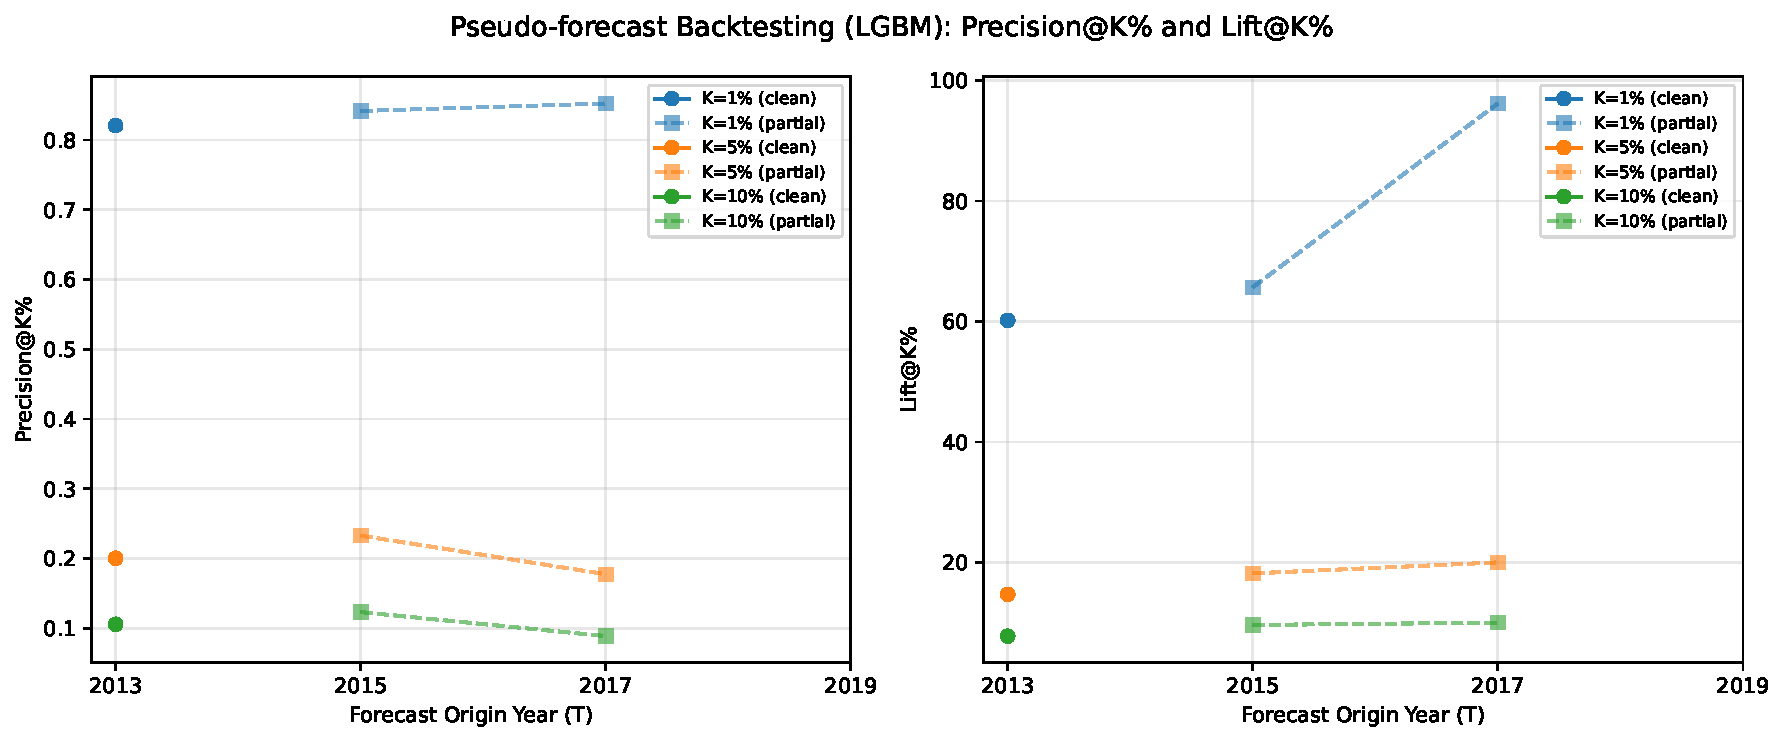
\includegraphics[width=\textwidth]{../outputs/south_america/results/forward/lgbm/forward_backtest_precision_over_time.pdf}
    \caption{South America: LightGBM}
  \end{subfigure}\hfill
  \begin{subfigure}[t]{0.48\textwidth}
    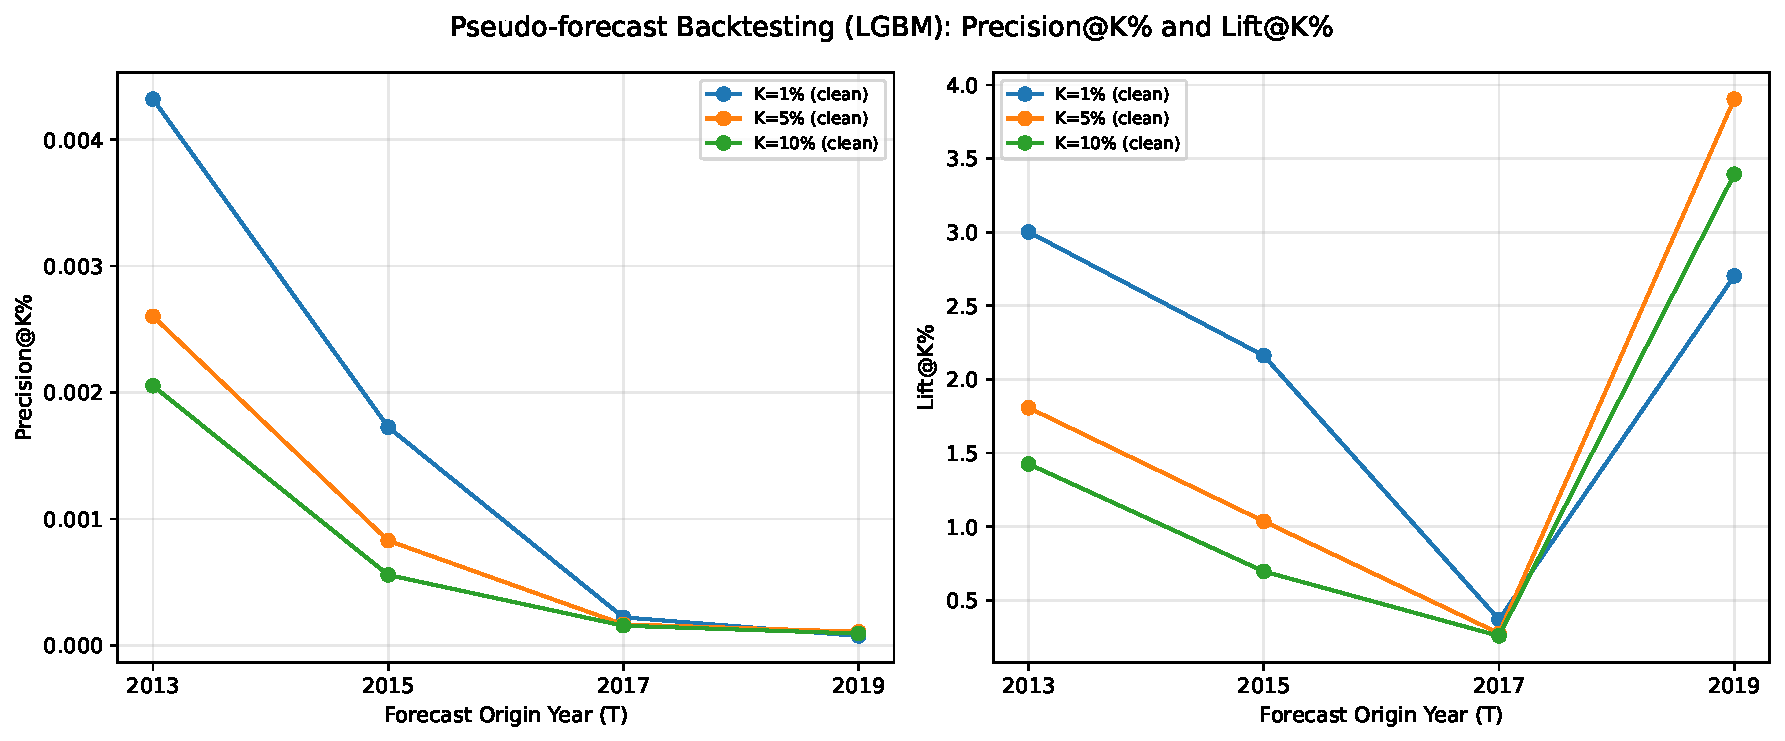
\includegraphics[width=\textwidth]{../outputs/usa/results/forward/lgbm/forward_backtest_precision_over_time.pdf}
    \caption{United States: LightGBM}
  \end{subfigure}

  \vspace{0.8em}
  \begin{subfigure}[t]{0.48\textwidth}
    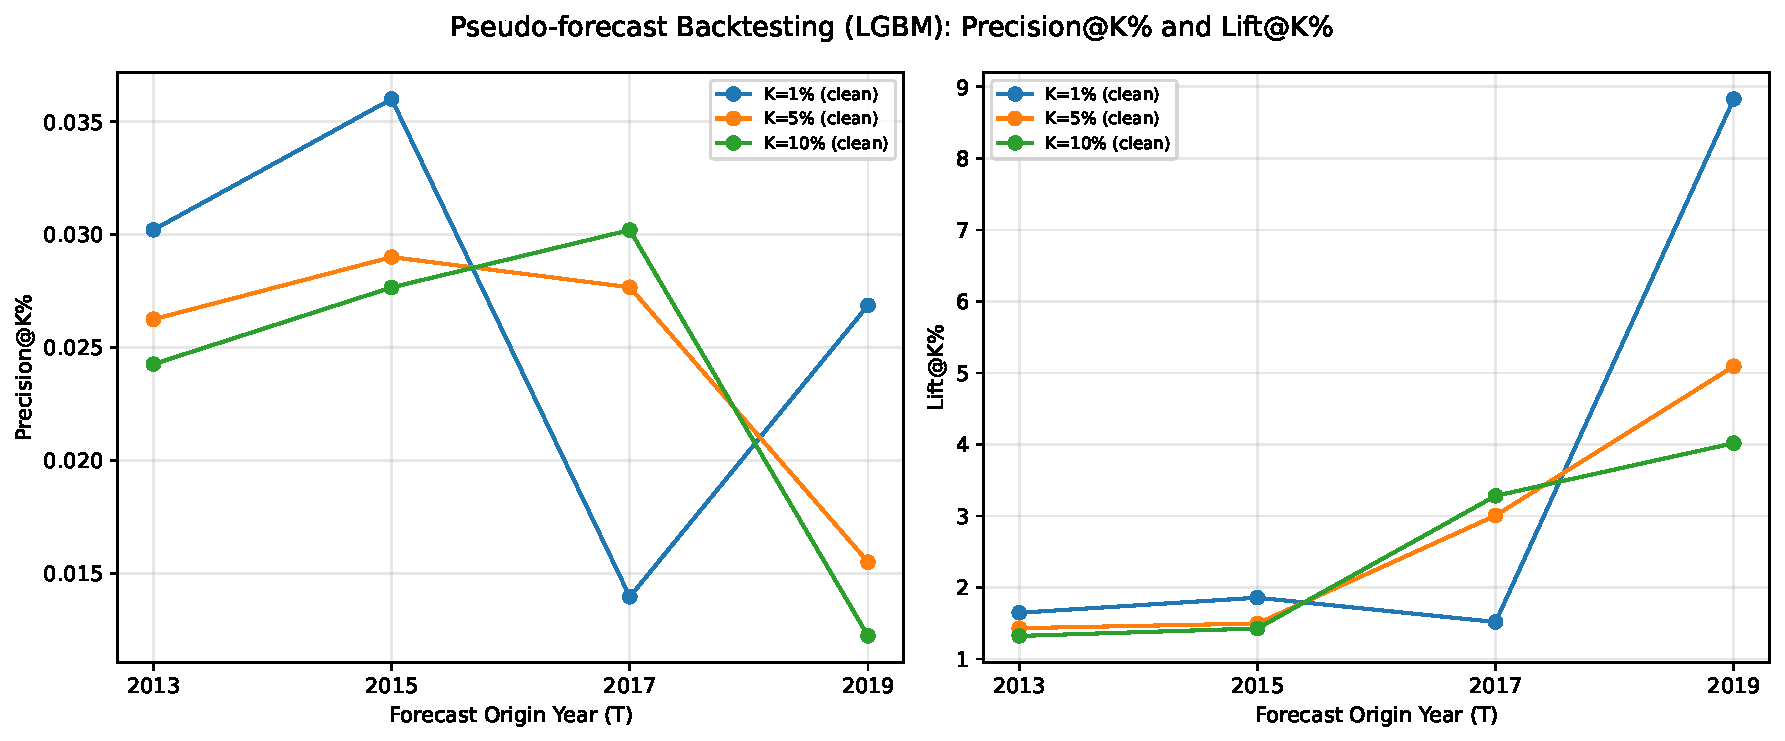
\includegraphics[width=\textwidth]{../outputs/se_asia/results/forward/lgbm/forward_backtest_precision_over_time.pdf}
    \caption{Southeast Asia: LightGBM}
  \end{subfigure}

  \caption{Backtesting precision@1\% over time for walk-forward forecasts at origins
  $T \in \{2009, 2011\}$. Each line shows the precision of the top-1\% of unprotected
  pixels scored in year $T$ (i.e.\ the $\approx 1\%$ highest-ranked pixels among all
  pixels eligible in that origin year), evaluated against realised 5-year designation
  outcomes in years $T{+}1$ through $T{+}5$.}
  \label{fig:backtest}
\end{figure}

\begin{figure}[H]
  \centering
  \begin{subfigure}[t]{0.48\textwidth}
    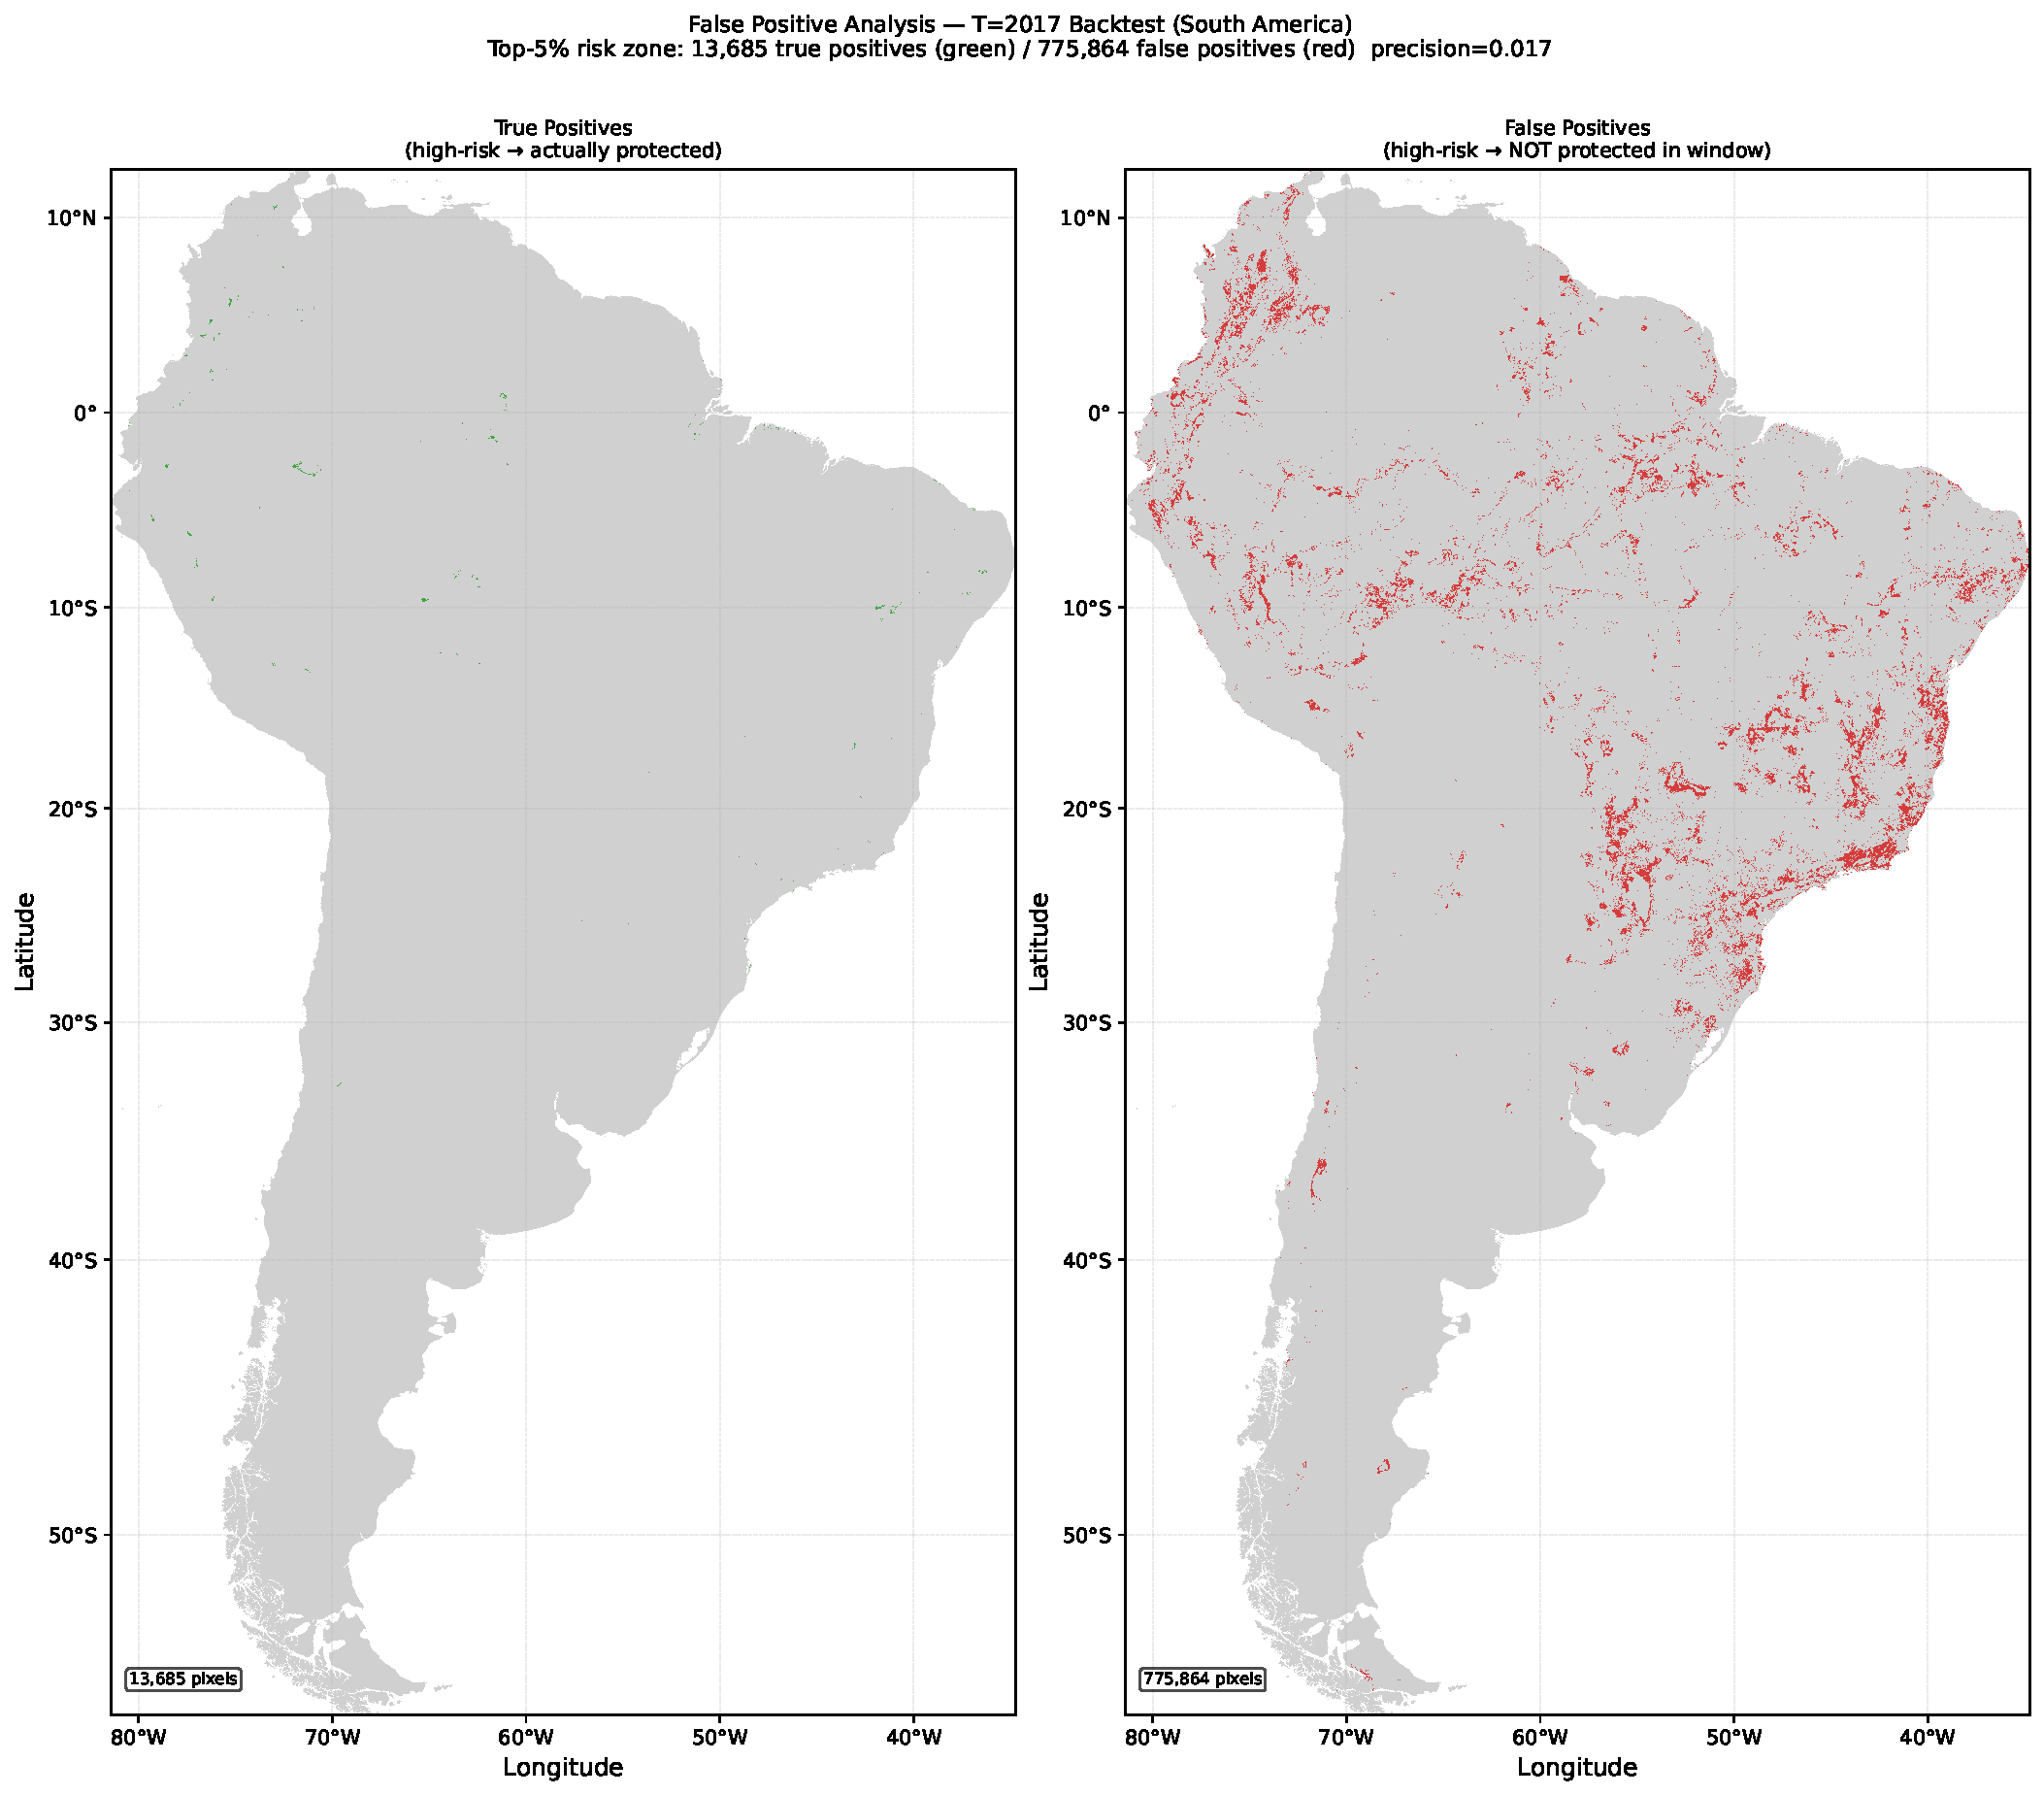
\includegraphics[width=\textwidth]{../outputs/south_america/results/forward/lgbm/forward_backtest_T2017_false_positives.pdf}
    \caption{South America: false positives at $T=2017$}
    \label{fig:fp_sa_2017}
  \end{subfigure}\hfill
  \begin{subfigure}[t]{0.48\textwidth}
    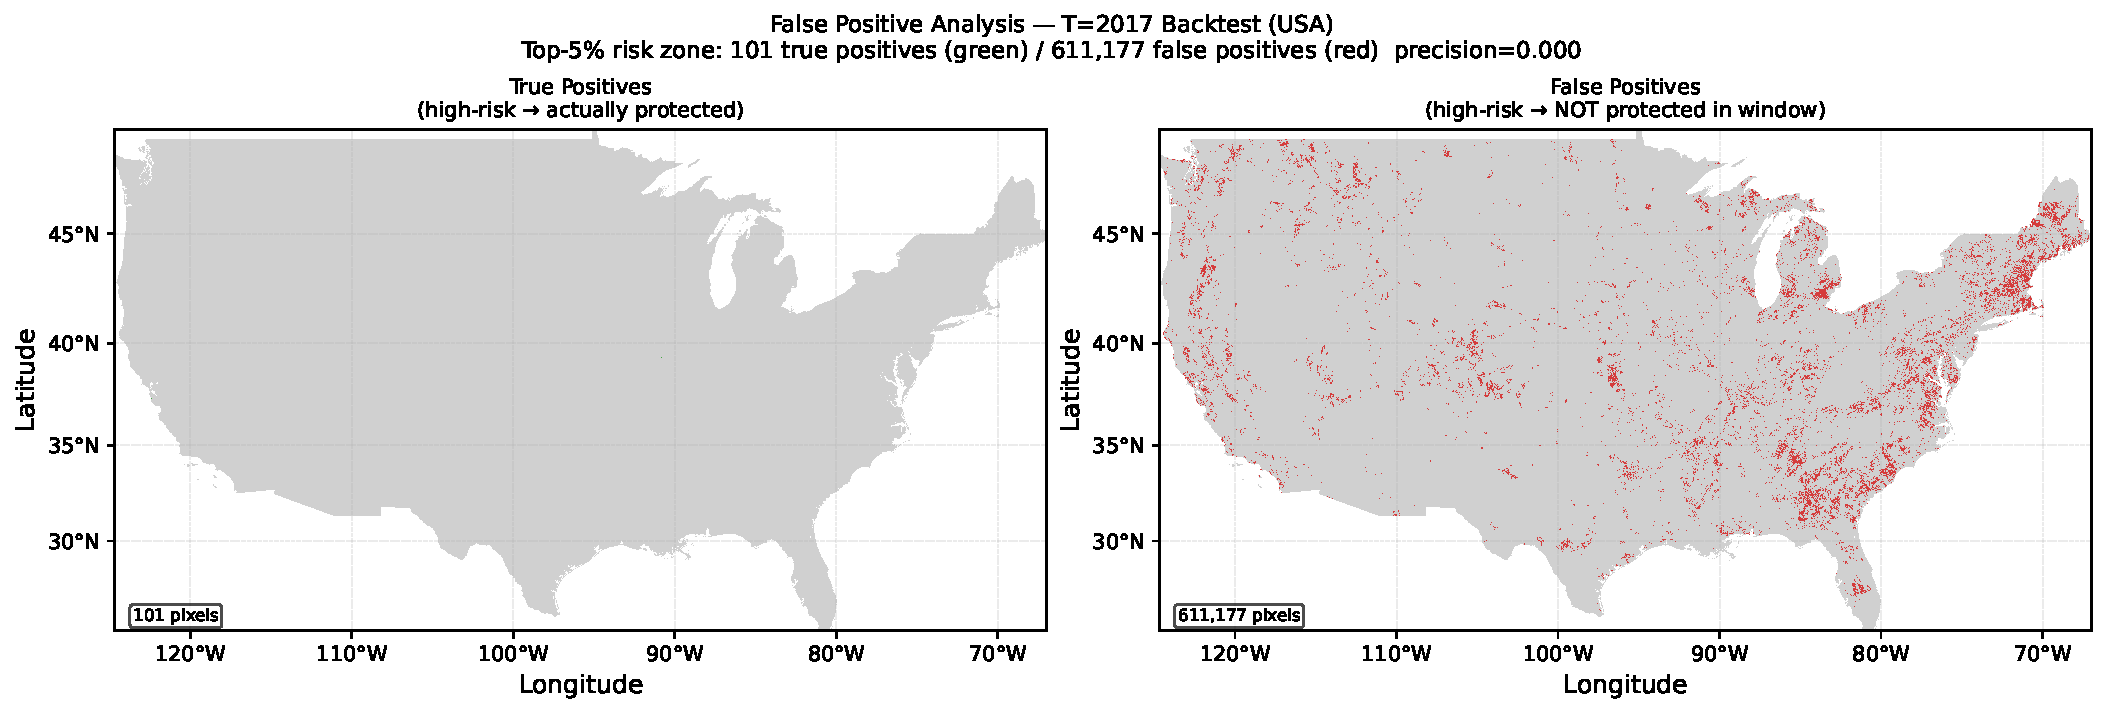
\includegraphics[width=\textwidth]{../outputs/usa/results/forward/lgbm/forward_backtest_T2017_false_positives.pdf}
    \caption{United States: false positives at $T=2017$}
    \label{fig:fp_usa_2017}
  \end{subfigure}
  \caption{Spatial distribution of false positives at backtest origin $T=2017$:
  pixels in the top-1\% predicted risk zone that were not designated within the
  subsequent five-year window. Clustering of false positives in known designation
  frontiers (Amazon arc, BLM arid West) suggests temporal rather than geographic
  misclassification for most cases.}
  \label{fig:fp_backtest}
\end{figure}

\section{Feature Dictionary}
\label{app:features}

Table~\ref{tab:features} lists the full feature set used in the South America, USA,
and Southeast Asia models. All three regions share the same 73-feature schema,
derived from the predictor groups in Table~\ref{tab:data} via multi-scale spatial
smoothing ($4\times4$, $16\times16$, $64\times64$ km), Euclidean distance transforms,
and temporal lags.

\footnotesize
\begin{longtable}{%
  >{\raggedright\arraybackslash}p{0.30\linewidth}%
  >{\raggedright\arraybackslash}p{0.12\linewidth}%
  >{\raggedright\arraybackslash}p{0.52\linewidth}%
}
\caption{Complete feature dictionary (73 features). All three continental models
share this schema, derived via multi-scale spatial smoothing
($4\times4$, $16\times16$, $64\times64$~km for all smoothed variables),
Euclidean distance transforms, and temporal lags.
\textit{Static} = time-invariant; \textit{Dynamic} = updated annually.}
\label{tab:features} \\
\toprule
\textbf{Feature name} & \textbf{Type} & \textbf{Description} \\
\midrule
\endfirsthead
\multicolumn{3}{l}{\small\textit{Continued from previous page}} \\
\toprule
\textbf{Feature name} & \textbf{Type} & \textbf{Description} \\
\midrule
\endhead
\midrule
\multicolumn{3}{r}{\small\textit{Continued on next page}} \\
\endfoot
\bottomrule
\endlastfoot
%% ---- Terrain ---------------------------------------------------------------
\multicolumn{3}{l}{\textit{Terrain (CGIAR SRTM V4; static)}} \\
\midrule
\texttt{elevation\_b1}          & Static  & Elevation (m) \\
\texttt{elevation\_b1\_smooth4} & Static  & Elevation averaged over $4\times4$ km window \\
\texttt{elevation\_b1\_smooth16}& Static  & Elevation averaged over $16\times16$ km window \\
\texttt{elevation\_b1\_smooth64}& Static  & Elevation averaged over $64\times64$ km window \\
\texttt{elevation\_b2}          & Static  & Terrain slope (degrees, derived from SRTM) \\
\texttt{elevation\_b2\_smooth4} & Static  & Slope averaged over $4\times4$ km window \\
\texttt{elevation\_b2\_smooth16}& Static  & Slope averaged over $16\times16$ km window \\
\texttt{elevation\_b2\_smooth64}& Static  & Slope averaged over $64\times64$ km window \\
\midrule
%% ---- Climate ---------------------------------------------------------------
\multicolumn{3}{l}{\textit{Climate — WorldClim V1 bioclimatic normals (1950--2000; static)}} \\
\midrule
\texttt{WorldClim\_b1}  & Static & Annual mean temperature \\
\texttt{WorldClim\_b2}  & Static & Mean diurnal temperature range \\
\texttt{WorldClim\_b3}  & Static & Isothermality (mean diurnal range / temperature annual range) \\
\texttt{WorldClim\_b4}  & Static & Temperature seasonality (standard deviation) \\
\texttt{WorldClim\_b5}  & Static & Maximum temperature of warmest month \\
\texttt{WorldClim\_b6}  & Static & Minimum temperature of coldest month \\
\texttt{WorldClim\_b7}  & Static & Temperature annual range \\
\texttt{WorldClim\_b8}  & Static & Mean temperature of wettest quarter \\
\texttt{WorldClim\_b9}  & Static & Mean temperature of driest quarter \\
\texttt{WorldClim\_b10} & Static & Mean temperature of warmest quarter \\
\texttt{WorldClim\_b11} & Static & Mean temperature of coldest quarter \\
\texttt{WorldClim\_b12} & Static & Annual precipitation (mm) \\
\texttt{WorldClim\_b13} & Static & Precipitation of wettest month (mm) \\
\texttt{WorldClim\_b14} & Static & Precipitation of driest month (mm) \\
\texttt{WorldClim\_b15} & Static & Precipitation seasonality (coefficient of variation) \\
\texttt{WorldClim\_b16} & Static & Precipitation of wettest quarter (mm) \\
\texttt{WorldClim\_b17} & Static & Precipitation of driest quarter (mm) \\
\texttt{WorldClim\_b18} & Static & Precipitation of warmest quarter (mm) \\
\texttt{WorldClim\_b19} & Static & Precipitation of coldest quarter (mm) \\
\midrule
%% ---- Biodiversity ----------------------------------------------------------
\multicolumn{3}{l}{\textit{Biodiversity priority — Global Safety Net layers (static)}} \\
\midrule
\texttt{GSN\_b1}          & Static & Climate stabilisation area indicator (binary, GSN) \\
\texttt{GSN\_b1\_smooth16}& Static & Climate stabilisation area at $16\times16$ km \\
\texttt{GSN\_b1\_smooth64}& Static & Climate stabilisation area at $64\times64$ km \\
\texttt{GSN\_b2}          & Static & High-biodiversity area indicator (binary, GSN) \\
\texttt{GSN\_b2\_smooth16}& Static & High-biodiversity area at $16\times16$ km \\
\texttt{GSN\_b2\_smooth64}& Static & High-biodiversity area at $64\times64$ km \\
\texttt{GSN\_b3}          & Static & Intact wilderness area indicator (binary, GSN) \\
\texttt{GSN\_b3\_smooth16}& Static & Intact wilderness area at $16\times16$ km \\
\texttt{GSN\_b3\_smooth64}& Static & Intact wilderness area at $64\times64$ km \\
\texttt{GSN\_b4}          & Static & Potential wildlife corridor indicator (binary, GSN) \\
\texttt{GSN\_b4\_smooth16}& Static & Wildlife corridor area at $16\times16$ km \\
\texttt{GSN\_b4\_smooth64}& Static & Wildlife corridor area at $64\times64$ km \\
\texttt{GSN\_b5}          & Static & Terrestrial ecoregion code (categorical, WWF via GSN; integer-encoded, designated as categorical to LightGBM so the tree learner optimises over all partition splits rather than imposing ordinal ordering) \\
\texttt{GSN\_b5\_smooth16}& Static & Ecoregion code majority at $16\times16$ km \\
\texttt{GSN\_b5\_smooth64}& Static & Ecoregion code majority at $64\times64$ km \\
\midrule
%% ---- Infrastructure --------------------------------------------------------
\multicolumn{3}{l}{\textit{Infrastructure and distance (static)}} \\
\midrule
\texttt{dist\_road}       & Static & Euclidean distance to nearest major road (m, GRIP) \\
\texttt{dist\_powerplant} & Static & Euclidean distance to nearest power plant (m, WRI GPPD) \\
\texttt{dist\_oil\_gas}   & Static & Euclidean distance to nearest oil/gas infrastructure (m) \\
\texttt{dist\_indigenous} & Static & Euclidean distance to nearest indigenous/community land (m, LandMark) \\
\texttt{powerplants\_b2}  & Static & Dominant fuel type of power plants in pixel (categorical, WRI GPPD) \\
\midrule
%% ---- Vegetation / land change ----------------------------------------------
\multicolumn{3}{l}{\textit{Vegetation and land cover (dynamic)}} \\
\midrule
\texttt{NDVI}             & Dynamic & Annual median NDVI (MODIS MOD13Q1) \\
\texttt{NDVI\_smooth16}   & Dynamic & NDVI averaged over $16\times16$ km window \\
\texttt{NDVI\_smooth64}   & Dynamic & NDVI averaged over $64\times64$ km window \\
\texttt{landcover}        & Dynamic & Annual dominant land-cover class (MODIS MCD12Q1) \\
\texttt{deforestation\_b1}& Dynamic & Annual remaining tree canopy cover (\%, Hansen GFC) \\
\texttt{deforestation\_b1\_smooth16} & Dynamic & Tree canopy cover at $16\times16$ km \\
\texttt{deforestation\_b1\_smooth64} & Dynamic & Tree canopy cover at $64\times64$ km \\
\texttt{deforestation\_b2}& Dynamic & Annual forest-loss indicator (binary, Hansen GFC) \\
\texttt{deforestation\_b3}& Dynamic & Cumulative forest loss since 2000 (binary, Hansen GFC) \\
\texttt{wildfire\_b1}     & Dynamic & Annual burned sub-pixel count within the 1-km cell (MODIS MCD64A1; count of 500-m cells with a detected burn date $>0$) \\
\texttt{wildfire\_b1\_smooth16} & Dynamic & Burned area at $16\times16$ km \\
\texttt{wildfire\_b1\_smooth64} & Dynamic & Burned area at $64\times64$ km \\
\texttt{wildfire\_b2}     & Dynamic & Annual binary burned mask (MODIS MCD64A1) \\
\midrule
%% ---- Human activity --------------------------------------------------------
\multicolumn{3}{l}{\textit{Population and human activity (dynamic)}} \\
\midrule
\texttt{GPW}              & Dynamic & Population density (persons/km\textsuperscript{2}, GPW v4, forward-filled) \\
\texttt{GPW\_smooth16}    & Dynamic & Population density at $16\times16$ km \\
\texttt{GPW\_smooth64}    & Dynamic & Population density at $64\times64$ km \\
\texttt{HNTL}             & Dynamic & Night-time lights luminosity (DMSP/VIIRS harmonised) \\
\texttt{HNTL\_smooth16}   & Dynamic & Night-time lights at $16\times16$ km \\
\texttt{HNTL\_smooth64}   & Dynamic & Night-time lights at $64\times64$ km \\
\midrule
%% ---- Protection ------------------------------------------------------------
\multicolumn{3}{l}{\textit{Protection status and proximity (dynamic)}} \\
\midrule
\texttt{WDPA}             & Dynamic & Previous-year protected area status (binary, WDPA; always 0 for risk-set eligible pixels by construction, providing no leakage; at inference time the feature is set to 0 for all scored pixels) \\
\texttt{dist\_wdpa}       & Dynamic & Euclidean distance to nearest PA boundary (m), lagged 1 yr \\
\midrule
%% ---- Governance ------------------------------------------------------------
\multicolumn{3}{l}{\textit{Governance and policy (country-level; dynamic)}} \\
\midrule
\texttt{policy\_b1} & Dynamic & Executive ideology (DPI; $-1$=Left, $0$=Centre, $+1$=Right) \\
\texttt{policy\_b2} & Dynamic & V-Dem Liberal Democracy Index (0--1) \\
\texttt{policy\_b3} & Dynamic & WGI Government Effectiveness ($\approx{-2.5}$ to $+2.5$) \\
\texttt{policy\_b4} & Dynamic & WGI Rule of Law ($\approx{-2.5}$ to $+2.5$) \\
\midrule
%% ---- Economic --------------------------------------------------------------
\multicolumn{3}{l}{\textit{Economic value (dynamic)}} \\
\midrule
\texttt{economic\_value\_lag1} & Dynamic & Agricultural land value (USD/ha, FAO FAOSTAT), lagged 1 yr \\
\end{longtable}

\section{Regional Supplementary Results}
\label{app:supp_figures}

%TODO: NEEDS COMPUTATION: regenerate USA and SE Asia LOBO bar charts from
% corrected Euler results
% (spatial_cv_visualisation/bar_lobo_performance_lgbm.pdf for each region) and
% uncomment the figures below before final submission.
%
%\begin{figure}[H]
%\centering
%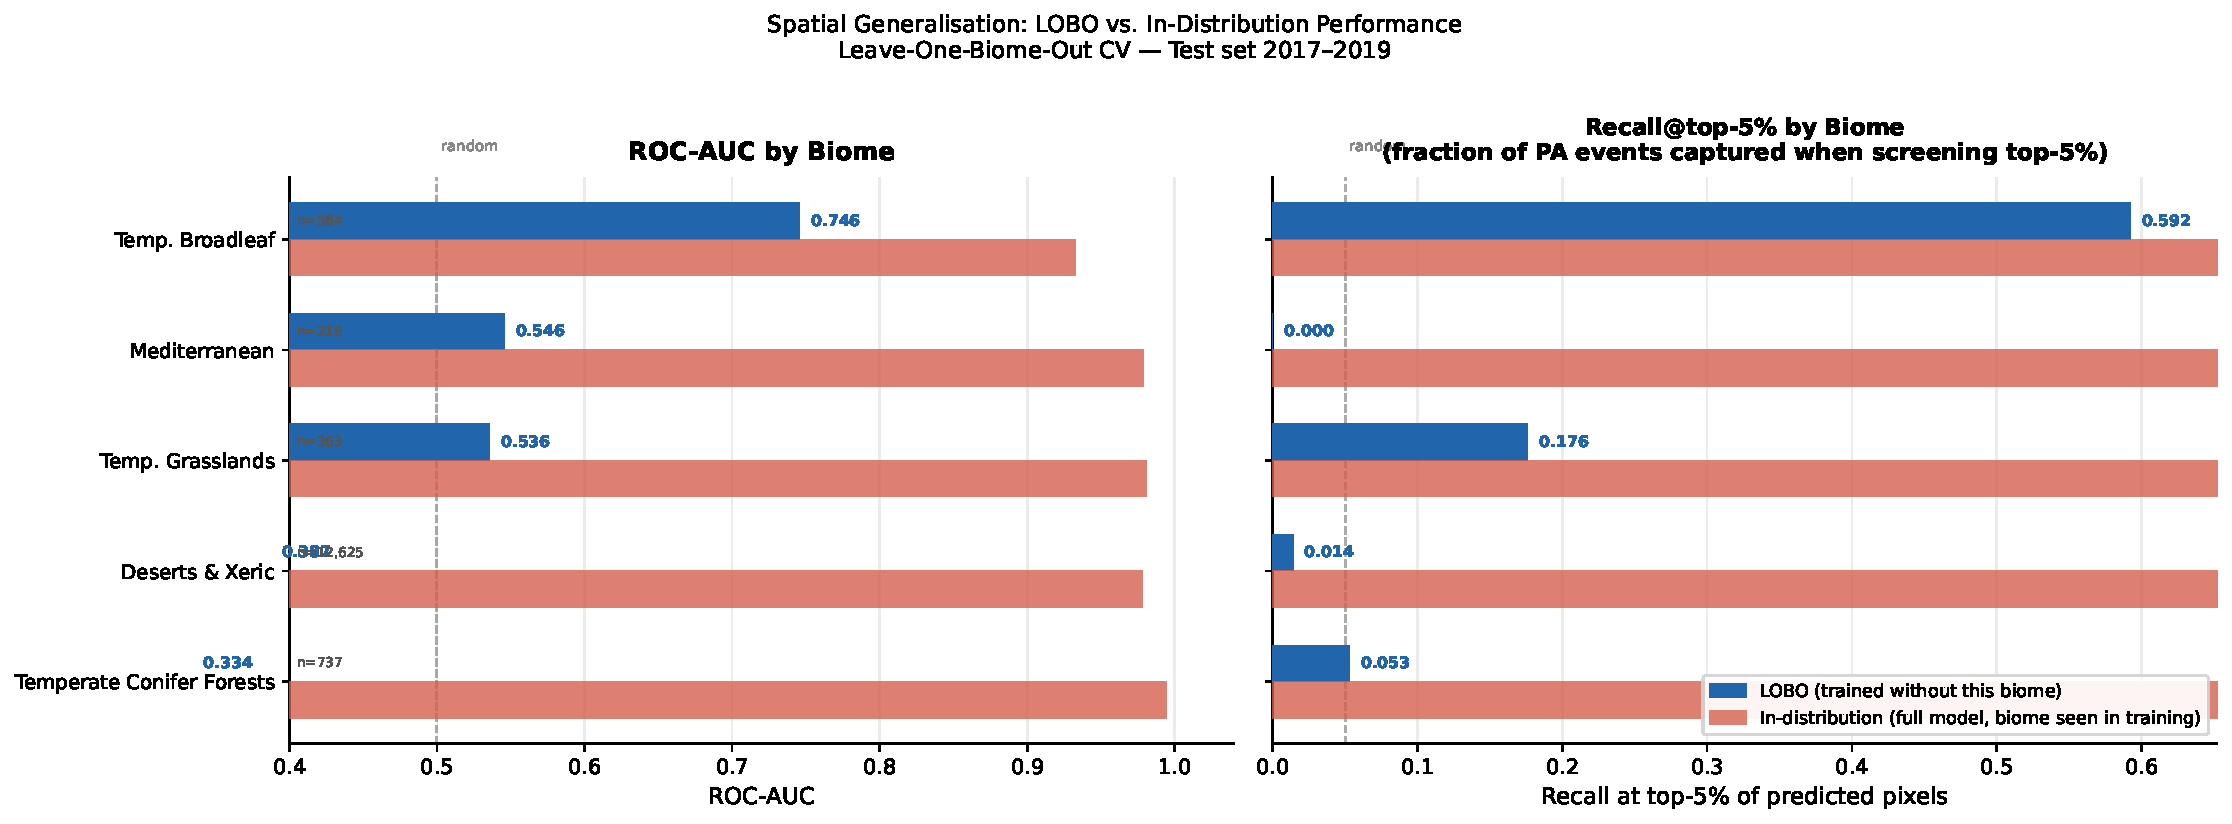
\includegraphics[width=\textwidth, keepaspectratio]{../outputs/usa/results/spatial_cv_visualisation/bar_lobo_performance_lgbm.pdf}
%\caption{Per-biome LOBO PR-AUC for the United States (LightGBM, test set 2017--2019).}
%\label{fig:lobo_usa}
%\end{figure}
%
%\begin{figure}[H]
%\centering
%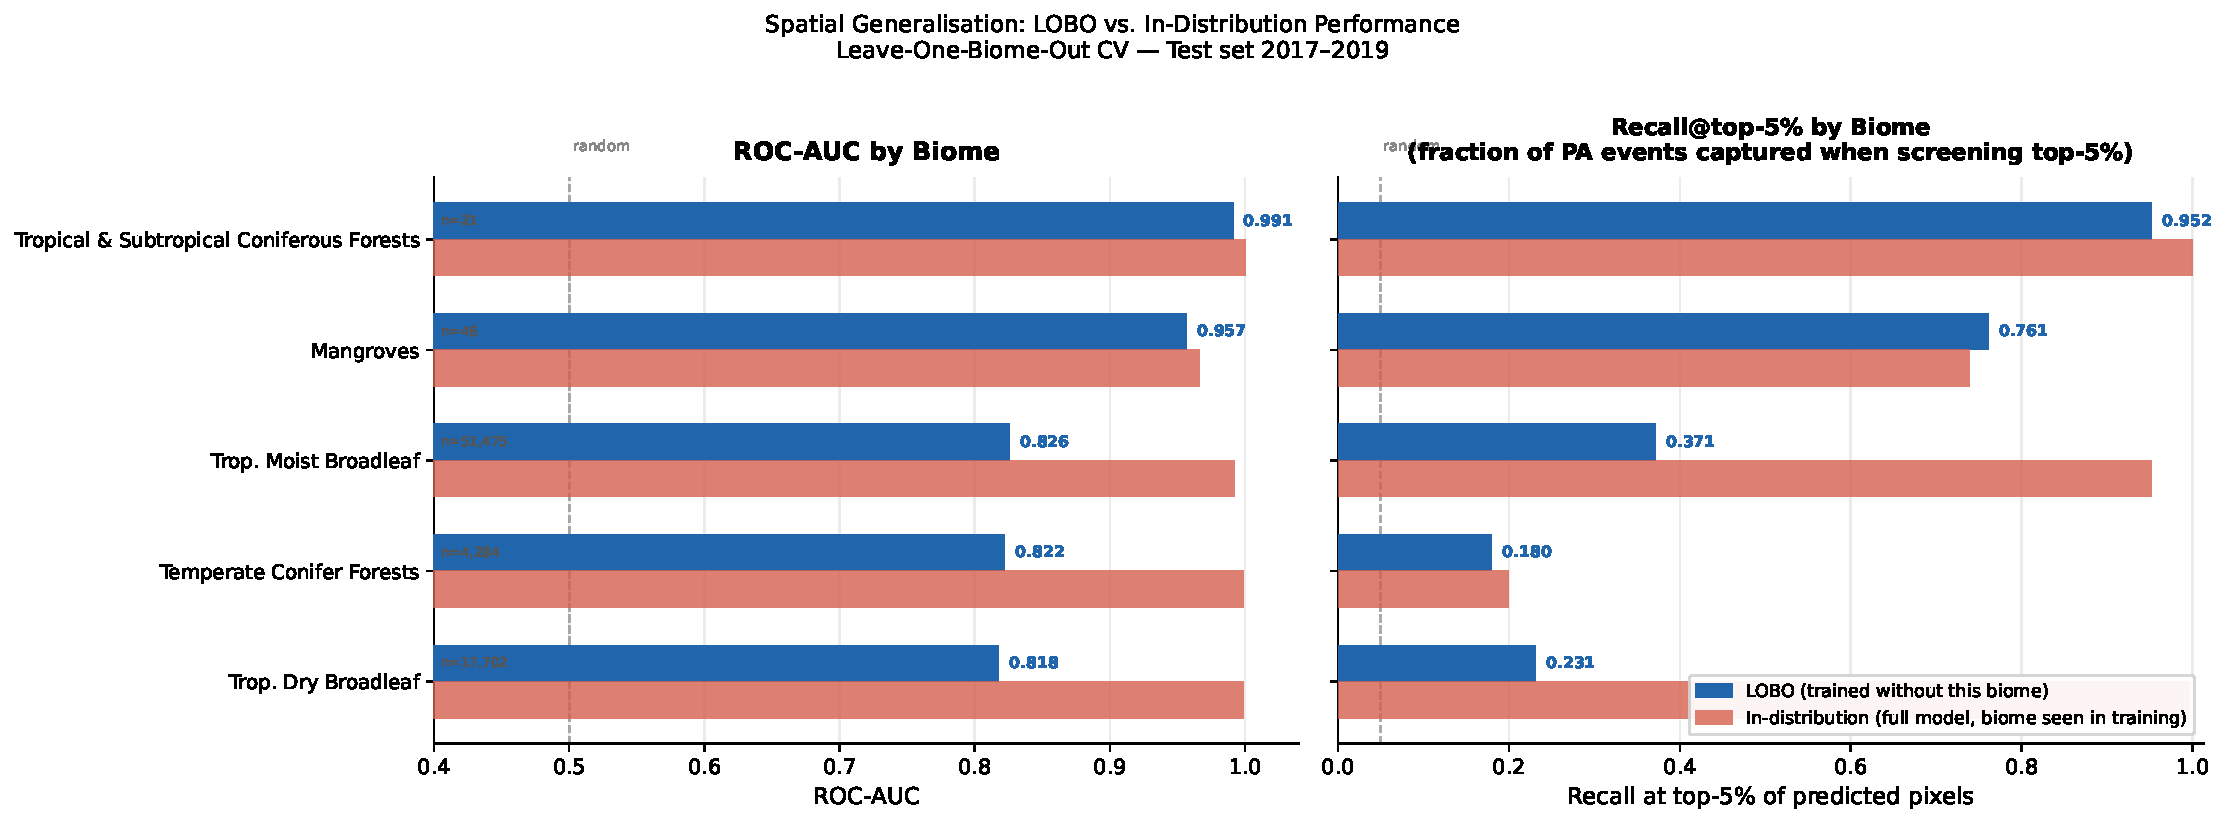
\includegraphics[width=\textwidth, keepaspectratio]{../outputs/se_asia/results/spatial_cv_visualisation/bar_lobo_performance_lgbm.pdf}
%\caption{Per-biome LOBO PR-AUC for Southeast Asia (LightGBM, test set 2017--2019).}
%\label{fig:lobo_seasia}
%\end{figure}

\begin{figure}[H]
\centering
\begin{subfigure}[t]{0.49\textwidth}
  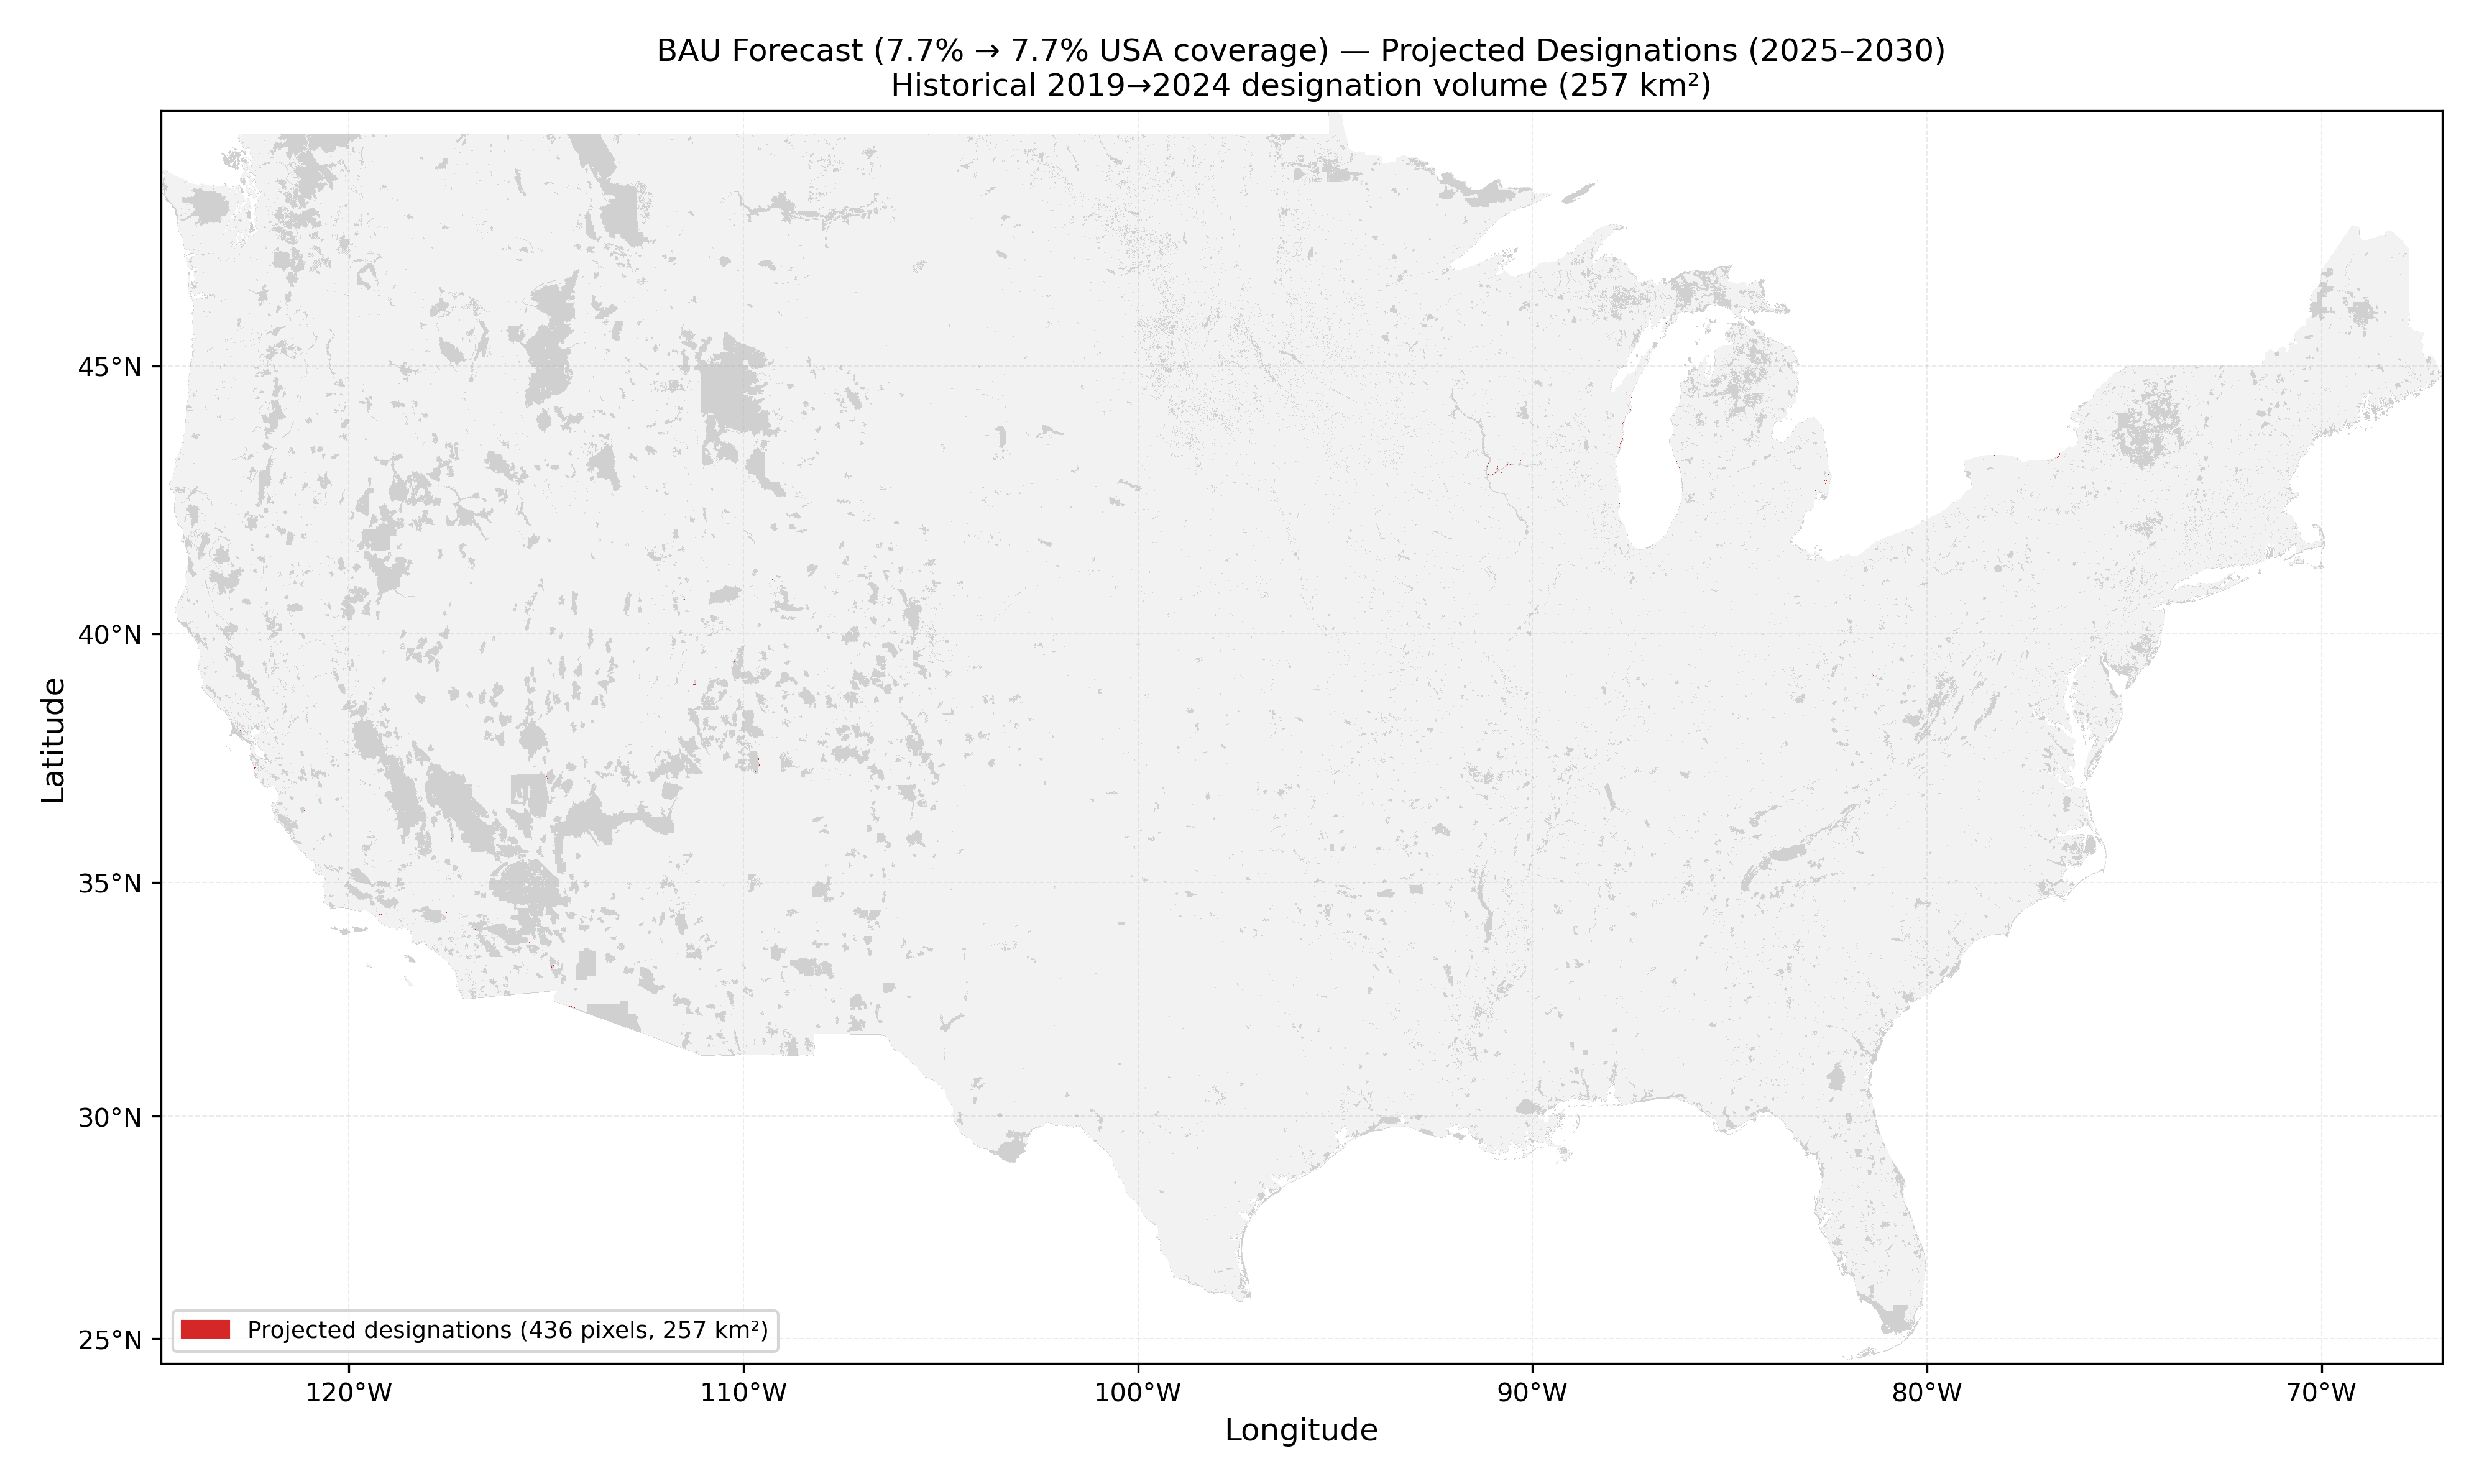
\includegraphics[width=\textwidth, keepaspectratio]{../outputs/usa/results/forward/lgbm/risk_map_bau.png}
  \caption{BAU scenario.}
  \label{fig:forward_usa_bau}
\end{subfigure}\hfill
\begin{subfigure}[t]{0.49\textwidth}
  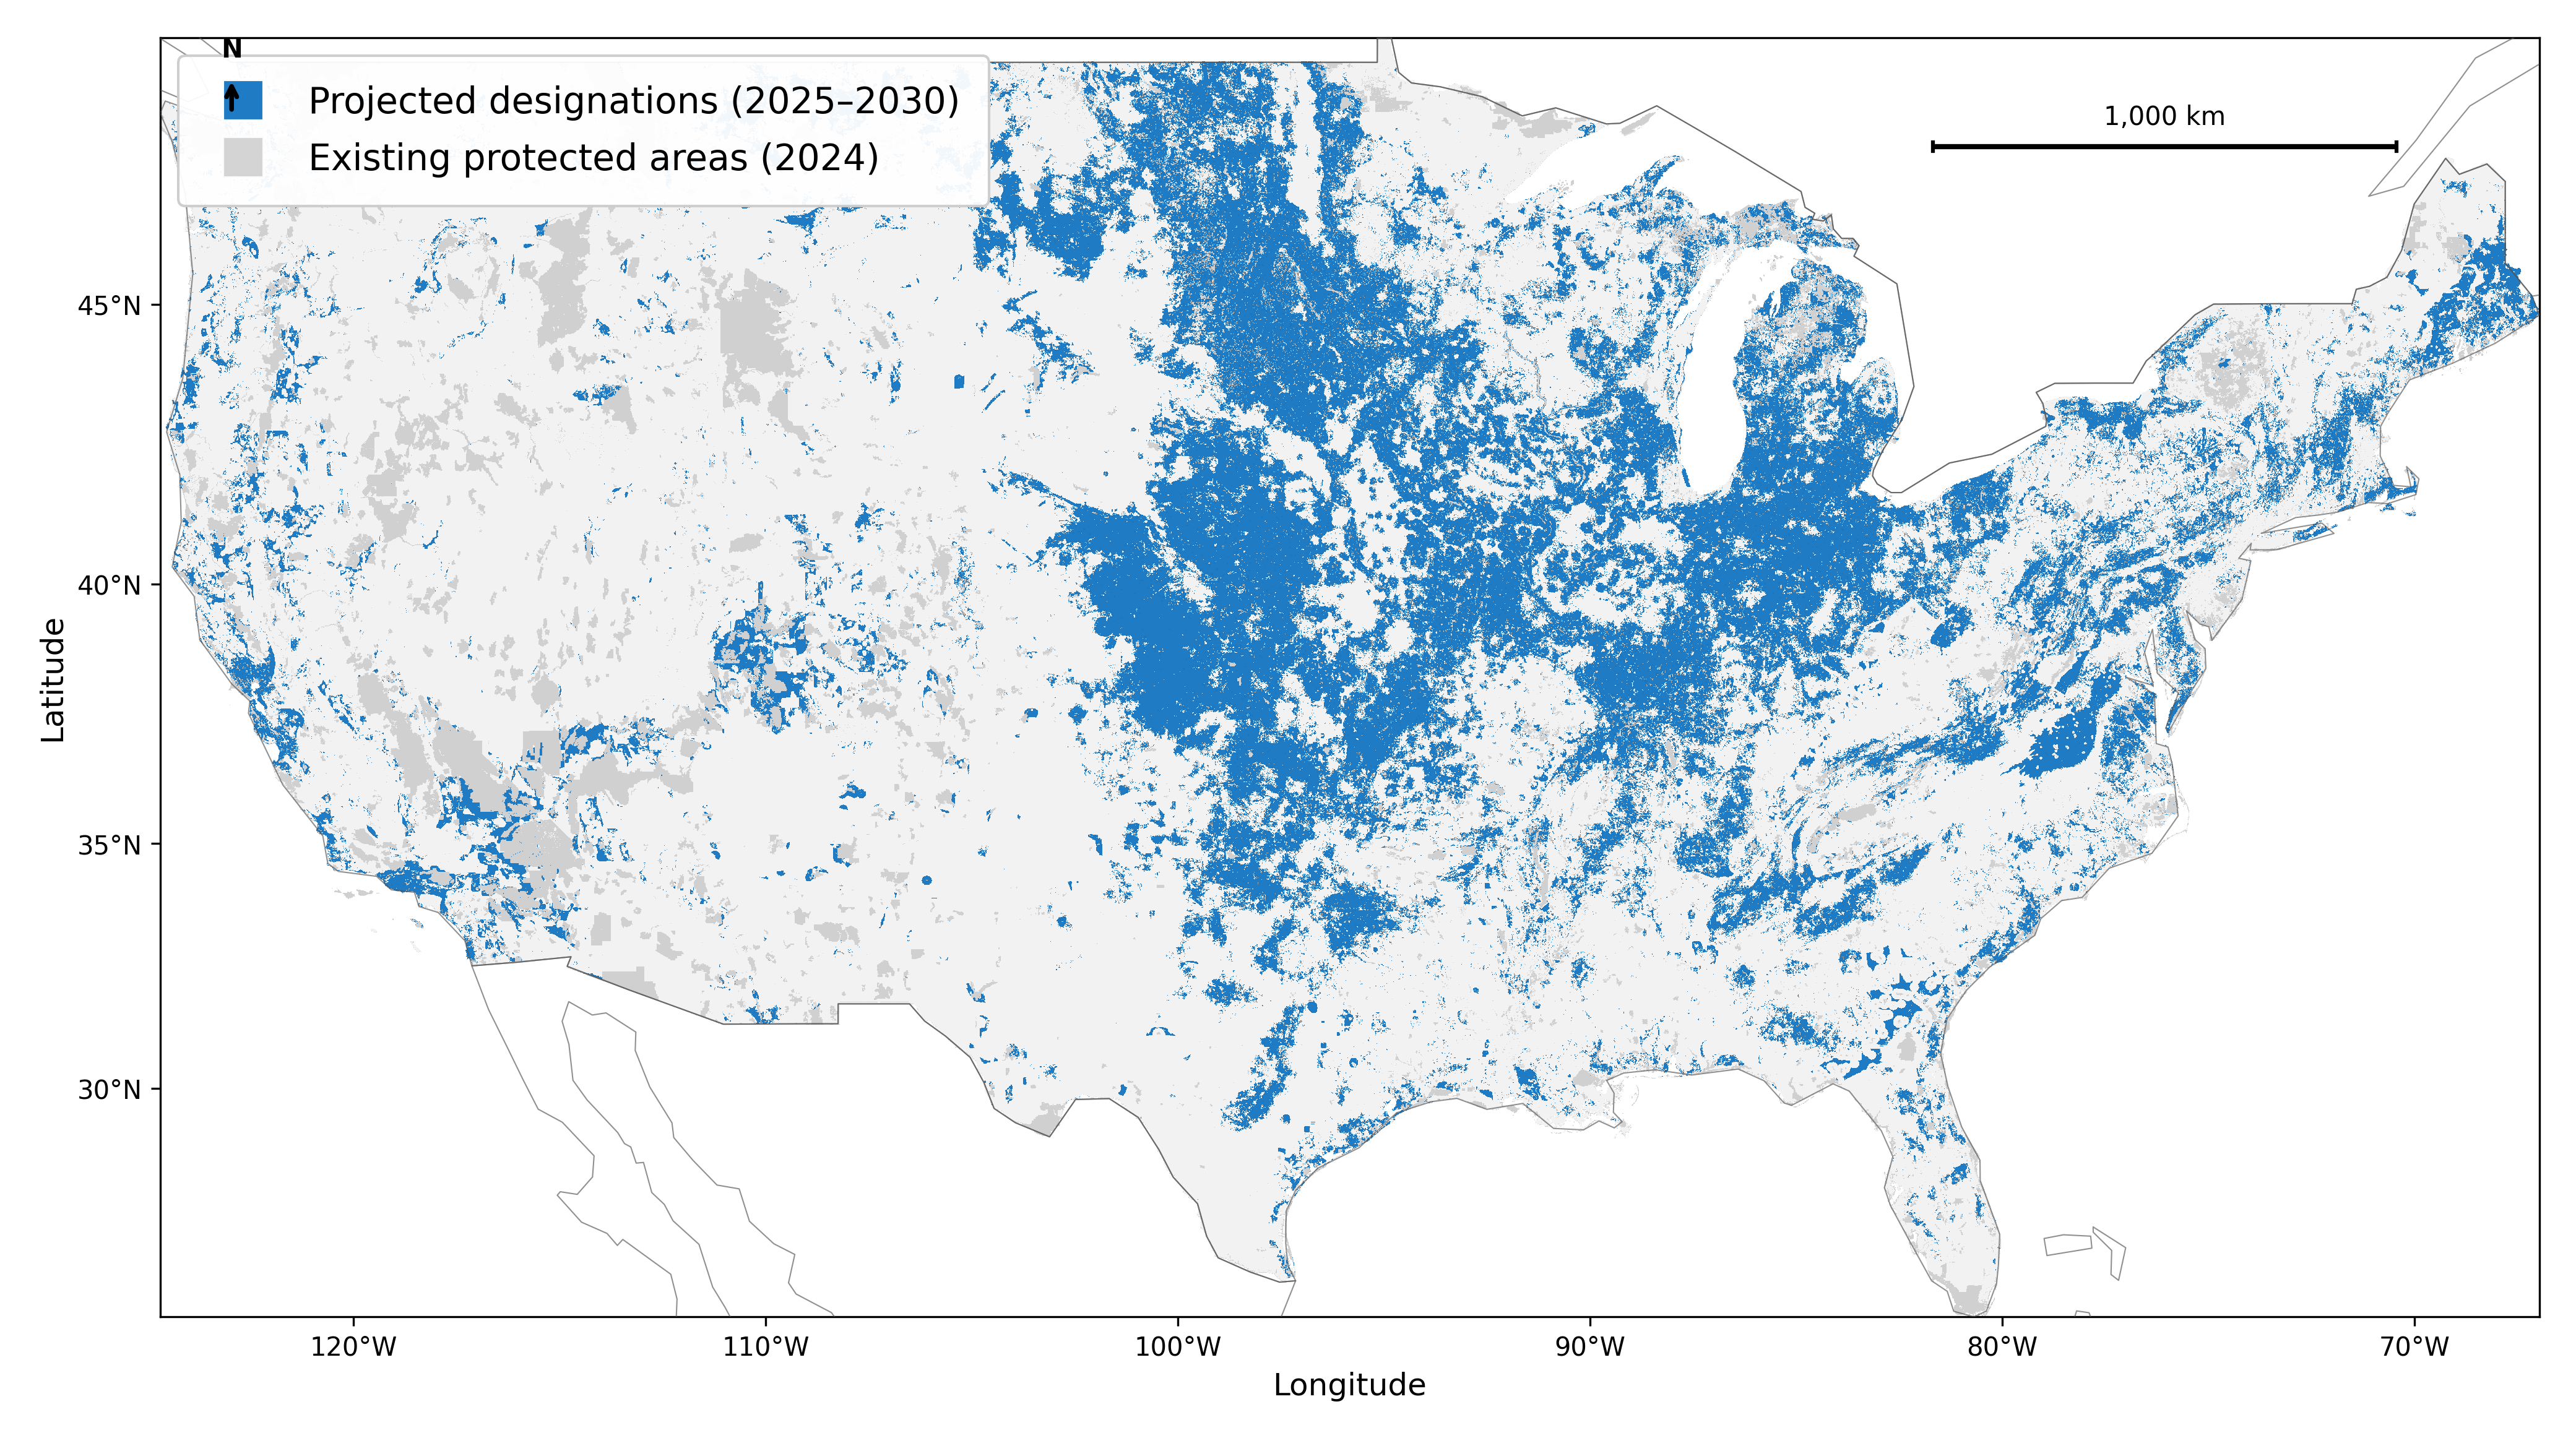
\includegraphics[width=\textwidth, keepaspectratio]{../outputs/usa/results/forward/lgbm/scenario_30x30.png}
  \caption{30$\times$30 scenario.}
  \label{fig:forward_usa_30x30}
\end{subfigure}
\caption{Forward projection for the United States under BAU and 30$\times$30 scenarios.
Coloured clusters indicate high-probability pixels; grey shows the current
protected-area network. Designation concentrates in the arid West (BLM and National
Forest lands) and the Pacific Northwest.}
\label{fig:forward_usa}
\end{figure}

\begin{figure}[H]
\centering
\begin{subfigure}[t]{0.49\textwidth}
  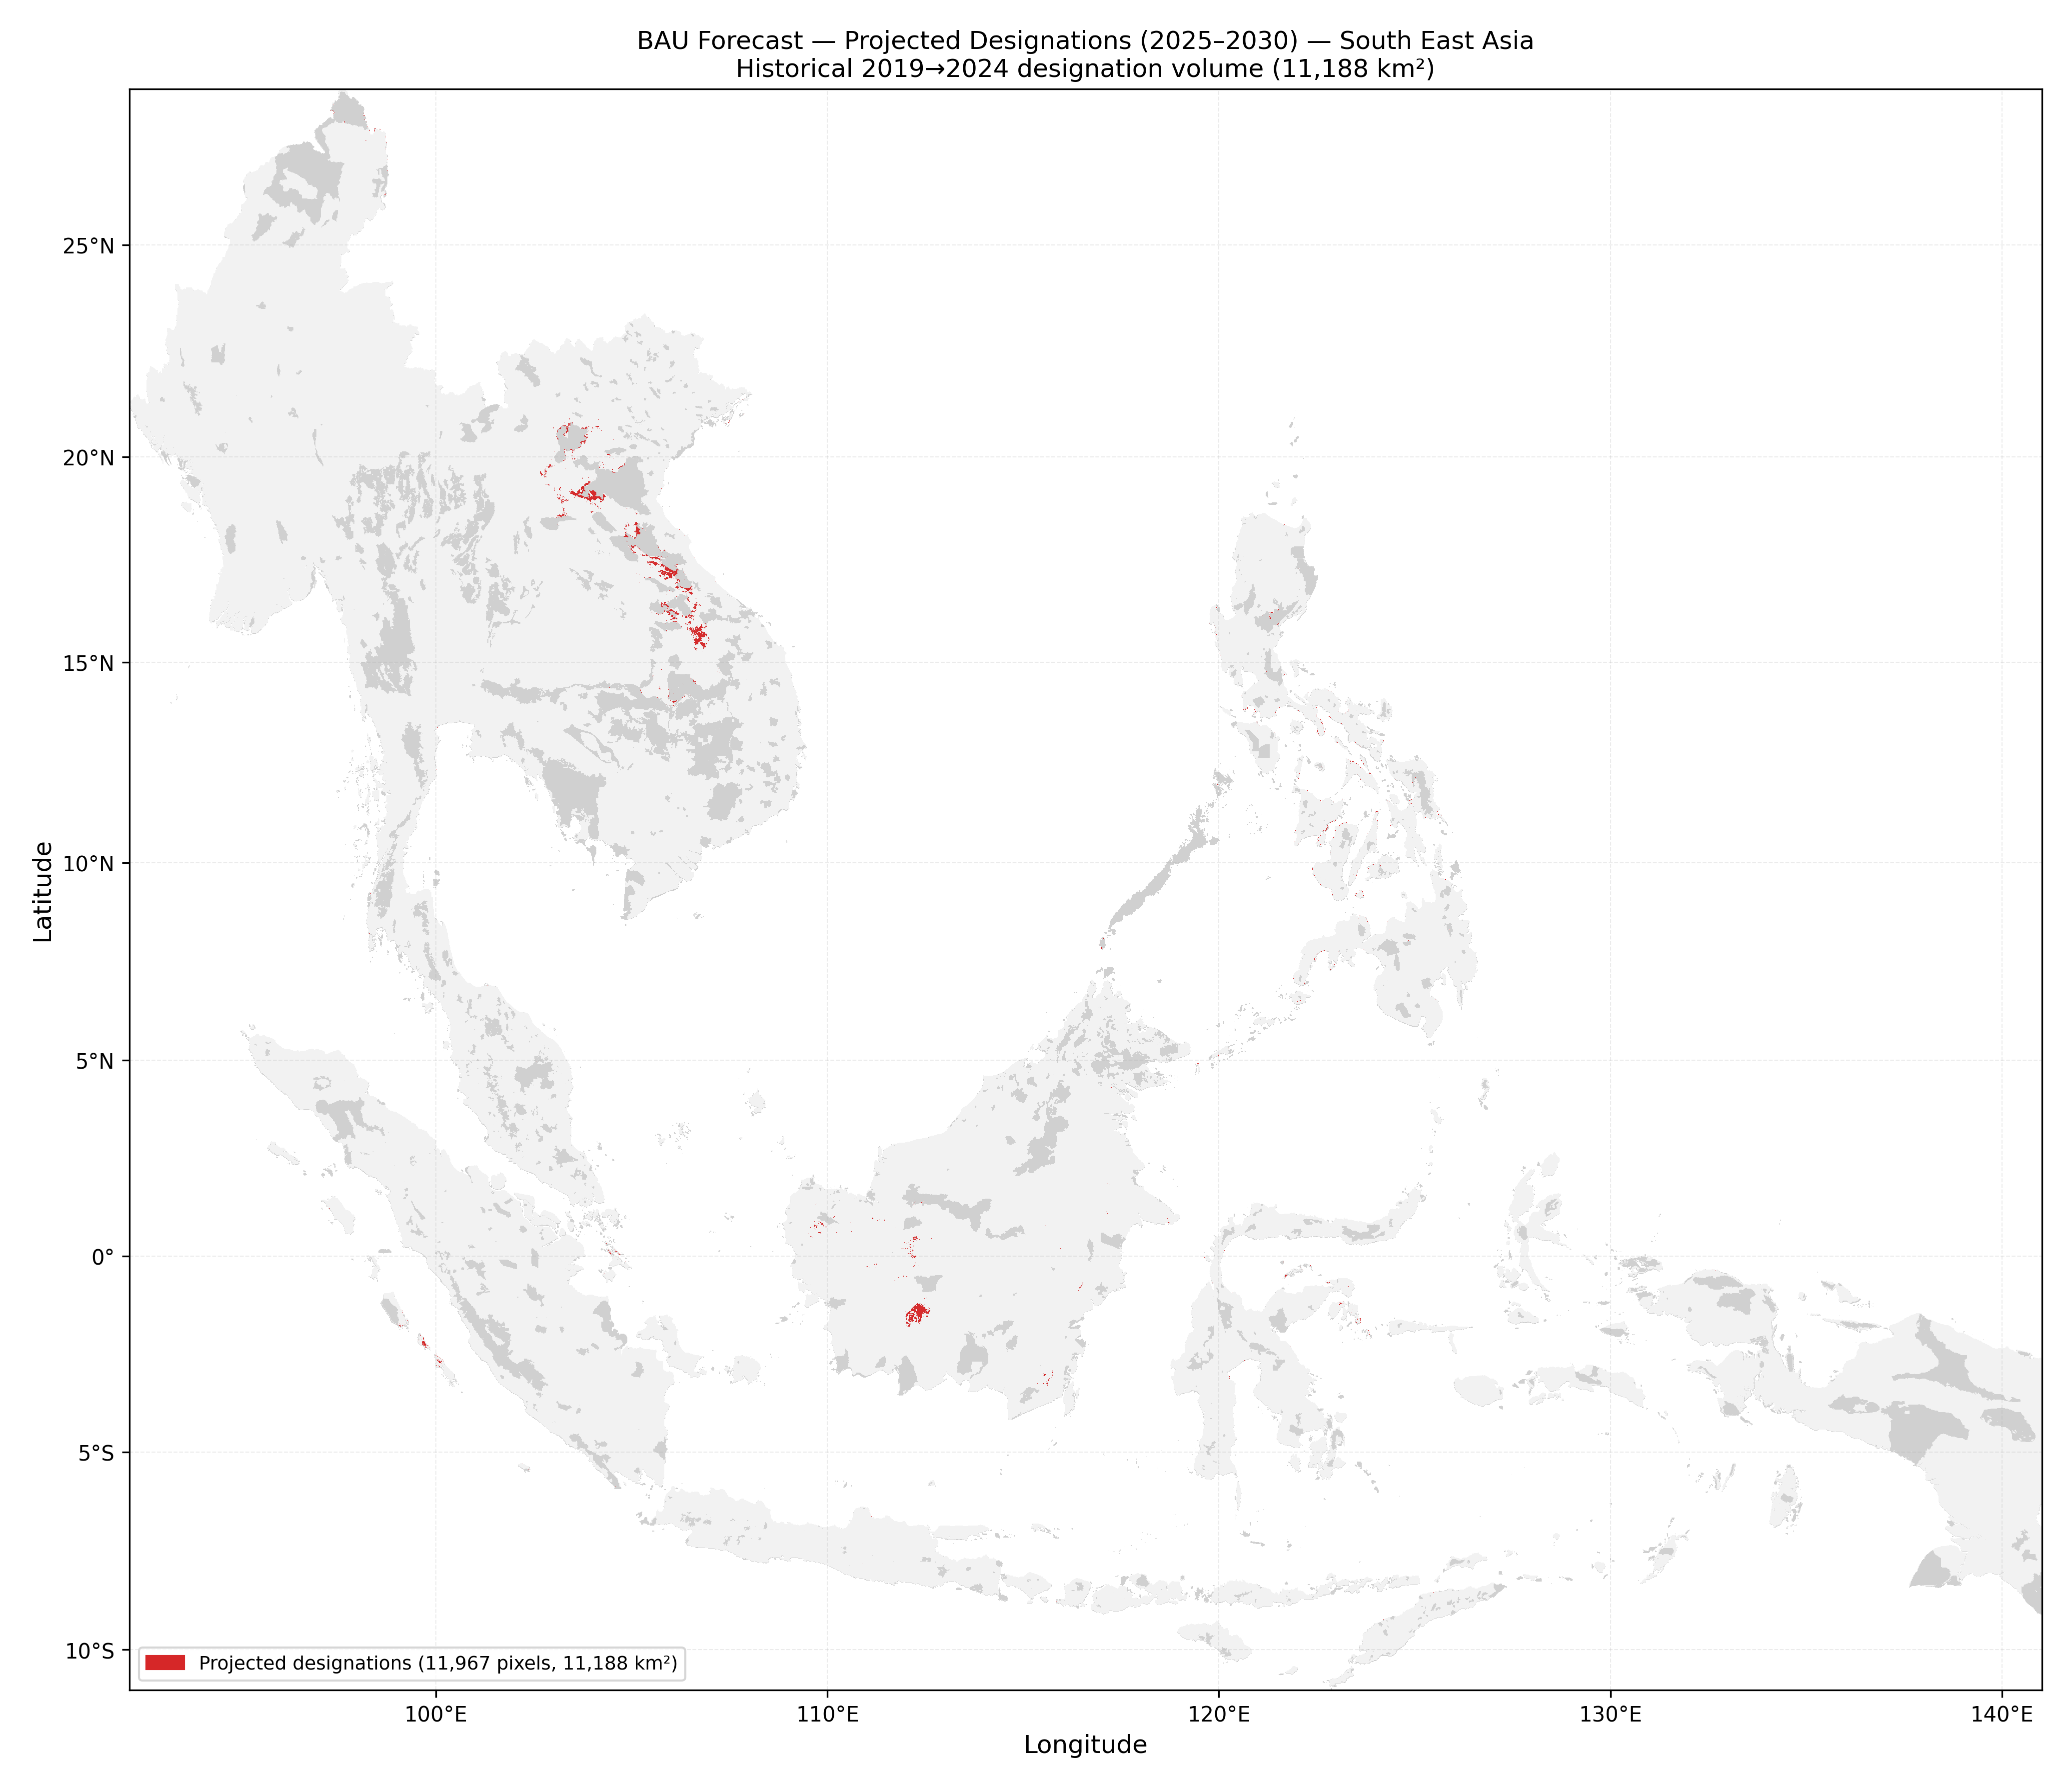
\includegraphics[width=\textwidth, keepaspectratio]{../outputs/se_asia/results/forward/lgbm/risk_map_bau.png}
  \caption{BAU scenario.}
  \label{fig:forward_seasia_bau}
\end{subfigure}\hfill
\begin{subfigure}[t]{0.49\textwidth}
  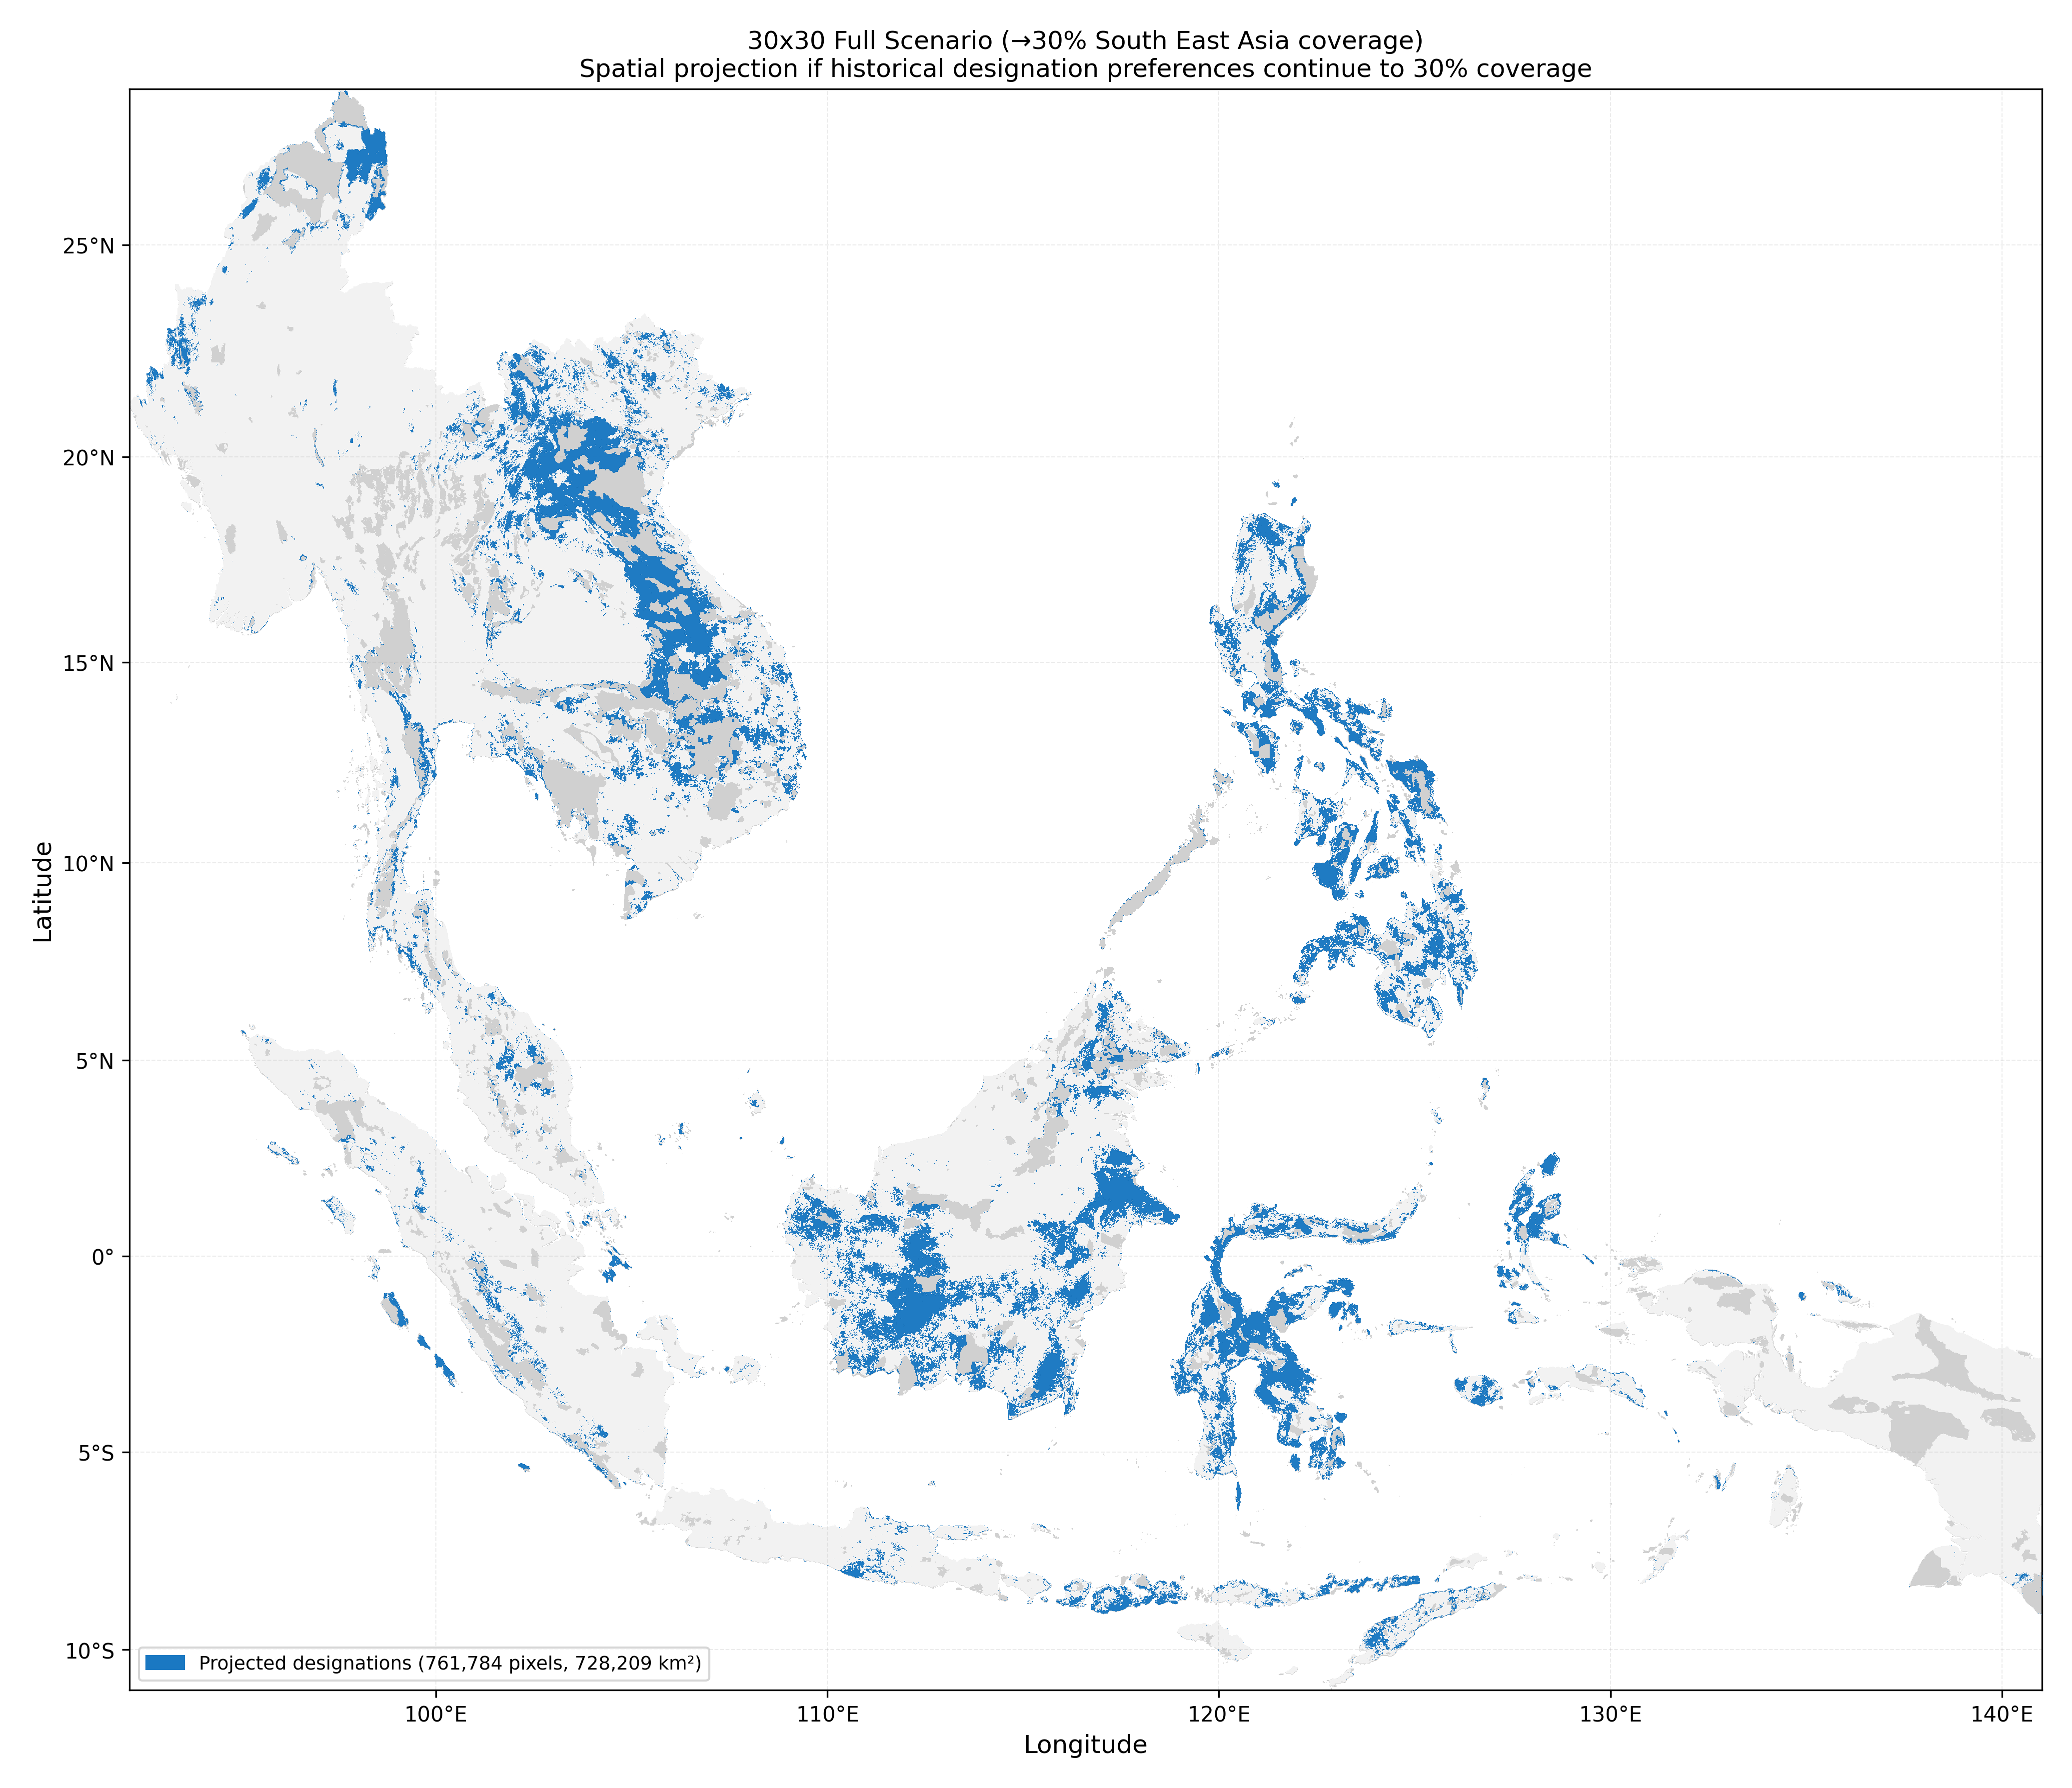
\includegraphics[width=\textwidth, keepaspectratio]{../outputs/se_asia/results/forward/lgbm/scenario_30x30.png}
  \caption{30$\times$30 scenario.}
  \label{fig:forward_seasia_30x30}
\end{subfigure}
\caption{Forward projection for Southeast Asia under BAU and 30$\times$30 scenarios.
The limited number of clusters (9 total) reflects the concentration of
high-probability pixels in large forested upland areas in Borneo and Sumatra.}
\label{fig:forward_seasia}
\end{figure}

\begin{figure}[H]
  \centering
  \begin{subfigure}[t]{0.49\textwidth}
    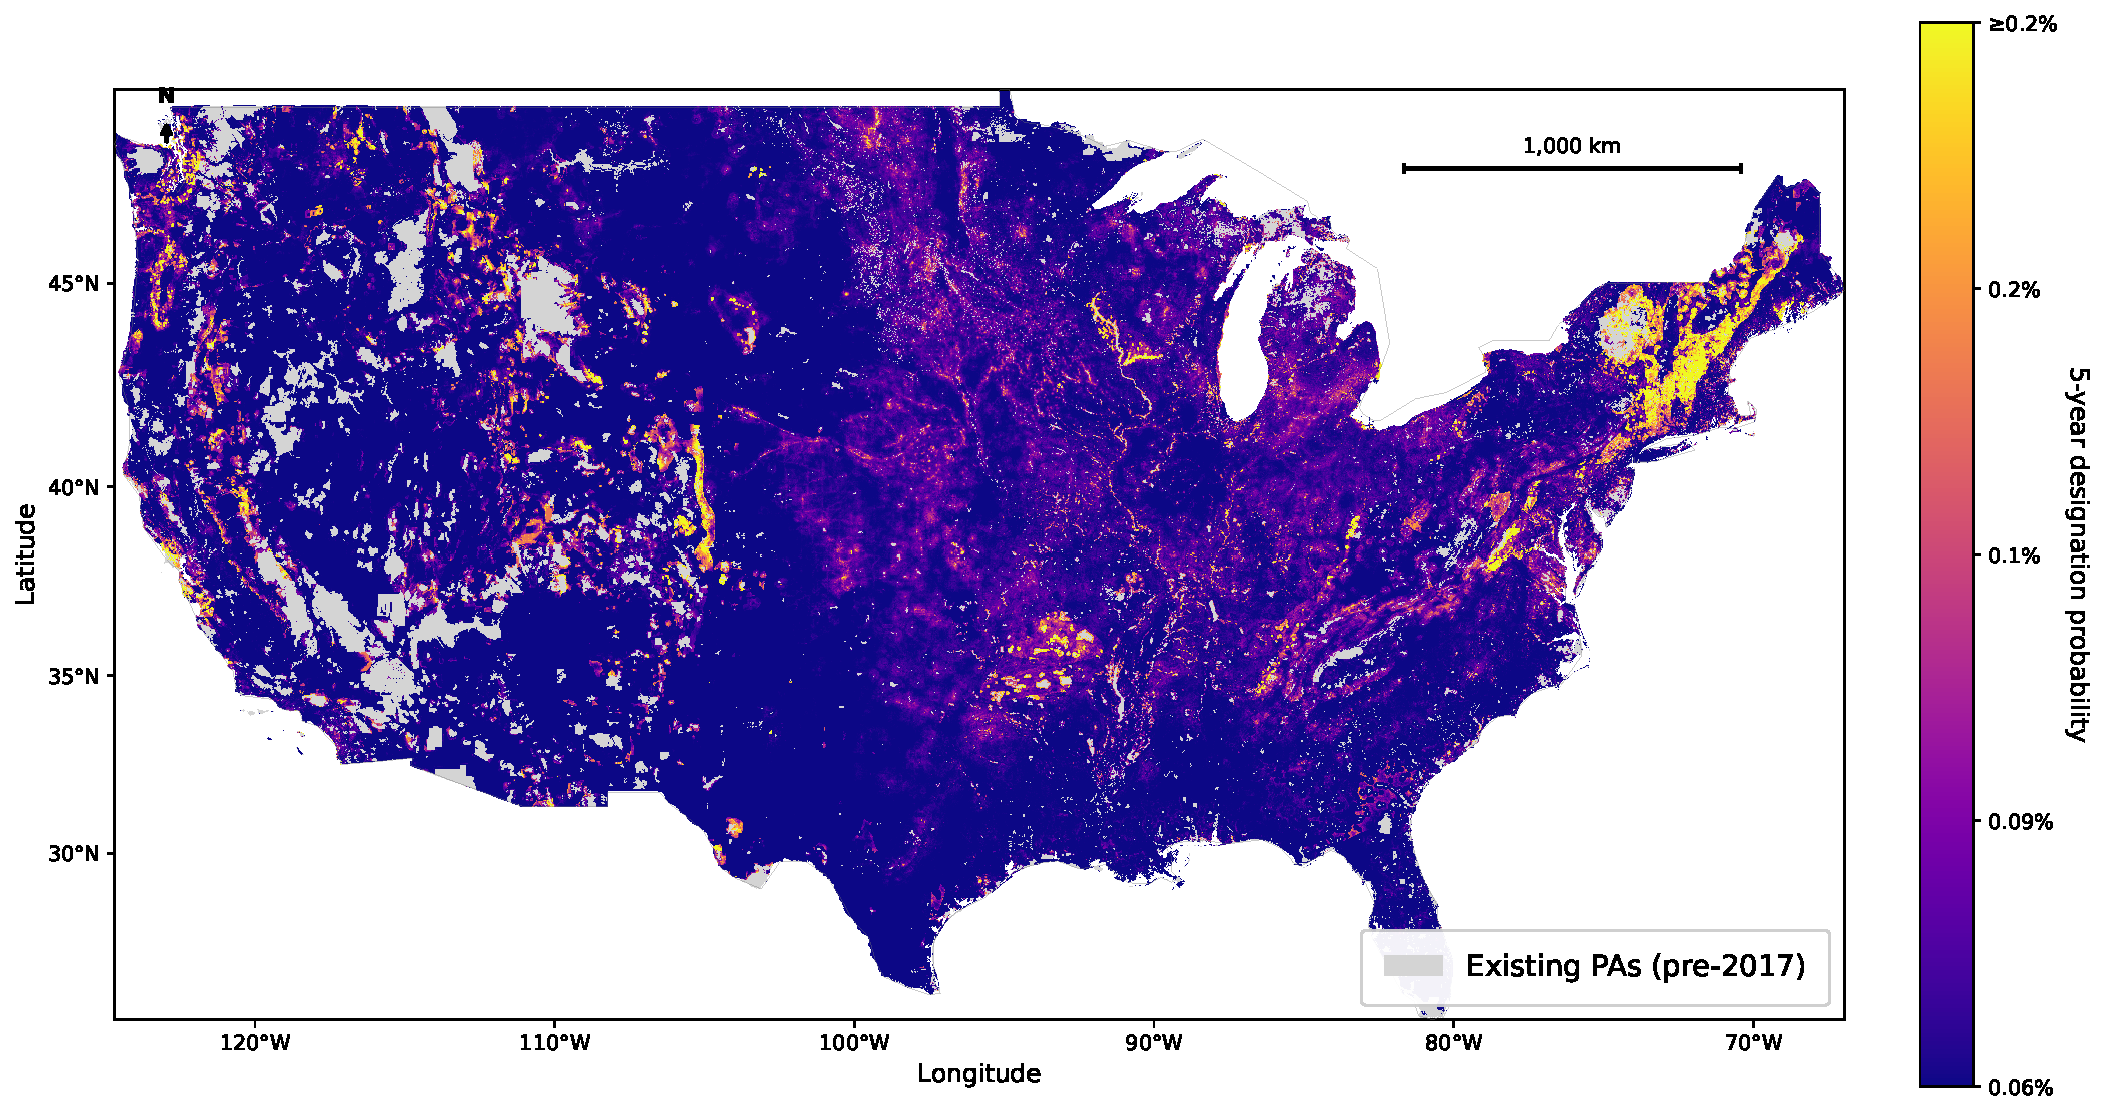
\includegraphics[width=\textwidth, keepaspectratio]{../outputs/usa/results/model2_lgbm/probability_map.pdf}
    \caption{United States. Higher probabilities concentrate in the arid West where Bureau of
    Land Management public land dominates. Note the compressed probability scale relative
    to South America, reflecting the 20$\times$ lower positive rate ($\approx$0.04\%).}
    \label{fig:probmap_usa}
  \end{subfigure}\hfill
  \begin{subfigure}[t]{0.49\textwidth}
    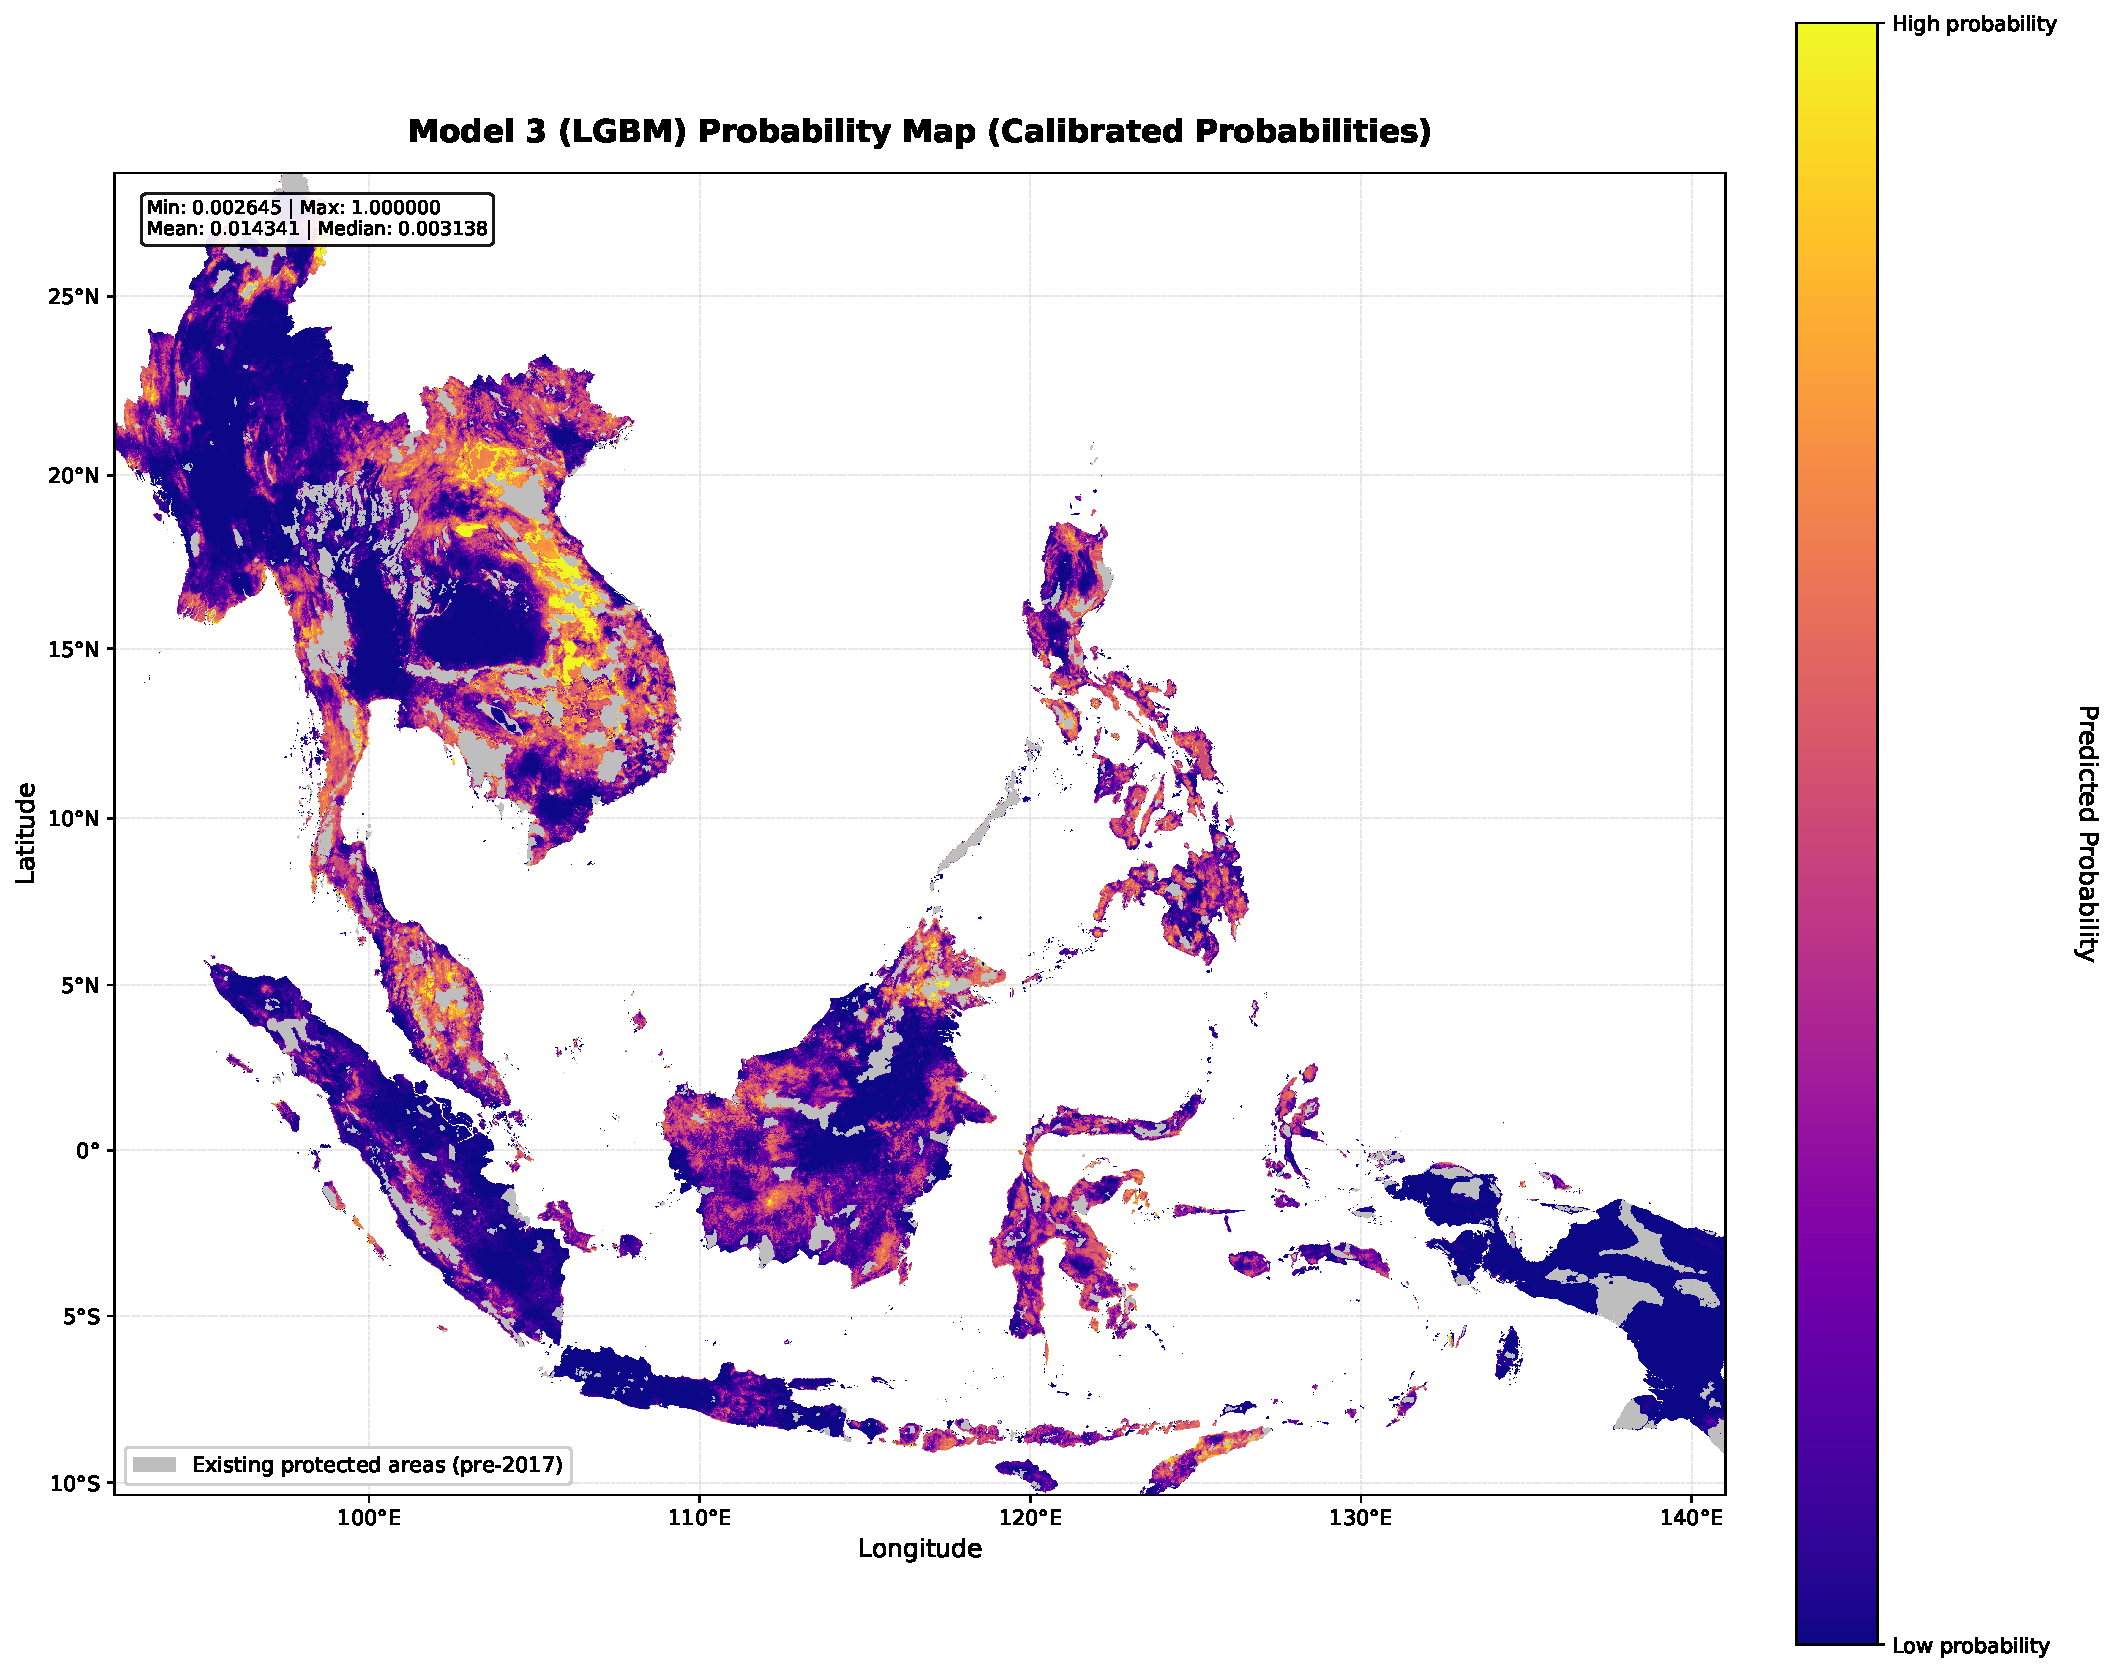
\includegraphics[width=\textwidth, keepaspectratio]{../outputs/se_asia/results/model3_lgbm/probability_map.pdf}
    \caption{Southeast Asia. High-probability pixels cluster in the forested uplands of Borneo,
    Sumatra, and peninsular Malaysia, reflecting the strong elevation and canopy-cover
    signal in this region.}
    \label{fig:probmap_seasia}
  \end{subfigure}
  \caption{Predicted 5-year PA designation probability (LightGBM, deployment model) for the United States and Southeast Asia.}
  \label{fig:probmaps_usa_seasia}
\end{figure}

\begin{figure}[H]
\centering
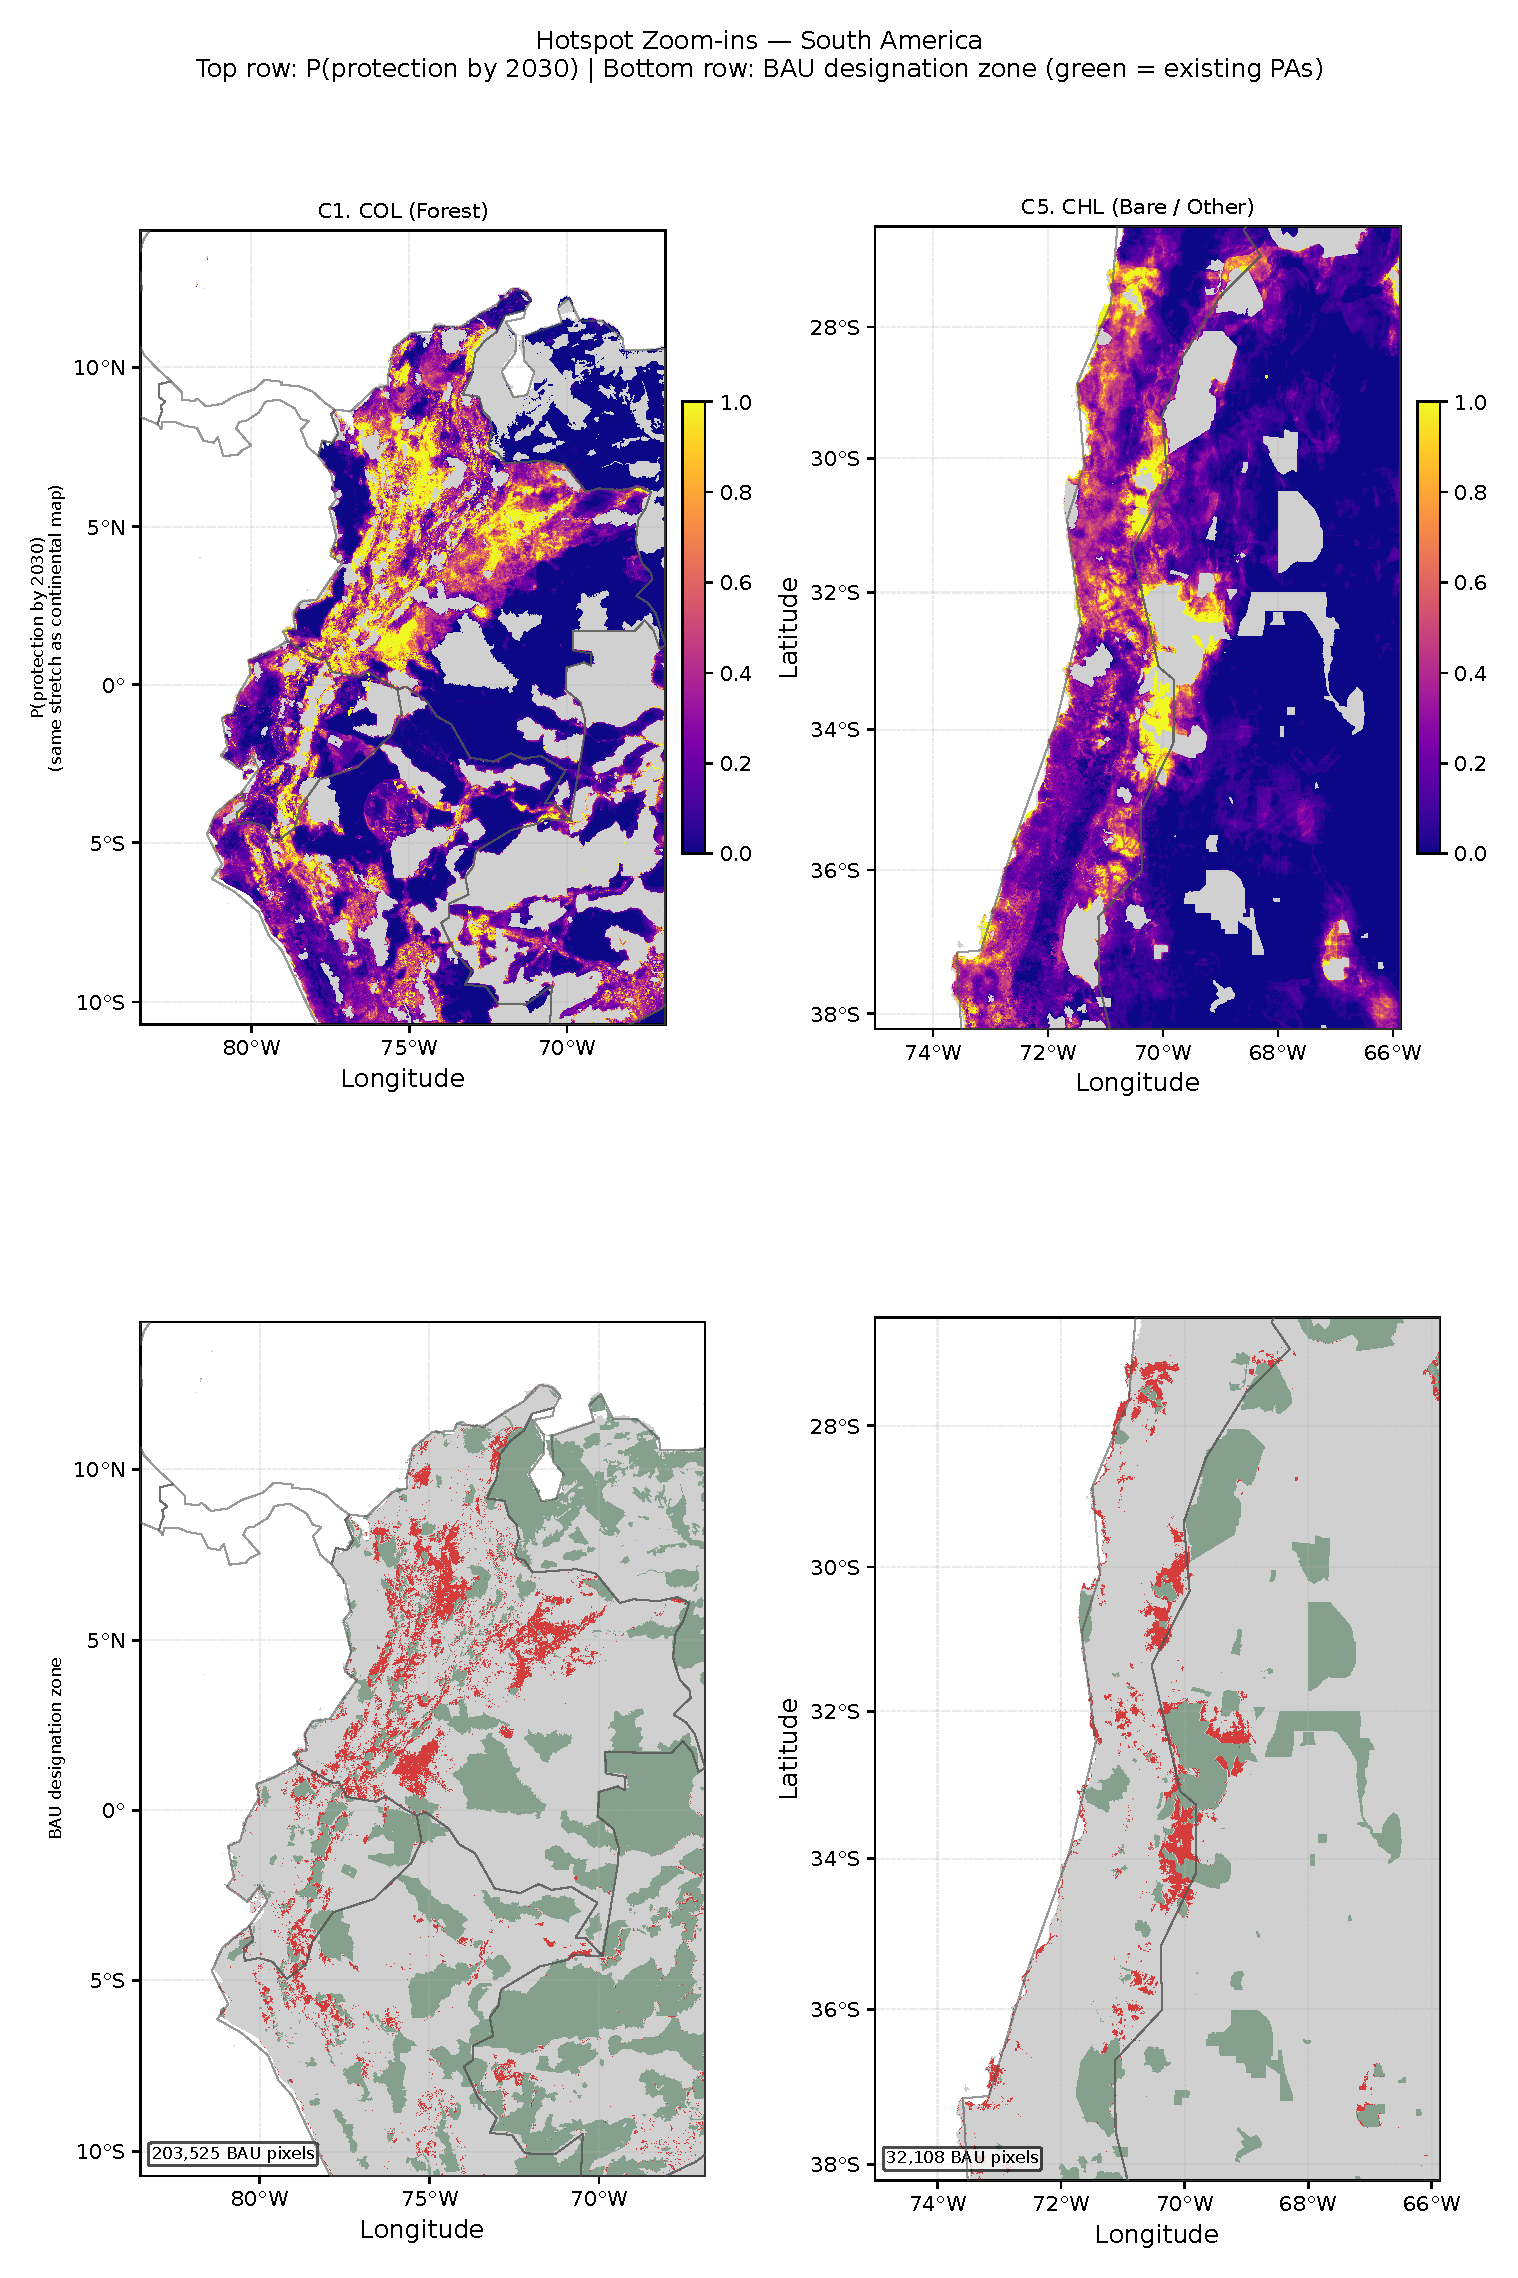
\includegraphics[width=0.60\textwidth, keepaspectratio]{../outputs/south_america/results/forward/lgbm/hotspot_maps.pdf}
\caption{Hotspot zoom-ins for South America (LightGBM, BAU scenario).
Top row: predicted designation probability by 2030. Bottom row: BAU designation zone
(red), existing PAs in green, country borders in grey. Left: Colombian Amazon cluster
(C1, highest-ranked BAU hotspot). Right: central Chilean cluster (C5, Andean foothills
Bare/Other land-cover regime).}
\label{fig:hotspot_sa}
\end{figure}

\begin{figure}[H]
\centering
\begin{subfigure}[t]{0.32\textwidth}
  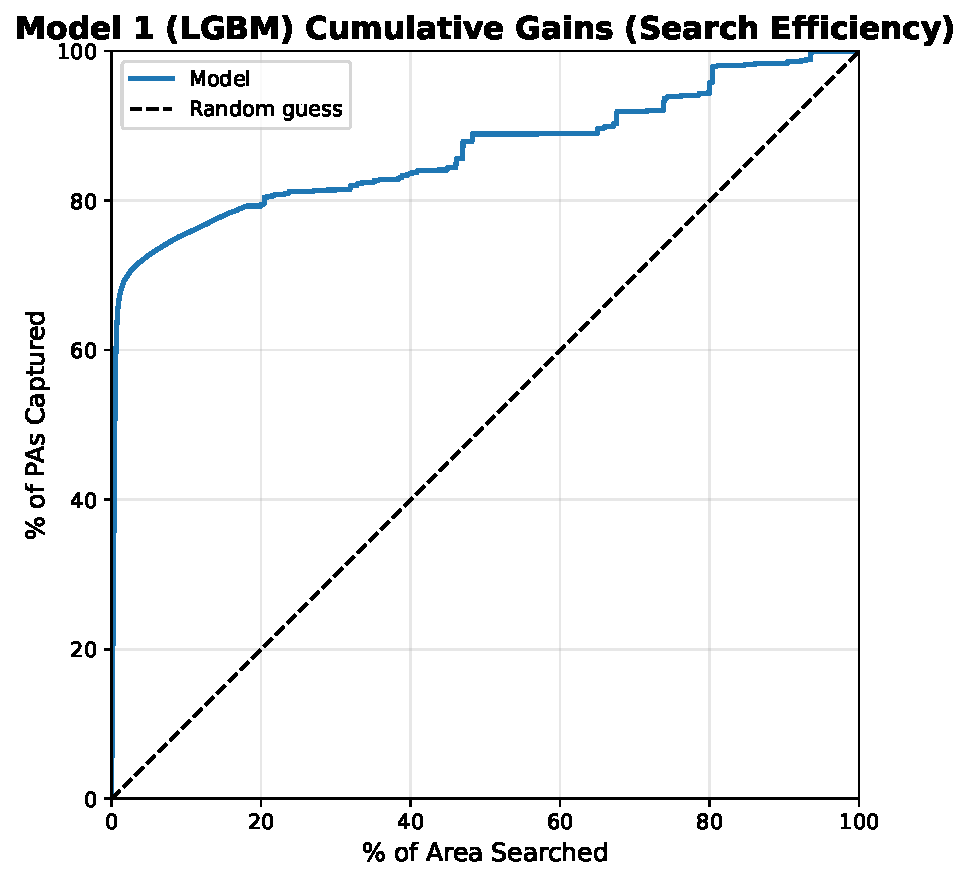
\includegraphics[width=\textwidth, keepaspectratio]{../outputs/south_america/results/model1_lgbm/cumulative_gains.pdf}
  \caption{South America (LightGBM)}
  \label{fig:cumgains_sa}
\end{subfigure}\hfill
\begin{subfigure}[t]{0.32\textwidth}
  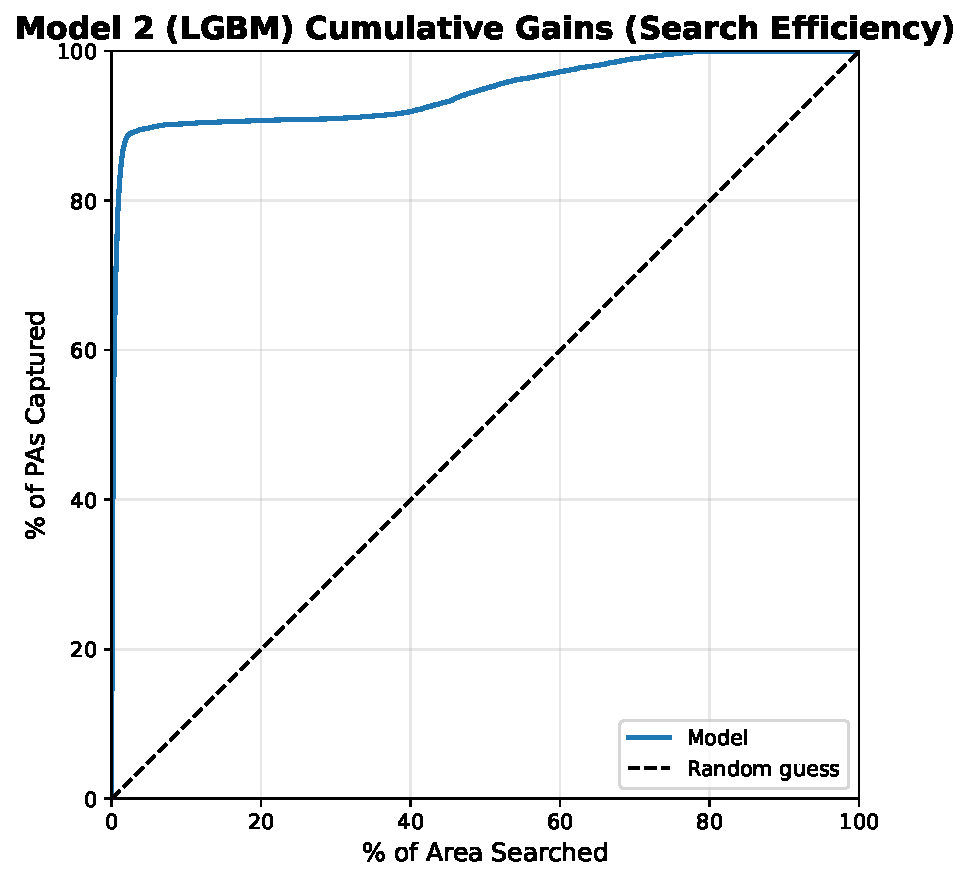
\includegraphics[width=\textwidth, keepaspectratio]{../outputs/usa/results/model2_lgbm/cumulative_gains.pdf}
  \caption{United States (LightGBM)}
  \label{fig:cumgains_usa}
\end{subfigure}\hfill
\begin{subfigure}[t]{0.32\textwidth}
  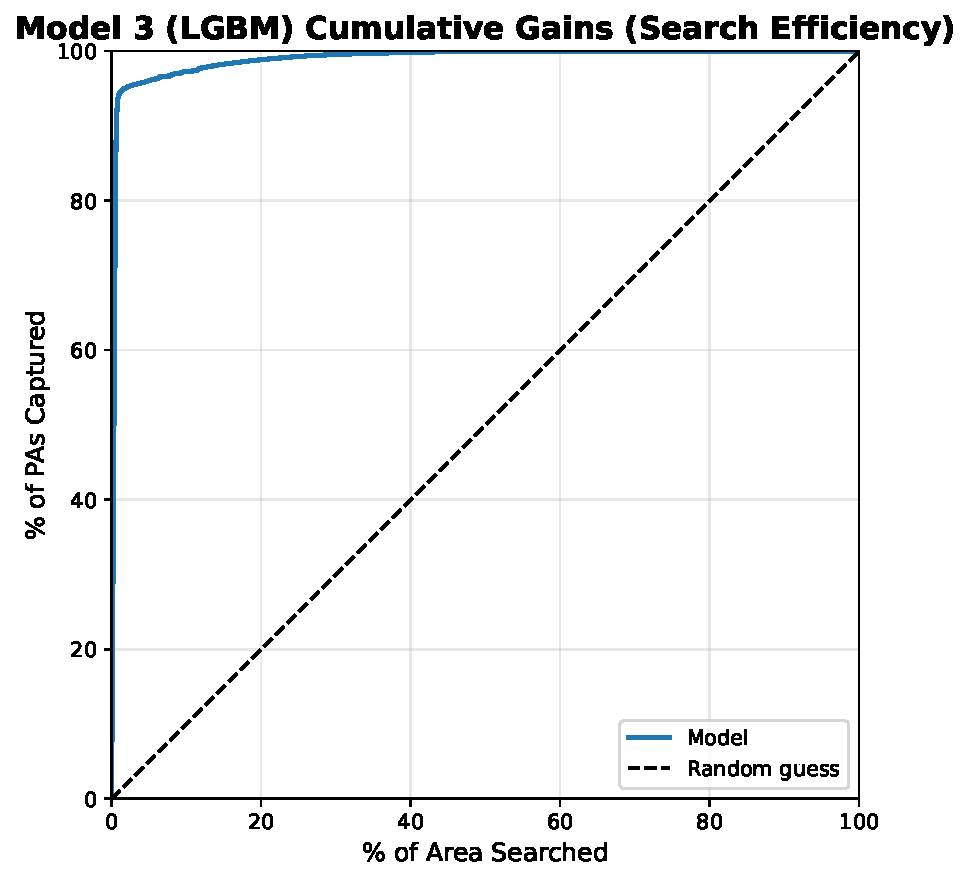
\includegraphics[width=\textwidth, keepaspectratio]{../outputs/se_asia/results/model3_lgbm/cumulative_gains.pdf}
  \caption{Southeast Asia (LightGBM)}
  \label{fig:cumgains_seasia}
\end{subfigure}
\caption{Cumulative gains charts for all three regions (LightGBM, test period 2017--2019).
Each curve shows the fraction of all pixel-year positive observations captured as a
function of the fraction of pixels scored, ranked by predicted probability. The dashed
diagonal represents a random scorer (no skill).}
\label{fig:cumgains_all}
\end{figure}

\begin{figure}[H]
\centering
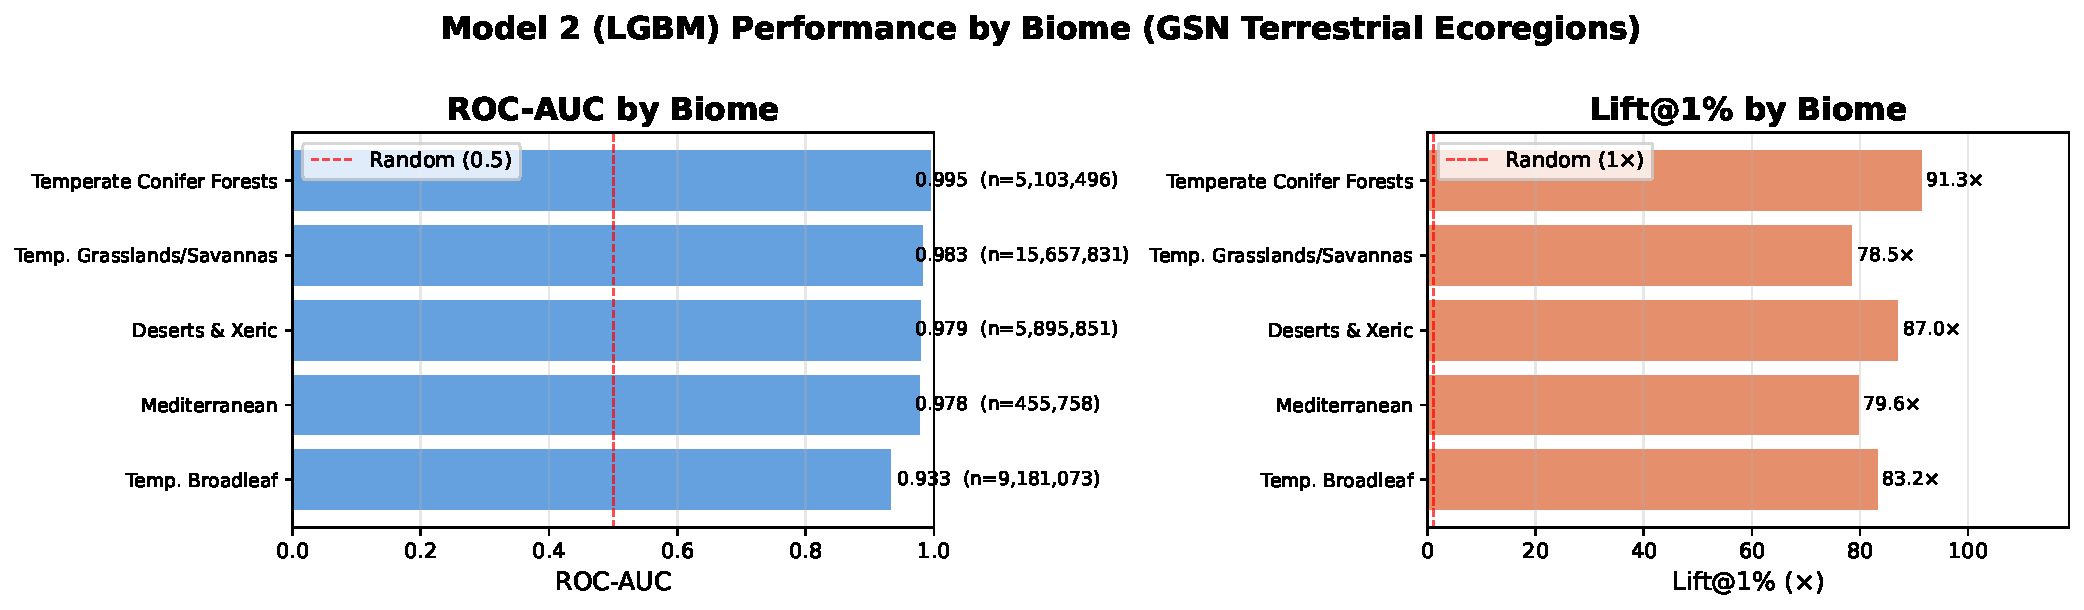
\includegraphics[width=\textwidth, keepaspectratio]{../outputs/usa/results/model2_lgbm/biome_breakdown.pdf}
\caption{United States biome-stratified performance (full production LightGBM model,
test set 2017--2019). Each biome is evaluated using scores from the model trained on
all biomes simultaneously. ROC-AUC is uniformly high across biomes (0.93--0.995)
while Precision@1\% is uniformly suppressed by the near-zero national positive rate
($\approx$0.04\%), reflecting the base-rate effect rather than poor discrimination.}
\label{fig:biome_breakdown_usa}
\end{figure}

\begin{figure}[H]
\centering
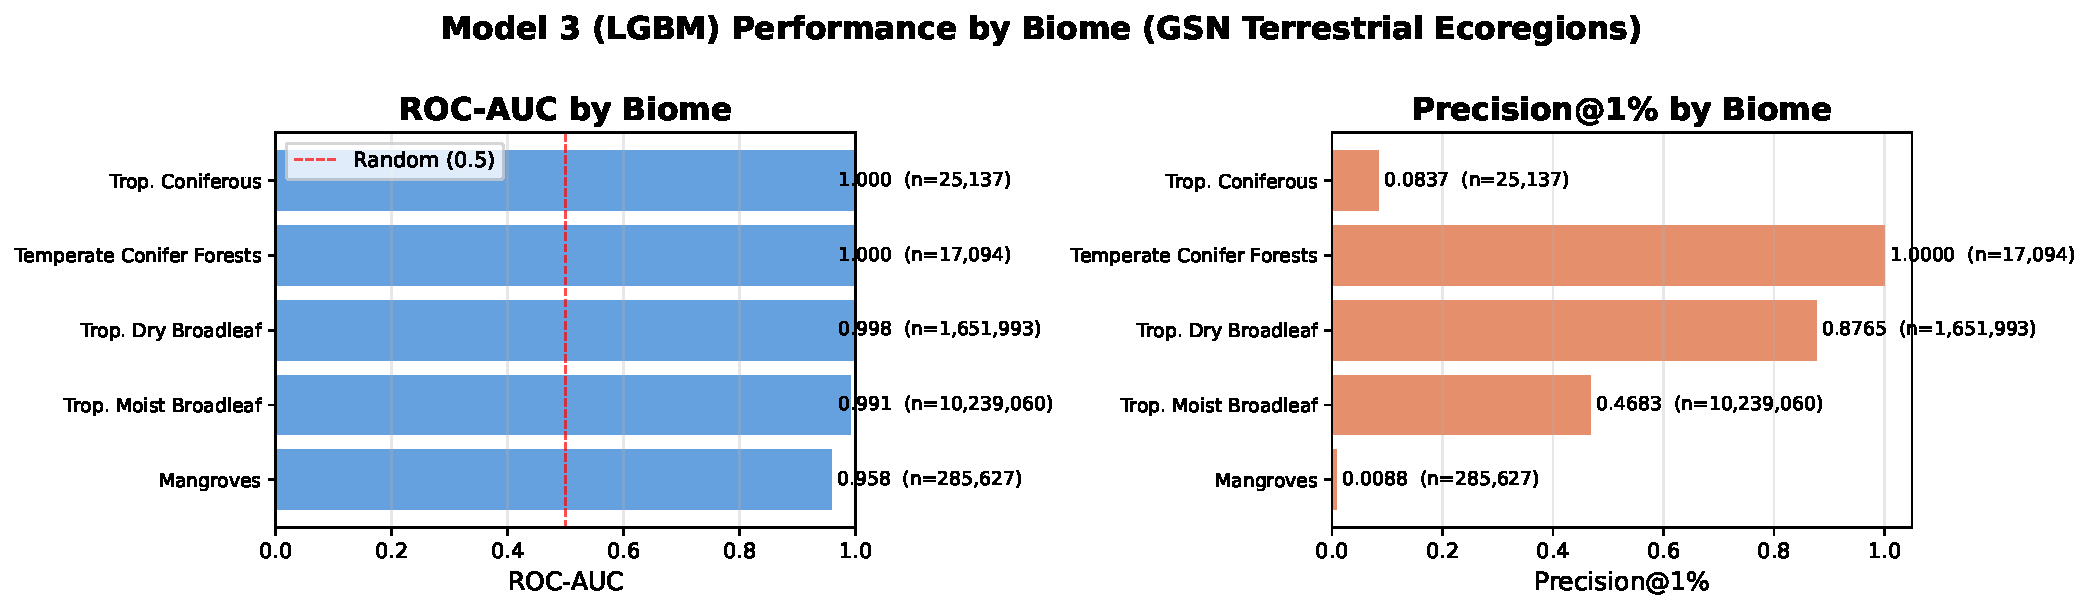
\includegraphics[width=\textwidth, keepaspectratio]{../outputs/se_asia/results/model3_lgbm/biome_breakdown.pdf}
\caption{Southeast Asia biome-stratified performance (full production LightGBM model,
test set 2017--2019). Each biome is evaluated using scores from the model trained on
all biomes simultaneously. Tropical \& Subtropical Dry Broadleaf Forests and Temperate
Conifer Forests achieve both high discrimination and high absolute precision (Precision@1\%
of 0.877 and 1.0 respectively), driven by their substantially higher positive rates
(1.07\% and 25\%).}
\label{fig:biome_breakdown_seasia}
\end{figure}

\section{SHAP Dependence Plots}
\label{app:shap_dep}

SHAP dependence plots show how a single feature's value affects its SHAP contribution
to the model's log-odds output. Each point is one observation from the SHAP sample;
the $x$-axis is the raw feature value, the $y$-axis is the SHAP value (positive =
increases predicted designation probability, negative = decreases it). The colour
of each point encodes the SHAP value of the most strongly interacting secondary
feature, revealing joint effects. The following plots illustrate the three features
with the most interpretively distinctive marginal effects for the South America
LightGBM model.

\begin{figure}[H]
\centering
\begin{subfigure}[t]{0.48\textwidth}
  \centering
  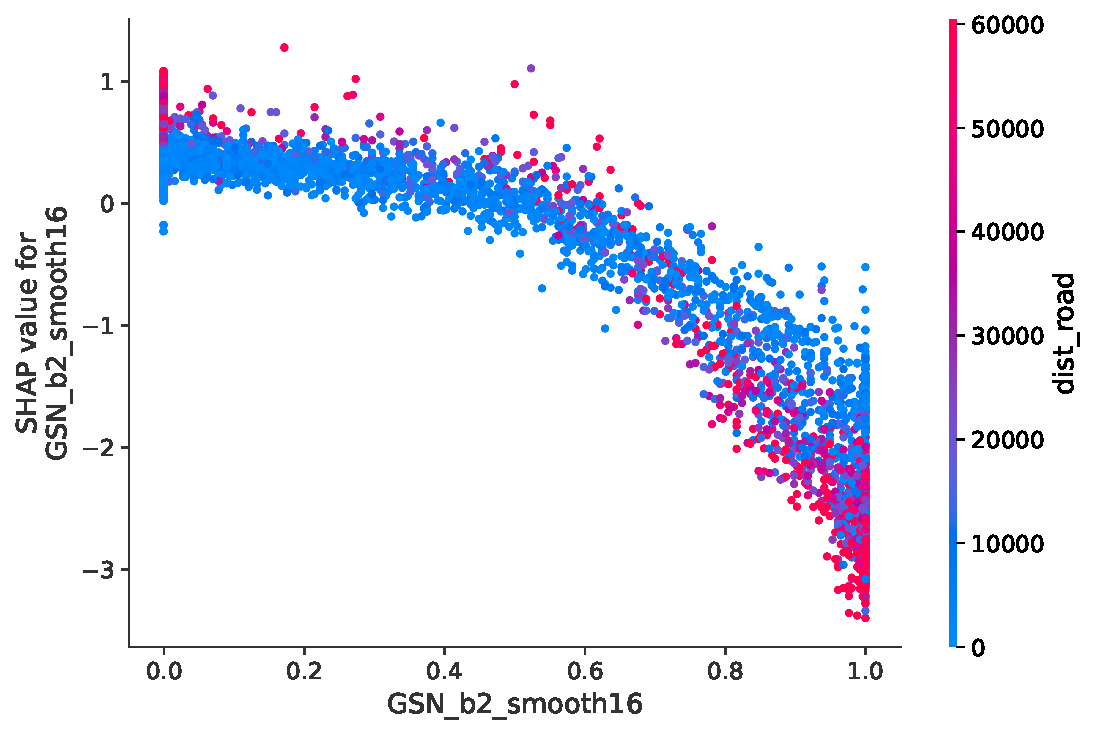
\includegraphics[width=\textwidth, keepaspectratio]{../outputs/south_america/results/model1_lgbm/shap_dep_GSN_b2_smooth16.pdf}
  \caption{SHAP dependence plot for \texttt{GSN\_b2\_smooth16} (GSN high-biodiversity
  indicator, $16 \times 16$ km neighbourhood mean). The positive relationship shows
  that pixels in globally significant biodiversity areas carry a higher marginal
  SHAP contribution towards designation, on average across the model's feature
  interactions. Colour indicates the SHAP value of a secondary interacting feature.}
  \label{fig:shap_dep_gsn}
\end{subfigure}
\hfill
\begin{subfigure}[t]{0.48\textwidth}
  \centering
  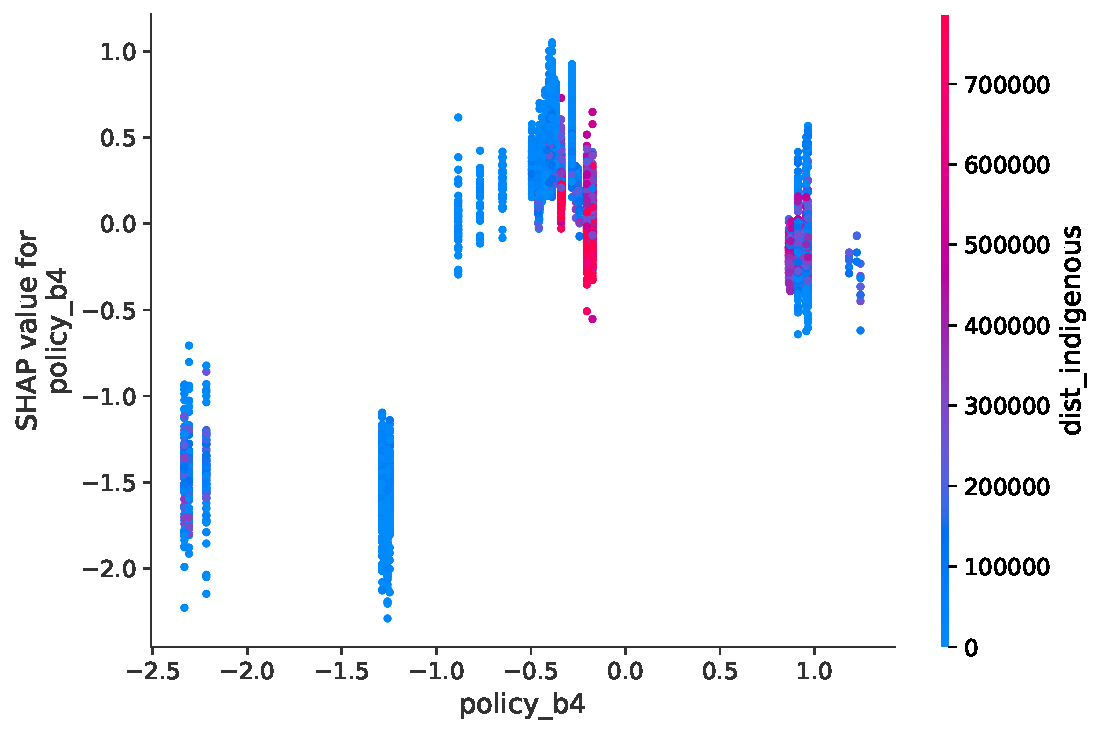
\includegraphics[width=\textwidth, keepaspectratio]{../outputs/south_america/results/model1_lgbm/shap_dep_policy_b4.pdf}
  \caption{SHAP dependence plot for \texttt{policy\_b4} (WGI Rule of Law, country level).
  The monotone positive relationship shows that stronger rule-of-law institutions are
  associated with a higher marginal SHAP contribution towards designation, consistent
  with governance quality carrying predictive information beyond ecological covariates.}
  \label{fig:shap_dep_pol}
\end{subfigure}

\vspace{1em}

\begin{subfigure}[t]{0.48\textwidth}
  \centering
  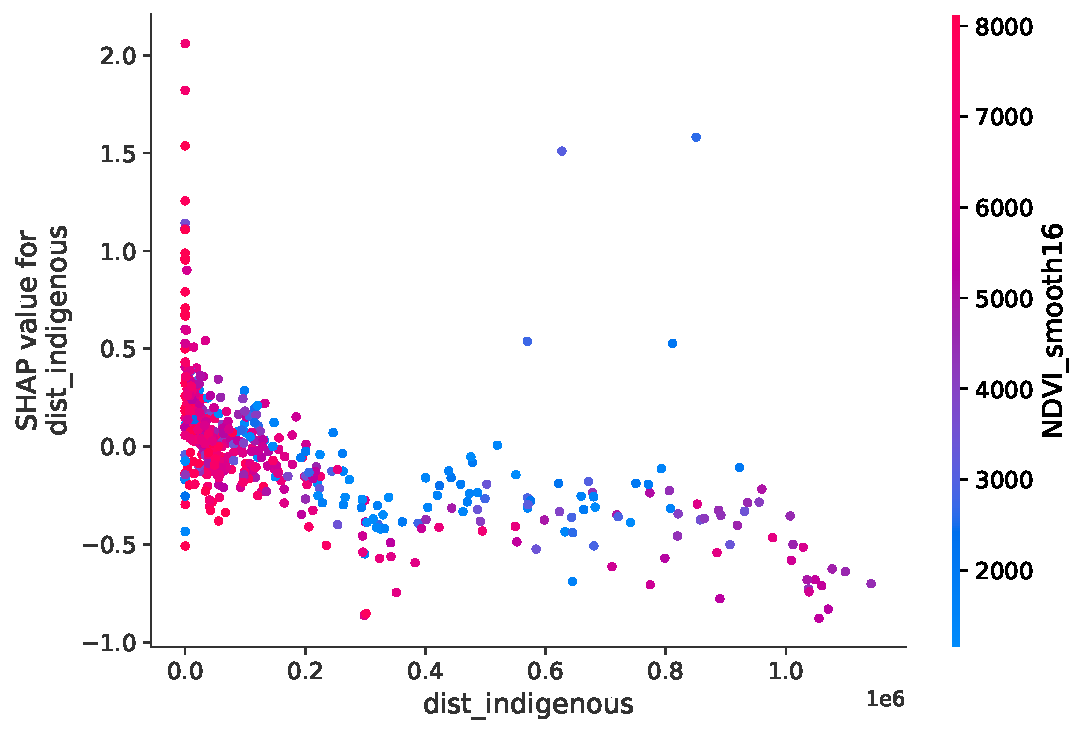
\includegraphics[width=\textwidth, keepaspectratio]{../outputs/south_america/results/model1_lgbm/shap_dep_dist_indigenous.pdf}
  \caption{SHAP dependence plot for \texttt{dist\_indigenous} (distance to nearest
  indigenous or community-managed land, km). Proximity to indigenous territories is
  associated with higher designation probability, consistent with co-management pathways
  and the overlap between indigenous territories and high-biodiversity areas in the Amazon.}
  \label{fig:shap_dep_indigenous}
\end{subfigure}
\hfill
\begin{subfigure}[t]{0.48\textwidth}
  \centering
  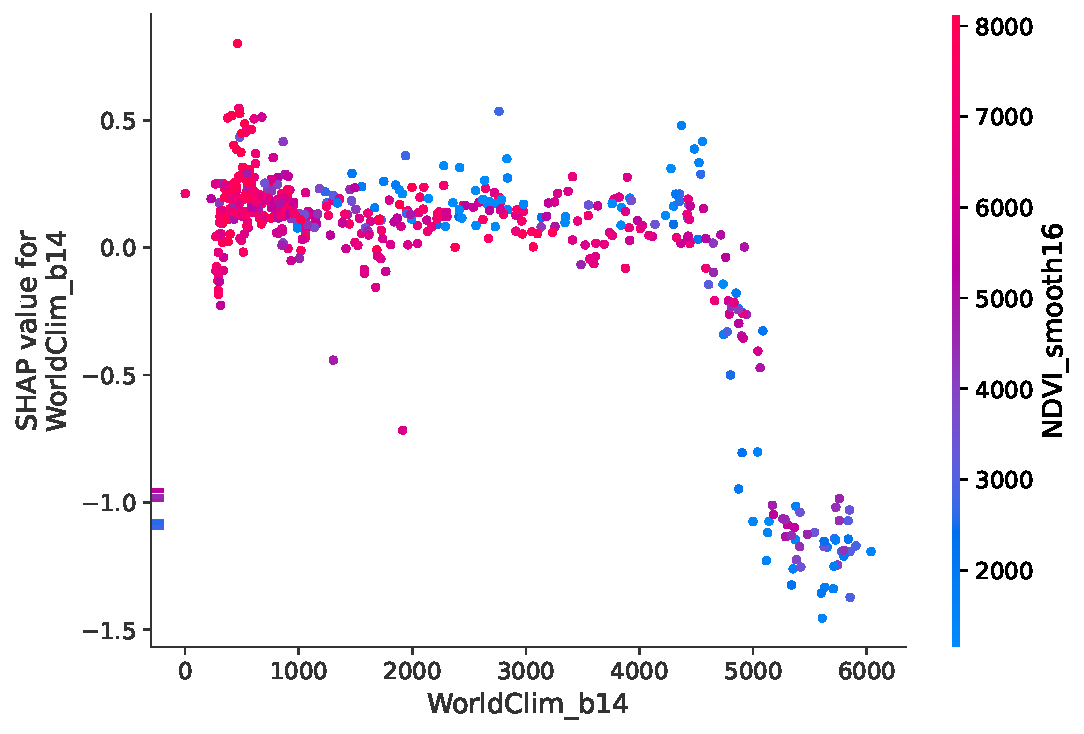
\includegraphics[width=\textwidth, keepaspectratio]{../outputs/south_america/results/model1_lgbm/shap_dep_WorldClim_b14.pdf}
  \caption{SHAP dependence plot for \texttt{WorldClim\_b14} (precipitation of the driest
  month, mm). The positive SHAP at low and high extremes reflects the model's use of
  climate envelope information: both hyper-arid and wet-season-dominated regimes exhibit
  distinctive spatial designation patterns.}
  \label{fig:shap_dep_clim}
\end{subfigure}
\caption{SHAP dependence plots for the four most important features of the South America LightGBM model.}
\label{fig:shap_dep_all}
\end{figure}

\section{Colombia Sub-Region Results}
\label{app:colombia}

A fully separate pipeline was implemented for Colombia as a computational testbed
during early model development. On the Colombia test set (2017--2019), the LightGBM
model achieves ROC-AUC 0.946 and PR-AUC 0.470; the Random Forest achieves ROC-AUC
0.931 and PR-AUC 0.435. These results provide a scale validation: the framework
performs consistently at the national level, confirming that the continental model's
discrimination is not simply a product of aggregating heterogeneous sub-regions or
its larger sample size.

\end{appendices}

\end{document}
